%% HEADER
%%%%%%%%%%%%%%%%%%%%%%%%%%%%%%%%%%%%%%%%%%%%%%%%%%%%%%%%%%%%%
\documentclass[a4paper,twoside,12pt,appendixprefix=true,bibliography=totoc,listof=totoc]{scrbook}


%% Sprache Anpassungen %%%%%%%%%%%%%%%%%%%%%%%%%%%%%%%%%%%%%
\usepackage[german,british]{babel}
\usepackage[T1]{fontenc}
\usepackage[utf8]{inputenc}

\usepackage{lmodern} %Type1-Schriftart für nicht-englische Texte


%% Packages für Grafiken & Abbildungen %%%%%%%%%%%%%%%%%%%%%%
\usepackage{caption}
\usepackage{subcaption}%%Teilabbildungen in einer Abbildung
\usepackage{graphicx} %%Zum Laden von Grafiken
\usepackage[table,xcdraw]{xcolor}

%% Packages für Formeln %%%%%%%%%%%%%%%%%%%%%%%%%%%%%%%%%%%%%
\usepackage{amsmath,amsthm,amssymb,amsfonts,mathtools}
\usepackage{bbm} %für fette Ziffern, Nummern ect. 
\usepackage{bm} %fette griechische Buchstaben


%% Zeilenabstand %%%%%%%%%%%%%%%%%%%%%%%%%%%%%%%%%%%%%%%%%%%%
\usepackage{setspace}
%\singlespacing        %% 1-zeilig (Standard)
   %% 1,5-zeilig
%\doublespacing        %% 2-zeilig

%% Verzeichnisse

%Appendix
\usepackage[toc, title, titletoc]{appendix}

%Biblatex
\usepackage[backend=biber, citestyle=authoryear,bibstyle=authoryear,giveninits=true,uniquename=init]{biblatex}
\renewbibmacro{in:}{%
  \ifboolexpr{%
     test {\ifentrytype{article}}%
     or
     test {\ifentrytype{incollection}}%
  }{}{\printtext{\bibstring{in}\intitlepunct}}%
}
\DefineBibliographyExtras{british}{\def\finalandcomma{\addcomma}} %Oxford comma
\usepackage{csquotes}
\addbibresource{Literatur.bib}

\usepackage{hyperref} %For clickable references


%% Andere Packages %%%%%%%%%%%%%%%%%%%%%%%%%%%%%%%%%%%%%%%%%%


%%Pdf Version for pdflatex
\pdfminorversion=7

%%Custom Commands
\DeclarePairedDelimiter\abs{\lvert}{\rvert}%ABS
\DeclarePairedDelimiter\norm{\lVert}{\rVert}%Norm
\newcommand{\ClOp}{\mathcal{C}} %geschwungenes C für CoDA Funktion
\newcommand{\SigA}{\mathcal{F}} %geschwungenes F für die Sigma Algebren
\newcommand{\loglik}{\ell} %geschwungenes l für die log likelihood function
\newcommand{\Tsp}{\mathcal{T}} %geschwungenes T für den T-Space
\DeclareMathOperator*{\argmax}{arg\,max} %Argmax operator
\DeclareMathOperator*{\argmin}{arg\,min} %Argmin operator




%%
\makeindex

\graphicspath {{Graphiken/}}

%%%%%%%%%%%%%%%%%%%%%%%%%%%%%%%%%%%%%%%%%%%%%%%%%%%%%%%%%%%%%
%% DOKUMENT
%%%%%%%%%%%%%%%%%%%%%%%%%%%%%%%%%%%%%%%%%%%%%%%%%%%%%%%%%%%%%
\begin{document}

\pagenumbering{Alph}
\pagestyle{empty} %%Keine Kopf-/Fusszeilen auf den ersten Seiten.
\begin{titlepage}
  %\vspace*{-1.5cm}
  \begin{center}
    
\includegraphics[width=0.45\textwidth]{TULogo.eps}
    \vskip 1cm
    {\LARGE D~\Large I~P~L~O~M~A~R~B~E~I~T}
    \vskip 8mm
    {\huge\bfseries Statistical models for multivariate (compositional) count time series}
    \vskip 8mm
    \large 
    Zur Erlangung des akademischen Grades
    \vskip 5mm
    {\Large\bfseries Diplom-Ingenieur}
    \vskip 5mm
    Im Rahmen des Masterstudiums
    \vskip 5mm
    {\Large\bfseries Wirtschaftsmathematik und Statistik}
    \vskip 5mm
    {Ausgef\"uhrt am}
    \vskip 5mm
    {\Large Institut f\"ur Stochastik und Wirtschaftsmathematik}\\[1ex]
    {\Large Fakult\"at f\"ur Mathematik und Geoinformation}\\[1ex]
    {\Large Technische Universit\"at Wien}
    \vskip 5mm
    Unter der Anleitung von
    \vskip 5mm
    {\Large\bfseries Univ.Prof. Dipl.-Ing. Dr.techn. Peter Filzmoser}
    \vskip 5mm
    Eingereicht von
    \vskip 5mm
    {\Large\bfseries Alexander Schwaiger, BSc}\\[1ex]
    Matrikelnummer: {11775205}
  \end{center}
  
  \vfill
  
  \small
\begin{tabular}{cccc}
Wien, am {\today} & & \makebox[4.21cm]{\hrulefill} & \makebox[4.21cm]{\hrulefill}\\
 & & Alexander Schwaiger (Verfasser) & Peter Filzmoser (Betreuer)
\end{tabular}
\end{titlepage}

\cleardoublepage

\pagestyle{plain} %%Ab hier die Kopf-/Fusszeilen

\onehalfspacing    % Ab hier 1.5 Zeilenabstand

\pagenumbering{roman}
\addchap{Abstract}
In this thesis, we analyse and compare two approaches for multivariate count data time series with an excessive amount of zeros. The first approach belongs to the class of generalised linear models (GLM) and fits a univariate integer valued generalized autoregressive conditional heteroskedasticity model of order (p,q) (INGARCH(p,q) model) for each dimension. The second approach is based on compositional data analysis (CoDA) and uses the relative structure of our data to build a vectorised autoregressive (VAR) model from it. In addition, we also consider alternative options like zero-inflated models and integer-valued autoregressive (INAR) models. Providing the mathematical background for the INGARCH(p,q) and CoDA approach and exploring different parameter settings of them, we evaluate their performance on real world data and compare different tuning options. We then introduce an error measure for comparison and use it to compare the performance on different time series. At last, we provide a handbook of our analysis in the statistical software R and present the used packages and functions. \newline

\textbf{Keywords:} Compositional Data Analysis, General Linear Models, INGARCH, Multivariate Count Data Time Series, R
\chapter*{Kurzfassung}
\begin{otherlanguage}{german}

In dieser Diplomarbeit werden zwei Ansätze für multivariate Zähldaten-Zeitreihen mit einer überproportionalen Anzahl von Nullern analysiert und verglichen. Der erste Ansatz gehört zu der Klasse der verallgemeinerten linearen Modelle (GLM). Dabei wird ein ganzzahliges verallgemeinertes autoregressives Model mit bedingter Heteroskedastizität der Ordnung (p,q) (INGARCH(p,q) Model) für jede Dimension gefitted. Der zweite Ansatz basiert auf der Analyse von Kompositionsdaten (CoDA) und nutzt die relative Struktur der Daten, um daraus ein vektorisiertes autoregressives Model (VAR) zu erstellen. Darüber hinaus betrachten wir auch alternative Optionen wie Zero-Inflation-Modelle (ZIM) und ganzzahlige autoregressive Modelle (INAR). Wir beschreiben den mathematischen Hintergrund des INGARCH(p,q)- und des CoDA-Ansatzes, untersuchen verschiedene Parametereinstellungen, vergleichen Tuning-Optionen und testen die Modelle mit realen Daten. Anschließend führen wir ein Fehlermaß zum Vergleich ein und verwenden es, um die Güte der Modelle bei verschiedenen Zeitreihen zu vergleichen. Schließlich stellen wir ein Benutzerhandbuch für unsere Analyse in der Statistiksoftware R zur Verfügung und präsentieren die verwendeten Pakete und Funktionen. \newline

\textbf{Schlagworte:} Compositional Data Analysis, General Linear Models, INGARCH, Multivariate Count Data Time Series, R

\end{otherlanguage}
\chapter*{Eidesstattliche Erklärung}
\thispagestyle{empty}
\vspace*{2cm}

Ich erkläre an Eides statt, dass ich die vorliegende Diplomarbeit selbstständig und ohne fremde Hilfe verfasst, andere als die angegebenen Quellen und Hilfsmittel nicht benutzt bzw. die wörtlich oder sinngemäß entnommenen Stellen als solche kenntlich gemacht habe.

\vspace*{3cm}

\noindent
Wien, am {\today} %\today
%
\hfill 
%
\begin{minipage}[t]{5cm}
	\centering
		\raisebox{-4ex}{
\includegraphics[width=1.00\textwidth]{Unterschrift003.jpg}}
\underline{\hspace*{5cm}}\\
\small {Alexander Schwaiger}
\end{minipage}
\chapter*{Acknowledgements}
At this point, I would like to express my sincere gratitude to my supervisor Univ.Prof. Dipl.-Ing. Dr.techn. Peter Filzmoser for the help he provided in the form of resources, answers to my questions and in general the excellent guidance during my thesis. In this context I also have to thank Dipl.-Ing. Lukas Neubauer who worked on this project with me and supported me not only in the analysis and interpretation of the results but also with suggestions and insightful comments. I also want to thank Schrankerl GmbH for providing the data used for carrying out the analyis.

Furthermore, I would like to thank my family and especially my parents who gave me the opportunity to study and supported me the whole time. I also want to thank my friends and colleagues who accompanied me during this journey and made this an unforgettable time. 
%% Inhaltsverzeichnis %%%%%%%%%%%%%%%%%%%%%%%%%%%%%%%%%%%%%%%
\tableofcontents %Inhaltsverzeichnis
\cleardoublepage %Das erste Kapitel soll auf einer ungeraden Seite beginnen.
\pagenumbering{arabic} 

%%%%%%%%%%%%%%%%%%%%%%%%%%%%%%%%%%%%%%%%%%%%%%%%%%%%%%%%%%%%%
%% HAUPTTEIL MIT KAPITEL
%%%%%%%%%%%%%%%%%%%%%%%%%%%%%%%%%%%%%%%%%%%%%%%%%%%%%%%%%%%%%
\chapter{Introduction}
\label{sec:Introduction}
\section{Motivation}
\label{sec:Motivation}

Multivariate count data is a reoccurring theme in real-world applications. While there are various methods among the classical statistical models to handle such data, there are fewer methods available to handle it in a time series context. Even more so, when there is an excessive amount of zeros or missing values present. In this thesis, we compare various models for such data and compare their predictive power. We test our models on real world data, which was kindly provided to us, and analyse their performance. In the following, we will shortly describe the general framework and objective. 

This thesis is part of a bigger project carried out at the Technical University of Vienna in cooperation with the company Schrankerl GmbH. Schrankerl GmbH operates food vending machines in offices, which are filled with food ranging from appetizers and main course to snacks and beverages. Each week the vending machines, or in the following also called fridges, are being restocked and the number of items sold in the past week is being recorded. In addition, non-sold items are being disposed of which results in monetary losses. The objective is to find a model to predict the amount the company needs to order for the upcoming week, in a bid to minimise the loss.

\section{Data Description}
\label{sec: Data Description}

In this section, we describe the structure of our data, which is essential in choosing the right model. We have several multivariate time series with integer values, with each series representing a vending machine. The dimensions represent the various categories of the food where each item is of one of the four main categories 1,2,3,4 and one of the various subcategories. We mainly analyse the time series on the aggregated level of the main categories; however, the models can also be applied to the subcategories. In this case we have a model for each main category instead of each vending machine. The values for each category represent the number of items sold. For a fridge $f$ denote this time series with 
%
\begin{equation}
\left\{\bm{Y}_t:t=1,\ldots,T_f; \bm{Y}_t \in \mathbb{N}_0^K \right\}_f,
\label{eq:time series definition}
\end{equation}
%
where $K$ stands for the number of categories, $T_f$ denotes the total length of the time series and $\mathbb{N}_0^K = \underbrace{\mathbb{N}_0 \times \ldots \times \mathbb{N}_0}_{K-times}$. This means $\bm{Y}_t = (Y_{1t},\ldots,Y_{Kt})^T$ with $Y_{kt} \in \mathbb{N}_0, t=1,\ldots,T_f$ and $k=1,\ldots,K$. Since we will sometimes not use all of our data but only a fraction of it, we will denote with $T$ the length of the time series used

\begin{equation}
\left\{\bm{Y}_t:t=1,\ldots,T; \bm{Y}_t \in \mathbb{N}_0^K \right\}_f.
\label{eq:time series definition fraction}
\end{equation}
%
So Equation (\ref{eq:time series definition}) describes the whole time series available, while Equation (\ref{eq:time series definition fraction}) describes the time series used and it holds $T\leq T_f$. In the following we will use Equation (\ref{eq:time series definition fraction}) to indicated that we may only use a fraction of the whole time series. We will dive more into that in Section \ref{sec: Model Specification}.

The data is measured on a weekly basis and hence our points in time are equidistant. One noteworthy feature of our data is the amount of 0 and NA values, which will be dived into in later sections. An additional characteristic of our data is the difference in length for various time series. While for some time series we have 70+ data points, for others we have less than 10. An example view of our data would be: 

\begin{table}[h!]
\centering
\begin{tabular}{ccccc}
\hline
\rowcolor[HTML]{FFFFFF} 
\textbf{Fridge ID} & \textbf{Week Date} & \textbf{Main Category} & \textbf{Sub Category} & \textbf{Sold} \\ \hline
111                & 2021-01-18         & 1                      & 3                     & 6             \\
111                & 2021-01-18         & 1                      & 8                     & 7             \\
111                & 2021-01-25         & 2                      & 6                     & 4             \\
222                & 2022-06-06         & 3                      & 15                    & 1             \\
222                & 2022-06-06         & 4                      & 11                    & 0             \\
222                & 2022-06-13         & 1                      & 100061                & 0             \\
222                & 2022-06-20         & 2                      & 6                     & 30            \\
222                & 2022-06-20         & 2                      & 10                    & 15            \\ \hline
\end{tabular}
\caption{Example data}
\label{tab:ExampleData}
\end{table}
%
As mentioned before, we mainly aggregate our data on main category level. This means that we do not differentiate between the subcategories and are only interested in the number of items sold for each main category. Our data in Table \ref{tab:ExampleData} would then change to Table \ref{tab:ExampleData aggregated}:

\begin{table}[h!]
\centering
\begin{tabular}{cccc}
\hline
\rowcolor[HTML]{FFFFFF} 
\textbf{Fridge ID} & \textbf{Week Date} & \textbf{Main Category} & \textbf{Sold} \\ \hline
111                & 2021-01-18         & 1                      & 13             \\
111                & 2021-01-25         & 2                      & 4             \\
222                & 2022-06-06         & 3                      & 1             \\
222                & 2022-06-06         & 4                      & 0             \\
222                & 2022-06-13         & 1                      & 0             \\
222                & 2022-06-20         & 2                      & 45            \\ \hline
\end{tabular}
\caption{Example data aggregated on main category level}
\label{tab:ExampleData aggregated}
\end{table}

\section{Outlook}
\label{sec: Outlook}

The remainder of the thesis is split in the following way. In Chapters \ref{sec:CountTS} and \ref{sec:Coda}, we describe our methodologies used and the reasoning why we are using them. We provide a short literature review about count data time series in Section \ref{sec:CountTS}. In these chapters, we also lay the mathematical groundwork for the considered methods. In Chapter \ref{sec:Application}, we explain the specification and tuning options for our models and also introduce an error measure to evaluate their performance. We show the results on some exemplary time series and then show the results of each tuning parameter. In Section \ref{sec:R-Code}, we explain the R-functions used and provide a guidebook.% In the conclusion \ref{sec: Conclusion} we summarise our findings and provide a further outlook on the topic. 

\chapter{Count Time Series Models}
\label{sec:CountTS}
\section{INGARCH}
\label{sec:Ingarch}

In this section we introduce the INGARCH(p,q), in short just INGARCH, model. First we provide a motivation on why we chose this model and review some other possible models for discrete time series count data. The review is mainly based on \cite{Liboschik:2016} and \cite{Heinen:2003}. A more detailed review can be found in \cite{Zucchini:1997}. Subsequently we define the INGARCH(p,q) model itself and list some of its properties. 

\subsection{Motivation}
\label{sec:Ingarch Motivation}

This section is based on \cite{Liboschik:2016} and \cite{Heinen:2003}. \newline
Since our data can be seen as a discrete time series with count data, we want a model which is able to take these properties into account. In addition, autocorrelation and over dispersion are two common features in count data. 
 
One common way to deal with count data are Markov chains. The dependent variable can take on all possible values in the so called state space and the probability of changing states is then modelled as a transition probability. A limitation is the fact that these models become cumbersome if the state space gets too big and lose tractability. As an extension to the basic Markov chains models, Hidden Markov chains are proposed by \cite{Zucchini:1997}. However, since there is no generally accepted way to determine the order of this model, it can cause problems if the data structure does not provide intuitive ways to do it. Another issue is that the number of parameters which need to be estimated gets big quickly, especially if the order of the model is big. 

Other common models for time series data are the ARMA models. There exists a discrete version of them in the form of the Discrete Autoregressive Moving Average (DARMA) models. They can be defined as a mixture of discrete probability distributions and a suitable chosen marginal probability function \cite{Biswas:2009}. While there have been various applications, for example in \cite{Chang:1987}, there seem to be difficulties in their estimation \cite{Heinen:2003}. 

State space models with conjugated priors are proposed by \cite{Harvey:1989}. The observations are assumed to be drawn from a Poisson distribution whose mean itself follows a Gamma distribution. The parameters of the Gamma distribution are chosen in such a way that its mean is constant but its variance is increasing. While there are ways proposed by \cite{Qaqish:1988} to handle overdispersion, these models have the weakness of needing further assumptions to handle zeros while also having more complicated model specifications \cite{Heinen:2003}.

While there are many more possible models, we decided to focus on the class of Generalised Linear Models (GLM). In the case of discrete time series with count data, the observations are modelled conditionally on the past and follow a discrete distribution. The conditional mean is then connected with a link function to the past observations and conditional means. Furthermore, a covariate vector can be introduced to account for external influence. While being easy to use and estimate they still provide a good amount of flexibility. In addition, a wide array of tools is available for various tests and forecasts. From the class of the GLMs we compare the INGARCH(p,q) and a log-linear model, which will be discussed in section \ref{sec: Other methods}. We then chose the INGARCH(p,q) model based on its superior performance and stability.

We also introduce an extension of the INGARCH model to multivariate data. However, since to our knowledge there is currently no R-package available to fit these models, we stay with the univariate version. 


\subsection{INGARCH Model}
\label{sec:Ingarch Model}
We construct the INGARCH(p,q) model as in \cite{Liboschik:2016}. 
Take again our time series $\left\{\bm{Y}_t:t=1,\ldots,T; \bm{Y}_t \in \mathbb{N}_0^K \right\}_f$ for fridge $f$ and denote the univariate time series for category $k$ with $\left\{Y_{kt}:t=1,\ldots,T; Y_{kt} \in \mathbb{N}_0\right\}_f$  for $k=1,\ldots,K$. This means $\bm{Y}_t = (Y_{1t},\ldots,Y_{Kt})^T$. Denote a r-dimensional time varying covariate vector with $\textbf{X}_{kt}=(X_{t1}^k,\ldots,X_{tr}^k)^T$. Let the conditional mean be $\lambda_{kt} = \mathbb{E}\left[Y_{kt} | \SigA_{k,t-1} \right]$ where $\SigA_{k,t-1}$ is the $\sigma$-field generated by $Y_{kt}$ and $\lambda_l$ for $l<t$ $, \SigA _{k,t-1}= \sigma(Y_{k1},\ldots,Y_{kl},\lambda_1, \ldots, \lambda_l)$. Therefore, the conditional mean of the time series is dependent on its combined history of the past conditional means and its past values. With this, we can define the integer valued generalized autoregressive conditional heteroskedasticity model of order (p,q) (INGARCH(p,q) model) for category $k=1,\ldots,K$ as,

\begin{gather}
\label{eq:Ingarch model}
Y_{kt} | \SigA_{k,t-1} \sim P(\lambda_{kt}); \forall t \in \mathbb{N}, \\
\mathbb{E}\left[Y_{kt} | \SigA_{k,t-1} \right] = \lambda_{kt} = \beta_0 + \sum_{i=1}^p\beta_i Y_{k,t-i} + \sum_{j=1}^q\alpha_j \lambda_{k,t-j},
\end{gather}

where $p,q \in \mathbb{N}$ and $P(\lambda_{kt})$ is a Poisson distribution with mean $\lambda_{kt}$. The integer $p$ defines the number of past values to regress on, whereas $q$ does the same for the past conditional means. In order to account for external effects as well, we add the covariate vector $\textbf{X}_{kt}$

\begin{gather}
\label{eq:Ingarch model with external effect}
Y_{kt} | \SigA_{k,t-1} \sim P(\lambda_{kt}); \forall t \in \mathbb{N}, \\
\mathbb{E}\left[Y_{kt} | \SigA_{k,t-1} \right] = \lambda_{kt} = \beta_0 + \sum_{i=1}^p\beta_i Y_{k,t-i} + \sum_{j=1}^q\alpha_j \lambda_{k,t-j} + \bm{\eta}^T\textbf{X}_{kt},
\end{gather}

where $\bm{\eta}$ is the parameter for the covariates such that $\bm{\eta}^T\textbf{X}_{kt} \geq 0$.
From the distributional assumption $Y_{kt} | \SigA_{k,t-1} \sim P(\lambda_{kt})$ it follows

\begin{equation}
p_{kt}(y;\bm{\theta})=\mathbb{P}(Y_{kt}=y | \SigA_{k,t-1}) = \frac{\lambda_{kt}^y \exp(-\lambda_{kt})}{y!}, \hspace{0.2cm} y \in \mathbb{N}_0.
\label{eq:Ingarch Distribution}
\end{equation}

Furthermore it can be shown that conditionally on the past history $\SigA_{k,t-1}$ the model is equidispersed, i.e. it holds $\lambda_{kt} = \mathbb{E}\left[Y_{kt} | \SigA_{k,t-1}\right] = \mathbb{V}\left[Y_{kt} | \SigA_{k,t-1}\right]$. However, unconditionally the model exhibits overdispersion. In that case it holds $\mathbb{E}\left[Y_{kt}\right] \leq \mathbb{V}\left[Y_{kt}\right] $ \cite{Heinen:2003}. 

\subsubsection{Parameter Estimation and Forecasting}
\label{sec: Estimation of the Ingarch Model}

We summarise the estimation of the INGARCH(p,q) Model as described in \cite{Liboschik:2016}. The model is estimated for each category $k=1,\ldots,K$ separately. 

The parameter space for the INGARCH(p,q) model with external effects \ref{eq:Ingarch model with external effect} is given by 

\begin{equation}
\Theta = \left\{ \bm{\theta} \in \mathbb{R}^{p+q+r+1}: \beta_0 > 0, \beta_1,\ldots,\beta_p,\alpha_1,\ldots,\alpha_q,\eta_1,\ldots,\eta_r \geq 0, \sum_{i=1}^p\beta_i + \sum_{j=1}^q\alpha_j < 1 \right\}.
\label{eq:Ingarch parameter space}
\end{equation}

To ensure positivity of the conditional mean $\lambda_{kt}$, the intercept $\beta_0$ must be positive while all other parameters must be non negative. The upper bound of the sum ensures that the model has a stationary and ergodic solution with moments of any order \cite{Ferland:2006,Fokianos:2009,Doukhan:2012}. A quasi maximum likelihood approach is used to estimate the parameters $\bm{\theta}$. 
For observations $\textbf{y}_k = \left(y_{k1},\ldots,y_{kT}\right)^T$ for category $k=1,\ldots,K$, the conditional quasi log-likelihood function, up to a constant, is given by,

\begin{equation}
\loglik_k(\bm{\theta}) = \sum_{t=1}^T\log p_{kt}(y_{kt};\bm{\theta}) = \sum_{t=1}^T \left(y_{kt}\log(\lambda_{kt}(\bm{\theta})) - \lambda_{kt}(\bm{\theta})\right).
\label{eq: Quasi log likelihood}
\end{equation}

where $p_{kt}(y_{kt};\bm{\theta})$ is the probability density function defined in \ref{eq:Ingarch Distribution}. The conditional mean is seen as a function $\lambda_{kt}: \Theta \rightarrow \mathbb{R}^{+}$. The conditional score function is given by,

\begin{equation}
S_{kT}(\bm{\theta}) = \frac{\partial \loglik_k(\bm{\theta})}{\partial \bm{\theta}} = \sum_{t=1}^T\left(\frac{y_{kt}}{\lambda_{kt}(\bm{\theta})}-1\right)\frac{\partial\lambda_{kt}(\bm{\theta})}{\partial \bm{\theta}}.
\label{eq:conditional score}
\end{equation}

The vector $\frac{\partial\lambda_{kt}(\bm{\theta})}{\partial \bm{\theta}}$ can be computed recursively. 
The conditional information matrix is given by, 

\begin{align}
G_{kT}(\theta) &= \sum_{t=1}^T Cov\left(\frac{\partial \loglik_k(\bm{\theta}; Y_{kt})}{\partial \bm{\theta}} \middle| \SigA_{k,t-1}\right) \\
&=  \sum_{t=1}^T \left(\frac{1}{\lambda_{kt}\left(\bm{\theta}\right)}\right) \left(\frac{\partial \lambda_{kt}(\bm{\theta})}{\partial \bm{\theta}}\right)\left(\frac{\partial \lambda_{kt}(\bm{\theta})}{\partial \bm{\theta}}\right)^T.
\label{eq:conditional information matrix}
\end{align}

Finally, assuming that the quasi maximum likelihood estimator (QMLE) $\hat{\bm{\theta}}_T$ of $\bm{\theta}$ exists, it is the solution to 

\begin{equation}
\hat{\bm{\theta}}:= \hat{\bm{\theta}}_T = \text{arg max}_{\bm{\theta} \in \Theta} (\loglik_k(\bm{\theta})). 
\label{eq:ingarch qmle}
\end{equation}

The optimal one-step ahead forecast with regards to the mean squared error is the conditional expectation $\lambda_{k,t+1}=\mathbb{E}\left[Y_{k,t+1} | \SigA_{kt} \right]$. The h-step ahead prediction for $h>1$ is calculated iteratively with the one step ahead predictions of $Y_{k,t+1},Y_{k,t+2},\ldots$ \cite{Liboschik:2016}. 


\subsection{Multivariate INGARCH model}
\label{sec: Multivariate Ingarch}

Since we have multivariate data, we also investigate multivariate versions of the INGARCH model. There have been various approaches in literature to expend the univariate INGARCH model to more dimensions. Bivariate models have been proposed by \cite{Liu:2012} and  extended for example by \cite{Cui:2018}. The authors in \cite{Fokianos:2020,Fokianos:2021} introduce and review the multivariate INGARCH model on the basis of a data generating process. Let $\bm{\lambda}_t=\mathbbm{E}[\bm{Y}_t|\SigA_t]$ where $\bm{\lambda}_t = (\lambda_{1t},\ldots,\lambda_{Kt})^T$ and $\SigA_t$ is the $\sigma$-field generated by $\left\{\bm{Y}_0,\ldots,\bm{Y}_t,\bm{\lambda}_0\right\}$. Then for each $k=1,\ldots,K$ we assume

\begin{gather}
Y_{kt} | \SigA_{t-1} \sim P(\lambda_{kt}), \\
\bm{\lambda}_t = \bm{d} + \bm{A}\bm{\lambda}_{t-1} + \bm{B}\bm{Y}_{t-1}.
\label{eq:Mingarch 1}
\end{gather}

Based on this, a joint distribution is constructed using a copula structure. After an additional transformation, the multivariate INGARCH model is

\begin{gather}
\bm{Y}_t = \bm{N}_t(\bm{\lambda}_t), \\
\bm{\lambda}_t = \bm{d} + \bm{A}\bm{\lambda}_{t-1} + \bm{B}\bm{Y}_{t-1},
\label{eq:Mingarch 1 new}
\end{gather}

where $\left\{\bm{N}_t\right\}$ is a sequence of p-variate independent copula-Poisson processes that counts the number of events in $[0,\lambda_{1t}]\times,\ldots,\times[0,\lambda_{Kt}]$ \cite{Fokianos:2020}. 

Another approach is taken by \cite{Lee:2023}. Instead of constructing a joint distribution for the multivariate vector $\bm{Y}_t$, they fit a one-parameter exponential family conditional distribution to each component $Y_{kt}$

\begin{equation}
p_{k}(y|\nu) = \exp(\nu y - A_k(\nu))h_k(y), \hspace{0.5cm} y \in \mathbbm{N}_0,
\label{eq:Exponential Family}
\end{equation}

where $A_k$ and $h_k$ are known functions and $\nu$ is the natural parameter. Both $A_k$ and $B_k(\nu) = \frac{d A_k(\nu)}{d \nu}$ are strictly increasing \cite{Lee:2023}. The multivariate INGARCH model is then given for each $k=1,\ldots,K$ by

\begin{gather}
Y_{kt} | \SigA_{t-1} \sim p_k(y|\nu_{kt}), \\
\bm{\lambda}_t := \mathbbm{E}[\bm{Y}_t | \SigA_{t-1}] = f_{\theta}(\bm{\lambda}_{t-1},\bm{Y}_{t-1}),
\label{eq:Mingarch 2}
\end{gather}

where $\SigA_{t-1}$ is the $\sigma$-field generated by $\left\{\bm{Y}_{t-1},\bm{Y}_{t-2},\ldots,B_k(\nu_{kt})\right\}$ with $B_k(\nu_{kt})=\lambda_{kt}$, and $f_{\theta}$ is a non-negative function on $[0,\infty)^K \times \mathbb{N}_0^K$ \cite{Lee:2023}. So for each component $Y_{kt}$ a univariate INGARCH model is fit but the components are connected by the conditional mean process. 

%\section{Other Methods}
%\label{sec: Other methods}

\section{GARCH Models}
\label{sec: Garch Models}

INGARCH models are structurally derived from the generalised autoregressive conditional heteroscedasticity (GARCH) models, which themselves are generalisations of the autoregressive conditional heteroscedasticity (ARCH) model. ARCH models, which were first developed by Engle \textcite{Engle:1982} in an economic context, model the variance conditional on past values. Since we no longer assume our data to be integer valued, our time series has the form $\left\{Y_{kt}:t=1,\ldots T; Y_{kt} \in \mathbb{R}\right\}_f$. Denote again with $\SigA_{k,t}$ the information available at time $t$. Then the ARCH(1) model is given by \textcite{Engle:1982}

\begin{equation}
\begin{gathered}
Y_{kt} | \SigA_{k,t-1} \sim N(0,h_{kt}),\\
h_{kt} = a_0 + a_1 Y_{k,t-1}^2,
\label{eq:ARCH model}
\end{gathered}
\end{equation}
%
with $a_0\geq0$, $a_1>0$. 

The variance function can be generally formulated as $h_{kt} = h(Y_{k,t-1},\ldots,Y_{k,t-p},\bm{a})$, where $\bm{a}=(a_1,\ldots,a_p)^T\geq 0$ is the parameter vector with $a_p>0$, and $p \in \mathbbm{N}$ is the order of the ARCH process. 
The GARCH model generalises this approach by adding the past variances as another source of information. The GARCH(p,q) model for non-negative parameters $a_0>0$, $\bm{a}=(a_1,\ldots,a_q)^T\geq 0$ and $\bm{b}=(b_1,\ldots,b_p)^T\geq0$ with $p,q \in \mathbbm{N}$, $p\geq0, q>0$ is given by \textcite{Bollerslev:1986}

\begin{equation}
\begin{gathered}
Y_{kt} | \SigA_{k,t-1} \sim N(0,h_{kt}); \forall t \in \mathbbm{N}, \\
\mathbbm{V}[Y_{kt}|\SigA_{k,t-1}]=h_{kt} = a_0 + \sum_{i=1}^q a_i Y_{k,t-i}^2 + \sum_{j=1}^p b_j h_{k,t-j};\forall t \in \mathbbm{N}.
\label{eq:GARCH model}
\end{gathered}
\end{equation}
%
Other distributions than the normal distributions can be taken as well. 

\subsection{Parameter Estimation and Forecasting}
\label{sec: GARCH Parameter Estimation and Forecasting}

Estimation of the parameters can be done with maximum likelihood and an iterative algorithm. First, the model is rewritten and the logarithm of the likelihood function is taken. Second, after differentiation with respect to its variance and mean parameters, the Berndt, Hall Hall and Hausman algorithm \textcite{Berndt:1974}is used to obtain the maximum likelihood estimates. Further details and assumptions can be found in \textcite{Bollerslev:1986}. 

If one is interested in forecasting $Y_{kt}$, then the minimum mean squared one-step error forecast is $\mathbbm{E}[Y_{k,t+h}|\SigA_{k,t}]=0$ where $\SigA_{k,t}$ is the information available at time $t$. One should note, that the forecast is independent of the model parameters. If the conditional variance should be forecasted, the parameters are estimated and the known values are plugged in. For $h>1$, $h$-step predictions are computed recursively with plugging in the forecasts for $h-1,h-2,\ldots$ in the model \textcite{Zivot:2009}. 


\subsection{Testing for GARCH Models}
\label{sec: Testing for GARCH models}

To decide whether to use a GARCH model, one can test for volatility or the validity of GARCH models in general. In the original paper \textcite{Bollerslev:1986}, the author suggests a Lagrange multiplier test. Other popular tests include the Box–Pierce–Lung‐type portmanteau tests and residual‐based diagnostics \textcite{Hong:2017}. The authors in \textcite{Hong:2017} present further methods. 


\subsection{Applications}
\label{sec: Garch Applications}

The introduction of ARCH and subsequently GARCH models in the 1980s has been revolutionary. ARCH models have originally been introduced for modelling macroeconomic key figures such as inflation rates but since then have been used in a variety of fields. GARCH models generalised the ARCH model approach to allow the modelling of a more flexible lag structure \textcite{Bollerslev:1986}. They have found wide applications in finance mathematical problems, especially for the modelling of a changing variance and volatility in financial markets. They are often used to estimate volatility of various financial instruments. 

Since the ARCH and GARCH models are used to model and forecast volatility or the conditional variance, but not values, we will not use it in our application. In addition, the INGARCH model also accounts for the discrete nature of our data, which makes it the preferred choice. 


\section{Naive Random Walk}
\label{sec: Naive Random Walk}

The Naive Random Walk model is one of the simplest and most comprehensive forecasting models, which makes it a popular benchmark model. In addition, it is what is currently employed, so using it enables us to directly see if our models outperform the current model. It assumes that the 1-step difference between two values is i.i.d distributed with mean 0. Let $\left\{Y_{kt}:t=1,\ldots T; Y_{kt} \in \mathbb{N}_0\right\}_f$ be our univariate time series. Then the Naive Random Walk model is given as

\begin{equation}
Y_{k,t+1}= Y_{kt} + \epsilon_{kt}, 
\label{eq: Random Walk Model}
\end{equation}
 %
where $\epsilon_{kt} \sim WN(\sigma_k^2)$ is a white noise process with variance $\sigma_k^2 \in \mathbb{R}_+$. It can be shown easily, that the optimal 1-step ahead forecast with regard to the mean squared error (MSE) is given by

\begin{equation}
\hat{Y}_{k,t+1}= Y_{kt},
\label{eq: Random Walk Model Prediction}
\end{equation}
%
where $\hat{Y}_{k,t+1}$ is the predicted value at time $t+1$. In other words, the predicted value is the last known value.  


\section{Zero-Inflated Models}
\label{sec: Zim}

Since we encounter a large number of zeros, we also consider zero-inflated models. Zero inflation means that the proportion of observed zeros is bigger than that of the underlying distribution and hence would not be expected. The idea of zero-inflated models is to add a degenerated distribution with mass at zero to the probability mass function, which enables one to explain the large amount of zero values. The probability mass function of a $ZIP(\lambda,\omega)$ distribution for a random variable $Y$ is defined as \textcite{Zhu:2012}

\begin{equation}
\mathbb{P}(Y=y) = \omega \delta_{y,0}+ (1-\omega) \frac{\lambda^y \exp(-\lambda)}{y!}, \hspace{0.2cm} y \in \mathbb{N}_0.
\label{eq:ZIP Distribution}
\end{equation}
%
where $0 < \omega < 1$ is the zero-inflation parameter, $\lambda$ is the Poisson parameter and $\delta_{y,0}$ is the Kronecker delta for which $\delta_{y,0}=1$ if $y=0$ and $\delta_{y,0}=0$ else. This way our zeros can come from two different sources \textcite{Zhu:2012}. The first part of Equation (\ref{eq:ZIP Distribution}) $\delta_{y,0}$ is the degenerated point mass distribution.

Let $\SigA_{k,t-1}$ be the $\sigma$-field generated by $\left\{Y_{k,t-1},Y_{k,t-2},\ldots\right\}$. Assume, conditionally on $\SigA_{k,t-1}$, that $Y_{k,1},\ldots,Y_{k,T}$ are independent. Now we can define the Zero-Inflated Poisson (ZIP) INGARCH(p,q) as

\begin{equation}
\begin{gathered}
\label{eq:ZIP model}
Y_{kt} | \SigA_{k,t-1} \sim ZIP(\lambda_{kt},\omega_k); \forall t \in \mathbb{N}, \\
\mathbb{E}\left[Y_{kt} | \SigA_{k,t-1} \right] = \lambda_{kt} = \beta_0 + \sum_{i=1}^p\beta_i Y_{k,t-i} + \sum_{j=1}^q\alpha_j \lambda_{k,t-j},
\end{gathered}
\end{equation}
%
with $0<\omega_k<1$, $\beta_0>0$, $\beta_i\geq 0$, $\alpha_j \geq 0$ for $i=1,\ldots,p$, $j=1,\ldots,q$, $p\geq 1$, $q\geq 0$ \textcite{Zhu:2012}. If $\omega_k =0$ then we get the standard INGARCH(p,q) model discussed above. It can be shown that the conditional mean and variance are given by

\begin{equation}
\mathbb{E}[Y_{kt} | \SigA_{k,t-1}] = (1-\omega_k)\lambda_{kt}, \hspace{1cm} \mathbb{V}[Y_{kt} | \SigA_{k,t-1}] =(1-\omega_k)\lambda_{kt}(1+\omega_k \lambda_{kt}),
\label{eq:Conditional Mean and Variance ZIP}
\end{equation}
%
which implies $ \mathbb{V}[Y_{kt} | \SigA_{k,t-1}] > \mathbb{E}[Y_{kt} | \SigA_{k,t-1}]$ \textcite{Zhu:2012}. This means that Model (\ref{eq:ZIP model}) can handle overdispersion in our data. More details about zero-inflated models and especially the zero-inflated INGARCH(p,q) model can be found in \textcite{Zhu:2012}.

However, due to a lack of available R-packages for zero-inflated Poisson INGARCH models, we use a zero-inflated Poisson autoregressive model. We assume that we have discrete count data $\left\{Y_{kt}\right\}$ which is conditionally $ZIP(\lambda_{kt},\omega_{kt})$ distributed. For the parameters $\lambda_{kt}$ and $\omega_{kt}$, the ZIP autoregressive model is given by \textcite{Yang:2012}

\begin{equation}
\begin{gathered}
Y_{kt} | \SigA_{k,t-1} \sim ZIP(\lambda_{kt},\omega_{kt}); \forall t \in \mathbb{N}, \\
\log(\lambda_{kt}) = \sum_{i=1}^p\beta_i b^k_{t-1,i},\\ %\bm{B}^T_{k,t-1} \bm{\beta},\\
\log\left(\frac{\omega_{kt}}{1-\omega_{kt}}\right)=\sum_{i=1}^q\gamma_i z^k_{t-1,j},%\bm{Z}_{k,t-1}^T\bm{\gamma},
\label{eq:ZIP Autoregressive model}
\end{gathered}
\end{equation}
%
where $\bm{\beta} = (\beta_1,\ldots,\beta_p)^T$ and $\bm{\gamma}=(\gamma_1,\ldots,\gamma_q)^T$ are the parameters to be estimated and the vectors $\bm{B}^k_t=(b^k_{tj})$ and $\bm{Z}^k_{t}=(z^k_{tj})$ are the explanatory covariates. In Model (\ref{eq:ZIP Autoregressive model}) a logit link function has been used although, it can be replaced with other link functions like the probit or log link. 

In our case we regress on the past values of our time series. In that case Model (\ref{eq:ZIP Autoregressive model}) becomes

\begin{equation}
\begin{gathered}
\log(\lambda_{kt}) = \beta_1 + \beta_2 Y_{k,t-1},\\%(1,Y_{k,t-1}) \bm{\beta},\\
\log\left(\frac{\omega_{kt}}{1-\omega_{kt}}\right)= 1 \cdot \gamma.
\label{eq:ZIP Autoregressive model timeseries}
\end{gathered}
\end{equation}

%Hence we have $\bm{B}_{t} = (1,Y_{k,t})$ and $\bm{Z}_{t} = 1$. 

\subsection{Parameter Estimation and Forecasting}
\label{sec: ZIM Parameter Estimation and Forecasting}

Parameter estimation for Model (\ref{eq:ZIP Autoregressive model timeseries}) is done with the maximum partial likelihood estimate. However, since there exists no closed form solution, iterative algorithms like the Expectation-Maximisation (EM), Newton-Raphson (NR) or Fisher Scoring (FS) can be used.  Further details can be found in \textcite{Yang:2012}.

The one step ahead predictor is again given by the conditional expectation $\mathbb{E}[Y_{kt} | \SigA_{k,t-1}] = (1-\omega_{kt})\lambda_{kt} $ with the estimated coefficients plugged in. 

\section{Log-Linear Models}
\label{sec: Log-Linear Models}

As mentioned in Section \ref{sec:Ingarch Motivation}, we also investigate log-linear models. These models are structurally very similar to the normal INGARCH(p,q) model, only with a logarithmic link function. Under the same assumptions as for Model (\ref{eq:Ingarch model}), they have the form 

\begin{equation}
\begin{gathered}
Y_{kt} | \SigA_{k,t-1} \sim P(\lambda_{kt}); \forall t \in \mathbb{N}, \\
\nu_{kt}= \log(\lambda_{kt}) = \beta_0 + \sum_{i=1}^p\beta_i \log(Y_{k,t-i}+1) + \sum_{j=1}^q\alpha_j \nu_{k,t-j}.
\label{eq:Log-Linear model}
\end{gathered}
\end{equation}
%
The past values get transformed by $h(x)=\log(x+1)$ to get them on the same scale as $\nu_{kt}$ and avoid zero values in the logarithm \textcite{Liboschik:2016,Fokianos:2011}. We consider the log-linear model because it provides solutions to at least two drawbacks from the INGARCH(p,q) model. First, as a result of the definition of the parameter space, Equation (\ref{eq:Ingarch parameter space}), we have $0 < \sum_{i=1}^p\beta_i + \sum_{j=1}^q\alpha_j < 1$ and hence it follows for $h\in \mathbb{N}$ that $Cov(Y_{k,t+h},Y_{kt})>0$. Second, when we include covariates, they can only have a positive regression term because otherwise the mean $\lambda_{kt}$ becomes negative \textcite{Fokianos:2011}. However, in the log-linear case we can extend this to

\begin{equation}
\begin{gathered}
Y_{kt} | \SigA_{k,t-1} \sim P(\lambda_{kt}); \forall t \in \mathbb{N}, \\
\nu_{kt}= \log(\lambda_{kt}) = \beta_0 + \sum_{i=1}^p\beta_i \log(Y_{k,t-i}+1) + \sum_{j=1}^q\alpha_j \nu_{k,t-j} + \bm{\eta}^T\textbf{X}_{kt}.
\label{eq:Log-Linear model external factors}
\end{gathered}
\end{equation}
%
with $\bm{\eta} \in \mathbb{R}^r$. Additionally, because of the updated definition of the parameter space, Equation (\ref{eq:Parameter Space log-linear}), it also allows for negative autocorrelation \textcite{Liboschik:2016}. 

\subsection{Parameter Estimation and Forecasting}
\label{sec: Log-Linear Parameter Estimation and Forecasting}

The parameter estimation for the log-linear model is done similarly to the INGARCH model in Section \ref{sec: Estimation of the Ingarch Model}. Only the parameter space $\Theta$ is different

\begin{equation}
\Theta = \left\{ \bm{\theta} \in \mathbb{R}^{p+q+r+1}: \abs{\beta_1},\ldots,\abs{\beta_p},\abs{\alpha_1},\ldots,\abs{\alpha_q} < 1, \abs{\sum_{i=1}^p\beta_i + \sum_{j=1}^q\alpha_j } < 1 \right\}.
\label{eq:Parameter Space log-linear}
\end{equation}
%
Just like parameter estimation, forecasting is also performed in the same way as the INGARCH model. The optimal one-step ahead prediction with regards to the mean squared error is given by the conditional expectation $\lambda_{k,t+1}=\mathbb{E}\left[Y_{k,t+1} | \SigA_{kt} \right]$. The h-step ahead predictions for $h>1$ are calculated iteratively again \textcite{Liboschik:2016}. 

Log-Linear models are further discussed in \textcite{Fokianos:2011,Woodard:2011,Douc:2013}.


%\section{Vector Generalised Additive Models}
%\label{sec:Vgam}
%
%Because we work with multivariate count data, we also look at vector generalised additive models (VGAMs) which extend generalised additive models (GAMs) to higher dimensions. GAMs allow us to reveal and model non-linear relationship in our data, as opposed to linear models or generalised linear models \textcite{Yee:1996}. Let $y$ be a univariate response with a distribution in the exponential family and mean $\mu$. Further take a p-dimensional covariate vector and $\bm{x}=(x_1,\ldots,x_p)^T$. Then the generalised additive model (GAM) is given by
%
%\begin{equation}
%g(\mu) = \nu(\bm{x}) = \beta_0 + f_1(x_1) + \ldots f_p(x_p),
%\label{eq:Gam}
%\end{equation}
%
%with $f_j$ being arbitrary smooth functions \textcite{Yee:1996}.
%To extend this model to the multivariate case, we replace the functions $f_j$ with vector functions. Let $\bm{f}_k(Y_{kt}) = (f_{(1)k}(Y_{kt}),\ldots,f_{(M)k}(Y_{kt}))^T$ with $M \in \mathbbm{N}$ be an arbitrary smooth vector function. Then the vector generalised additive model is given by
%
%\begin{equation}
%\mathbb{E}[\bm{Y}_t] = \bm{\beta}_0 + \sum_{k=1}^K\bm{f}_k(Y_{k,t-1}),
%\label{eq:Vgam}
%\end{equation}
%
%where $\mathbb{E}[\bm{Y}_t] = (\mathbb{E}[Y_{1t}],\ldots,\mathbb{E}[Y_{Kt}])^T$ \textcite{Yee:1996}. Further theoretical background about VGAMs are given in \textcite{Yee:1996,Yee:2015,Wood:2004}.

\section{AR Models}
\label{sec: Ar Models}

Autoregressive models of order p (AR(p))  are one of the most simple time series models, which makes them very popular. For a stationary process $\left\{x_t\right\}\ $, $\bm{a}=(a_1,\ldots,a_p)^T \in \mathbbm{R}^p$ and a white noise process $\epsilon_{t} \sim WN(\sigma^2)$, called innovations, they are defined as 

\begin{equation}
x_{t} = a_1x_{t-1} + \ldots + a_p x_{t-p} + \epsilon_{kt},
\label{eq: Ar model}
\end{equation}
%
where $\left\{Y_{kt}:t=1,\ldots T; Y_{kt} \in \mathbb{R}\right\}_f$ is again our univariate time series. As with the ARCH and GARCH models, we no longer assume that the data is constrained to integer values. The multivariate version, also called vectorised autoregressive model (VAR(p)), is defined as 

\begin{equation}
\bm{Y}_{t} = \bm{a_1 Y_{t-1}}+ \ldots + \bm{a_p Y_{t-p}} + \bm{\epsilon}_{t},
\label{eq: Var Model}
\end{equation}
%
where $\bm{a}_j \in \mathbbm{R}^{k \times k}$ are the coefficient matrices, $\bm{\epsilon}_t \sim WN(\bm{\Sigma})$ is a white noise process with covariance matrix $\bm{\Sigma}$ and $\bm{Y}_t = (Y_{1t},\ldots,Y_{Kt})^T$.% with $\Sigma \in \mathbbm{R}^{k \times k}$. 

\subsection{Parameter Estimation and Forecasting}
\label{sec: AR Estimation and Forecasting}

The simplicity of AR models makes parameter estimation and forecasting easy. There are various ways to estimate the parameters in Model (\ref{eq: Var Model}) such as the Yule-Walker equations, the ordinary least squares (OLS) estimator and if the innovations $(\bm{\epsilon}_t)$ are multivariate normal distributed, then the maximum likelihood estimator can be used as well. Further properties and comparison of their estimators can be found in \textcite{Scherrer:2021}. 

Like parameter estimation, forecasting is also simple in the AR model. We use the mean squared error as an error measure, only consider affine forecasts, assume w.l.o.g. that  has expectation 0 and using $m\geq p,m \in \mathbbm{N}$ past values, we get that our forecast has the form 

\begin{equation}
\hat{\bm{Y}}_{t+h} = \bm{c}_1\bm{Y}_{t} + \ldots + \bm{c}_m\bm{Y}_{t-m+1},
\label{eq:Forecasting general}
\end{equation}
%
with coefficients $\bm{c}_i \in \mathbbm{R}^{k \times k}$. It turns out that the optimal one-step ahead prediction is simply \textcite{Scherrer:2021}

\begin{equation}
\hat{\bm{Y}}_{t+1} = \bm{a}_1\bm{Y}_{t} + \ldots + \bm{a}_p\bm{Y}_{t-p+1}.
\label{eq:AR 1step Forecasting}
\end{equation}
%
For $h>1$, one simply continues recursively, using $\hat{\bm{Y}}_{t+1}$, $\hat{\bm{Y}}_{t+2},\ldots$ \textcite{Scherrer:2021}. Since we normally do not know the exact coefficients $\bm{a}_i$, their estimations $\hat{\bm{a}}_i$ are plugged into Equation (\ref{eq:AR 1step Forecasting}). 

\subsection{Testing for AR Models}
\label{sec: Testing for ar models}

To test whether or not a time series follows an AR(p) process, the estimates of the white noise process $\hat{\epsilon}_t$ can be used. These estimates should follow a white noise process and hence should show no signs of serial correlation. Popular tests are the Portmanteau and the Breusch-Godfrey Test \textcite{Scherrer:2021}. 

The Portmanteau Test tests the null hypothesis $H_0: \mathbbm{E}[\bm{\epsilon}_t \bm{\epsilon}_{t-m}^T]=0$, i.e. if the estimated innovations are uncorrelated. Under the assumption that $\left\{\bm{Y}_t\right\}$ is an AR(p) process and an AR(p) model has been fit, the used test statistic converges against a chi-squared distribution \textcite{Scherrer:2021}. 

The Breusch-Godfrey Test tests if the coefficients $(b_1,\ldots,b_h)$ in the model 

\begin{equation}
\bm{\epsilon}_t = d_1\bm{\epsilon}_{t-1} +\ldots d_h \bm{\epsilon}_{t-h} + \bm{\eta}_t,
\label{eq:Breusch-Godfrey Test model}
\end{equation}
%
are zero, i.e. if process $(\bm{\epsilon}_t)$ follows an AR(h) structure or not. Under the null hypothesis the test statistic follows a chi-squared distribution again \textcite{Scherrer:2021}. 

\section{INAR(p) Models}
\label{sec: Inar Models}

Integer valued autoregressive models of order p (INAR(p)) are another option to handle univariate count data. To define them, we first need to define the generalised thinning operator. Take an integer valued, non-negative random variable $X$ and $\alpha \in [0,1]$. Further, take a sequence of i.i.d. integer valued, non-negative random variables $(Z_i)_{i=1}^X$ with finite mean $\alpha$ and variance $\sigma^2<\infty $ which are independent of $X$. Then the generalised thinning operator $\circ$ is defined as

\begin{equation}
\alpha \circ X = \sum_{i=1}^X Z_i .
\label{eq:Thinning operator}
\end{equation}
%
The sequence  $\left\{Z_i \right\}_{i=1}^X$ is called the counting series of $X$ \textcite{Silva:2005}. 

We can then define the INAR(p) model for a positive integer valued time series $\left\{X_t \right\}$ as

\begin{equation}
X_t = \alpha_1 \circ X_{t-1} + \alpha_2 \circ X_{t-2} + \ldots + \alpha_p X_{t-p} +\epsilon_t ,
\label{eq:Inar(p) model}
\end{equation}
%
where

\begin{enumerate}
	\item $(\epsilon_t)$ is a sequence of integer valued i.i.d. random variables, called innovations, with finite first, second and third moment, 
	\item $\alpha_i \circ X_{t-i}$ for $i= 1,\ldots,p$ and $(Z_j)$ for $j=1,\ldots,X_{t-i}$ are mutually independent, independent of $(\epsilon_t)$ and it holds $\mathbb{E}[Z_{i,j}]=\alpha_i$, as well as $\mathbb{V}[Z_{i,j}] = \sigma_i^2$ and $\mathbb{E}[Z_{i,j}^3] = \gamma_i$,
	\item $\alpha_i \in (0,1]$ for $i=1,\ldots,p-1$ and $0 < \alpha_p < 1$,
	\item $\sum_{j=1}^p \alpha_j < 1$ \textcite{Silva:2005}. 
\end{enumerate}


The last condition ensures the existence and stationary of the process. 

Let $\left\{Y_{kt}:t=1,\ldots T; Y_{kt} \in \mathbb{N}_0\right\}_f$ be again the univariate time series for category $k$ for $k=1,\ldots,K$ and fridge $f$. Then the INAR(p) model is given by

\begin{equation}
Y_{kt} = \alpha_1 \circ Y_{k,t-1} + \alpha_2 \circ Y_{k,t-2} + \ldots + \alpha_p Y_{k,t-p} +\epsilon_{kt}.
\label{eq:Inar(p) model ts}
\end{equation}
%
For simplicity, we will consider INAR(1) models, although the optimal choice of the lag is something that could be further investigated. 

\subsection{Distributional Assumptions}
\label{sec: Inar Distributional assumptions}

While we will mainly assume that the innovations $(\epsilon_t)$ follow a Poisson distribution, they can also follow other distributions. One interesting option is, that one can choose a zero-inflated distribution. This could make the model adequate for our data. 


\subsection{Parameter Estimation and Forecasting}
\label{sec: Inar Parameter Estimation and Forecasting}

Parameter estimation can be done in several ways. Possible methods are: moment based estimators (MM), regression based or conditional least squares (CLS) and maximum likelhood (ML) based estimators. Especially for the Poisson model, those methods have been studied in detail in literature \textcite{Silva:2005}. 

The authors in \textcite{Silva:2005} present two types of forecasting methods for INAR(1) models. The first approach is a classical method for performing predictions in a time series context and makes use of the conditional expectation. It was obtained by \textcite{Bre:1993} and \textcite{Freeland:2004}. Assuming that $(\epsilon_t) \sim_{i.i.d} P(\lambda)$, the $h$-step ahead predictor, for $h\in \mathbbm{N}$, based on $n$ past observations $\bm{Y}_k=(Y_{k1},\ldots,Y_{kn})$ is given by

\begin{equation}
\hat{Y}_{k,n+h} = \mathbb{E}[Y_{k,n+h} | \bm{Y}_k] = \alpha^h \left[Y_{kn}- \frac{\lambda}{1-\alpha} \right] + \frac{\lambda}{1-\alpha}.
\label{eq:Forecasting Classic}
\end{equation}


However, this forecast hardly ever produces integer values. One option to counter this problem, is to take the value which minimises the absolute expected error $\mathbbm{E}[\abs{Y_{k,n+h} - \hat{Y}_{k,n+h}}|Y_{k,n}]$ instead of the MSE. This turns out to be the median $\hat{m}_{n+h}$ of the h-step ahead conditional distribution of $Y_{k,n+h}|Y_{k,n}$ \textcite{Silva:2005,Freeland:2004}. Another option is a bayesian approach presented in \textcite{Silva:2005}. It is based on the assumption that both, the future prediction $Y_{k,n+h}$ and the vector of unknown parameters $\bm{\theta}=(\alpha,\lambda)$ are random \textcite{Silva:2005}. Since the complexity posterior probability density function makes it difficult to work with it directly, a sampling algorithm can be deployed for estimation. The details are again given in \textcite{Silva:2005}. The estimator for the conditional expectation is then given by

\begin{equation}
\hat{Y}_{k,n+h}= Y_{kn}\left(\frac{1}{m} \sum_{i=1}^m\alpha_i^m\right) + \left(\frac{1}{m} \sum_{i=1}^m \frac{1-\alpha_i^h}{1-\alpha_i}\lambda_i\right),
\label{eq:Forecasting Bayesian}
\end{equation}
%
where $m$ is the sampling size and the pairs $(\alpha_i,\lambda_i)$ for $i=1,\ldots,m$ are the sampled parameters. 

\subsection{Testing for INAR(1) Models}
\label{sec:Testing for INAR(1) Models}

To test the adequacy of the INAR(1) model, there are again various options. 

Parametric re-sampling is a popular method. The idea is to generate data with the help of the fitted model, construct the empirical distribution of the functional of interest and check if the original sample is a reasonable point within that empirical distribution \textcite{Silva:2005}. 

Residual based methods are based on the Pearson residuals defined by 

\begin{equation}
r_{kt} = \frac{Y_{kt}-\mathbbm{E}[Y_{kt}|Y_{k,t-1}]}{\mathbbm{V}[Y_{kt}|Y_{k,t-1}]^{1/2}},
\label{eq:Pearson residuals}
\end{equation}
%
where estimated quantities are plugged in. If the model is specified correctly, the residuals should have mean zero, variance one and no significant serial correlation \textcite{Silva:2005}. 

Another option is based on predictive distributions where an adjusted probability integral transform (PIT) is used. Further details can be found in \textcite{Silva:2005}. 

\subsection{Difference to AR(p) Models}
\label{sec: Difference to AR models}

%Using other defintion of INAR(p) model. 
%While structurally the AR(P) and then INAR(P) model look similar they have different properties. The only exception is for $p=1$. The authors in \textcite{McKenzie:1986} and \textcite{Alzaid:1988} noted that the aside from their structural similarity, those two processes also show the same autocorrelation and regression behaviour \textcite{Alzaid:1990}. However, for $p>1$ the similarities end at the structure. For an INAR(p) process, the components $\alpha_i \circ Y_{t,k}$ of $Y_{t,k}$ have a mutual dependence structure for $i=1,2,\ldots,p$ which induces a moving-average structure. In the AR(p) process they are only connected by the presence of $Y_{t,k}$. Because of this additional dependence, it can be shown that the autocorrelation behaves more like a standard ARMA(p,p-1) process \textcite{Alzaid:1990}. 

Depending on the definition of the INAR(p) model, the degree of similarity varies. If one follows the definition of \textcite{Guan:1991}, which is the one given in Equation (\ref{eq:Inar(p) model}), then the autocorrelation function follows that of an AR(p) process \textcite{Oliveira:2005}. However, the authors in \textcite{Alzaid:1990} propose a different definition. In their work, given $Y_{tk}=y_{tk}$, the conditional distribution of $(\alpha_1 \circ Y_{tk}, \ldots, \alpha_p \circ Y_{tk})$ is multinomial with parameters $( \alpha_1,\ldots,\alpha_p,y_{tk})$ and is independent of the history of the process. Under those assumptions, the components $\alpha_i \circ Y_{t,k}$ of $Y_{t,k}$ for $i=1,2,\ldots,p$  have a stronger mutual dependence structure than the corresponding AR(p) process and induce a moving-average structure \textcite{Alzaid:1990}. Because of this additional dependence, it can be shown that the autocorrelation behaves more like a standard ARMA(p,p-1) process \textcite{Alzaid:1990}. 
\chapter{Compositional Data Models}
\label{sec:Coda}
\section{Motivation}
\label{sec: Coda Motivation}

Another way to see our data is as a compositional time series. Compositional data, which is by nature multivariate, describes relations between the parts instead of absolute values. We transform the data in such a way, that the values of each category can be seen as the relative share of the total amount at the current time and then predict the relative share of the category for the next point in time. Since we are ultimately interested in the absolute value, we also investigate the inclusion of the total sum of all categories as an additional variable and predict it as well. We use the predicted shares and the predicted total value to calculate the absolute values of each part. This is modelled as the so-called $\Tsp$-Space, which will be explained in further detail in \ref{sec: Tspaces}. For the actual modelling, we choose VAR models. Their easiness to estimate and interpret, as well as other beneficial properties with our choice of transformation, make them desirable. One such property is the fact that the VAR model does not depend on the concrete choice of the ilr-transformation \cite{Kynclova:2015}. 

%Beschreiben warum CoDA und wie unsere Daten als compositional Data gesehen werden kann. 

\section{Preliminaries}
\label{sec: Coda Preliminaries}
The basis of this section is given by \cite{Kynclova:2015}, \cite{Egozcue:2003} and \cite{Filzmoser:2020}.

CoDA, which is short for "`Compositional Data Analysis"', works with compositional data. The key to compositional data is the fact that the absolute value of its parts is less important than the relative relation of the parts to each other. To define compositional data, we first need to define the $(D-1)$-dimensional simplex,
	\begin{equation}
	\mathbbm{S}^D := \left\{(x_1,\ldots, x_D)^T: x_i > 0, i =1,\ldots,D; \sum_{i=1}^{D}x_i=\kappa  \right\},
	\label{eq:Simplex Definition}
	\end{equation}
	
where $\kappa$ is a positive constant \cite{Kynclova:2015}. The choice of $\kappa$ is not relevant, as the relative information in the compositional parts stays the same.  A D-dimensional vector $\textbf{x} = (x_1,\ldots,x_D)^T$ is said to be compositional if it is part of $\mathbbm{S}^D$. Next, we can induce a $(D-1)$-dimensional vector space on $\mathbbm{S}^D$ by perturbation and power transformation. For compositions $\textbf{x},\textbf{z} \in \mathbbm{S}^D$ and $a \in \mathbb{R}$ they are defined respectively as \cite{Kynclova:2015}

\begin{equation}
\textbf{x}\oplus_a \textbf{z} := \ClOp(x_1z_1,x_2z_2,\ldots,x_Dz_D)^T, \hspace{0.5cm} a \odot_a \textbf{x} := \ClOp(x_1^a,x_2^a,\ldots,x_D^a)^T.
\label{eq:Simplex Operationen}
\end{equation}

Here $\ClOp$ is the closure operation that maps each compositional vector from the real value space $\mathbbm{R}_+^D$ into its representation in $\mathbbm{S}^D$

\begin{equation}
\ClOp \left(\bm{x}\right) := \left(\frac{\kappa x_1}{\sum_{i=1}^D x_i},\ldots, \frac{\kappa x_D}{\sum_{i=1}^D x_i}\right)^T.
\label{eq:Closure Operation}
\end{equation}


Using $z^{-1} := \ClOp(z_1^{-1},z_2^{-1},\ldots,z_D^{-1})$, the inverse perturbation can be defined as 

\begin{equation}
\textbf{x} \ominus_a \textbf{z} := \textbf{x} \oplus_a \textbf{z}^{-1},
\label{eq: Inverse Perturbation}
\end{equation}

Now we further define an inner product in order to have an inner product space over the simplex $\mathbbm{S}^D$. For two compositions $\textbf{x},\textbf{z} \in \mathbbm{S}^D$ define the Aitchison inner product as 

\begin{equation}
\left\langle \textbf{x},\textbf{z} \right\rangle_a := \frac{1}{2D}\sum_{i=1}^{D}\sum_{j=1}^{D}\log(\frac{x_i}{x_j})\log(\frac{z_i}{z_j}).
\label{eq:Aitchon inner product}
\end{equation}

%With this, the Euclidean vector space structure is induced on the simplex. 
In addition, a norm and distance measure can be defined

\begin{equation}
\norm{\textbf{x}}_a^2 := \left\langle  \textbf{x},\textbf{x} \right\rangle_a, \hspace{0.5cm} d_a(\textbf{x},\textbf{z}) := \norm{\textbf{x} \ominus_a \textbf{z}}_a.
\label{eq:Simplex Norm and Distance}
\end{equation}

This induced geometry is called the Aitchison geometry and it allows us to express a composition $\textbf{x} \in \mathbbm{S}^D$ as a perturbation-linear combination of a basis of $\mathbbm{S}^D$.

However, in order to use standard statistical tools, it is desirable to move from this geometry to the Euclidean real space \cite{Filzmoser:2020}. There are various ways to map the data from the simplex $\mathbbm{S}^D$ to the real space $\mathbb{R}^D$. A review of the most common transformations is provided in the following section.

\section{Common Transformations}
\label{sec: Common Transformations}

Let $\textbf{x}, \textbf{z} \in \mathbbm{S}^D$ be D-part compositions.
\subsubsection{alr Coordinates}
\label{sec:alr Coordinates}

The additive log-ratio (alr) Coordinates are defined as \cite{Kynclova:2015}

\begin{equation}
\textbf{z}^{(k)} = alr_k(\textbf{x}) := \left(\log\left(\frac{x_1}{x_k}\right), \ldots, \log\left(\frac{x_{k-1}}{x_k}\right),\log\left(\frac{x_{k+1}}{x_k}\right),\ldots,\log\left(\frac{x_D}{x_k}\right)\right)^T.
\label{eq:alr Coordinates}
\end{equation}

and map the composition $\textbf{x}$ to the real space $\mathbb{R}^D$. They are mainly mentioned for historic purposes since they are an intuitive way of transformation. However, limitations are posed by their dependence on the choice of the denominator $x_k$ and the fact that they are not orthogonal to each other \cite{Filzmoser:2020}. 

\subsubsection{clr Coefficients}
\label{sec:clr Coefficients}

Let $g(\textbf{x})$ be the geometric mean of $\textbf{x}$. The centered log-ratio coefficients are then defined as \cite{Kynclova:2015}

\begin{equation}
\textbf{w} = (w_1,\ldots, w_D)^T = clr(\textbf{x}) := \left(\log\left(\frac{x_1}{g(\textbf{x})}\right),\ldots, \log\left(\frac{x_D}{g(\textbf{x})}\right)\right)^T.
\label{eq:clr Coefficients}
\end{equation}

This transformation maps $\textbf{x}$ into the hyperplane $V = \left\{\textbf{w} \in \mathbb{R}^D: \sum_{i=1}^D w_i=0\right\} \subset \mathbb{R}^D$. Hence, the transformed data is constrained, which is emphasised by the term 'coefficient' instead of 'coordinates' \cite{Filzmoser:2020}. It can be shown that the $clr$ transformation is an isometry\cite{Egozcue:2003}. Therefore it holds 

\begin{gather}
\left\langle  \textbf{x},\textbf{z} \right\rangle_a = \left\langle  clr(\textbf{x}),clr(\textbf{z}) \right\rangle_a, \\
d(\textbf{x},\textbf{z})_a = d(clr(\textbf{x}),clr(\textbf{z})).
\label{eq:clr Coefficients isometric}
\end{gather}

\subsubsection{ilr Coordinates}
\label{sec:ilr Coordinates}

The isometric log-ratio (ilr) are closely related to the clr Coefficients. Assume the inverse $clr$ transformation is isometric. Let $\left\{v_1,\ldots,v_{D-1}\right\}$ be an orthonormal base in the hyperplane $V$. Then $\textbf{e}_i = clr^{-1}(v_i), i=1,\ldots,D-1$ is an orthonormal basis of the simplex $\mathbbm{S}^D$. For $\textbf{x} \in \mathbbm{S}^D$, the $ilr$ transformation can then be defined as \cite{Kynclova:2015}

\begin{equation}
\textbf{u} = ilr(\textbf{x}) = \left(\left\langle \textbf{x},\textbf{e}_1\right\rangle_a,\ldots,\left\langle \textbf{x},\textbf{e}_{D-1}\right\rangle_a\right)^T.
\label{eq:ilr Coordinates}
\end{equation}

In addition to being isometric, the $ilr$ transformation is also isomorph. Let $\textbf{x}, \textbf{z}$ be two compositions and $a, b  \in \mathbbm{R}$. Then,

\begin{equation}
ilr(a \odot \textbf{x} \oplus_a b \odot_a \textbf{z}) = a \cdot ilr(\textbf{x}) + b \cdot ilr(\textbf{z}),
\label{eq:ilr coordinates isomorph}
\end{equation}

as well as,

\begin{gather}
\left\langle  \textbf{x},\textbf{z} \right\rangle_a = \left\langle  ilr(\textbf{x}), ilr(\textbf{z}) \right\rangle_a, \\
d(\textbf{x},\textbf{z})_a = d(ilr(\textbf{x}),ilr(\textbf{z})),\\
\norm{x}_a = \norm{ilr(x)} = \norm{u}.
\label{eq:ilr coordinates isometric }
\end{gather}


From the definition of the ilr coordinates it can be seen, that they can be expressed as a linear combination of the basis induced by the clr coefficients as seen above. Let $\textbf{V}$ be a $D \times (D-1)$ matrix with columns $\textbf{v}_i = clr(\textbf{e}_i)$. For a composition $\textbf{x}$, the vector of ilr coordinates associated with $\textbf{V}$ is given by,

\begin{equation}
\textbf{u}_{\textbf{V}} = ilr_{\textbf{V}}(\textbf{x}) = \textbf{V}^T clr(\textbf{x}) = \textbf{V}^T \log(\textbf{x}). 
\label{eq:ilr coordinates with V}
\end{equation}

The matrix $\textbf{V}$ is the contrast matrix with the orthonormal basis $(\textbf{e}_i)_{i=1}^{D-1}$ \cite{Egozcue:2003}. A special choice of orthogonal coordinates leads to the coordinates 

\begin{gather}
ilr(\textbf{x}) = (u_1,\ldots,u_{D-1})^T, \\
u_j = \sqrt{\frac{D-j}{D-j+1}}\log\left(\frac{x_j}{\sqrt[D-j]{\prod_{l=j+1}^D x_l}}\right), \hspace{0.2cm} j=1,\ldots, D-1.
\label{eq:pivot coordinates}
\end{gather}

With this choice, the problem of interpretation, which arises from the relative nature of the compositional data and the dimension of the simplex, can be solved. The part $x_1$ is only contained in $z_1$ and therefore contains all relative information of $x_1$ \cite{Filzmoser:2020}. 

To transform the data back in the simplex, the inverse transformation is given by, 

\begin{gather}
x_1 = \exp\left(\sqrt{\frac{D-1}{D}}u_1\right), \\
x_i = \exp\left( \sum_{j=1}^{i-1}\frac{1}{\sqrt{(D-j+1)(D-j)}}u_j + \sqrt{\frac{D-i}{D-i+1}u_i} \right), \hspace{0.2cm} i=2,\ldots, D-1, \\
x_D = \exp\left(- \sum_{j=1}^{D-1} \frac{1}{\sqrt{(D-j+1)(D-j)}}u_j \right).
\label{eq: Inverse Transformation}
\end{gather}


\section{The VAR Model}
\label{sec:The VAR Model}

Since we have established the basic setting, we can now introduce compositional time series (CTS). A CTS $\left\{\bm{x}_t:t=1,\ldots,n \right\}$ can be defined as a series where $\bm{x}_t = \left(x_{1t},\ldots,x_{Dt}\right)^T \in \mathbbm{S}^D$. They are thus characterised by their positive components which sum up to a constant $\kappa_t$ for each point in time $t=1,\ldots,n$ 

\begin{equation}
\sum_{i=1}^D x_{it} = \kappa_t, \hspace{0.2cm} x_i > 0, i=1,\ldots D \hspace{0.1cm}; t=1,\ldots, n. 
\label{eq:CTS characterisation}
\end{equation} 

Let $\left\{\bm{Y}_t:t=1,\ldots,T; \bm{Y}_t \in \mathbb{N}_0^K \right\}_f$ be our time series for fridge $f$ and assume that $\bm{Y}_t=(Y_{1t},\ldots,Y_{Kt})^T$ is a K-dimensional compositional vector measured at time $t, t=1,\ldots,T$. Further, let $\textbf{u}_t = ilr(\bm{Y}_t)$ be its $ilr$ transformation determined by the matrix $\textbf{V}$. Then the VAR model with lag order $p$ is given by \cite{Kynclova:2015}

\begin{equation}
\textbf{u}_t = \textbf{c}_{\textbf{V}} + \textbf{A}_{\textbf{V}}^{(1)}\textbf{u}_{t-1} + \textbf{A}_{\textbf{V}}^{(2)}\textbf{u}_{t-2} + \ldots + \textbf{A}_{\textbf{V}}^{(p)}\textbf{u}_{t-p} + \bm{\epsilon}_{t}.
\label{eq:VAR model}
\end{equation}

where $\textbf{c}_{\textbf{V}} \in \mathbb{R}^{K-1}$ is a real vector, $\textbf{A}_{\textbf{V}}^{(i)} \in \mathbb{R}^{(K-1) \times (K-1)}$ are parameter matrices and $\bm{\epsilon}_t$ is a white noise process with covariance matrix $\bm{\Sigma_\epsilon}$. The observation $\textbf{u}_t$ therefore depends on the p past observations $\textbf{u}_{t-1},\ldots,\textbf{u}_{t-p}$. It can be shown, that two VAR(p) models resulting from different $ilr$ transformations are compositionally equivalent, which means that the same predictions are obtained \cite{Kynclova:2015}. 


\subsubsection{Estimation of the VAR Model}
\label{sec: Estimation of the Var Model}


Assuming $T$ observations are used for the model, equation \ref{eq:VAR model} can be written in matrix form as

\begin{gather*}
\textbf{U} = \textbf{ZB} + \textbf{E}, \\
\textbf{U} = (\textbf{u}_1,\ldots,\textbf{u}_T)^T \in \mathbb{R}^{T \times (K-1)}, \\
\textbf{Z} \in \mathbb{R}^{T \times \left[(K-1)p+1\right]} \text{ with } \textbf{Z}_t = \left(1,\textbf{u}_{t-1}^T,\ldots,\textbf{u}_{t-p}^T\right)^T, \\ %von \cite{Kynclova:2015}
\textbf{B} = \left[\textbf{c},\textbf{A}^{(1)}, \ldots, \textbf{A}^{(p)}\right]^T \in \mathbb{R}^{(K-1)p +1 \times (K-1)}.
\label{eq:VAR model matrix}
\end{gather*}


The parameter $\textbf{B}$ can then be estimated separately for each column of $\textbf{U}$ by the ordinary least squares (OLS) method. In addition, if there are no restrictions posed on the parameter, the estimator is equal to the generalised least squares (GLS). If the VAR(p) process is normally distributed and the rows of the error matrix $\textbf{E}$ represent a white noise process, thus $\bm{E} \sim WN(\Sigma)$ where $\Sigma$ is the covariance matrix, then the estimator is also equal to the maximum likelihood (ML) estimator. 
Under these assumptions it can be shown that the OLS estimator is consistent and asymptotic normal \cite{Kynclova:2015} \cite{Luetkepohl:2007}. 


\section{$\Tsp$-Spaces}
\label{sec: Tspaces}

As we have seen, lies the focus in compositional data analysis in the relative information encoded in the observations. However, as is often the case in practice, the absolute information is of interest as well. To retain this information, usually two practices are used. First, for a vector $\bm{x} \in \mathbb{R}^D_+$ the component wise logarithm $\log(\bm{x})$ is considered. Second, the total sum, or some other function, of $\bm{x}$ is added as an additional variable \cite{Pawlowsky:2013}. Here, we will dive deeper into the second method mentioned. An overview over the first method can be found in \cite{Pawlowsky:2013}. 

Let $\bm{x} \in \mathbb{R}^D_+$ be a positive vector and $\ClOp(\bm{x})$ the projection onto $\mathbbm{S}^D$. Further, take a function $t:\mathbb{R}^D_+ \longrightarrow \mathbb{R}_+$ (i.e. the sum, product,...). Then define the product space  $\Tsp = \mathbb{R}_+ \times \mathbbm{S}^D$ as the space of all possible elements $(t(\bm{x}),\ClOp(\bm{x}))^T$ \cite{Pawlowsky:2013}. To define a D-dimensional Euclidean vector space structure on $\Tsp$ we define an Abelian inner group operation, an external multiplication, and an inner product \cite{Pawlowsky:2013}. However, first we need to induce the Euclidean structure on $\mathbb{R}_+^D$ with the same operations. For $\bm{x},\bm{y} \in \mathbbm{R}_+^D$ and $\alpha \in \mathbbm{R}$ define the Abelian inner group operation, the external multiplication, and an inner product respectively as \cite{Pawlowsky:2013}

\begin{gather}
\bm{x} \oplus_+ \bm{y}:= (x_1\cdot y_1,\ldots,x_D \cdot y_D)^T, \\
\alpha \odot_+ \bm{x} := (x_1^{\alpha},\ldots,x_D^{\alpha})^T, \\
\left\langle \bm{x},\bm{y} \right\rangle_+ := \left\langle \log(\bm{x}),\log(\bm{y}) \right\rangle.
\label{eq:Operations on Rdplus}
\end{gather}

Here, $\left\langle ,\right\rangle$ denotes the usual Euclidean inner product on $\mathbbm{R}^D$. 

Now we can define for $\tilde{\bm{x}},\tilde{\bm{y}} \in \Tsp$ and $\alpha \in \mathbbm{R}$ the Abelian inner group operation as 

\begin{equation}
\tilde{\bm{x}} \oplus_T \tilde{\bm{y}} = (t(\bm{x}) \oplus_+ t(\bm{y}), \bm{x} \oplus_a \bm{y})^T := (t(\bm{x}) \cdot t(\bm{y}), \ClOp(\tilde{x}_1\tilde{y}_1,\ldots,\tilde{x}_D\tilde{y}_D))^T,
\label{eq:Abelian inner group operation}
\end{equation}

and the external multiplication as 

\begin{equation}
\alpha \odot_T \tilde{\bm{x}} = (\alpha \odot_+ t(\bm{x}), \alpha \odot_a \bm{x})^T := (t(\bm{x})^{\alpha},\ClOp(\tilde{x}_1^{\alpha},\tilde{x}_D^{\alpha})^T,
\label{eq:external multiplication}
\end{equation}

where $\oplus_a$ and $\odot_a$ are the perturbation and power transformation defined in \ref{eq:Simplex Operationen} and $\oplus_+$ and $\odot_+$ the respective operations defined for $\mathbbm{R}_+$ \ref{eq:Operations on Rdplus}.

The inner product is defined as 

\begin{equation}
\left\langle \tilde{\bm{x}},\tilde{\bm{y}} \right\rangle_T := \left\langle t(\bm{x}),t(\bm{y}) \right\rangle_+ + \left\langle \ClOp(\bm{x}),\ClOp(\bm{y}) \right\rangle_a,
\label{eq:inner product Tspace}
\end{equation}

where $\left\langle ,\right\rangle_+$ is the inner product in $\mathbbm{R}_+$, and $\left\langle ,\right\rangle_a$ is the Aitchison inner product defined in \ref{eq:Aitchon inner product} \cite{Pawlowsky:2013}.

Further we can define a distance on $\Tsp$ with 

\begin{gather}
d_T^2(\tilde{\bm{x}},\tilde{\bm{y}}) := d_+^2(t(\bm{x}),t(\bm{y})) + d_a^2(\ClOp(\bm{x}),\ClOp(\bm{y})),
\label{eq:distance Tspace}
\end{gather}

with $d_+^2(\bm{x},\bm{y}) = d(\log(\bm{x}),\log(\bm{y}))$ and $d$ is the Euclidean distance. 

To ensure that the operations performed on $\ClOp(\bm{x})$ are compatible with the ones performed on $\Tsp$ we need to impose some conditions on the function $h:\mathbbm{R}_+^D \rightarrow \Tsp$, $h(\bm{x}):=(t(\bm{x}),\ClOp(\bm{x}))^T$. First, the function $h$ needs to be a one-to-one function since otherwise information could be lost by applying $h$ or $h^{-1}$. Since we can write $\bm{x} \in \mathbbm{R}_+^D$ as $\bm{x} = \frac{\sum_{i=1}^D x_i}{\kappa} \cdot \ClOp(\bm{x})$, the function $t$ must be related to the sum of the components. This allows the reconstruction of $\bm{x}$ from the composition and total. To see this, write $ \frac{\sum_{i=1}^D x_i}{\kappa} \cdot \ClOp(\bm{x}) = h^{-1}((t(\bm{x}),\ClOp(\bm{x}))^T)$ \cite{Pawlowsky:2013}. 

The second condition is the preservation of the vector space properties in $\mathbbm{R}_+^D$ and $\Tsp$

\begin{gather}
h(\bm{x} \oplus_+ \bm{y}) = h(\bm{x}) \oplus_T h(\bm{y}), \\
h(\alpha \odot_T \bm{x}) = \alpha \odot_T h(\bm{x}). 
\label{eq:Vector Space Properties}
\end{gather}

This means for the function $t$ that 

\begin{gather}
t(\bm{x} \oplus_+ \bm{y}) = t(\bm{x}) \cdot t(\bm{y}), \\
t(\alpha \odot_T \bm{x}) = (t(\bm{x}))^{\alpha}. 
\label{eq:Vector Space Properties for t}
\end{gather}

In \cite{Pawlowsky:2013} the authors show that $h_s=((t_s(\bm{x}),\ClOp(\bm{x}))^T)$ with $t_s(\bm{x}) = \sum_{i=1}^D x_i$ is a one-to-one function, but not compatible with $\oplus_+,\odot_+$ and $\oplus_T,\odot_T$. However, as $h_s$ is a one-to-one function between $\mathbbm{R}_+^D$ and $\Tsp$, there exists a Euclidean structure in $\mathbbm{R}_+^D$ that is isometric to the one in $\Tsp$ \cite{Pawlowsky:2013}. The vector space operations can be defined as

\begin{gather}
\bm{x} \oplus_{+s} \bm{y} := h_s^{-1}(\tilde{\bm{x}}) \oplus_T  h_s^{-1}(\tilde{\bm{y}}), \\
\alpha \odot_{+s} \bm{x} := \alpha \odot_T h_s{^-1}(\tilde{\bm{x}}), \\
d_{+s}^2(\bm{x},\bm{y}) := d_T^2(h_s(\bm{x},\bm{y})),
\label{eq:Vector Space Operations sum}
\end{gather}

where $\oplus_{+s}$ and $\odot_{+s}$ are the new operations in $\mathbbm{R}_+^D$ that are compatible with the operations in $\Tsp$ and $d^2$ is the squared distance in $\Tsp$. 

With the structure established, we can model the relative structure and total sum in one model.  We have again $\bm{Y}_t=(Y_{1t},\ldots,Y_{Kt})^T$ and hence $\Tsp = \mathbb{R}_+ \times \mathbbm{S}^K$. So $\tilde{\bm{Y}}_t=h(\bm{Y}_t)=(t(\bm{Y}_t),\ClOp(\bm{Y}_t))^T$ with $t(\bm{Y}_t)=\sum_{k=1}^K Y_{kt}$. For $\bm{w}_t =(t(\bm{Y}_t),ilr(\bm{Y}_t))^T$ take the $irl$ transformation determined by matrix $\bm{V}$. Further, let $\bm{c}_{\bm{V}} \in \mathbbm{R}^K$ be a real vector, $\textbf{A}_{\textbf{V}}^{(i)} \in \mathbb{R}^{K \times K}$ parameter matrices and $\bm{\epsilon}_t$ be a white noise process with covariance matrix $\bm{\Sigma_\epsilon}$

\begin{equation}
\textbf{w}_t = \textbf{c}_{\textbf{V}} + \textbf{A}_{\textbf{V}}^{(1)}\textbf{w}_{t-1} + \textbf{A}_{\textbf{V}}^{(2)}\textbf{w}_{t-2} + \ldots + \textbf{A}_{\textbf{V}}^{(p)}\textbf{w}_{t-p} + \bm{\epsilon}_{t}.
\label{eq:VAR model Tspace}
\end{equation}

In our application we will use $t(\bm{Y}_t)=\sum_{k=1}^K Y_{kt}$ or $t(\bm{Y}_t)=\log(\sum_{k=1}^K Y_{kt})$ since we are interested in the total sum at time $t$. The logarithmic sum is a popular choice in the time series context as it prevents the sum of being too big\cite{Kynclova:2015}. The estimation of model \ref{eq:VAR model Tspace} is carried out analogous to \ref{sec: Estimation of the Var Model}. 

\section{Zero-Handling}
\label{sec: Zero-Handling}

As we can see in the definition of the simplex \ref{eq:Simplex Definition}, a compositional vector can only consist of positive parts and since we have a considerate amount of zeros in our data, we need to take care of them. There have been various methods proposed in literature to handle zero values in compositional data but first, a distinction must be made in the type of zeros present. One can differentiate between two types of zeros. The first type of zeros is called structural zeros or essential zeros. Those values are truly zero. The second type is called rounded zeros or count zeros. They appear due to imprecision when measuring data or if the detected value is below the detection limit. Those values are not truly zero and hence it makes sense to replace them in order to perform compositional data analysis. In the following we summarise the methods presented in \cite{Lubbe:2021,Josep:2003}. 

\subsection{Rounded Zeros}
\label{sec:Rounded Zeros}

Let $\bm{x} \in \mathbbm{S}^D$ be a compositional vector and assume it has $m$ zeros. Further take $\bm{r} \in \mathbbm{S}^D$ as its zero free replacement. Let $\bm{S}$ be the selection matrix of the non-zero components and define a sub compositions as $\bm{x}_s=\ClOp(\bm{Sx})$ . If we have rounded zeros, a simple method proposed in \cite{Josep:2003} is to replace zero values with $DL \cdot 0.65$ where DL is the detection limit and 0.65 was found to be optimal to minimise the distortion in the covariance structure \cite{Lubbe:2021}. This means $\bm{r}$ has the form

\begin{equation}
r_j = 
\begin{cases}
0.65\cdot DL, & \text{if } x_j=0, \\
x_j, & \text{if } x_j>0, 
\end{cases}
\label{eq:DL065}
\end{equation}

Additionally \cite{Josep:2003} mentions two other methods. First, the Additive Replacement Strategy, which was first introduced by Aitchison in \cite{Aitchison:1986}, and is given by

\begin{equation}
r_j = 
\begin{cases}
\frac{\delta(m+1)(D-m)}{D^2}, & \text{if } x_j=0, \\
x_j - \frac{\delta(m+1)m}{D^2}, & \text{if } x_j>0.
\end{cases}
\label{eq:additive replacement strategy}
\end{equation}

As we can see in \ref{eq:additive replacement strategy}, both zero and non-zero values are modified. In addition, this rule can be extended by using a different $\delta_j$ for each component $x_j$. However, the additive replacement strategy is additive for non-zero values and hence not coherent with the basic operations of $\mathbbm{S}^D$ \cite{Josep:2003}. Other properties include:

\begin{enumerate}
	\item The replacement value $r_j$ depends on both, the amount of zeros $m$ and the dimension $D$.
	\item For two vectors $\bm{x},\bm{y} \in \mathbbm{S}^D$ with common zeros, i.e. $x_j= 0 \leftrightarrow y_j=0, j=1,\ldots,D$, their sub compositions $\bm{x}_s$ and $\bm{y}_s$  on their non-zero parts and their replacements $\bm{r}^x,\bm{r}^y$, the Aitchison distance is not preserved $d_a(\bm{r}^x,\bm{r}^y) \neq d_a(\bm{x}_s,\bm{y}_s)$. 
	\item Ratios are not preserved. If $\bm{x}$ has more than one zero, then $\frac{r_j}{r_k} \neq \frac{x_j}{x_k}$ for $x_j,x_k > 0$.
	\item The value $\frac{r_j}{r_k}$ depends on $\delta$. Therefore, the covariance structure of the sub compositions of the non-zero parts is not preserved \cite{Josep:2003}.
\end{enumerate}

Second, the Simple Replacement Strategy, which formalises the procedure of replacing the zeros in $\bm{x}$ with a small positive value $\delta$, obtaining a strictly positive vector $\bm{w} \in \mathbbm{R}_+$ and applying the closure operation $\bm{r}=\ClOp(\bm{w})$

\begin{equation}
r_j = 
\begin{cases}
\frac{\kappa}{\kappa + \sum_{i| x_i=0}\delta_i } \delta_j, & \text{if } x_j=0, \\
\frac{\kappa}{\kappa + \sum_{i| x_i=0}\delta_i } x_j, & \text{if } x_j>0.
\end{cases}
\label{eq:simple replacement strategy}
\end{equation}

This method depends again on $\delta_j$ and the number of zeros $m$. 

Third, which is the main result of \cite{Josep:2003}, is the multiplicative replacement strategy. The proposed replacement is 

\begin{equation}
r_j = 
\begin{cases}
\delta_j, & \text{if } x_j=0, \\
\left( 1- \frac{\sum_{i | x_i=0}\delta_i}{\kappa} \right)x_j, & \text{if } x_j>0, 
\end{cases}
\label{eq:multiplicative replacement strategy}
\end{equation}

where $\delta_j$ is the imputed value. It has the following properties

\begin{enumerate}
	\item It is a more intuitive approach. If $\delta$ is close to the actual censored value, then $\bm{r}$ recovers the true composition. Further it does not depend on the number of zeros $m$ or the dimension $D$. 
	\item It is compatible with the Simplex vector space structure. For $\bm{x} \in \mathbbm{S}^D$, its non-zero version $\bm{r}$ and their sub compositions $\bm{x}_s = \ClOp(\bm{Sx}),\bm{r}_s = \ClOp(\bm{Sr})$, it holds 
	\begin{itemize}
		\item Subcomposition Invariance: $\bm{x}_s = \bm{r}_s$,
		\item Perturbation Invariance: $\forall \bm{y} \in \mathbbm{S}^D: (\bm{y} \oplus \bm{r})_s = (\bm{y} \oplus \bm{x})_s$,
		\item Power transformation Invariance: $\forall \alpha \in \mathbbm{R}: (\alpha \odot \bm{r})_s = (\alpha \odot \bm{x})_s$. 
	\end{itemize}
	\item Ratios are preserved, which implies that the covariance structure for non-zero components is preserved. For  $x_j,x_k >0$ it holds $\frac{r_j}{r_k} = \frac{x_j}{x_k}$. 
	\item Let again $\bm{x},\bm{y} \in \mathbbm{S}^D$ be two vectors with common zeros and their replacements $\bm{r}^x,\bm{r}^y$ which were obtained with the same imputation $\delta_j$. Then it holds $\frac{r^x_j}{r^y_j}=\frac{x_j}{y_j}$ for $x_j,y_j>0$ and $d_a(\bm{r}^x,\bm{r}^y)$ does not depend on the imputed values \cite{Josep:2003}. 
\end{enumerate}

Another method proposed in \cite{Lubbe:2021} is to replace rounded zeros with values drawn from a continuous uniform distribution $U(0.1\cdot DL,DL)$. Setting the lower limit to $0.1\cdot DL$ makes sure that the values are not getting too close to zero and not using a constant prevents underestimation of the variability. They further present the R-package \textit{zCompositions} by \cite{Palarea-Albaladejo:2015}. 

The authors in \cite{Palarea-Albaladejo:2015} focus on the case of rounded zeros which can be seen as left censored data. Their package includes some more advanced methods which are based on Markov Chain Monte Carlo (MCMC), the EM algorithm or multiple imputation to perform imputation. They assume the data is left-censored, or Type 1 censored, and follows a multivariate normal distribution in $\mathbbm{R}^D$. We review some of their methods presented and refer for more details to \cite{Palarea-Albaladejo:2015}.

\subsubsection{EM-based algorithm}
\label{sec:EM Algorithm}

The Expectation-Maximisation (EM) algorithm \cite{Dempster:1977} is a widely used method in imputation. In the setting of multivariate compositional data, it uses the information in the covariance structure to conditionally estimate the censored values \cite{Palarea-Albaladejo:2015}. Given a censoring pattern with observed $\bm{x}_{obs}$ and unobserved $\bm{x}_{non}$ components of a composition $\bm{x}$, the EM-algorithm consists of two steps. At the t-th iteration

\begin{enumerate}
	\item E-Step: Given a parameter estimate $\hat{\theta}^{(t)}$, compute $\mathbbm{E}[\bm{x}_{non}|\bm{x}_{obs},\bm{x}_{non} < DL; \hat{\theta}^{(t)}]$.
	\item M-Step: Compute a new estimate $\hat{\theta}^{(t+1)}$ based on $[\hat{\bm{x}}_{non},\bm{x}_{obs}]$.
\end{enumerate}

Here, $DL$ is the mapped censoring threshold \cite{Palarea-Albaladejo:2015}. Assuming a multivariate normal distribution, the conditional expected value of $\bm{x}_{non}$ at step $t$ is given by

\begin{equation}
\hat{\bm{x}}_{non}^{(t)} = \bm{x}_{obs}\hat{\beta}^{(t)} - \hat{\sigma}^{(t)}\hat{\lambda}^{(t)},
\label{eq:E-step}
\end{equation}

where $\hat{\lambda}^{(t)}=\frac{\phi((DL-\bm{y}_{obs}\hat{\beta}^{(t)})/\hat{\sigma}^{(t)})}{\Phi((DL-\bm{y}_{obs}\hat{\beta}^{(t)})/\hat{\sigma}^{(t)})}$ is the inverse mills ratio. The function $\phi$ denotes the standard normal density and $\Phi$ is its distribution. The parameter $\hat{\beta}$ is the ML estimate of the regression parameters and $\hat{\sigma}^2$ is the ML estimate of the variance \cite{Palarea-Albaladejo:2015}.

As seen, an initial estimation is required to kick start the iteration. This can be done by either using a subset of the data which was fully observed or by using other imputation methods \cite{Palarea-Albaladejo:2015}. 


\subsubsection{MCMC data augmentation}
\label{sec:MCMC data augmentation}

The Markov Chain Monte Carlo(MCMC) algorithm can be seen as the Bayesian counter part to the EM algorithm. While, with the use of priors, external information can be incorporated, in general, non-informative priors are used. With the same notation as above, the algorithm consists of two steps again

\begin{enumerate}
	\item Imputation-Step: Given $\hat{\theta}_t$ , simulate from $P(\bm{x}_{non}|\bm{x}_{obs},\bm{x}_{non} < DL; \hat{\theta}_t)$.
	\item Posterior-Step: Generate $\hat{\theta}_{t+1}$ by simulating from $P(\theta|\hat{\bm{x}}_{non},\bm{x}_{obs})$. 
\end{enumerate}

In the imputation step, the value $\hat{\bm{x}}_{non}$ is drawn from the conditional, right-truncated normal distribution with estimated mean $\bm{x}_{obs}\hat{\beta}$, variance $\hat{\sigma}^2$ and truncation point given by $DL$. The posterior step simulates the parameters $\theta = (\mu,\Sigma)$ from the data posterior distribution. This generates a Markov Chain with the posterior distribution of the transformed censored data as the stationary distribution. After enough iterations, suitable random values can then be drawn from the chain as a replacement \cite{Palarea-Albaladejo:2015}.


\subsubsection{Bayesian-multiplicative replacement}
\label{sec:Bayesian-multiplicative replacement}

A method for count data is the Bayesian-multiplicative replacement. For multivariate count data one often assumes, that a vector $\bm{x}$ is a realisation from a multinomial distribution with parameters $[n,\pi_1,\ldots,\pi_D]$ where $\pi_j$ is the probability of belonging to category j. For the prior distribution of $\bm{\pi}=[\pi_1,\ldots,\pi_D]$, an imprecise Dirichlet model with parameter s and $\bm{t}=[t_1,\ldots,t_D]$ with $\sum_k t_k=1$ and expectation $\mathbbm{E}[\pi_j]=t_j$ is considered. The posterior expectation is then given by \cite{Palarea-Albaladejo:2015} 


\begin{equation}
\mathbbm{E}[\pi_j|x_j=0]=t_j \frac{s}{n+s}.
\label{eq:BMR}
\end{equation}

Depending on the settings for $s$ and $\bm{t}$ and based on \ref{eq:BMR}, the imputation can be performed by geometric Bayesian multiplicative (BM), square root BM or Bayes–Laplace  \cite{Palarea-Albaladejo:2015}. The details of those methods can be found in \cite{Fernandez:2015}. 


\subsection{Essential Zeros}
\label{sec: Essential Zeros}

The case of essential zeros is not as straightforward because zero is the true value of the observation. In \cite{Aitchison:2003} the authors question the experimental design in case of many essential zeros. They point out to overly fine division of the data or the insignificance of the category as possible design faults. A solution in that case would be the amalgamation of categories with low counts. Further, they also introduce a two stage model. The first stage models the appearance of essential zeros, while in the second stage the non zero components are generated. The maximum likelihood estimates of the parameters are suggested to be done via a MCMC algorithm. After this is done, hypothesis testing and statistical analysis can be performed. 

A vector space approach for the simplex is presented in \cite{Boogaart:2006} and extended in the R-package \textit{compositions} \cite{Compositions:2023}. The idea is based on the $clr$ coefficients \ref{eq:clr Coefficients} and the spanned subspace. Let M contain the indices of the missing parts. Then according to \cite{Egozcue:2005}, a subcomposition can be seen as a projection of the clr transformed composition into the null space of the vectors $\left\{\bm{w}_i: i \in M\right\}$, with $\bm{w}_i \in V = \left\{\textbf{w} \in \mathbb{R}^D: \sum_{i=1}^D w_i=0\right\} \subset \mathbb{R}^D$. Hence, one only observes a projection of the true composition. Let $P_M$ be the orthogonal projection onto the null space of $\left\{\bm{w}_i: i \in M\right\}$ and $\bm{x}$ a composition with zeros. Then the idea is to represent the information of $\bm{x}$ by the projected values $P_M(clr(\bm{x}))$ and $P_M$ itself \cite{Boogaart:2006}. If $M^C$ denotes the complement of M, so the indices of the non-zero parts, and $\bm{x}_s$ is the sub composition of $\bm{x}$ of $M^C$ then for this sub composition it holds 

\begin{equation}
P_M(clr(\bm{x}))_i =
\begin{cases}
clr(\bm{x}_s)_i, & \text{if } i \notin M \\
0, & \text{if } i \in M.
\end{cases}
\label{eq:clr Projection}
\end{equation}

The subsequent $ilr$ transformation is then based on this modified approach with $ ilr_{\textbf{V}}(\textbf{x}) = \textbf{V}^T P_M(clr(\textbf{x}))$.

In \cite{Leininger:2013} they provide a review of other possible methods for handling essential zeros. They also introduce a model themselves, which allows zeros by modifying the $alr$ transformation with the help of latent variables. Assuming a category with no zero values for all observations and taking it as the baseline component, they allow for transformation into a lower dimensional space where they can perform regression \cite{Leininger:2013}.




\chapter{Application}
\label{sec:Application}

\section{Model Specifications}
\label{sec: Model Specification}

As our data has a specific structure, some transformations can be made to increase performance and stability. The most prominent characteristic of our data is its amount of 0 or null values. As CoDA can't handle an excessive amount of 0 values, we have to accommodate for this. The concrete way to do this will be described in the following subsections. 

Another varying factor is the history. We define the history $h$ as the proportion of the length of the time series used for our model. While at first it may seem obvious to use as much data as possible, it may actually not always result in a better model. Older values may contain outdated information which influences the estimation the of parameters. Therefore we compare the performance of the models with various history lengths. So instead of using $T_f$ points in time, we will only use $T=h\cdot T_F$ with $0 < h \leq 1$. 

Closely related to the length of the history, is the shape of the window used. The window determines which values are used to estimate the parameters at each point in time. The shape includes both the initial length of it and the way it handles new values. As the different time series vary in length, we choose the possible window length as a fraction of the time series history. Let $w_f:=w \cdot T$ with $0 < w \leq 1$ be the initial window length. It is therefore a fraction of the the total used length. For the way how new values are handled, we focus on two different approaches. The first one uses a fixed window length. This means when a new time point is available, it will be included in the estimation while simultaneously the oldest time point will be removed from the estimation. This has the advantage of only using the most recent and relevant information. The second approach, extends the window at each point in time. When a new value is available, it is included in the estimation of the parameter. With this approach we have more data available at each step and combined with the varying history length we don't have to rely on information that is too old.

\subsection{CoDA Specifications}
\label{sec: Coda Specifications}

As mentioned above the CoDA model must not include any zero values. Since in the CoDA context we see our data as relative data, a value of zero is not defined. Therefore we need to replace them. In order to keep things simple, we consider two options. The first one adds $0.5$ to all time series values. The second one only replaces zero values with $0.5$.

As already hinted in the description of the methodology we consider the use of $\Tsp$-Spaces. For this, at each time point, we calculate the total amount and include it as an additional variable in the model. In addition we can choose to take the logarithm of the sum. This means $\bm{u}_t$ in model \ref{eq:VAR model} changes to 

\begin{equation*}
\bm{u}_t = [ilr(\bm{Y}_t),t(\bm{Y}_t)]
\label{eq:Tspace u}
\end{equation*}

with $t(\bm{Y}_t) = \sum_{k=1}^K Y_{kt}$ or $t(\bm{Y}_t) = \log\left(\sum_{k=1}^K Y_{kt}\right)$.

Another characteristic of our data are the low values for some categories of it. Even at the aggregated main category level there are instances with low values for some of the categories. This is the case especially for category 3 and 4. As such, we inspect a method which we will call in the following one-vs-all. The principle is the following. A category $k$ is chosen as the pivot category $k_{pivot}$. For all the chosen time points, at each point, the values of the other categories get summed up

\begin{equation*}
Y_{other,t} = \sum_{\substack{k=1 \\ k \neq k_{pivot}}}^K Y_{kt}.
\label{eq:one vs all}
\end{equation*}

Together with the pivot category, the sum of the other categories are then transformed as usual and the VAR model is calculated 

\begin{equation*}
\bm{u}_t = ilr([Y_{other,t}, Y_{k_{pivot},t}]).
\label{eq:one vs all ilr}
\end{equation*}


All categories are chosen as a pivot category at one point and the predicted values of the pivot groups are then used as the final result. 


\subsection{INGARCH Specifications}
\label{sec: Ingarch Specifications}

As an alternative to the Poisson distribution in \ref{eq:Ingarch Distribution}, a negative binomial distribution can be used as well. This would change \ref{eq:Ingarch Distribution} to 

\begin{equation*}
p_t(y;\bm{\theta})=\mathbb{P}(Y_{kt}=y | \SigA_{k,t-1}) = \frac{\Gamma(\phi+y)}{\Gamma(y+1)\Gamma(\phi)}\left(\frac{\phi}{\phi+\lambda_t}\right)^\phi\left(\frac{\lambda_t}{\phi+\lambda_t}\right)^y, \hspace{0.2cm} y \in \mathbb{N}_0.
\label{eq:Ingarch negbinom Distribution}
\end{equation*}

With the negative Binomial Distribution the conditional variance is larger than the conditional mean $\lambda_{kt} = \mathbb{V}\left[Y_{kt} | \SigA_{k,t-1}\right] > \mathbb{E}\left[Y_{kt} | \SigA_{k,t-1}\right]$.

As seen in the model \ref{eq:Ingarch model with external effect} we can also choose to include external factors or not. However, as our data is of the structure where we don't have information about $\bm{X}_t$ at time $t$, we cannot make use of it. The values $p$ and $q$ are also varying parameters which have to be chosen. 


\subsection{Error Measure}
\label{sec: Error Measure}

In order to compare the results of the methods with each other we will introduce a new error measure. The goal of this measure is to get a performance indicator for each fridge which can be used for comparison and summarisation. Since the scales of the fridges vary, the measure should be scale independent but because our data contains many zeros, we cannot use a percentage error measure. In addition we want to penalise big absolute difference between the predicted values and actual values. These requirements lead us to the following measure.

For a fridge $f$, let $t = 1,\ldots,T$ denote the point in time and $k=1,\ldots,K$ the category. Then $y_{ftk}$ is the $t$-th true value of the time series for category $k$, $\hat{y}_{ftk}$ the predicted value and $y_{naive_{ftk}}$ the naive predicted value . Then we define our measure as

\begin{equation}
E_f=\frac{\sum_{k=1}^{K}\sum_{t=1}^T(y_{ftk}-\hat{y}_{ftk})^2}{\sum_{k=1}^{K}\sum_{t=1}^T(y_{ftk}-y_{naive_{ftk}})^2}.
\label{eq: Error Measure}
\end{equation}

With the use of the squared difference we penalise big deviations from the true value. By taking the naive random walk model as a benchmark, we achieve scale independence and are able to compare the performance of our model over different time series. This error measure is basically the ratio of the mean MSEs for the chosen model and the naive random walk model

\begin{equation}
E_f=\frac{\frac{1}{K}\sum_{k=1}^K MSE_{fk}}{\frac{1}{K}\sum_{k=1}^K MSE_{naive_{fk}}}.
\label{eq: Error Measure MSE}
\end{equation}

If the ratio is below 1, the mean of the MSEs of our methods is lower than that of the naive method and vice versa. This provides a performance indicator for our models. 

\subsubsection{Extension of the Error Measure}
\label{sec:Error Measure Extension}

The measure in \ref{eq: Error Measure} can be further extended. For example, by allowing to use a subset of all possible categories instead of all. Let $G_K \subset \left\{1,\ldots,K\right\}$ then

\begin{equation}
E^{GK}_{f}=\frac{\sum_{k \in G_K}\sum_{t=1}^T(y_{ftk}-\hat{y}_{ftk})^2}{\sum_{k \in G_K}\sum_{t=1}^T(y_{ftk}-y_{naive_{ftk}})^2}.
\label{eq: Error Measure Subsets}
\end{equation}

This allows us to compare the performance on the subset of categories over various fridges. 

Another possible extension is to take the square root

\begin{equation}
\widetilde{E}_f=\frac{\sum_{k=1}^{K}\sqrt{\sum_{t=1}^T(y_{ftk}-\hat{y}_{ftk})^2}}{\sum_{k=1}^{K}\sqrt{\sum_{t=1}^T(y_{ftk}-y_{naive_{ftk}})^2}}.
\label{eq: Error Measure Sqrt} 
\end{equation}

One future extension which can be investigated is the introduction of weights. This could be used for example when the performance of the model in one category should be put more into focus. 
\section{Examples of model application}
\label{sec:Examples of model applicatio}

To improve understanding of our data and the models we show some application of the models on some exemplary fridges. 

We first begin with plotting the values of timeseries. The x-axis shows the time and the y-axis the number of units sold. Since we have four main categories for each fridge, we have four subplots. 

\begin{figure}[htb]
\centering
\begin{subfigure}[b]{0.45\textwidth}
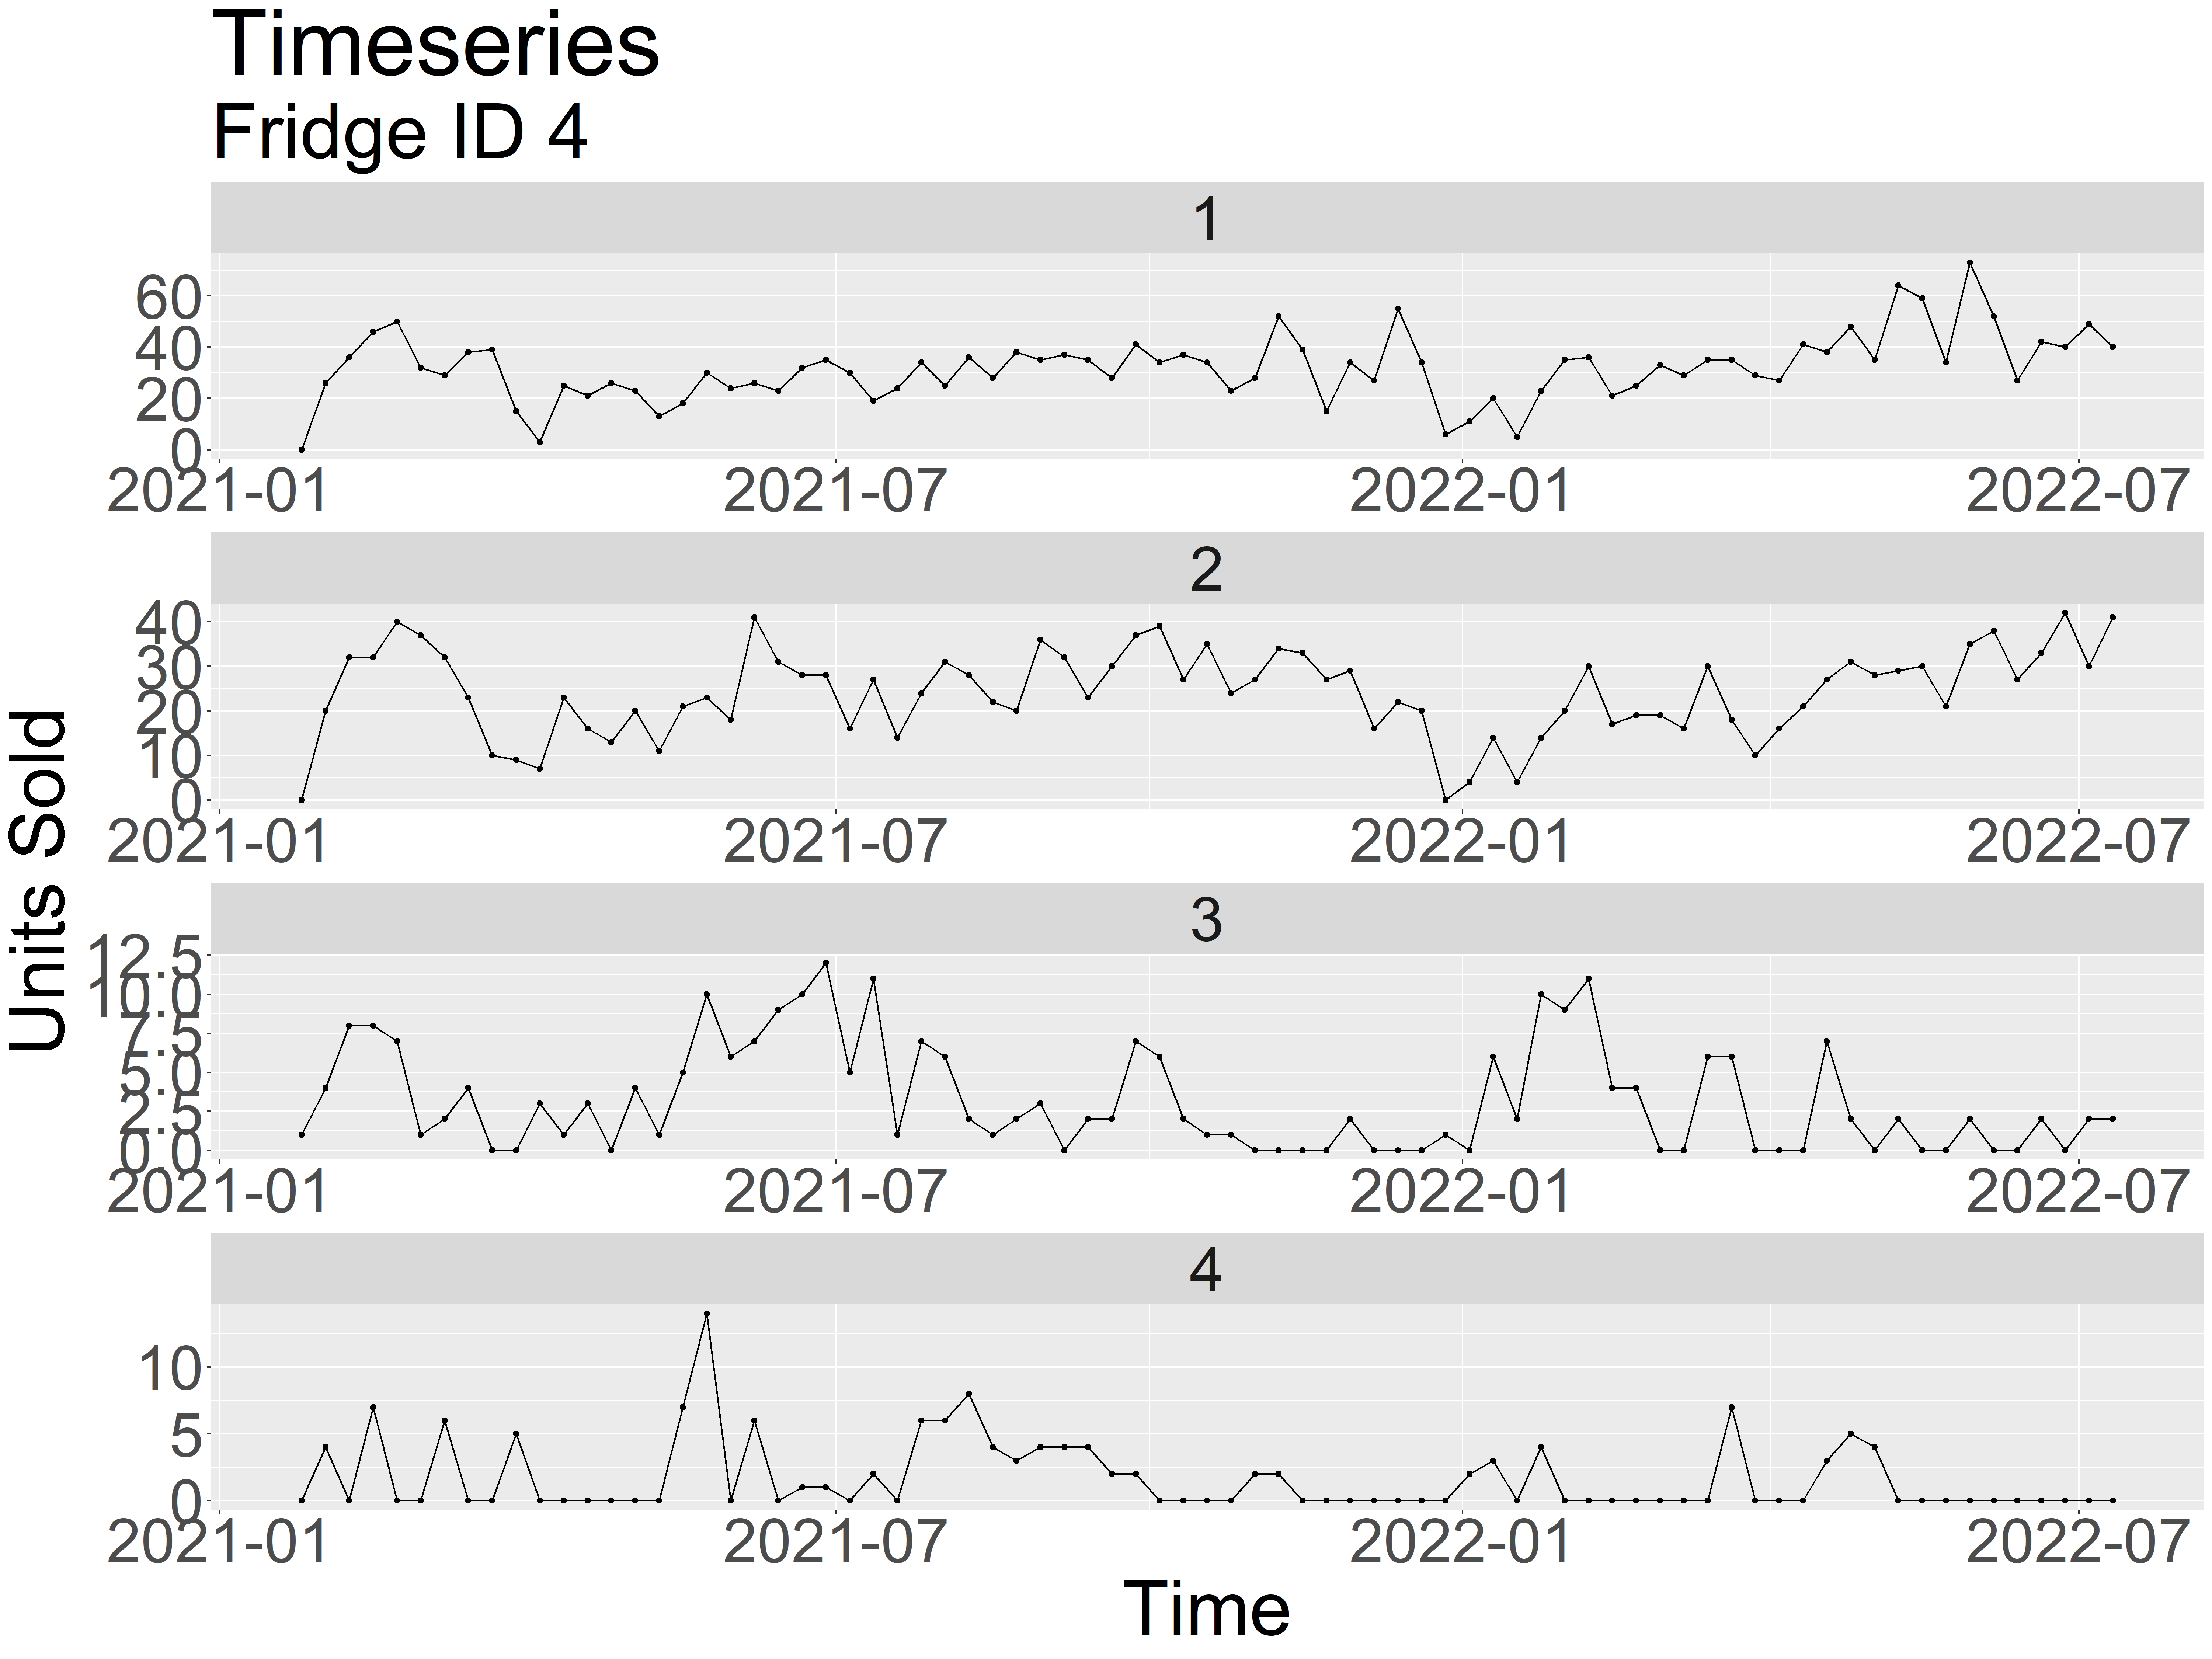
\includegraphics[width=\textwidth]{F:/Uni/Masterarbeit/Master-Thesis_git/Arbeit/Graphiken/Raw_Timeseries_ID4.png}
\caption{Fridge 4 with all four main categories}
\label{fig:TS Fridge 4}
\end{subfigure}
\hfill
\begin{subfigure}[b]{0.45\textwidth}
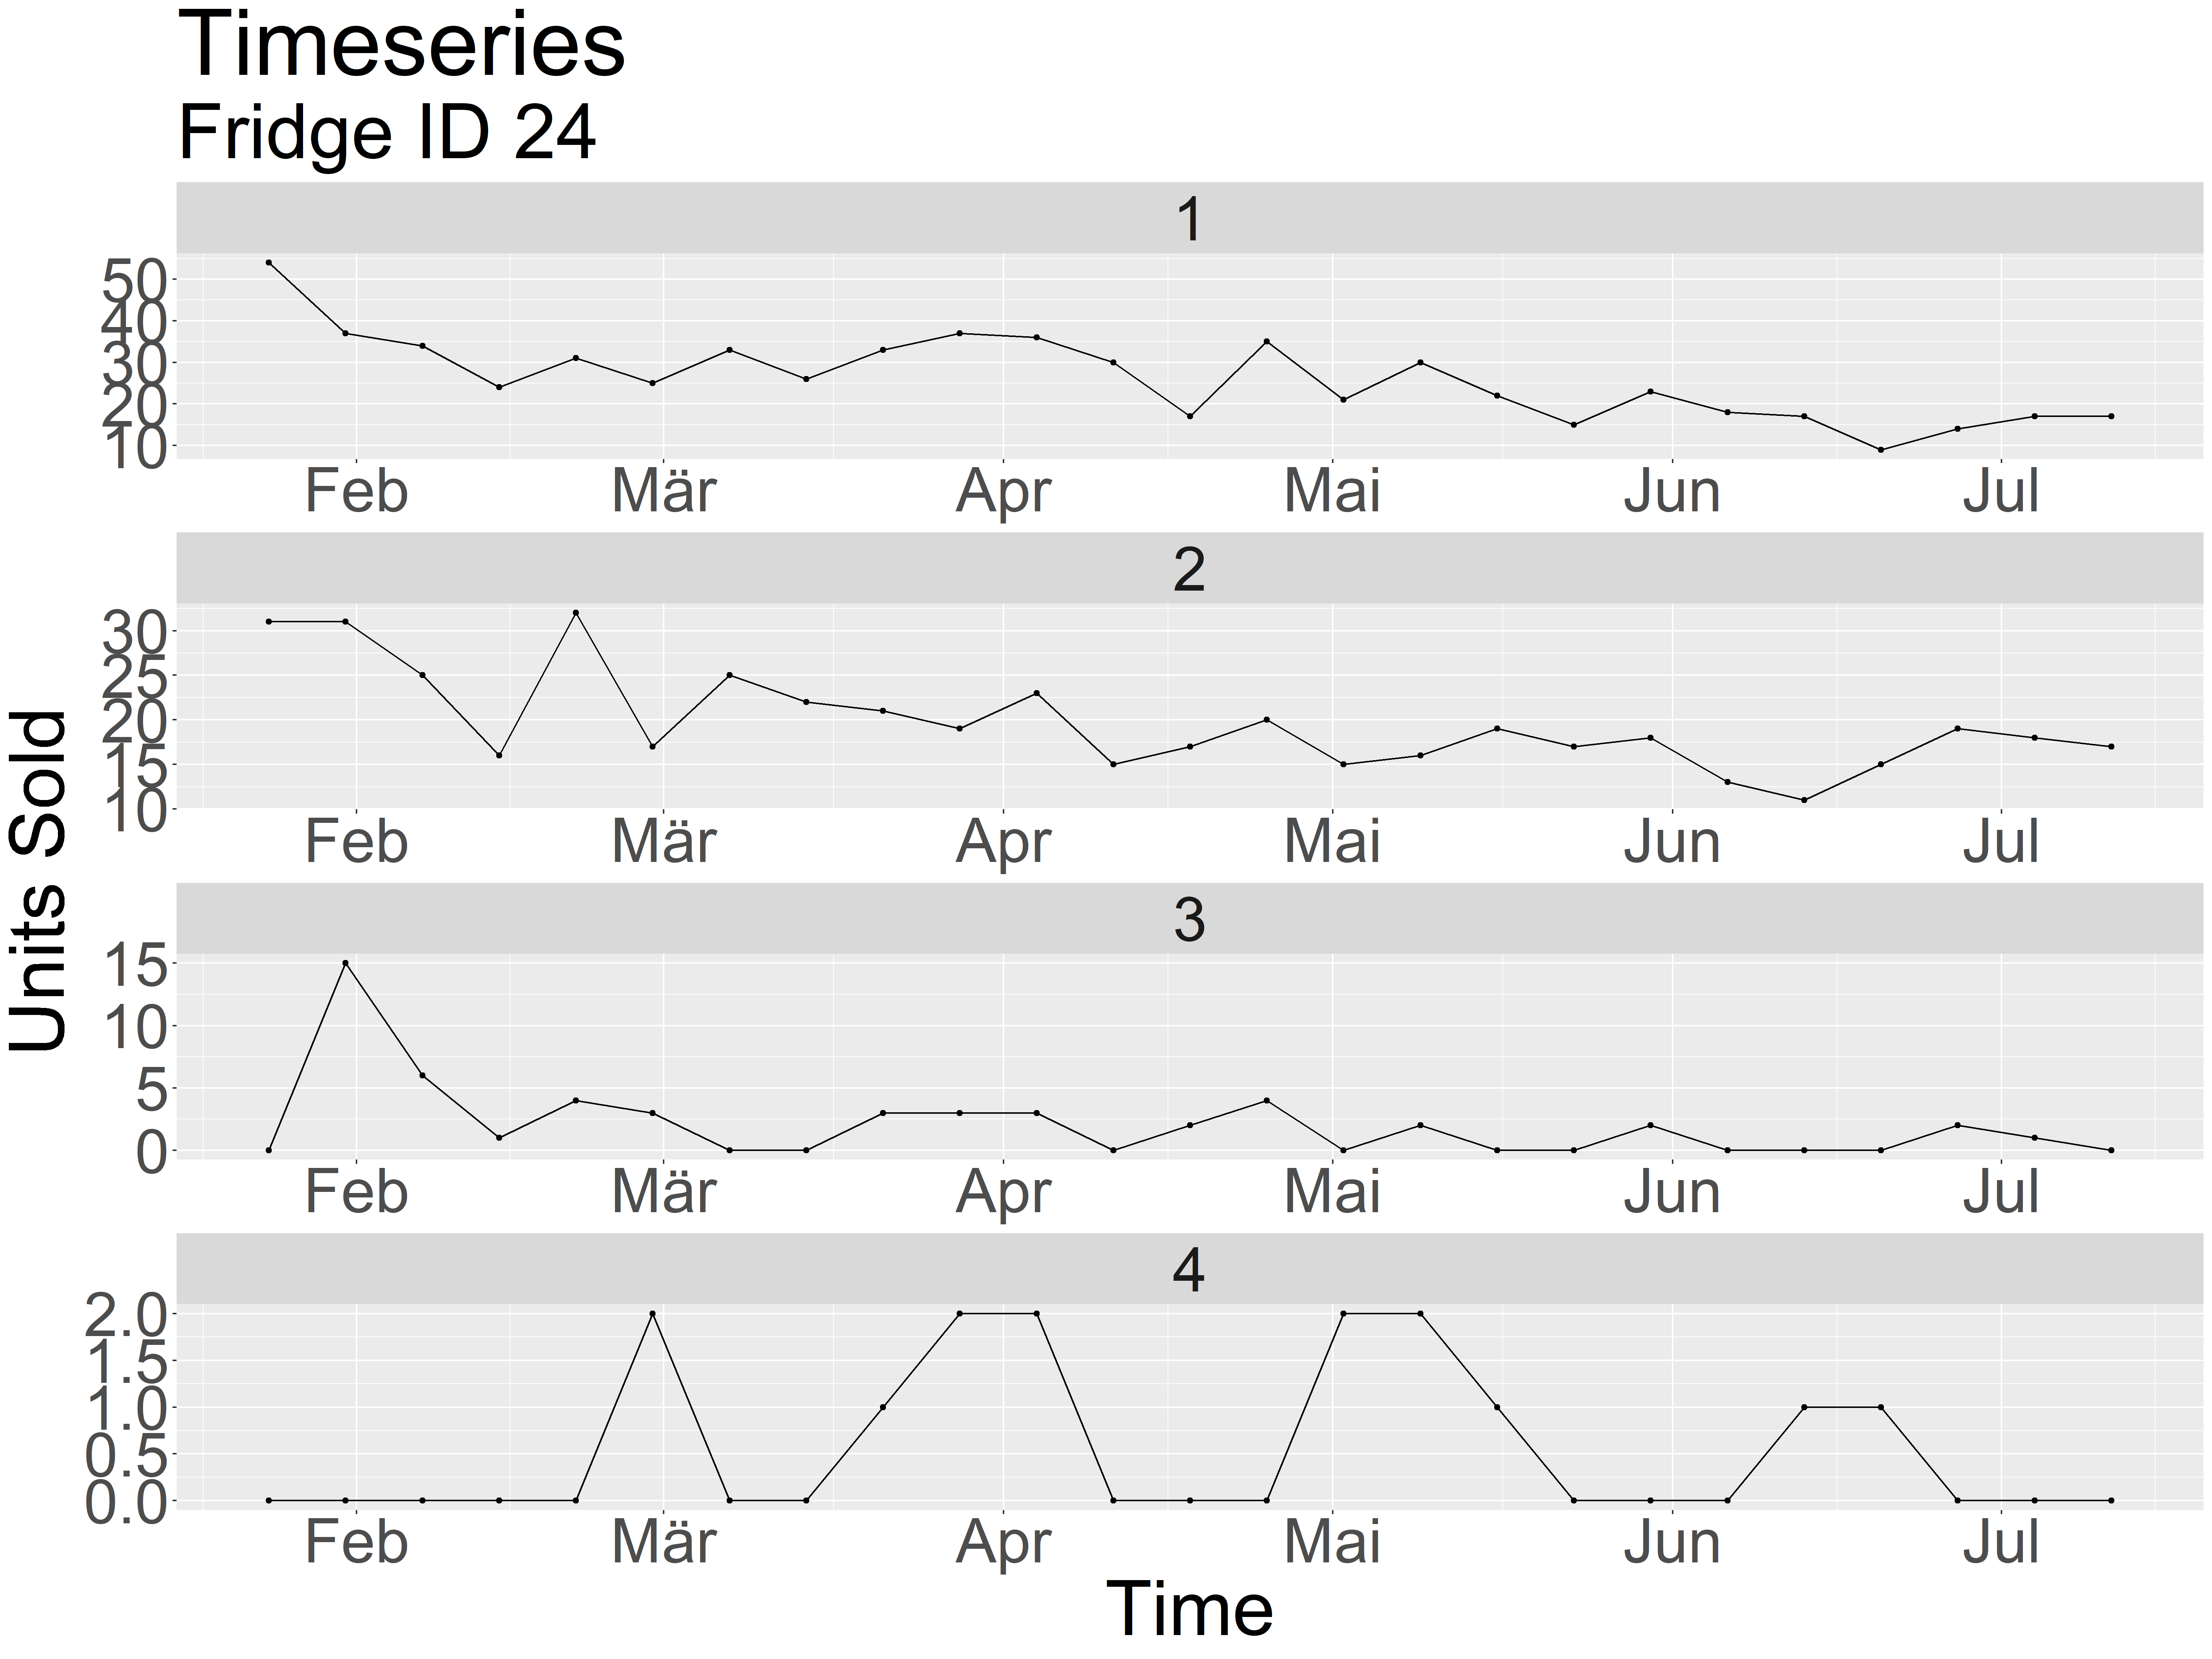
\includegraphics[width=\textwidth]{F:/Uni/Masterarbeit/Master-Thesis_git/Arbeit/Graphiken/Raw_Timeseries_ID24.png}
\caption{Fridge 24 with all four main categories}
\label{fig:TS Fridge 24}
\end{subfigure}
\caption{Timeseries for two fridges}
\label{fig:TS raw}
\end{figure}


The two plots in \ref{fig:TS raw} are good examples of the composition of our data. The scales of the sold units within a fridge vary widely. For example in figure \ref{fig:TS Fridge 24} the values for category 1 vary from above 50 to as low as 10, while for category 4 we only have values in the range of 0 to 2. In both figures \ref{fig:TS raw} for category 4, we can see the excessive amount of zero values in our data which makes the previously mentioned transformations necessary. 

Next in figure \ref{fig:TS Coda}, we add the predictions of the CoDA model. For this model we used the whole history and half of the data for the window length. In addition we extend the window at every time point, add 0.5 to all values and use the one-vs-all method. We can see that this captures the general trend well however, struggles with unexpected high peaks. In addition it is able to handle the difference in scales as seen in \ref{fig:Coda Fridge 4}. Both, categories 1 and 2 with bigger values and categories 3 and 4 with lower values, are in general modelled well. Also in timeseries with less data available, as in fridge 24 \ref{fig:Coda Fridge 24}, the model works well. Especially category 3 with its low values is predicted well. 

\begin{figure}[htb]
\centering
\begin{subfigure}[b]{0.45\textwidth}
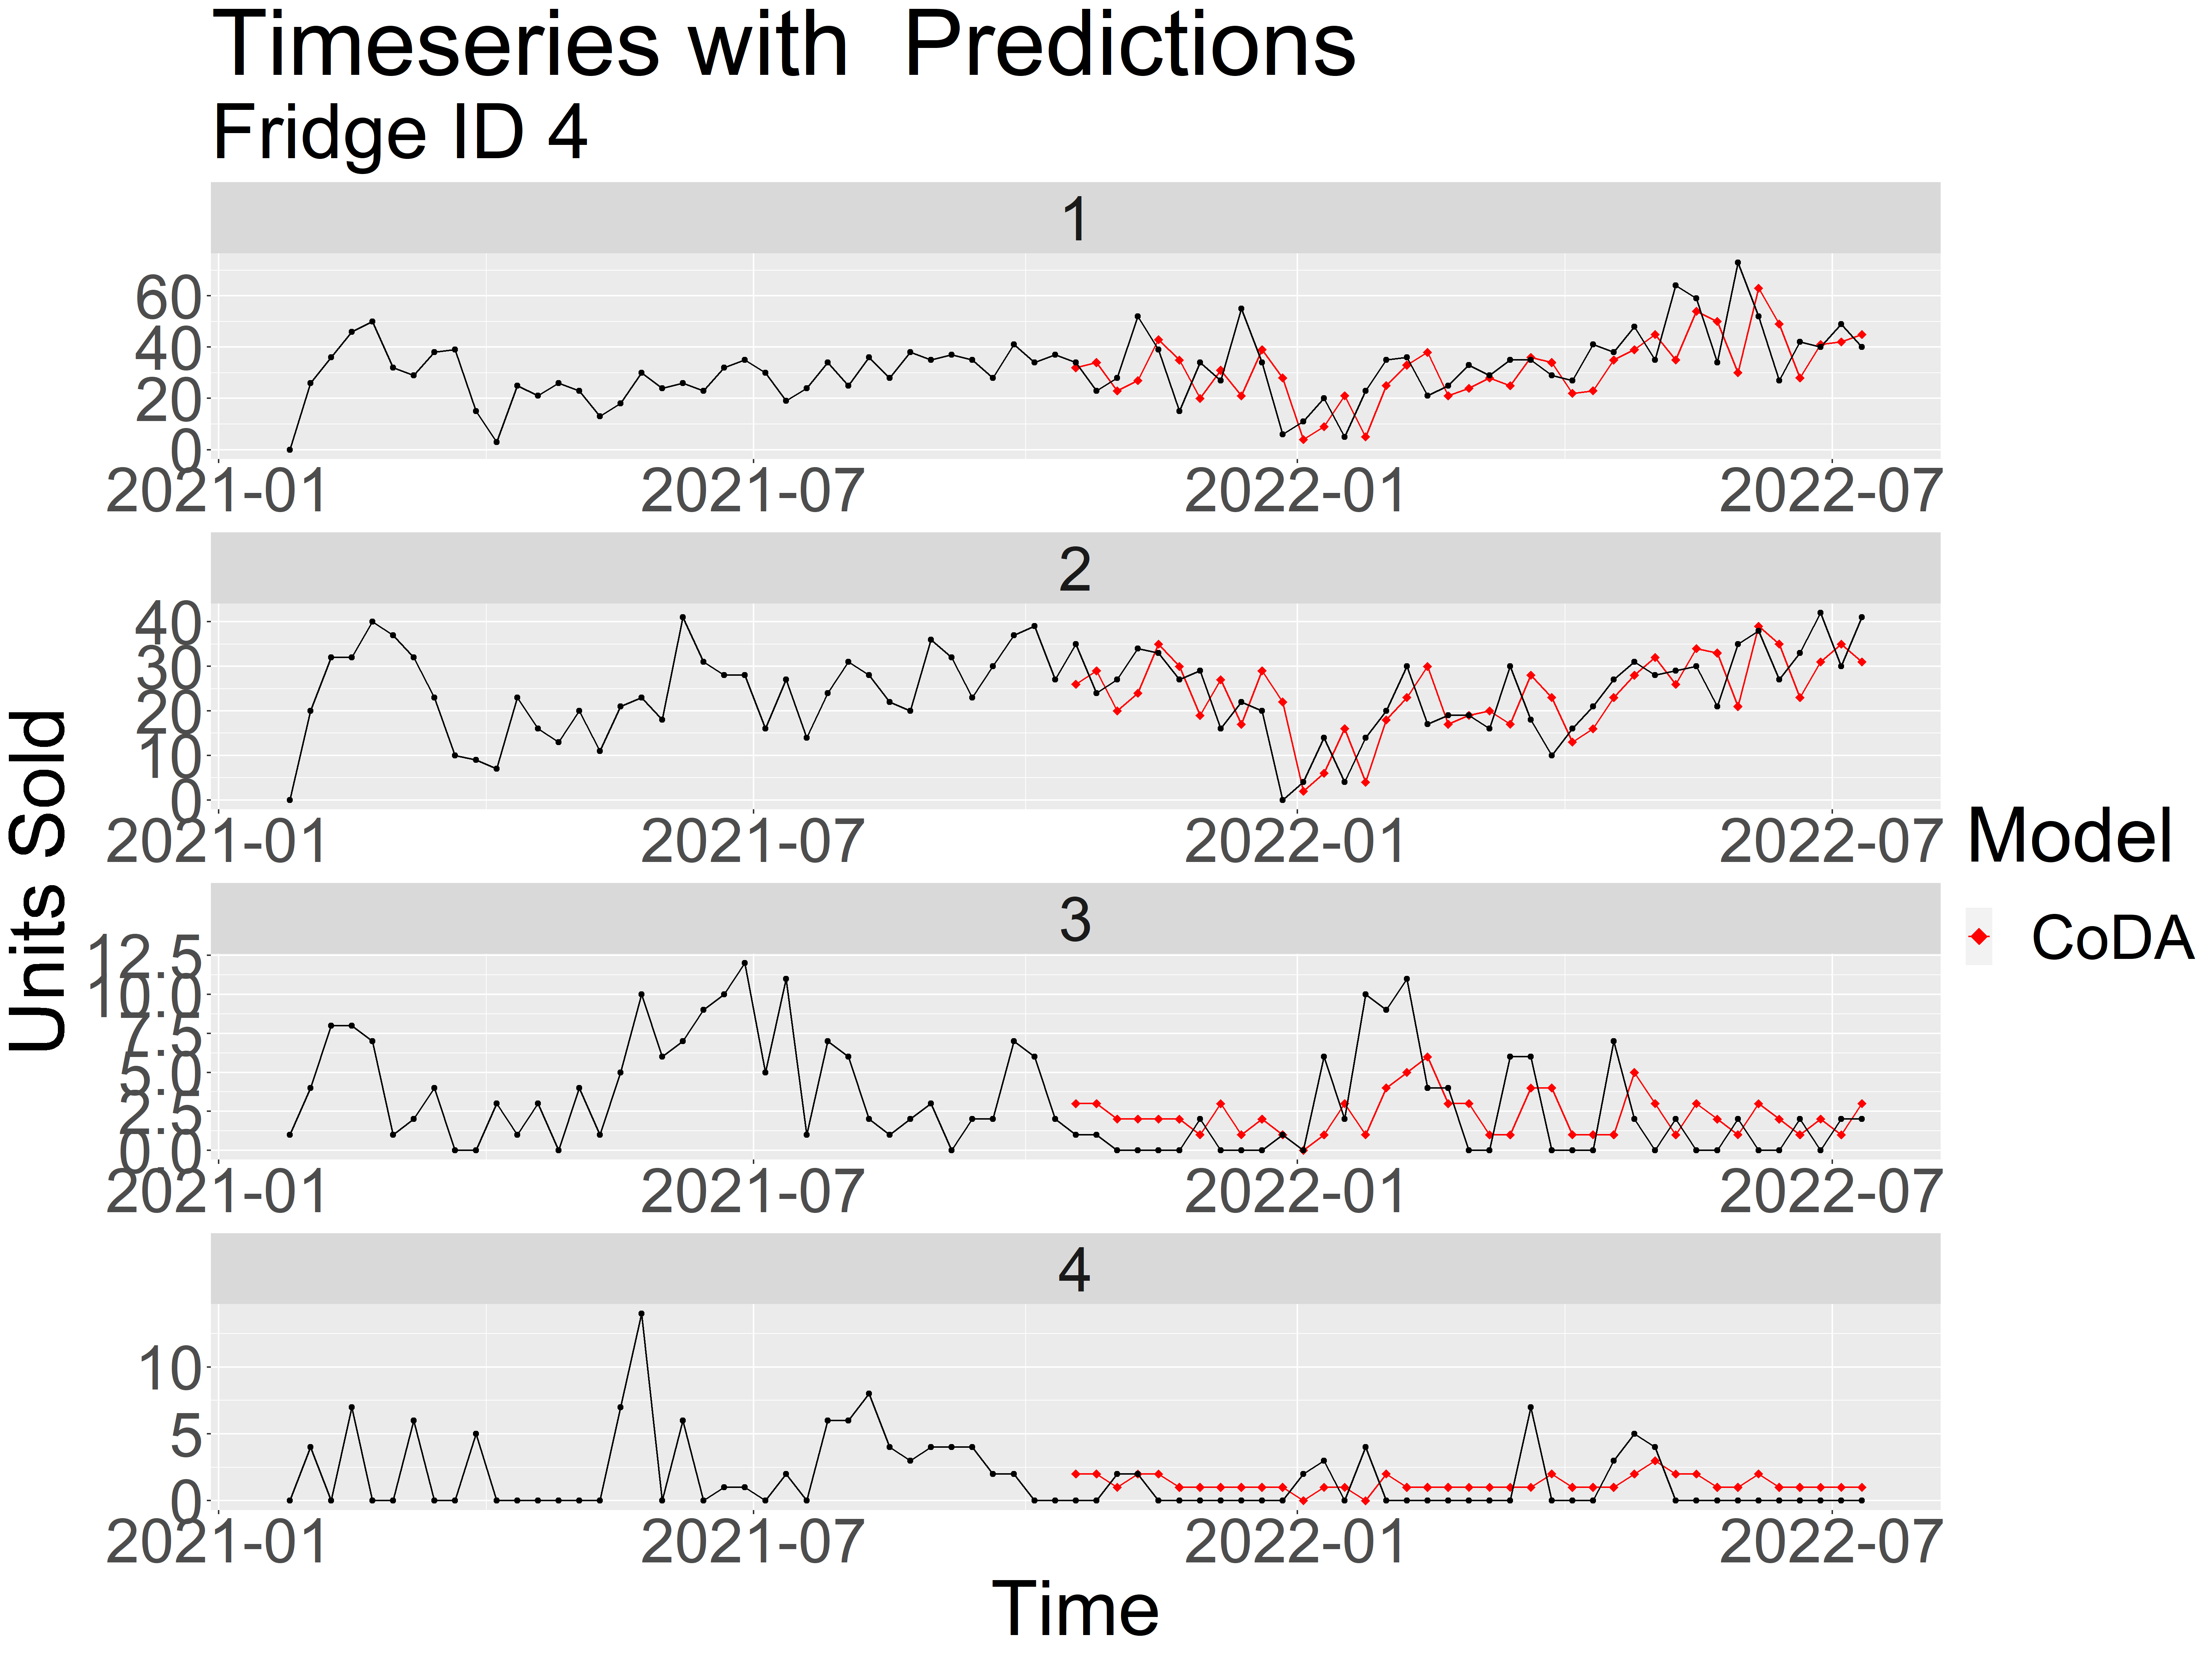
\includegraphics[width=\textwidth]{F:/Uni/Masterarbeit/Master-Thesis_git/Arbeit/Graphiken/Coda_Timeseries_ID4.png}
\caption{Fridge 4 with the CoDA model}
\label{fig:Coda Fridge 4}
\end{subfigure}
\hfill
\begin{subfigure}[b]{0.45\textwidth}
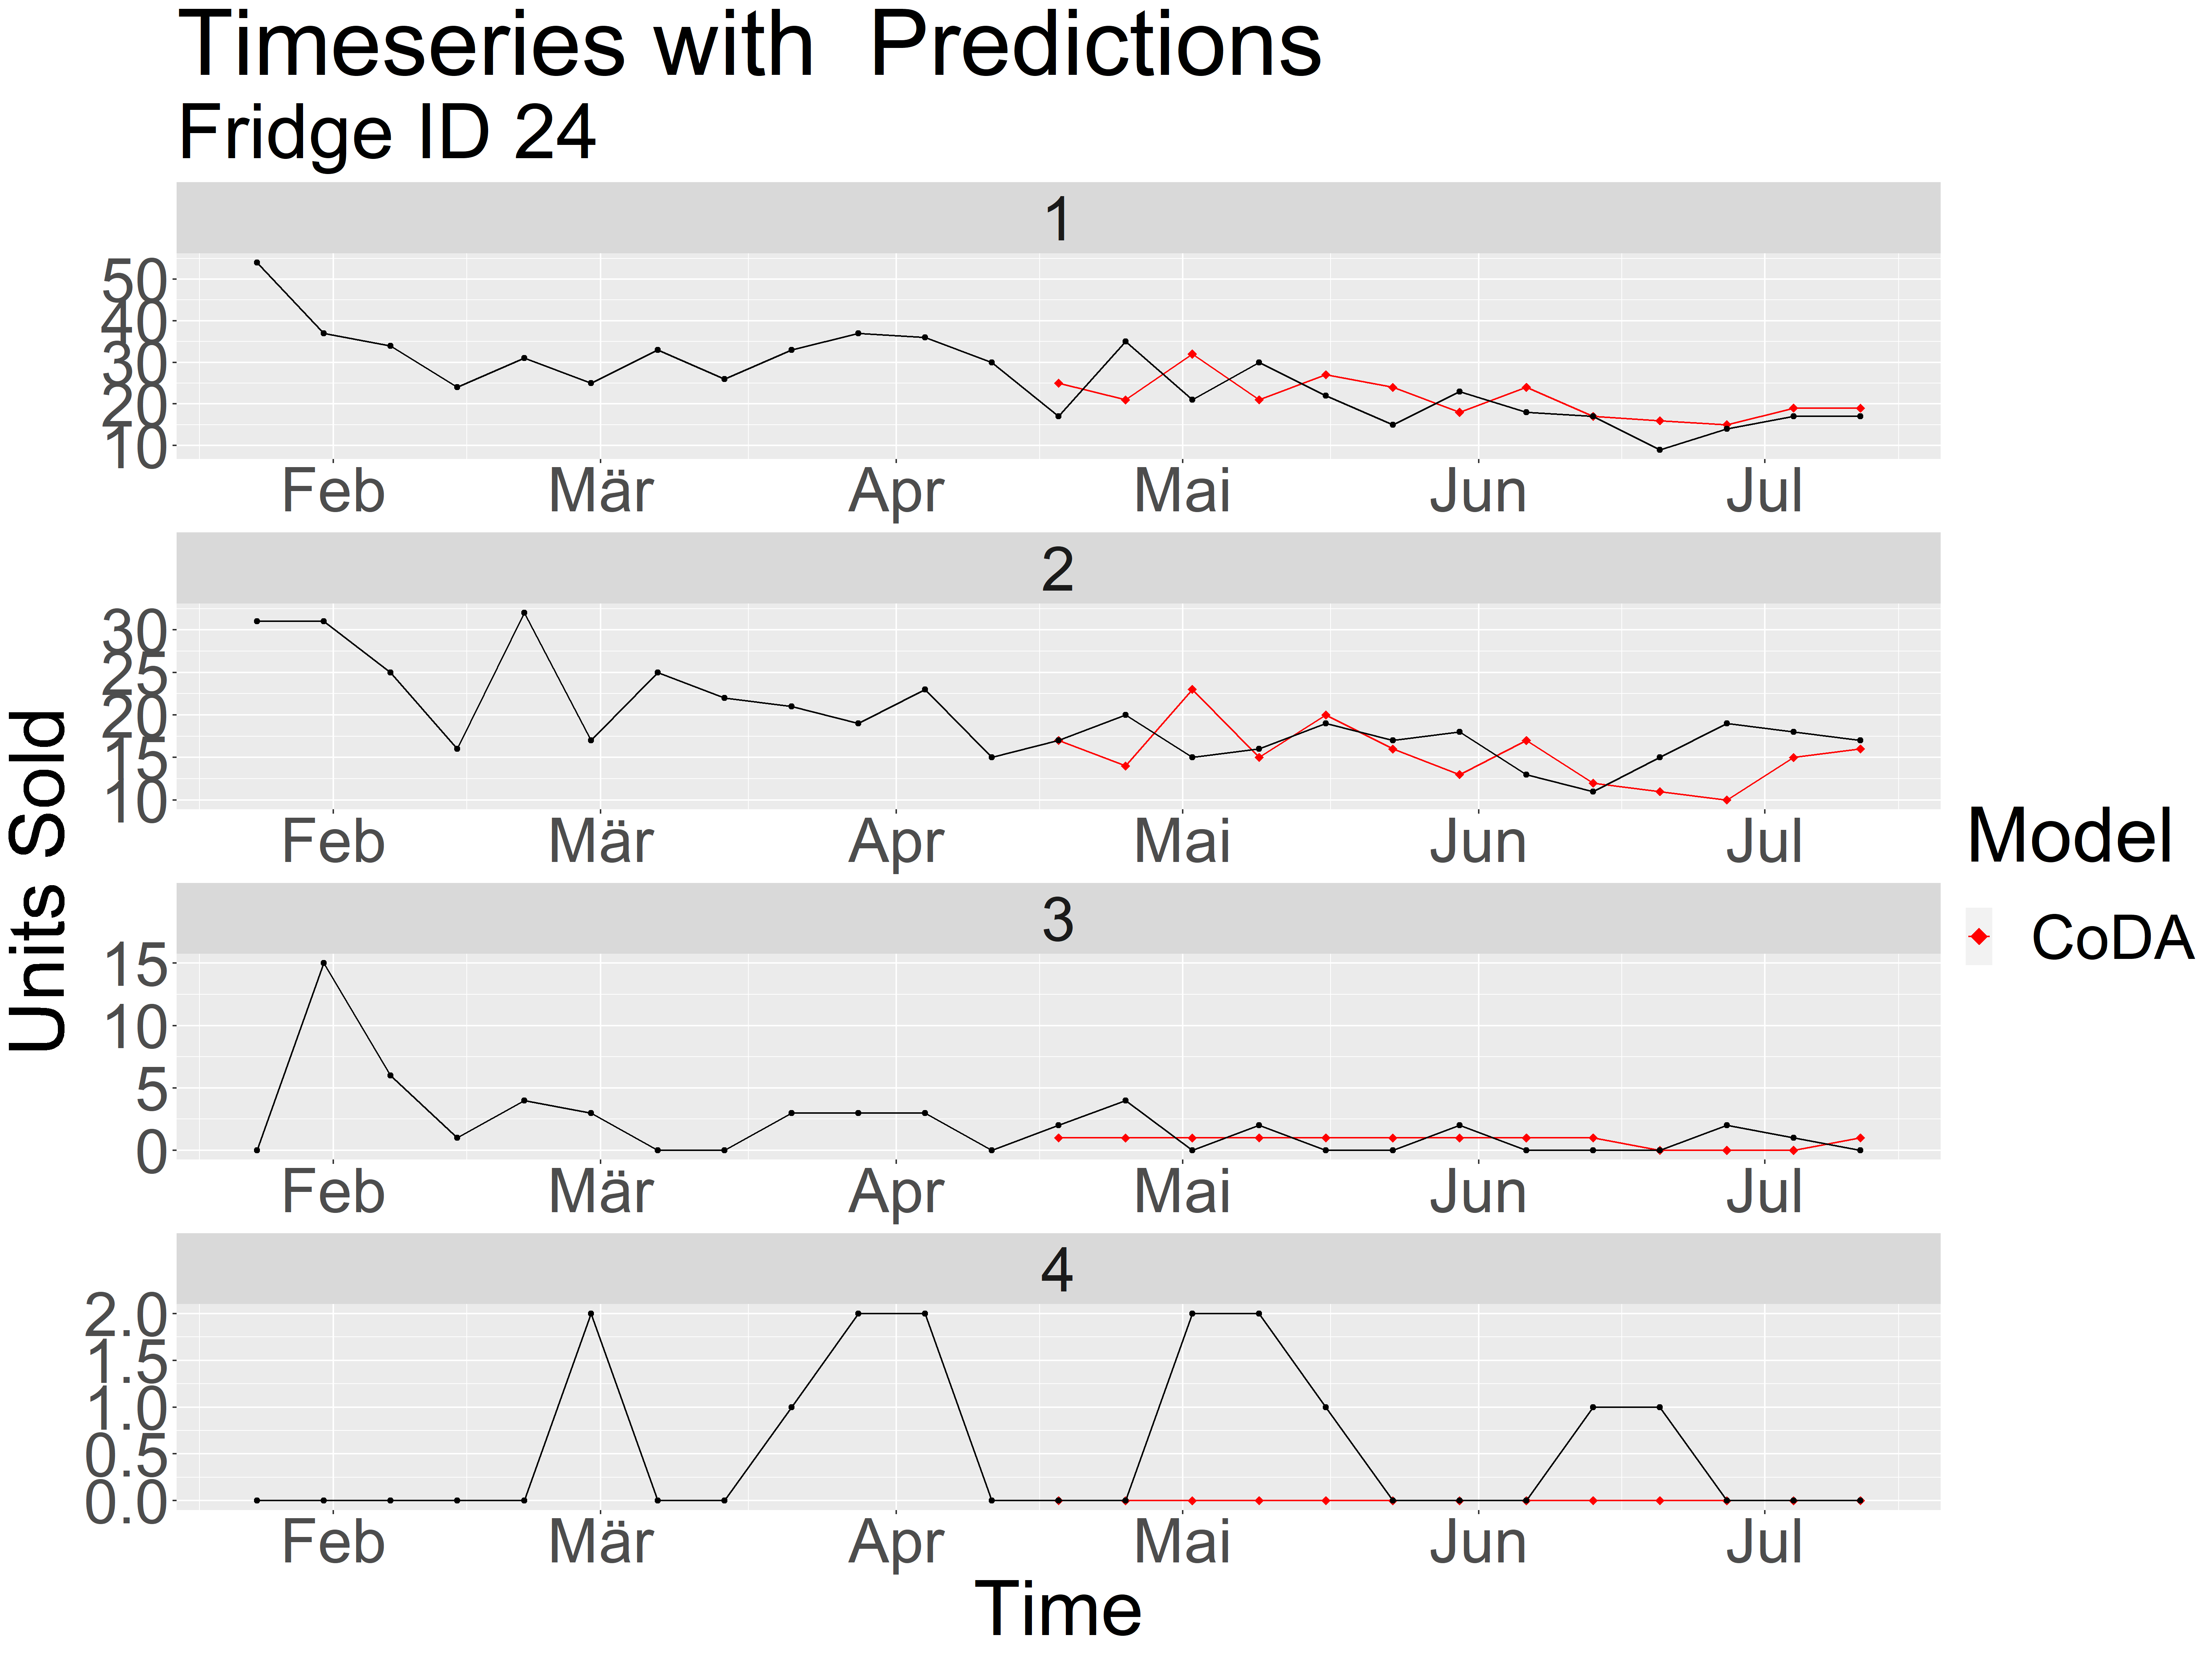
\includegraphics[width=\textwidth]{F:/Uni/Masterarbeit/Master-Thesis_git/Arbeit/Graphiken/Coda_Timeseries_ID24.png}
\caption{Fridge 24 with the CoDA model}
\label{fig:Coda Fridge 24}
\end{subfigure}
\caption{Timeseries with CoDA model}
\label{fig:TS Coda}
\end{figure}



In figure \ref{fig:TS Ingarch} we apply the INGARCH model to the timeseries. For this, we used the whole history, half of the data for the window length, extend the window at every time point, add one to all zero values and used the poisson distribution. We used no external factors and set $p=1, q=1$ in model \ref{eq:Ingarch model with external effect}. The general trend is again captured well and in the instance of \ref{fig:Ingarch Fridge 4} it seems to be more reactive to sudden peaks, as often the value predicted after such a peak is heavily influenced by it.

\begin{figure}[htb]
\centering
\begin{subfigure}[b]{0.45\textwidth}
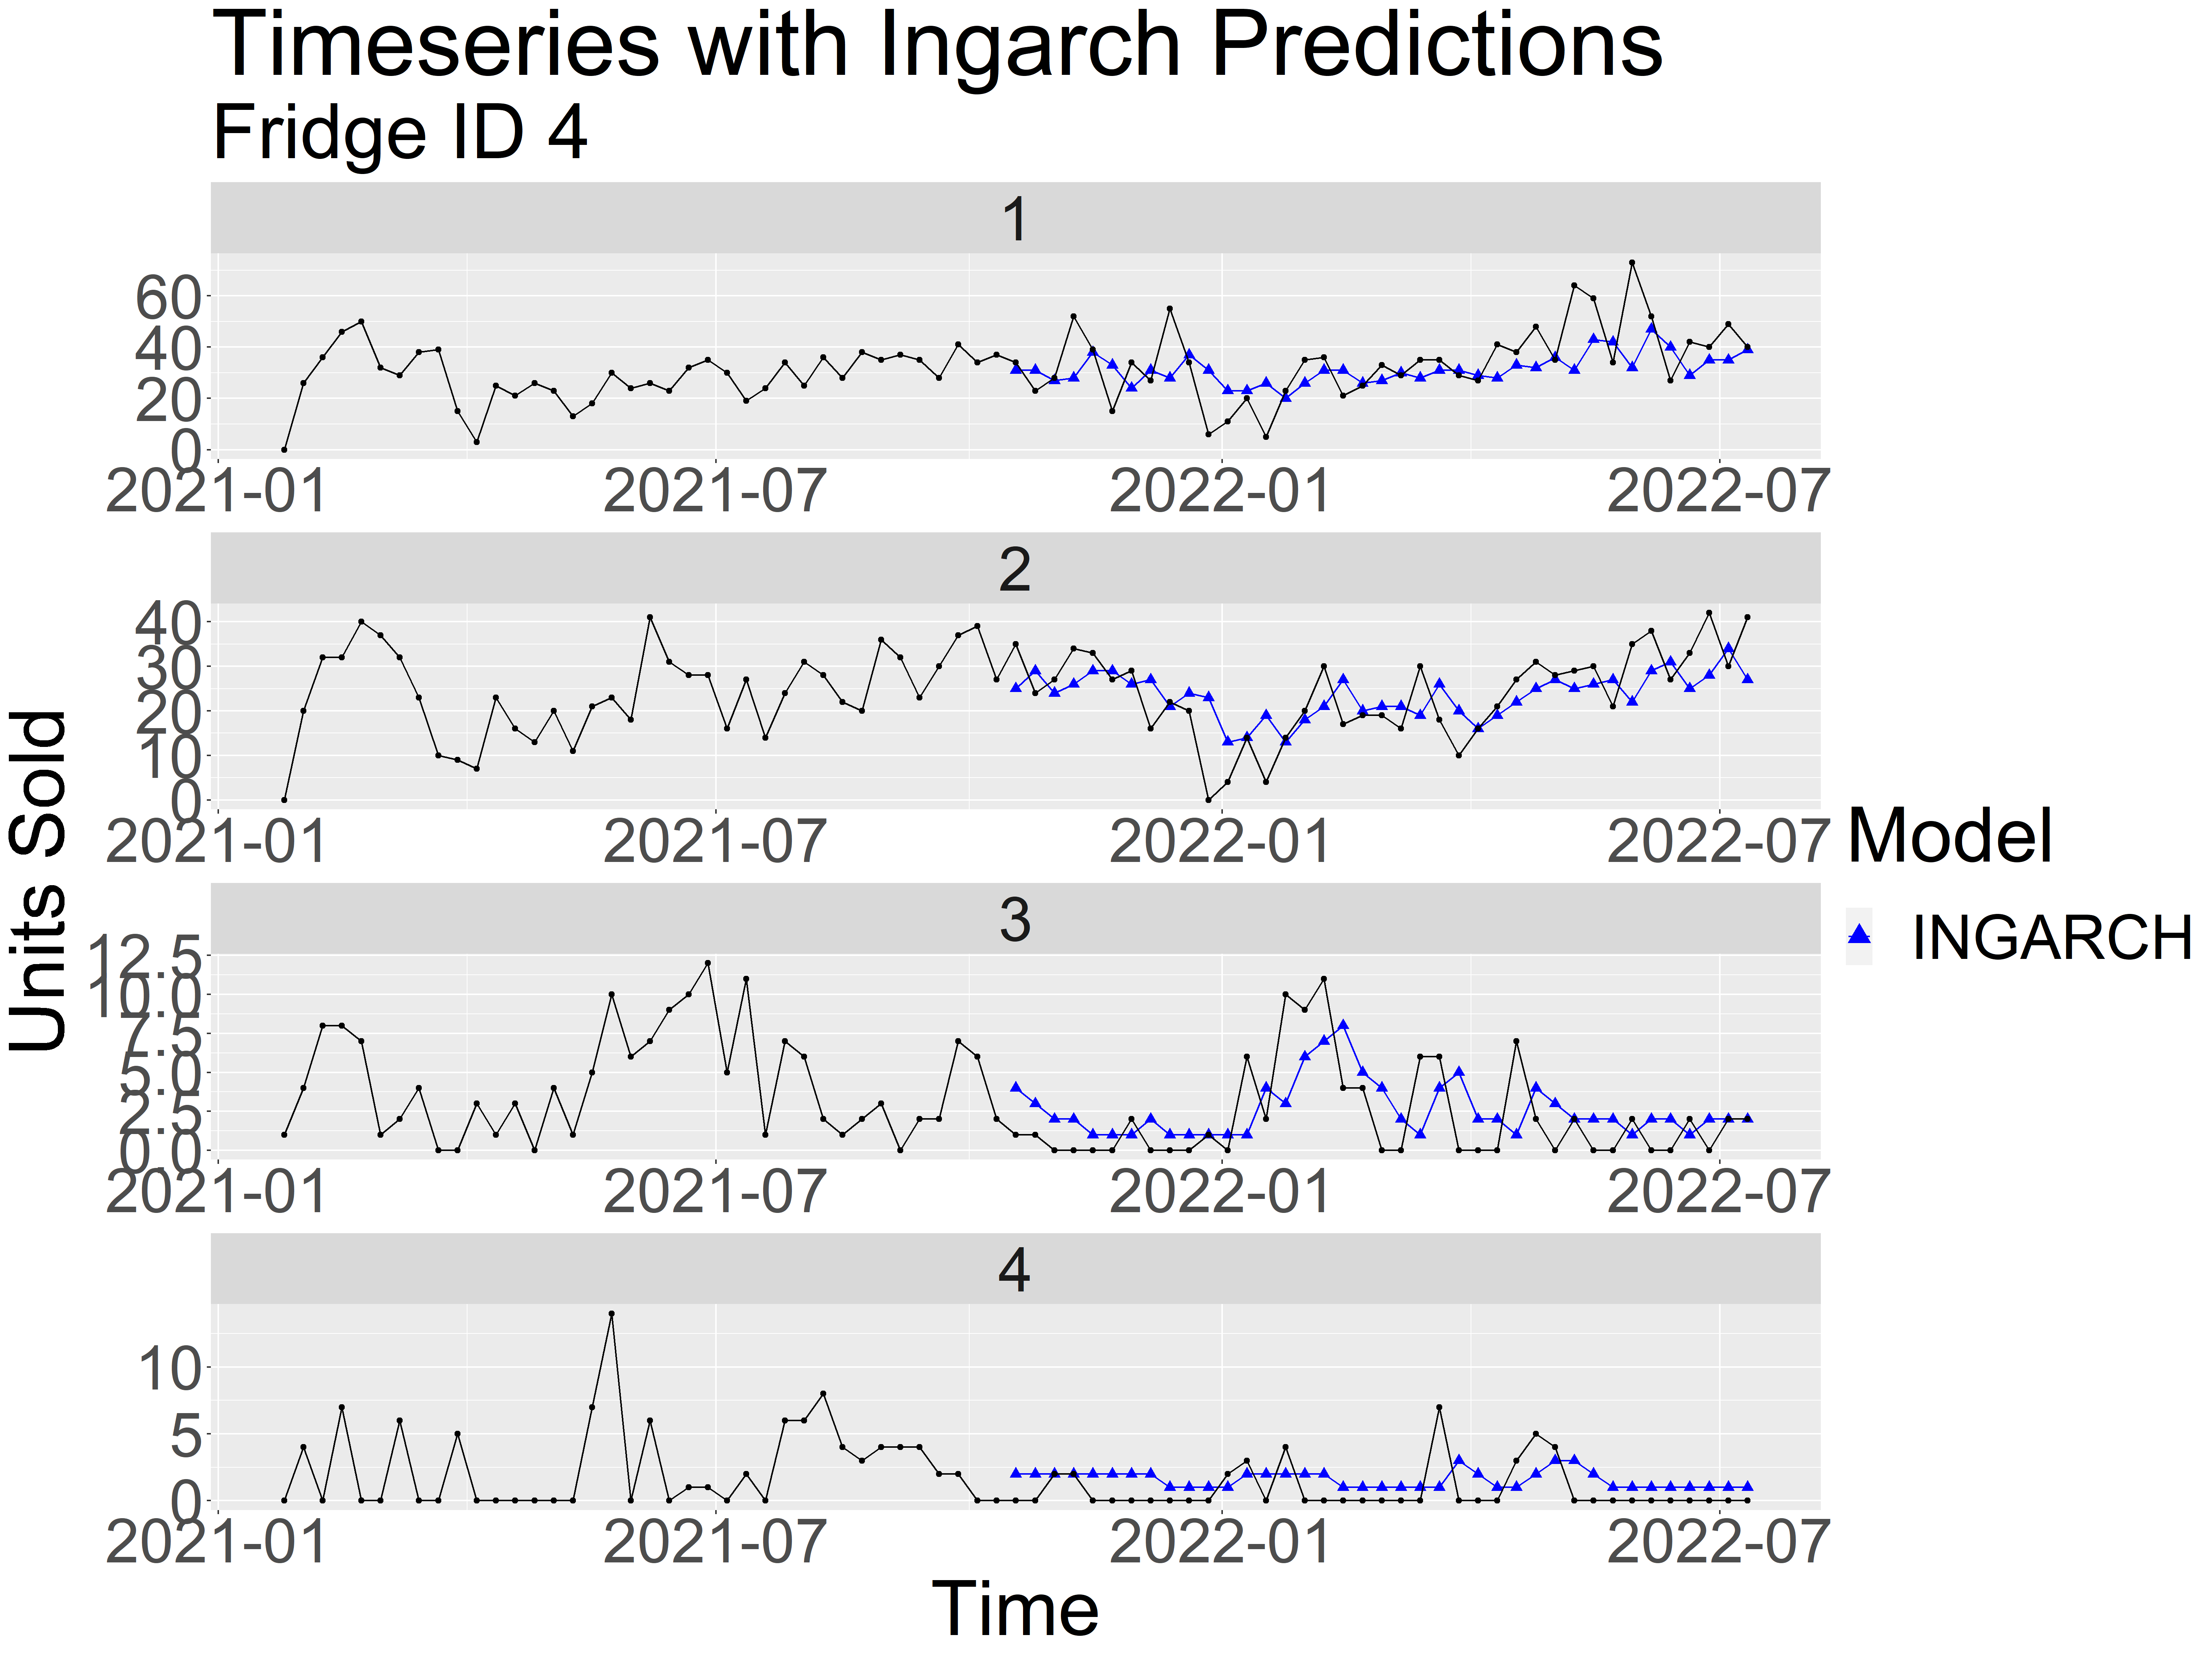
\includegraphics[width=\textwidth]{F:/Uni/Masterarbeit/Master-Thesis_git/Arbeit/Graphiken/Ingarch_Timeseries_ID4.png}
\caption{Fridge 4 with the INGARCH model}
\label{fig:Ingarch Fridge 4}
\end{subfigure}
\hfill
\begin{subfigure}[b]{0.45\textwidth}
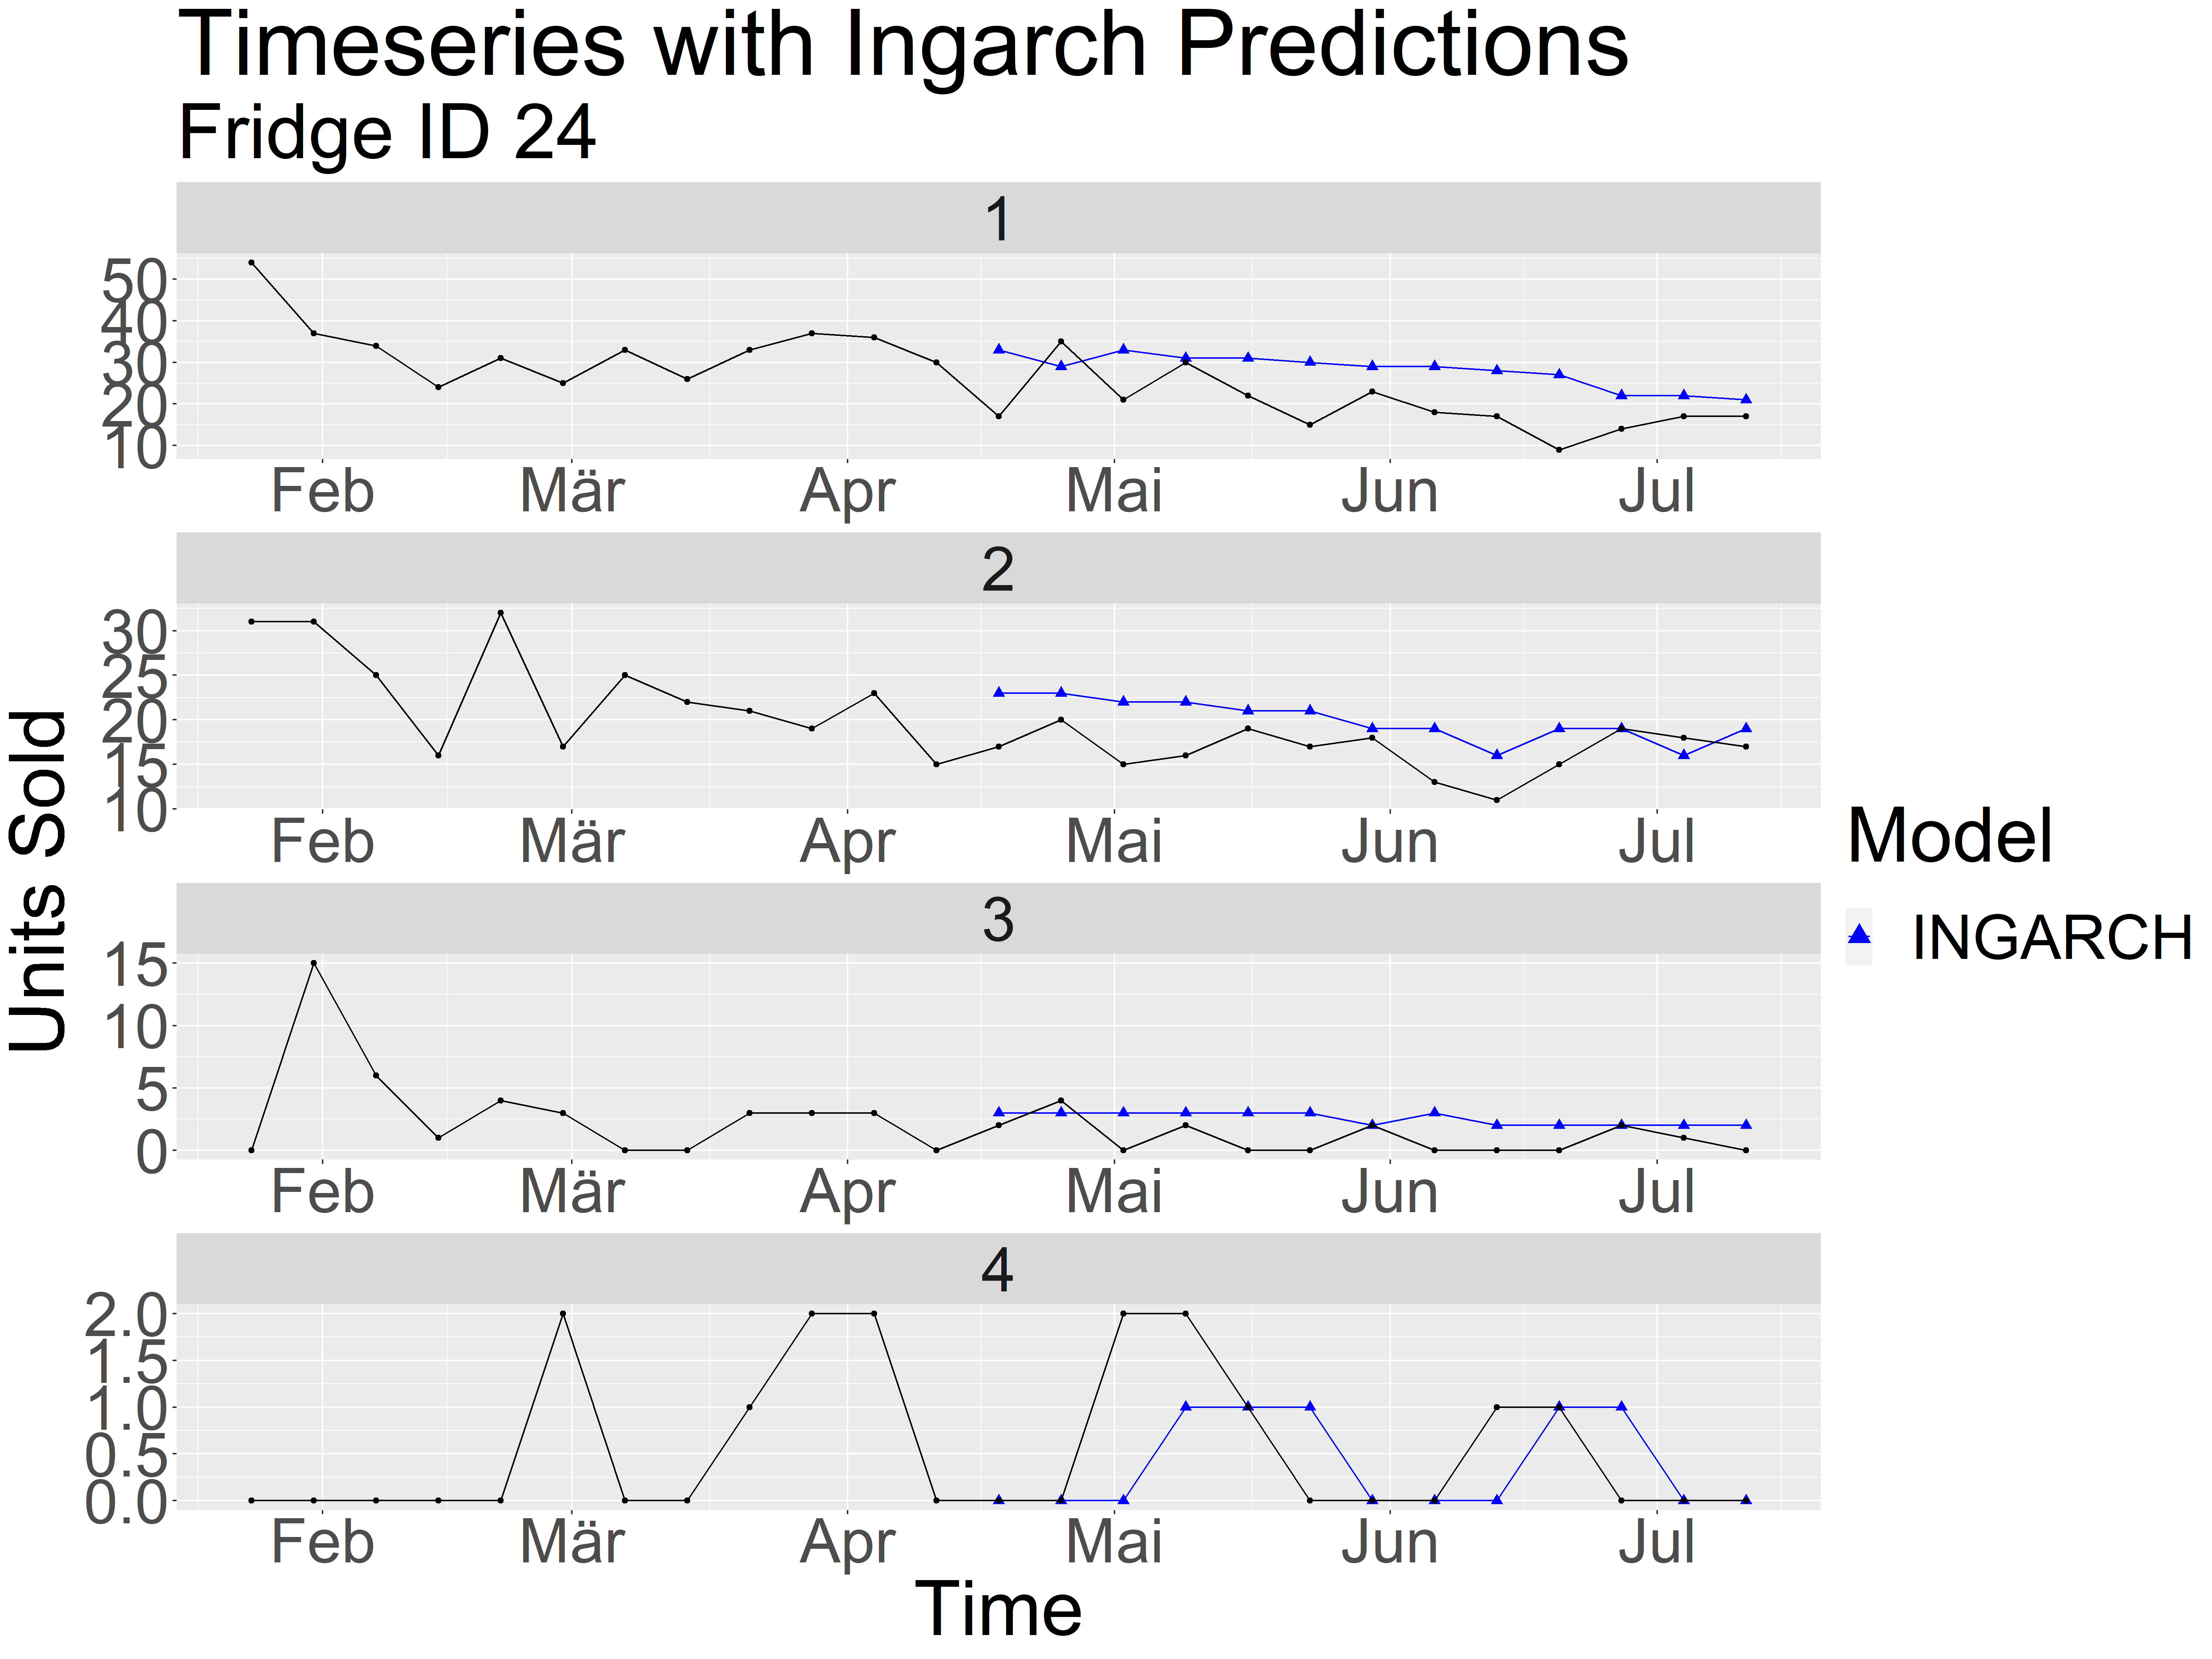
\includegraphics[width=\textwidth]{F:/Uni/Masterarbeit/Master-Thesis_git/Arbeit/Graphiken/Ingarch_Timeseries_ID24.png}
\caption{Fridge 24 with the INGARCH model}
\label{fig:Ingarch Fridge 24}
\end{subfigure}
\caption{Timeseries with INGARCH model}
\label{fig:TS Ingarch}
\end{figure}


To directly compare both models, we plot the predictions in one figure \ref{fig:TS Both}. The model specifications are the same as above. We can see that the models produce similar results to each other. In this instances it appears that INGARCH predicts slightly higher values than CoDA. 

\begin{figure}[htb]
\centering
\begin{subfigure}[b]{0.8\textwidth}
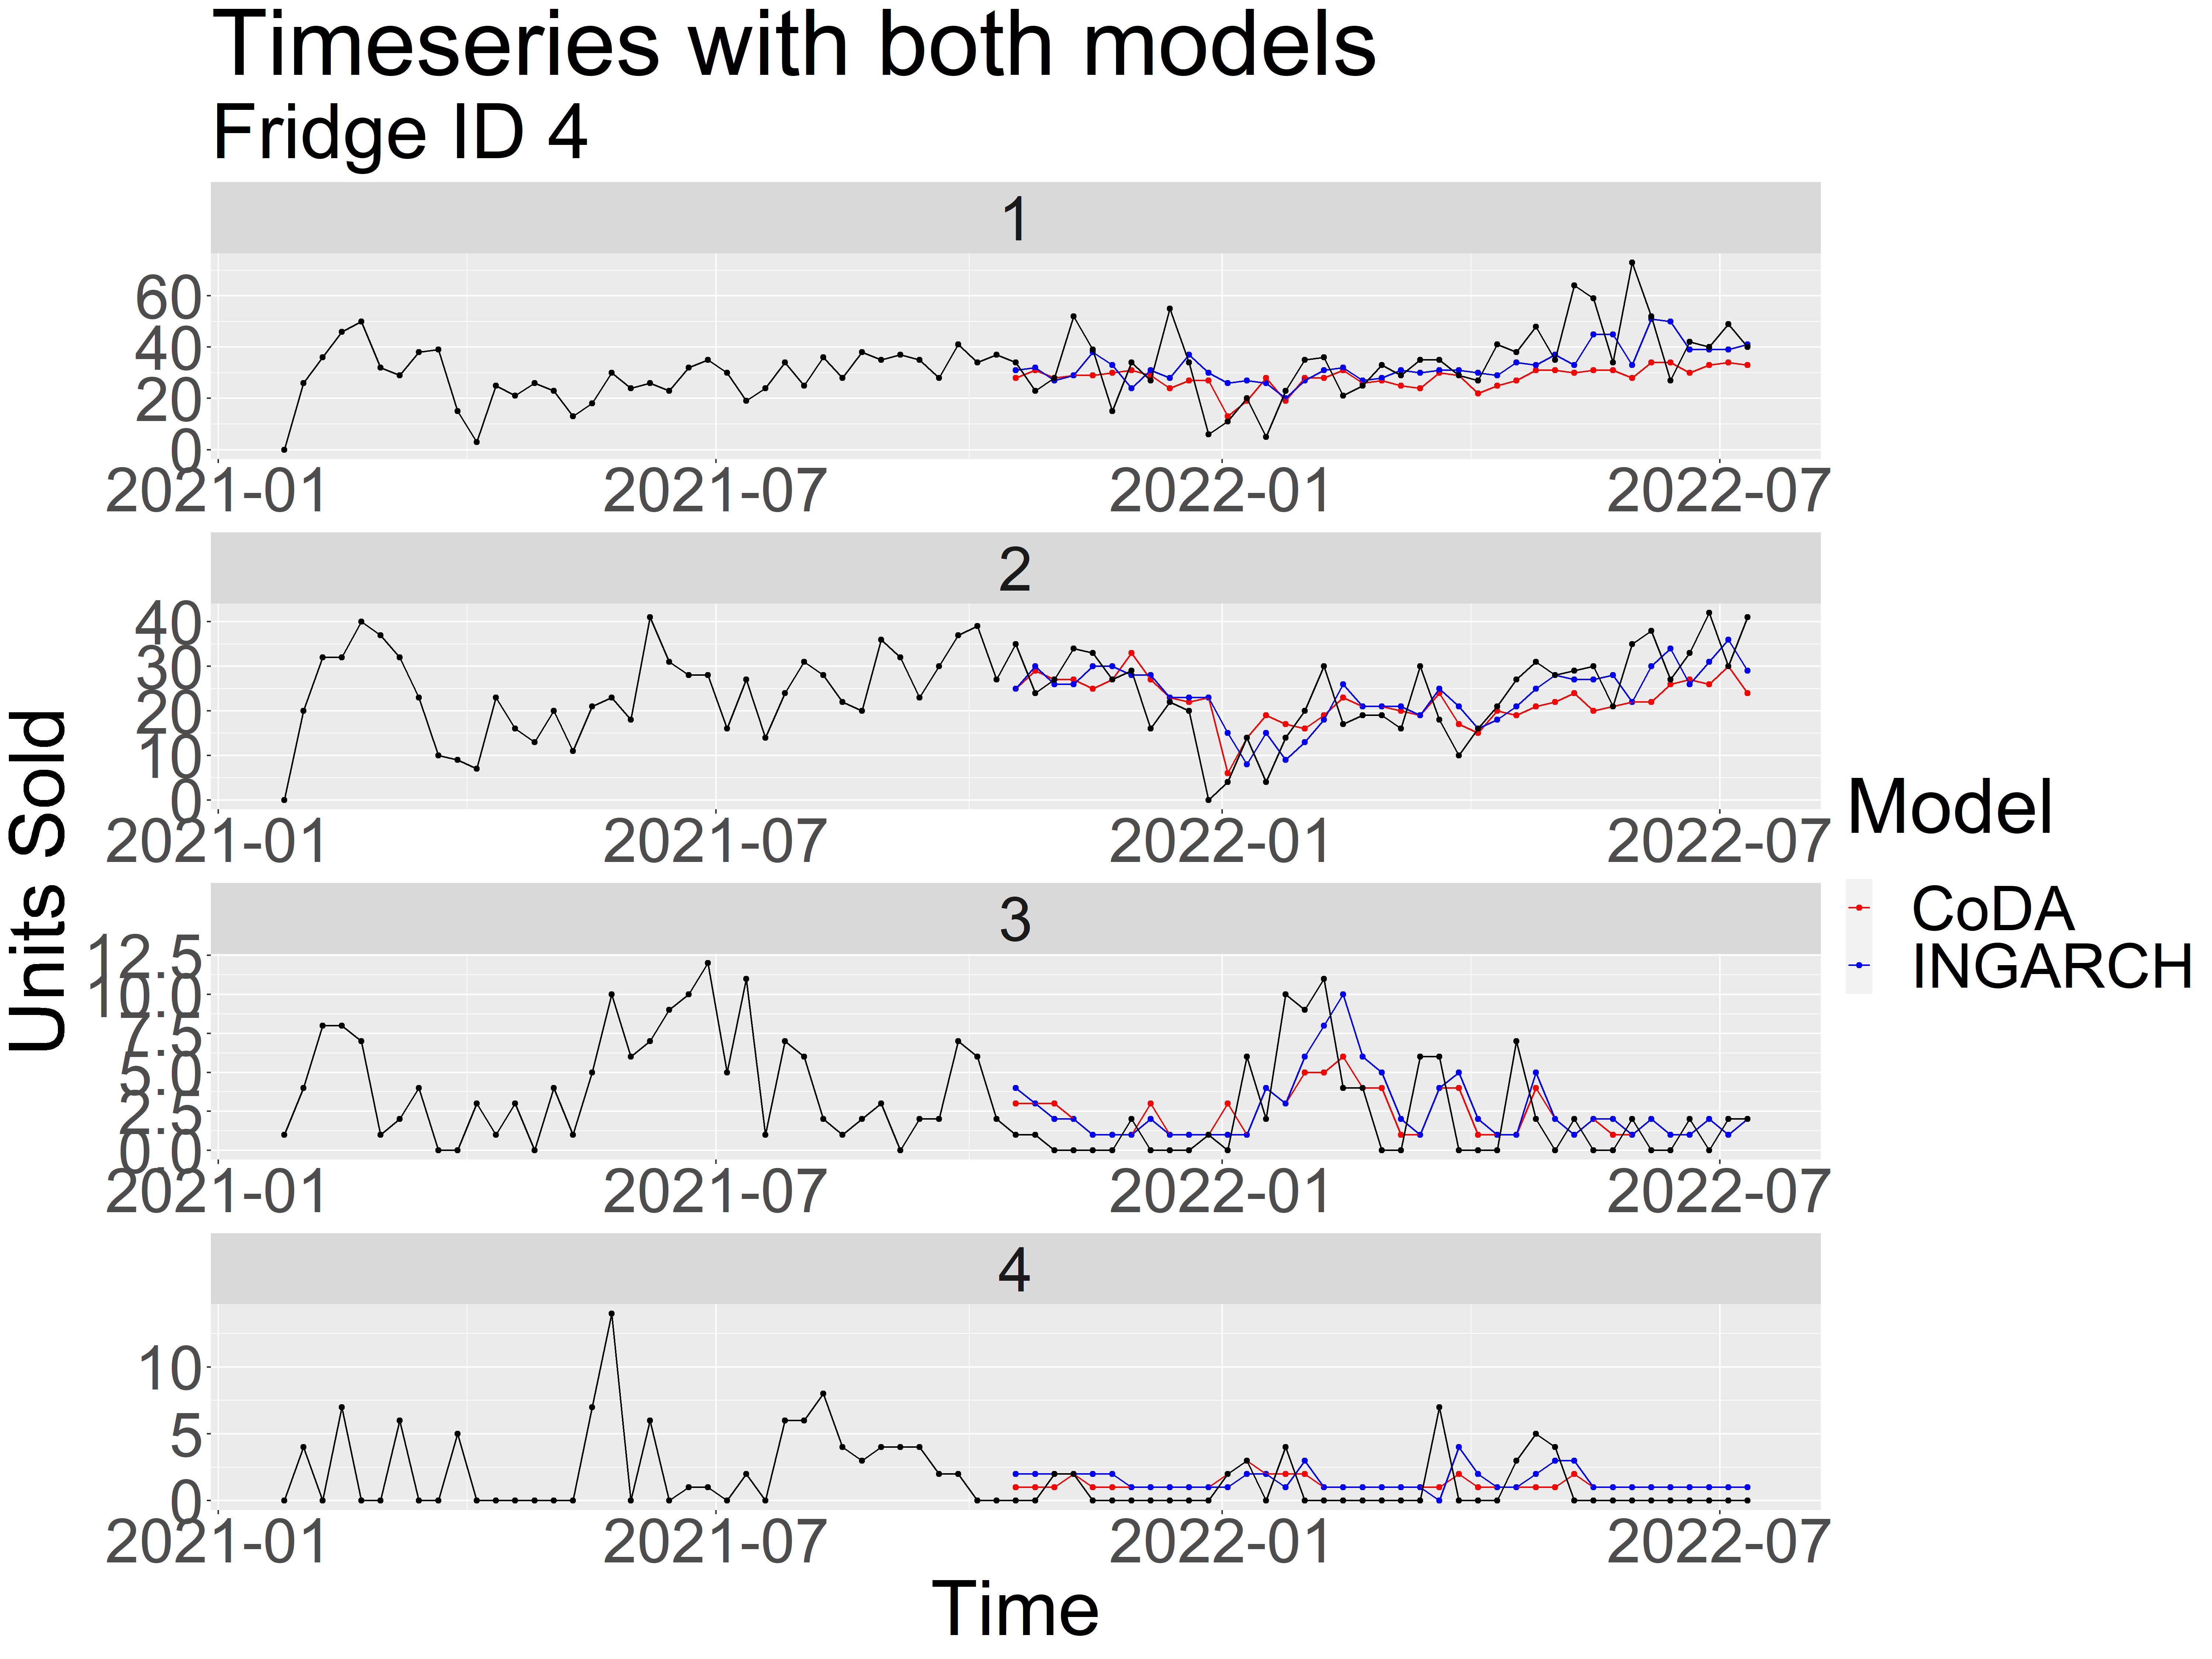
\includegraphics[width=\textwidth]{F:/Uni/Masterarbeit/Master-Thesis_git/Arbeit/Graphiken/Both_Timeseries_ID4.png}
\caption{Fridge 4 with the both models}
\label{fig:Both Fridge 4}
\end{subfigure}
\hfill
\begin{subfigure}[b]{0.8\textwidth}
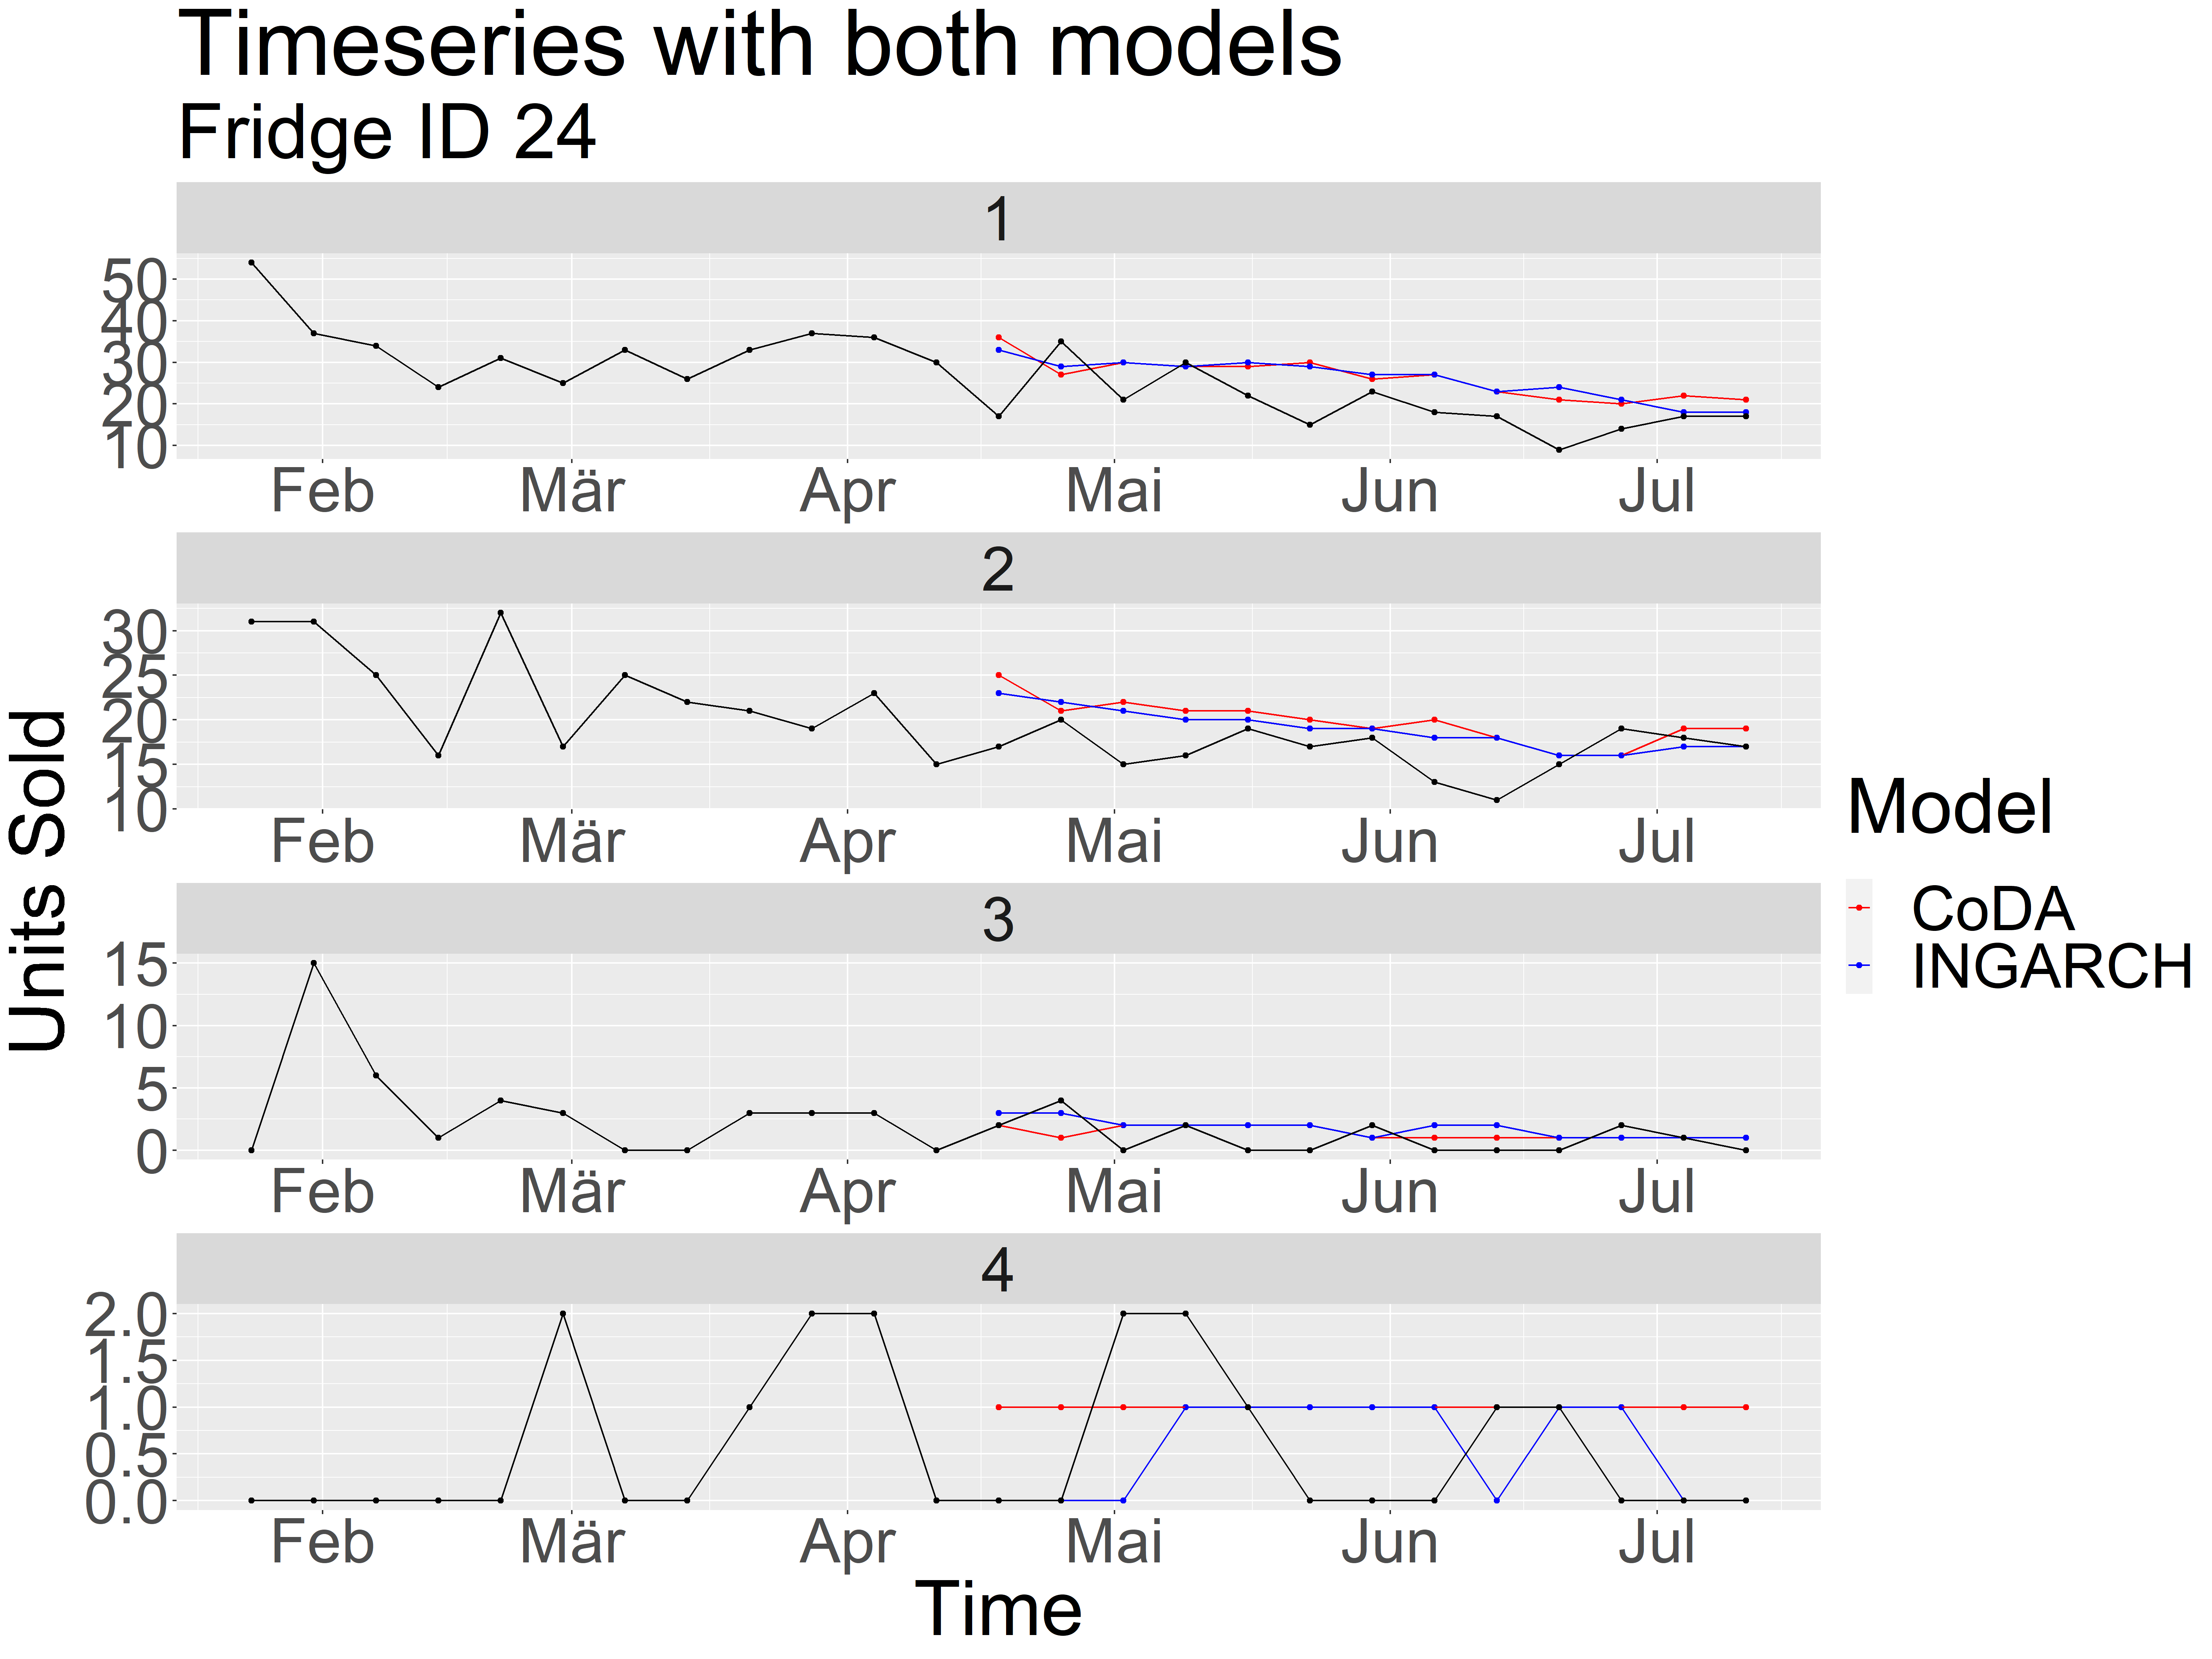
\includegraphics[width=\textwidth]{F:/Uni/Masterarbeit/Master-Thesis_git/Arbeit/Graphiken/Both_Timeseries_ID24.png}
\caption{Fridge 24 with the both models}
\label{fig:Both Fridge 24}
\end{subfigure}
\caption{Timeseries with both models}
\label{fig:TS Both}
\end{figure}


In order to get some further insight in the accuracy of our predictions, we added 95 \% prediction intervals \ref{fig:TS BothPI}. Here we can see some differences between the intervals. While for categories with bigger values the bands are quite similar in width, for categories with lower values, CoDA has much wider bands. This is especially visible in \ref{fig:BothPI Fridge 4} for category 3 and 4. However, most data points are covered by both bands.
\begin{figure}[htb]
\centering
\begin{subfigure}[b]{0.8\textwidth}
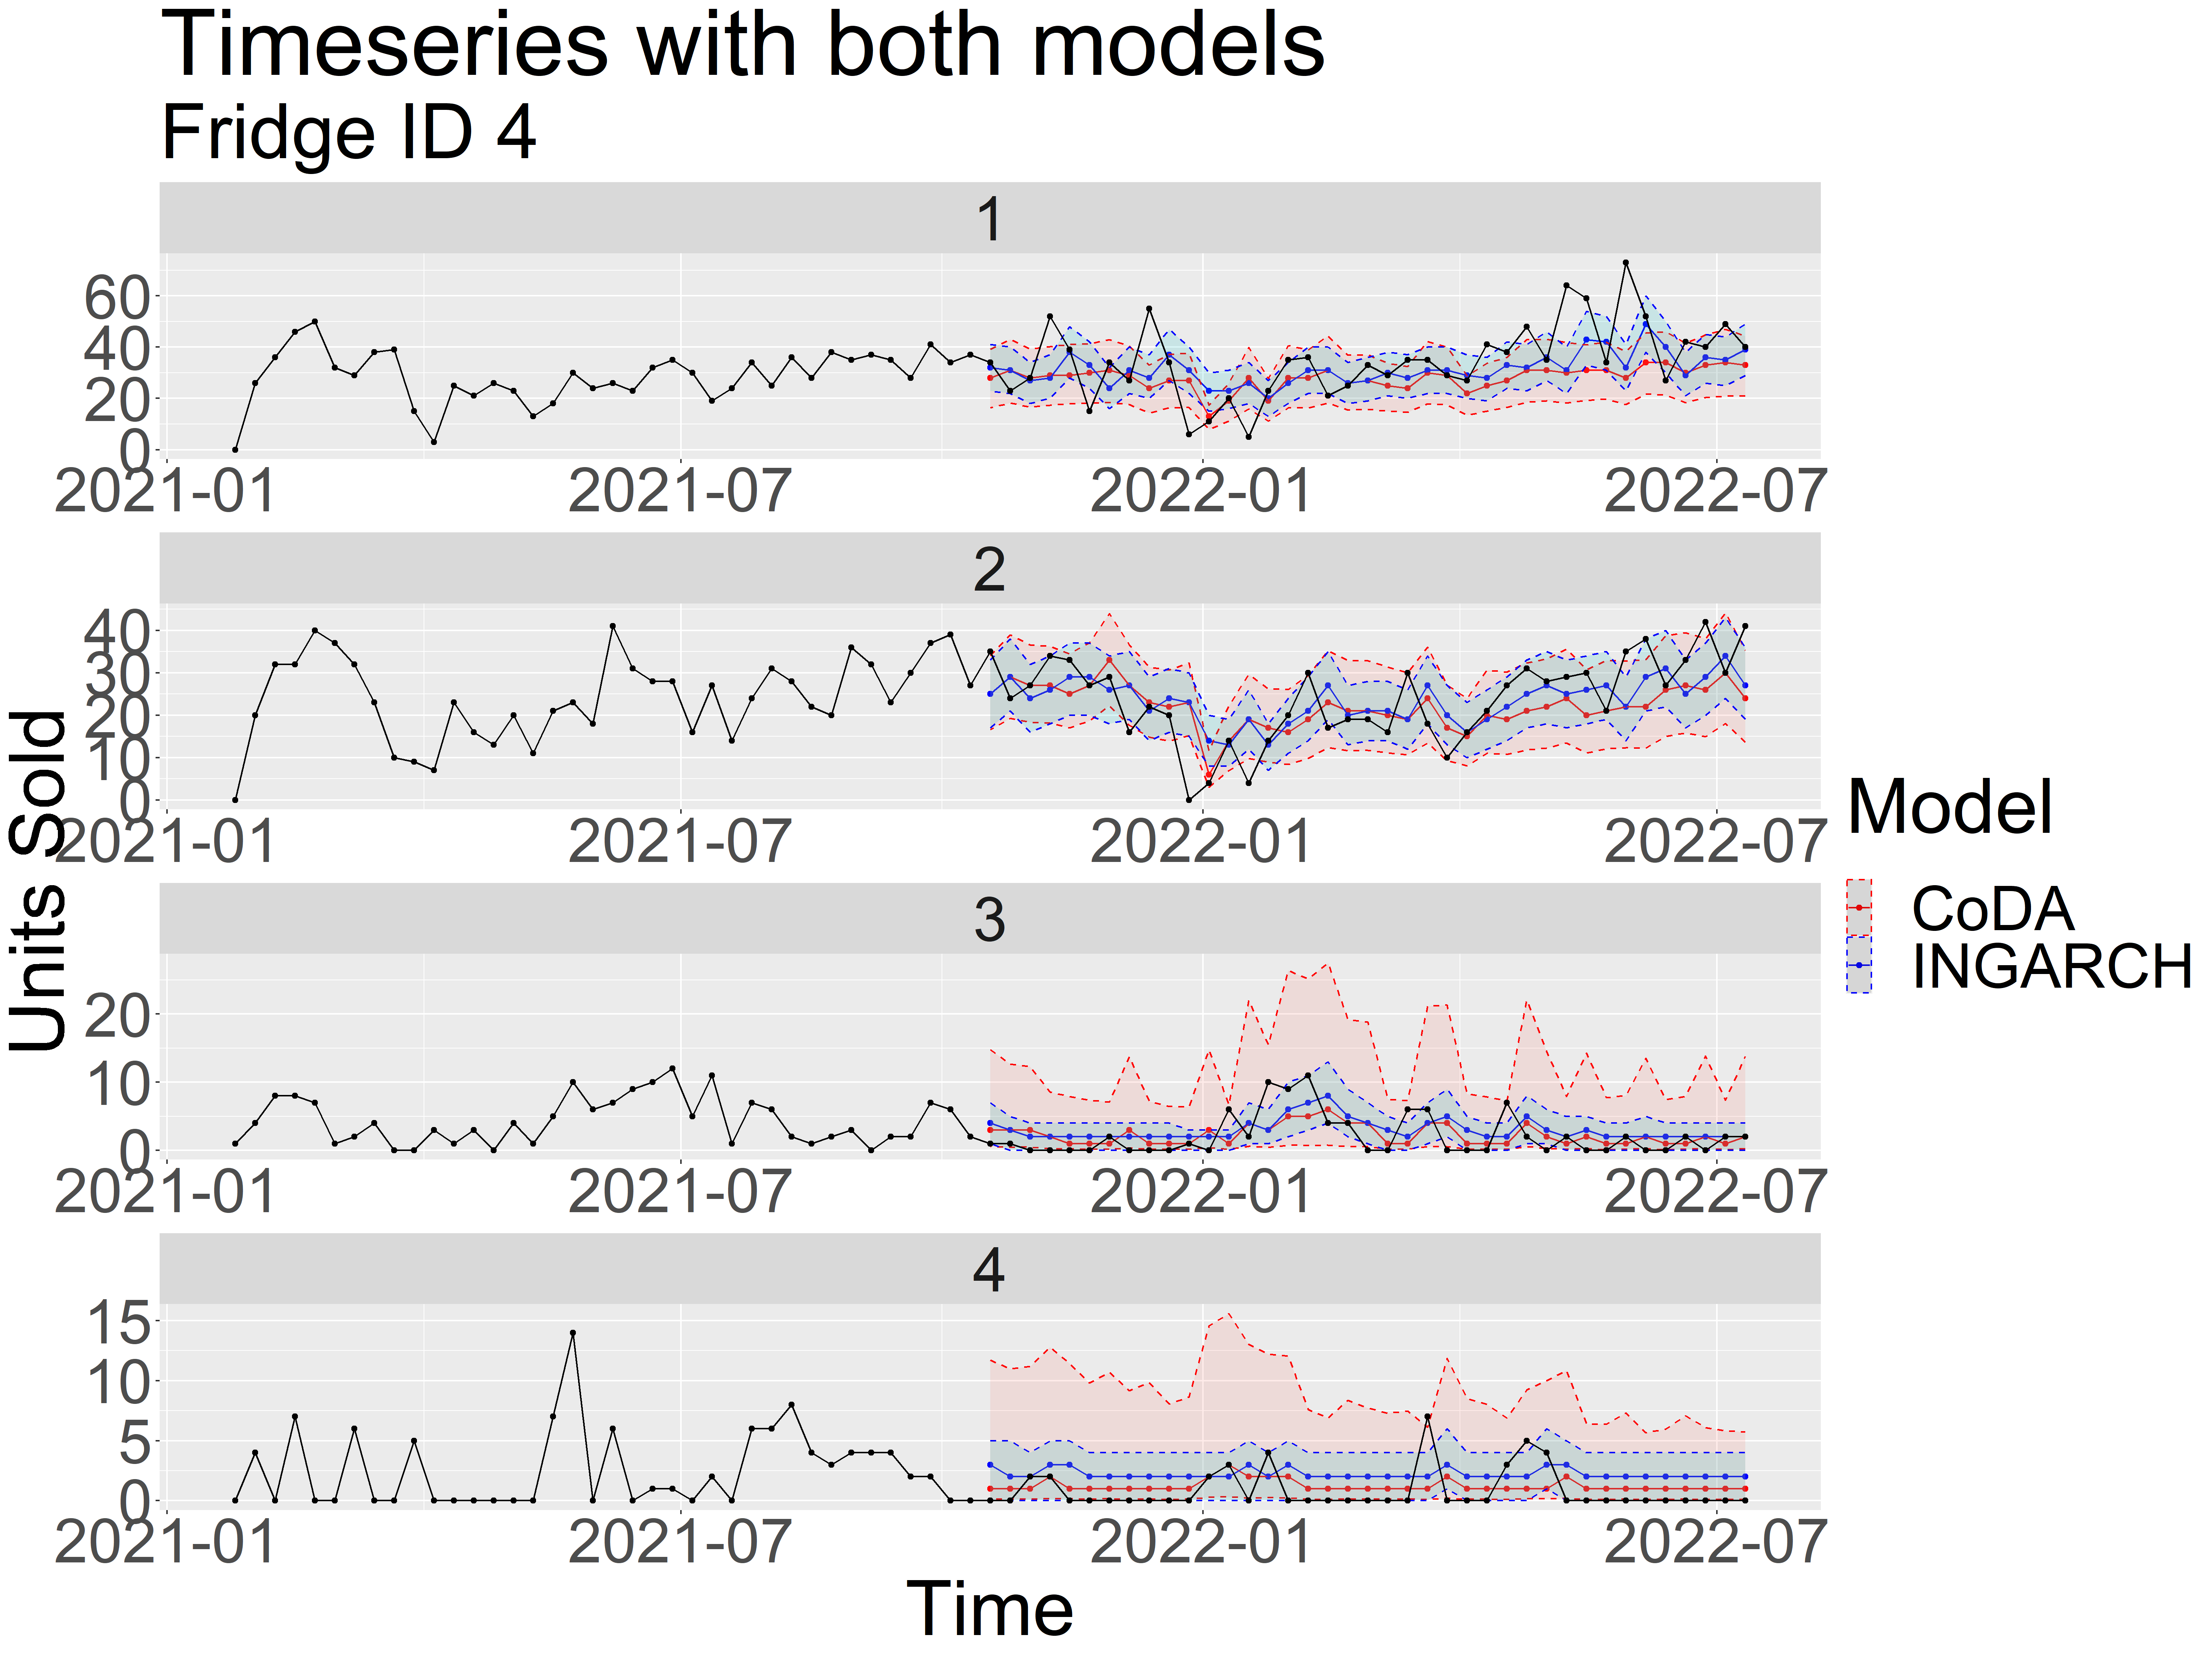
\includegraphics[width=\textwidth]{F:/Uni/Masterarbeit/Master-Thesis_git/Arbeit/Graphiken/BothPI_Timeseries_ID4.png}
\caption{Fridge 4 with the both models and their prediction intervals}
\label{fig:BothPI Fridge 4}
\end{subfigure}
\hfill
\begin{subfigure}[b]{0.8\textwidth}
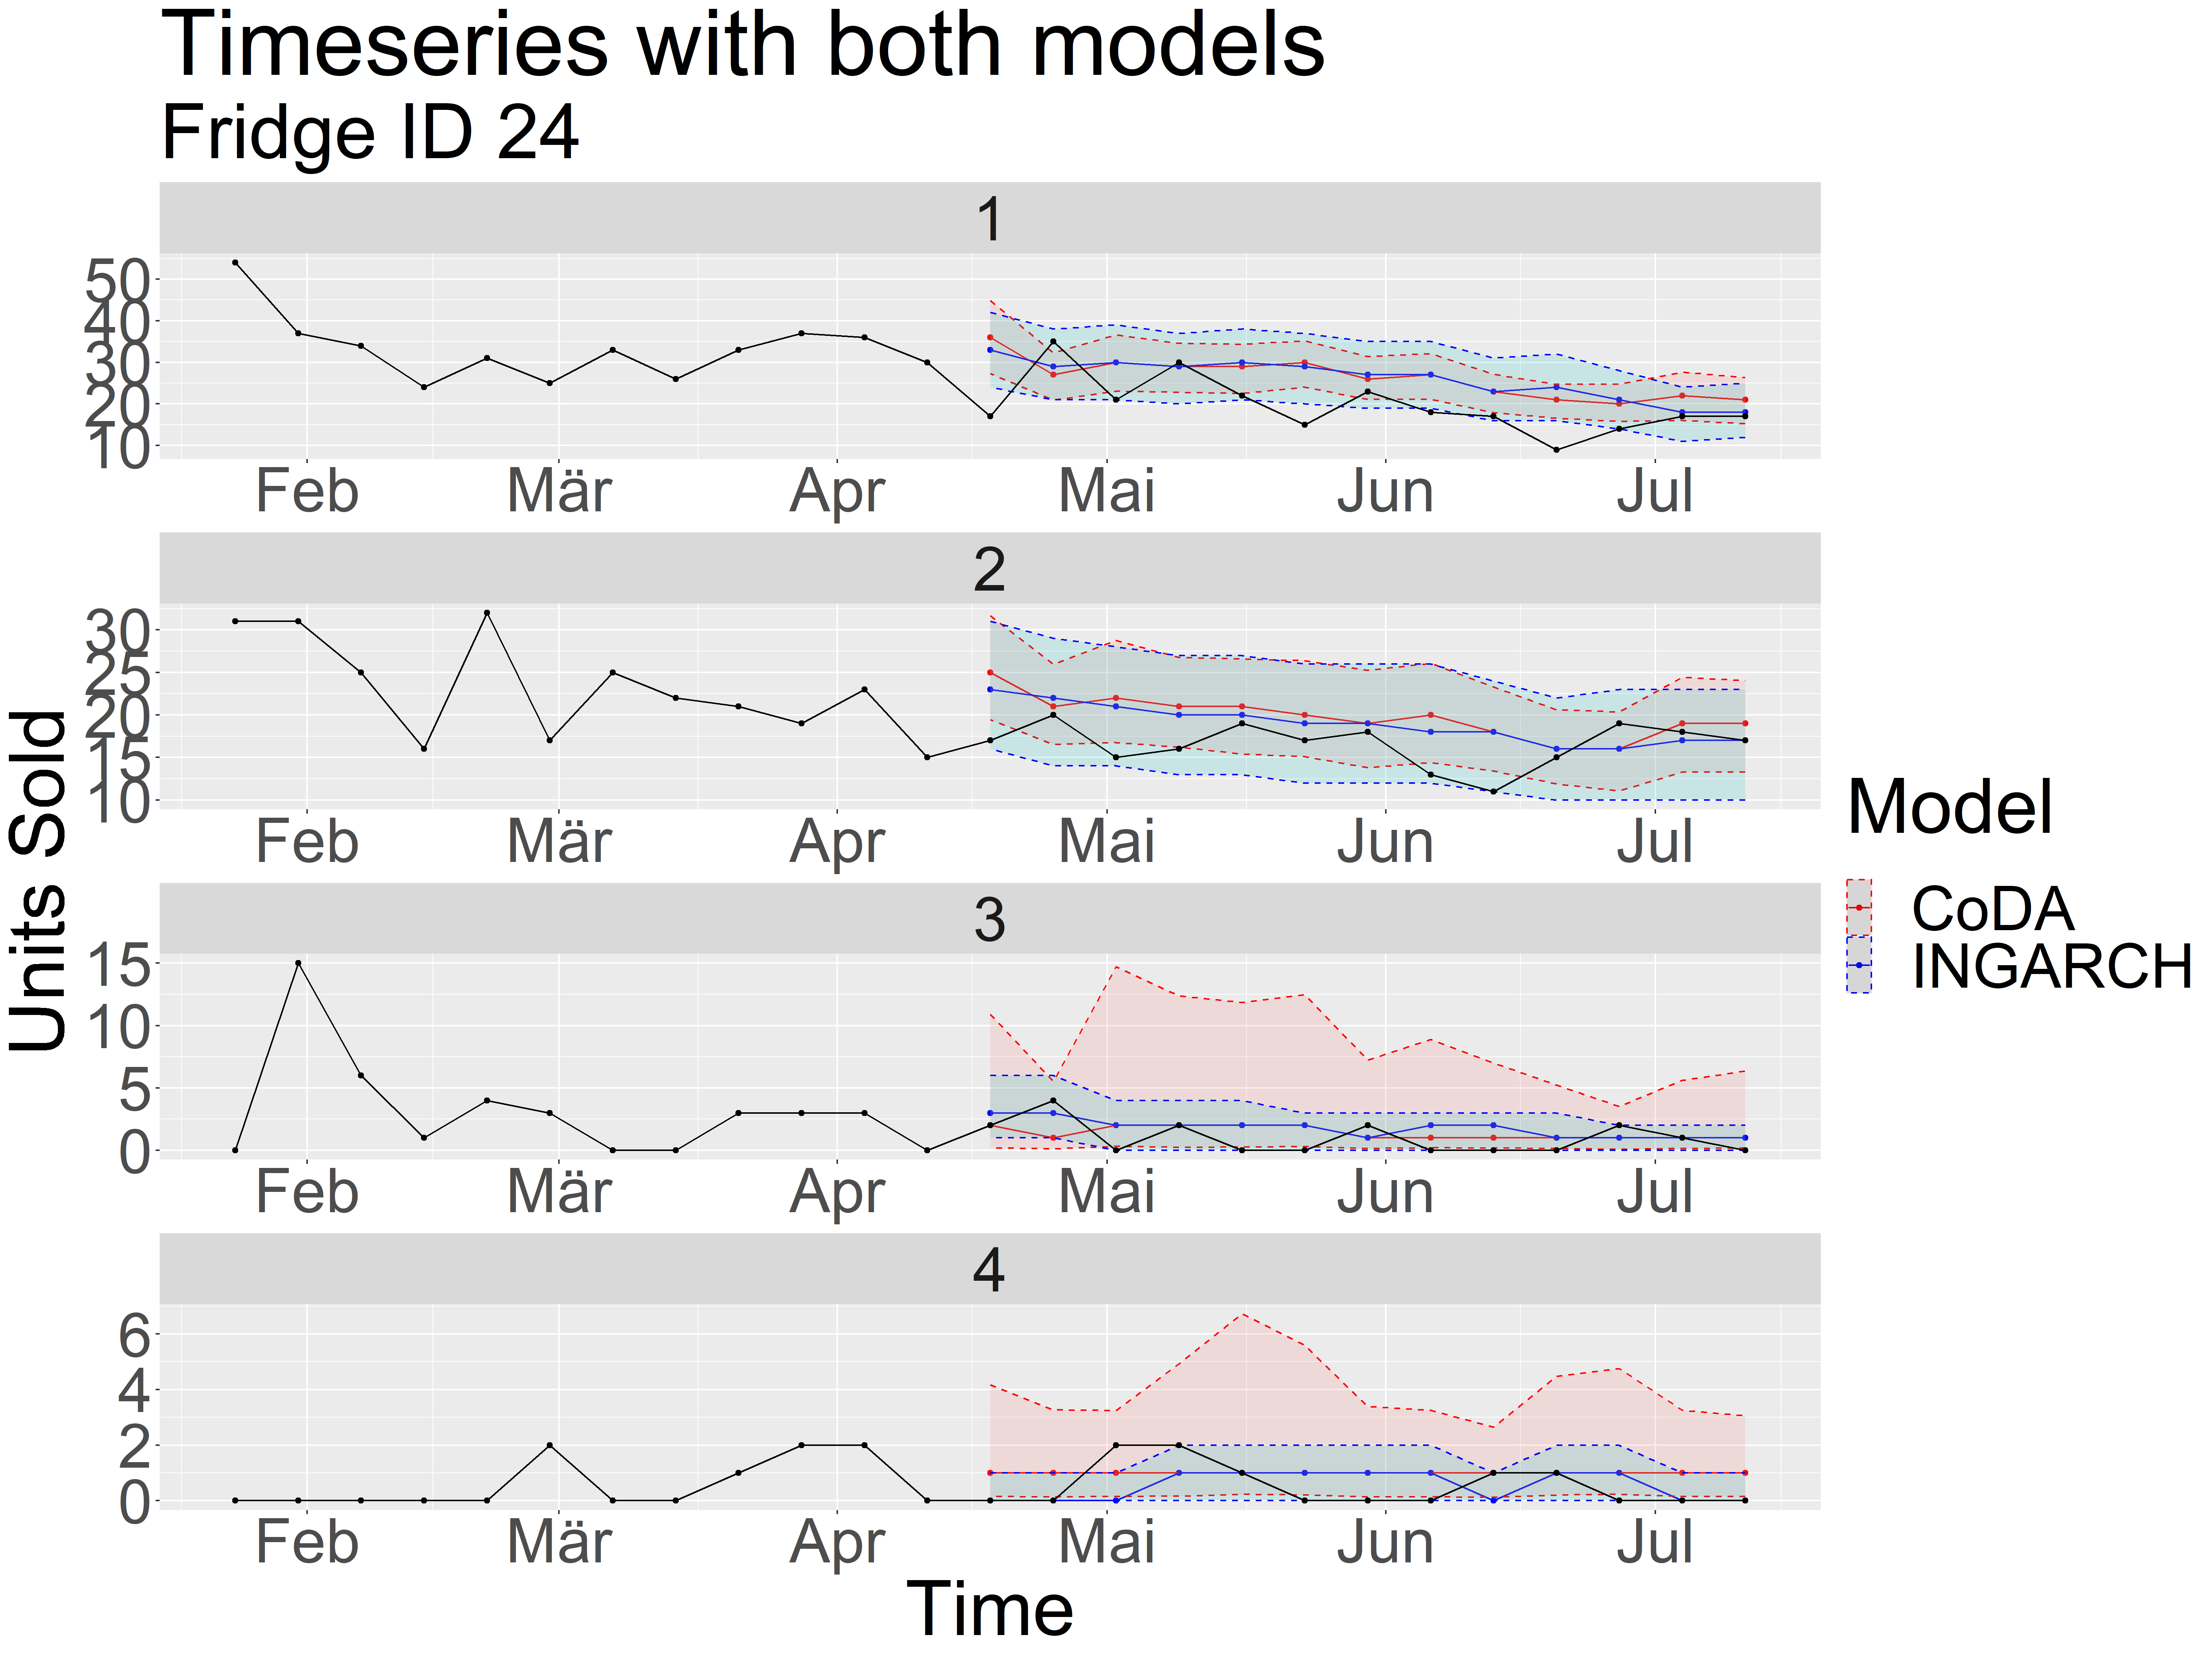
\includegraphics[width=\textwidth]{F:/Uni/Masterarbeit/Master-Thesis_git/Arbeit/Graphiken/BothPI_Timeseries_ID24.png}
\caption{Fridge 24 with the both models and their prediction intervals}
\label{fig:BothPI Fridge 24}
\end{subfigure}
\caption{Timeseries with both models and their prediction intervals}
\label{fig:TS BothPI}
\end{figure}
\section{R-Code}
\label{sec:R-Code}

\subsection{R-Packages}
\label{sec:R-Packages}

We conducted our analysis in the statistical software R, see \textcite{R:2022}. For our data cleansing, data handling and plotting we use the \textit{tidyverse} package of \textcite{Tidyverse:2019}. Further we use the packages \textit{here} of \textcite{here:2020}, \textit{miceadds} of \textcite{Miceadds:2023} and \textit{parallel}, which is part of core R, to facilitate our analysis.  

For building our CoDA model we use the packages \textit{vars} of \textcite{VAR:2008,CoDAR2:2008} and \textit{robCompositions} of \textcite{RobComp:2011,CoDAR4:2018}. Especially the functions \texttt{pivotCoord}, which performs the ilr transformation described in Section \ref{sec: Coda Preliminaries},\texttt{VAR}, which builds the VAR model described in Section \ref{sec:The VAR Model}, and \texttt{pivotCoordInv} which performs the necessary back transformation to get predictions in the desired space. The INGARCH analysis is mainly done with the package \textit{tscount}, see \textcite{Tscount:2017,Tscount:2020}. The core function used is \texttt{tsglm} which we use to fit the INGARCH(p,q) model as well as the log-linear model. The zero-inflated models were fitted using the function \texttt{zeroinfl} from the package \textit{pscl} of \textcite{Pscl:2008}. For the VGAM we used the package \textit{VGAM} of \textcite{RVGAM:2010}. To fit the INAR model we use two packages. First \textit{ZINAp} to calculate our predictions with the Bayesian approach. The function \texttt{estimate\_zinarp} is used to estimate the coefficients and the values are then calculated according to the formula in \textcite{Silva:2009}. Second, the classical approach was done using the function \texttt{EST\_ZINAR} from the package \textit{ZINA1}.

In general, all functions can be grouped into three categories: general, count data model specific and CoDA specific. General functions are used for both, the count data models and the CoDA model. Count data models and CoDA specific functions are only used for their respective methods.
\subsection{Handbook}
\label{sec:Handbook}

In this handbook, we will describe the use and results of the most important functions used for our analysis.  The code for them can be found in the GitHub repository, see \textcite{GitHub}. 

\subsubsection{Data.Window}
\label{sec: Data.Window}
%Notable general functions are \texttt{Data.Window} and \texttt{Data.Preparation}. The former function splits the time series in the specified windows and the value to be predicted. The models are then fitted on these windows and the prediction result is compared with the actual value. The latter one brings the data in the right format, replaces missing values with 0 and accounts for the length of the history chosen. In addition, for CoDA it also transform the data into the right format needed for the one-vs-all method. Other important functions are \texttt{Model.Error} and \texttt{Model.ErrorOverall} which implement the error measure introduced in \ref{sec: Error Measure} and summarise it. 

The function \texttt{Data.Window} splits the time series in the specified windows and the value to be predicted. The models are then fitted on these windows and the prediction result can be compared with the actual value.

\textbf{Arguments}:

\begin{itemize}
	\item Timeseries: The time series to be split up in windows.
	\item Frame: The window length to split the time series into.
	\item Method: How the time series should be split up. For example if the windows should be extended at each step or be kept at a fixed length.
	\item PredictionStep: The future prediction step.
\end{itemize}

\textbf{Values}:

A list of all windows is returned. A window is a list with the following elements: 

\begin{itemize}
	\item timeSeriesValue\_window: The values of the window
	\item timeSeriesValue\_future: The value which should be predicted by this window. 
\end{itemize}

\subsubsection{Data.Preparation}
\label{sec:Data.Preparation}

The function \texttt{Data.Preparation} brings the data in the right format, replaces missing values with 0 and accounts for the length of the history chosen. In addition, for CoDA it also transforms the data into the right format needed for the one-vs-all method.

\textbf{Arguments}:

\begin{itemize}
	\item Data\_Raw: The Data to be transformed in the right format.
  \item OneVsAll: When TRUE, then the one-vs-all method is used.
  \item PivotGroup: When one-vs-all is used, this specifies the pivot category.
  \item Category: The categories to consider for the transformation.
  \item NA\_to: The value with which NA values should be replaced with.
  \item HistoryLength: The length of the history. Can be an absolute number or a ratio $0<h\leq 1$. 
  \item TakeSubCategory: When TRUE, then we transform the data for the subcategories instead of the main categories. 
\end{itemize}

\textbf{Values}:

A tibble with two or more columns is returned, depending on the number of categories: 

\begin{itemize}
	\item week\_date: The values of the window
	\item \textit{Name of Category 1}: The number of sold items belonging to \textit{Name of Category 1}.
\end{itemize}

When the argument OneVsAll is TRUE, then a tibble with three columns is returned.


\begin{itemize}
	\item week\_date: The values of the window
	\item PivotGroup: The amount of sold items belonging to the pivot group.
	\item other: The amount of all other sold items belonging to the other categories. 
\end{itemize}

\subsubsection{Model.Error}
\label{sec:Model.Error}

The function \texttt{Model.Error} calculates the specified error measure for each time series and category. Since we want to compare the performance of a method with the one of the naive model in Section \ref{sec: Naive Random Walk} we calculate the errors for this model as well. 

\textbf{Arguments}:

\begin{itemize}
	\item Model\_Result: The result calculated by either \texttt{Coda.Analysis} or \texttt{CountModel.Analysis}.
	\item Fnct: The error function to be used. Currently the MSE and RMSE are implemented. 
	\item Category: The categories for which the errors should be caluculated.
\end{itemize}

\textbf{Values}:

A tibble with the columns is returned: 

\begin{itemize}
	\item id: The id of the fridge.
	\item category: The category for which the error was calculated. 
	\item error: The error calculated according to the error function in the Fnct argument. 
	\item error\_naive: The value of the error function for the naive random walk model.
	\item model: The used model.  
\end{itemize}

\subsubsection{Model.ErrorOverall}
\label{sec:Model.ErrorOverall}

The function \texttt{Model.ErrorOverall} is closely related to \texttt{Model.Error}. This function calculates the error measure defined in Section \ref{sec: Error Measure}. One can decide if the error measure should be calculated over all categories or if they should be split up in subsets as in Subsection \ref{sec:Error Measure Extension}.

\textbf{Arguments}:

\begin{itemize}
	\item Error\_Result: The result of the function \texttt{Model.Error}.
	\item Fnct: Function to summarise the errors. This enables one to use different methods like the mean or median. 
	\item SplitByGroup: When TRUE, then the errors are split by groups defined in the \textit{Groups} argument. 
	\item Groups: The grouped categories over which the error should be calculated. 
	\item Category: The categories for which the error should be calculated for.
\end{itemize}

\textbf{Values}:

The result is a tibble with the columns:
\begin{itemize}
	\item id: The id of the fridge. 
	\item error: The error calculated according to the error function in the Fnct argument. 
	\item model: The used model. 
	\item group: The subsets of categories as defined in Subsection \ref{sec:Error Measure Extension}.
\end{itemize}


\subsubsection{CountModel.DataPreparation}
\label{sec:CountModel.DataPreparation}

The function \texttt{CountModel.DataPreparation} transforms the data into the right format needed to fit the count data models. At its core it uses the \texttt{Data.Preparation} function but adds the additional option to replace zero values with 1. 

\textbf{Arguments}:

\begin{itemize}
	\item Data: The data to be transformed.
	\item ZeroHandling: Method for zero handling. Currently there is no treatment or them being replaced with 1. 
	\item HistoryLength: The length of the history. Can be an absolute number or a ratio $0<h\leq 1$. 
	\item TakeSubCategory: When TRUE, then we transform the data for the subcategories instead of the main categories. 
\end{itemize}

\textbf{Values}:

A tibble with two or more columns is returned, depending on the number of categories: 

\begin{itemize}
	\item week\_date: The values of the window
	\item \textit{Name of Category 1}: The number of sold items belonging to \textit{Name of Category 1}.
\end{itemize}

\subsubsection{CountModel.Prediction}
\label{sec:CountModel.Prediction}

The function \texttt{CountModel.Prediction} is the function where the model is fit and the predicted value is calculated. It uses the corresponding functions mentioned in Section \ref{sec:R-Packages} to fit the INGARCH,INAR or ZIM model for each window and predicts the next value. 

\textbf{Arguments}:

\begin{itemize}
	\item Data\_Window: The data divided into the different windows by the \texttt{Data.Window} function.
	\item Data\_WindowNoTransform: The data without zero handling divided into the different windows by the \texttt{Data.Window} function.
  \item Category: The category to predict. 
  \item PredictionStep: The prediction step.
  \item Frame: The window length.
  \item Distribution: The distribution chosen for the model. Care has to be taken, since every model can choose from a different list of distributions and its name has to be specified correctly (i.e. "`Po"' for INAR but "`poisson"' for ZIM). 
  \item Plot: For the INGARCH model, diagnostic plots can be generated. Currently not implemented.
  \item WindowMethod: Method for splitting up the time series. For example if the windows are extended at each step or kept at a fixed length.
  \item External: For INGARCH. When TRUE, external factors as in Equation (\ref{eq:Ingarch model with external effect}) are used.
  \item PastOb: For INGARCH. How many past observations should be used. Equals $p$ in Equation (\ref{eq:Ingarch model}).
  \item PastMean: For INGARCH. How many past means should be used. Equals $q$ in Equation (\ref{eq:Ingarch model}).
  \item ModelType: Model to be fit. 
\end{itemize}

\textbf{Values}:

It returns a list with two elements:

\begin{itemize}
	\item prediction: A data.frame with the predicted values and some additional information.
	\item model: A list of all the models fitted for each window. 
\end{itemize}


\subsubsection{CountModel.Analysis}
\label{sec:CountModel.Analysis}


The function \texttt{CountModel.Analysis} acts as a wrapper function to streamline and facilitate the analysis. The previously mentioned model specifications can be chosen here as well as various other options. This is the sole function which has to be used by the user. The other functions are mainly for internal use.

\textbf{Arguments}:

\begin{itemize}
	\item Data\_Raw: The raw data as extracted from the data base.
  \item Id: The ids of the fridges to be analysed.
  \item PredictionStep: The future prediction step.
  \item Distribution: The distribution chosen for the model. Care has to be taken, since every model can choose from a different list of distributions and its name has to be specified correctly (i.e. "`Po"' for INAR but "`poisson"' for ZIM).
  \item ModelType: Model to be fit. 
  \item Plot: For the INGARCH model, diagnostic plots can be generated. Currently not implemented.
  \item Category\_Main: The main categories to choose. 
  \item TakeSubCategory: When TRUE, then we transform the data for the subcategories instead of the main categories. 
  \item Category\_Sub: The sub categories to choose.
  \item Frame: The window length.
  \item WindowMethod: Method for splitting up the time series. For example if the windows are be extended at each step or kept at a fixed length.
  \item ZeroHandling: Method for zero handling. Currently there is no treatment or them being replaced with 1. 
  \item PastOb: For INGARCH. How many past observations should be used. Equals $p$ in Equation (\ref{eq:Ingarch model}).
  \item PastMean: For INGARCH. How many past means should be used. Equals $q$ in Equation (\ref{eq:Ingarch model}).
  \item External: For INGARCH. When TRUE, external factors as in Equation (\ref{eq:Ingarch model with external effect}) are used.
  \item HistoryLength: The length of the history. Can be an absolute number or a ratio $0<h\leq 1$.
  \item Multicore: When TRUE, then calculations are done on multiple cores to improve performance. Internally the parallelisation takes place across the different categories to be calculated. 
  \item NCores: The number of cores to be used for parallelisation. 
\end{itemize}

\textbf{Values}:

This function returns a list with two values:

\begin{itemize}
	\item result: The analysis result in the form of a data.frame. 
	\item model: A nested list with all models, fitted for each id, category and window.
\end{itemize}

\subsubsection{Coda.DataPreparation}
\label{sec:Coda.DataPreparation}

The function \texttt{Coda.DataPreparation} is analog to CountModel.Preparation

\textbf{Arguments}:
\begin{itemize}
  \item Data: The data to be transformed.
  \item ZeroHandling: Method for zero handling.  Currently there is no treatment, the simple replacement strategy or adding 0.5 to all values. 
  \item TSpace: When TRUE, then $\Tsp$-Spaces are used.
  \item Log: When TRUE, then the logarithm of the total sum is used in the $\Tsp$-Space.
  \item OneVsAll: When TRUE, then the one-vs-all method is used.
  \item PivotGroup: When one-vs-all is used, this specifies the pivot category.
  \item HistoryLength: The length of the history. Can be an absolute number or a ratio $0<h\leq 1$.
	\item DL: The value $\delta$ for the simple replacement strategy in (\ref{eq:simple replacement strategy}). 
\end{itemize}

\textbf{Values}:

The result is a tibble. The columns are the ilr transformed data and hence the number of columns depends on the dimension of the data:

\begin{itemize}
	\item week\_date: The values of the window.
	\item \textit{Name of ilr transformed category 1}: The ilr transformed values.
\end{itemize}

If $\Tsp$-Spaces are used then an additional column with the sum or log-sum is added:

\begin{itemize}
	\item week\_date: The values of the window.
	\item \textit{Name of ilr transformed category 1}: The ilr transformed values.
	\item tsum: Either the total sum or log-sum. 
\end{itemize}

\subsubsection{Coda.Prediction}
\label{sec:Coda.Prediction}

The function \texttt{Coda.Prediction} acts like its respective count model counterpart.

\textbf{Arguments}:

\begin{itemize}
	\item Data\_Window: The data divided into the different windows by the \texttt{Data.Window} function.
	\item Data\_WindowNoTransform: The data without zero handling and no transformation divided into the different windows by the \texttt{Data.Window} function.
	\item Data\_NoTransform: The data without zero handling and no transformation.
	\item PredictionStep: The future prediction step.
	\item OneVsAll: When TRUE, then the one-vs-all method is used.
	\item TSpace: When TRUE, then $\Tsp$-Spaces are used.
	\item Log: When TRUE, then the logarithm of the total sum is used in the $\Tsp$-Space.
	\item PivotGroup: When one-vs-all is used, this specifies the pivot category.
	\item Frame: The window length.
\end{itemize}

\textbf{Values}:

It returns a list with two elements:

\begin{itemize}
	\item prediction: A data.frame with the predicted values and some additional information.
	\item model: A list of all the models fitted for each window. 
\end{itemize}

\subsubsection{Coda.Analysis}
\label{sec:Coda.Analysis}

Again \texttt{Coda.Analysis} is the wrapper function. This is again the only function which needs to be used by the user to fit models for the specified time series.

\textbf{Arguments}:

\begin{itemize}
	\item Data\_Raw: The raw data as extracted from the data base.
	\item Id: The ids of the fridges to be analysed.
	\item Frame: The window length.
	\item ZeroHandling: Method for zero handling. 
	\item PredictionStep: The future prediction step. 
	\item Log: When TRUE, then the logarithm of the total sum is used in the $\Tsp$-Space.
	\item TSpace: When TRUE, then $\Tsp$-Spaces are used. 
	\item OneVsAll: When TRUE, then the one-vs-all method is used. 
	\item PivotGroup: When one-vs-all is used, this specifies the pivot category.
	\item HistoryLength: The length of the history. Can be an absolute number or a ratio $0<h\leq 1$. 
	\item ModelType: Model to be fit. Currently only ``coda'' and ``coda\_OneVsAll'' can be chosen.
	\item WindowMethod: Method for splitting up the time series. For example if the windows are be extended at each step or kept at a fixed length.
	\item DL: The value $\delta$ for the simple replacement strategy in (\ref{eq:simple replacement strategy}). 
\end{itemize}

\textbf{Values}:

This function returns a list with two values:

\begin{itemize}
	\item result: The analysis result in the form of a data.frame. 
	\item model: A nested list with all models, fitted for each id, category and window.
\end{itemize}



\section{Results}
\label{sec:Results}

In this section we present and describe the results for our methods with their variations. For this we use the previously introduced error measure, calculate it for all available fridges and summarise the results. We show the results as graphics for easier interpretation. Since we focus on the CoDA and INGARCH models, we only present the in detail results for them. For a general comparison, the ZIM and INAR model are included as well. 

\subsection{Model Comparison}
\label{sec: Model Comparison}

Here we compare the INGARCH(1,1) model with the CoDA and INAR(1) model. For all three models we use the same parameter values, namely a window factor of $w=0.5$, the whole history $h=1$ and extending windows. For CoDA, the settings are no $\Tsp$-Space, one-vs-all method and the simple replacement strategy with $\delta=0.1$. For INGARCH(p,q) we use $p=q=1$, assume it is Poisson distributed, use no external factors and have no zero handling. For INAR(1) we use the classical forecasting method described in \ref{sec: Inar Parameter Estimation and Forecasting}. When we speak of standard settings or values in the following, we mean these settings. 

In \ref{fig:models Comp1} we see a boxplot and quantile plot. In the boxplot the error measure is calculated for all groups and all fridges for each model. The result is then shown in a boxplot. In the quantile plot, the error measure for each fridge, each model and each category is calculated and sorted according to their size. The dot size indicates the length of the respective time series and the vertical lines are the 0\%,25\%,50\%,75\% and 100\% quantile.

In the boxplot \ref{fig:box distributions models} we can see that their performance is pretty similar. They all seem to outperform the the naive random walk model, which is especially true for the count data models. 
In the quantile plot \ref{fig: quantile distributions models} we see the error measure split up by category. While for category 1 and 2 all models perform reasonable well and similar, differences emerge for category 3 and 4. CoDA seems to be the clear favourite in category 4, followed by INGARCH and then INAR. However, for all models there are again time series with errors that are either too high to be shown, or that couldn't get calculated at all. 
\begin{figure}[htb!]
\centering
\begin{subfigure}[b]{0.8\textwidth}
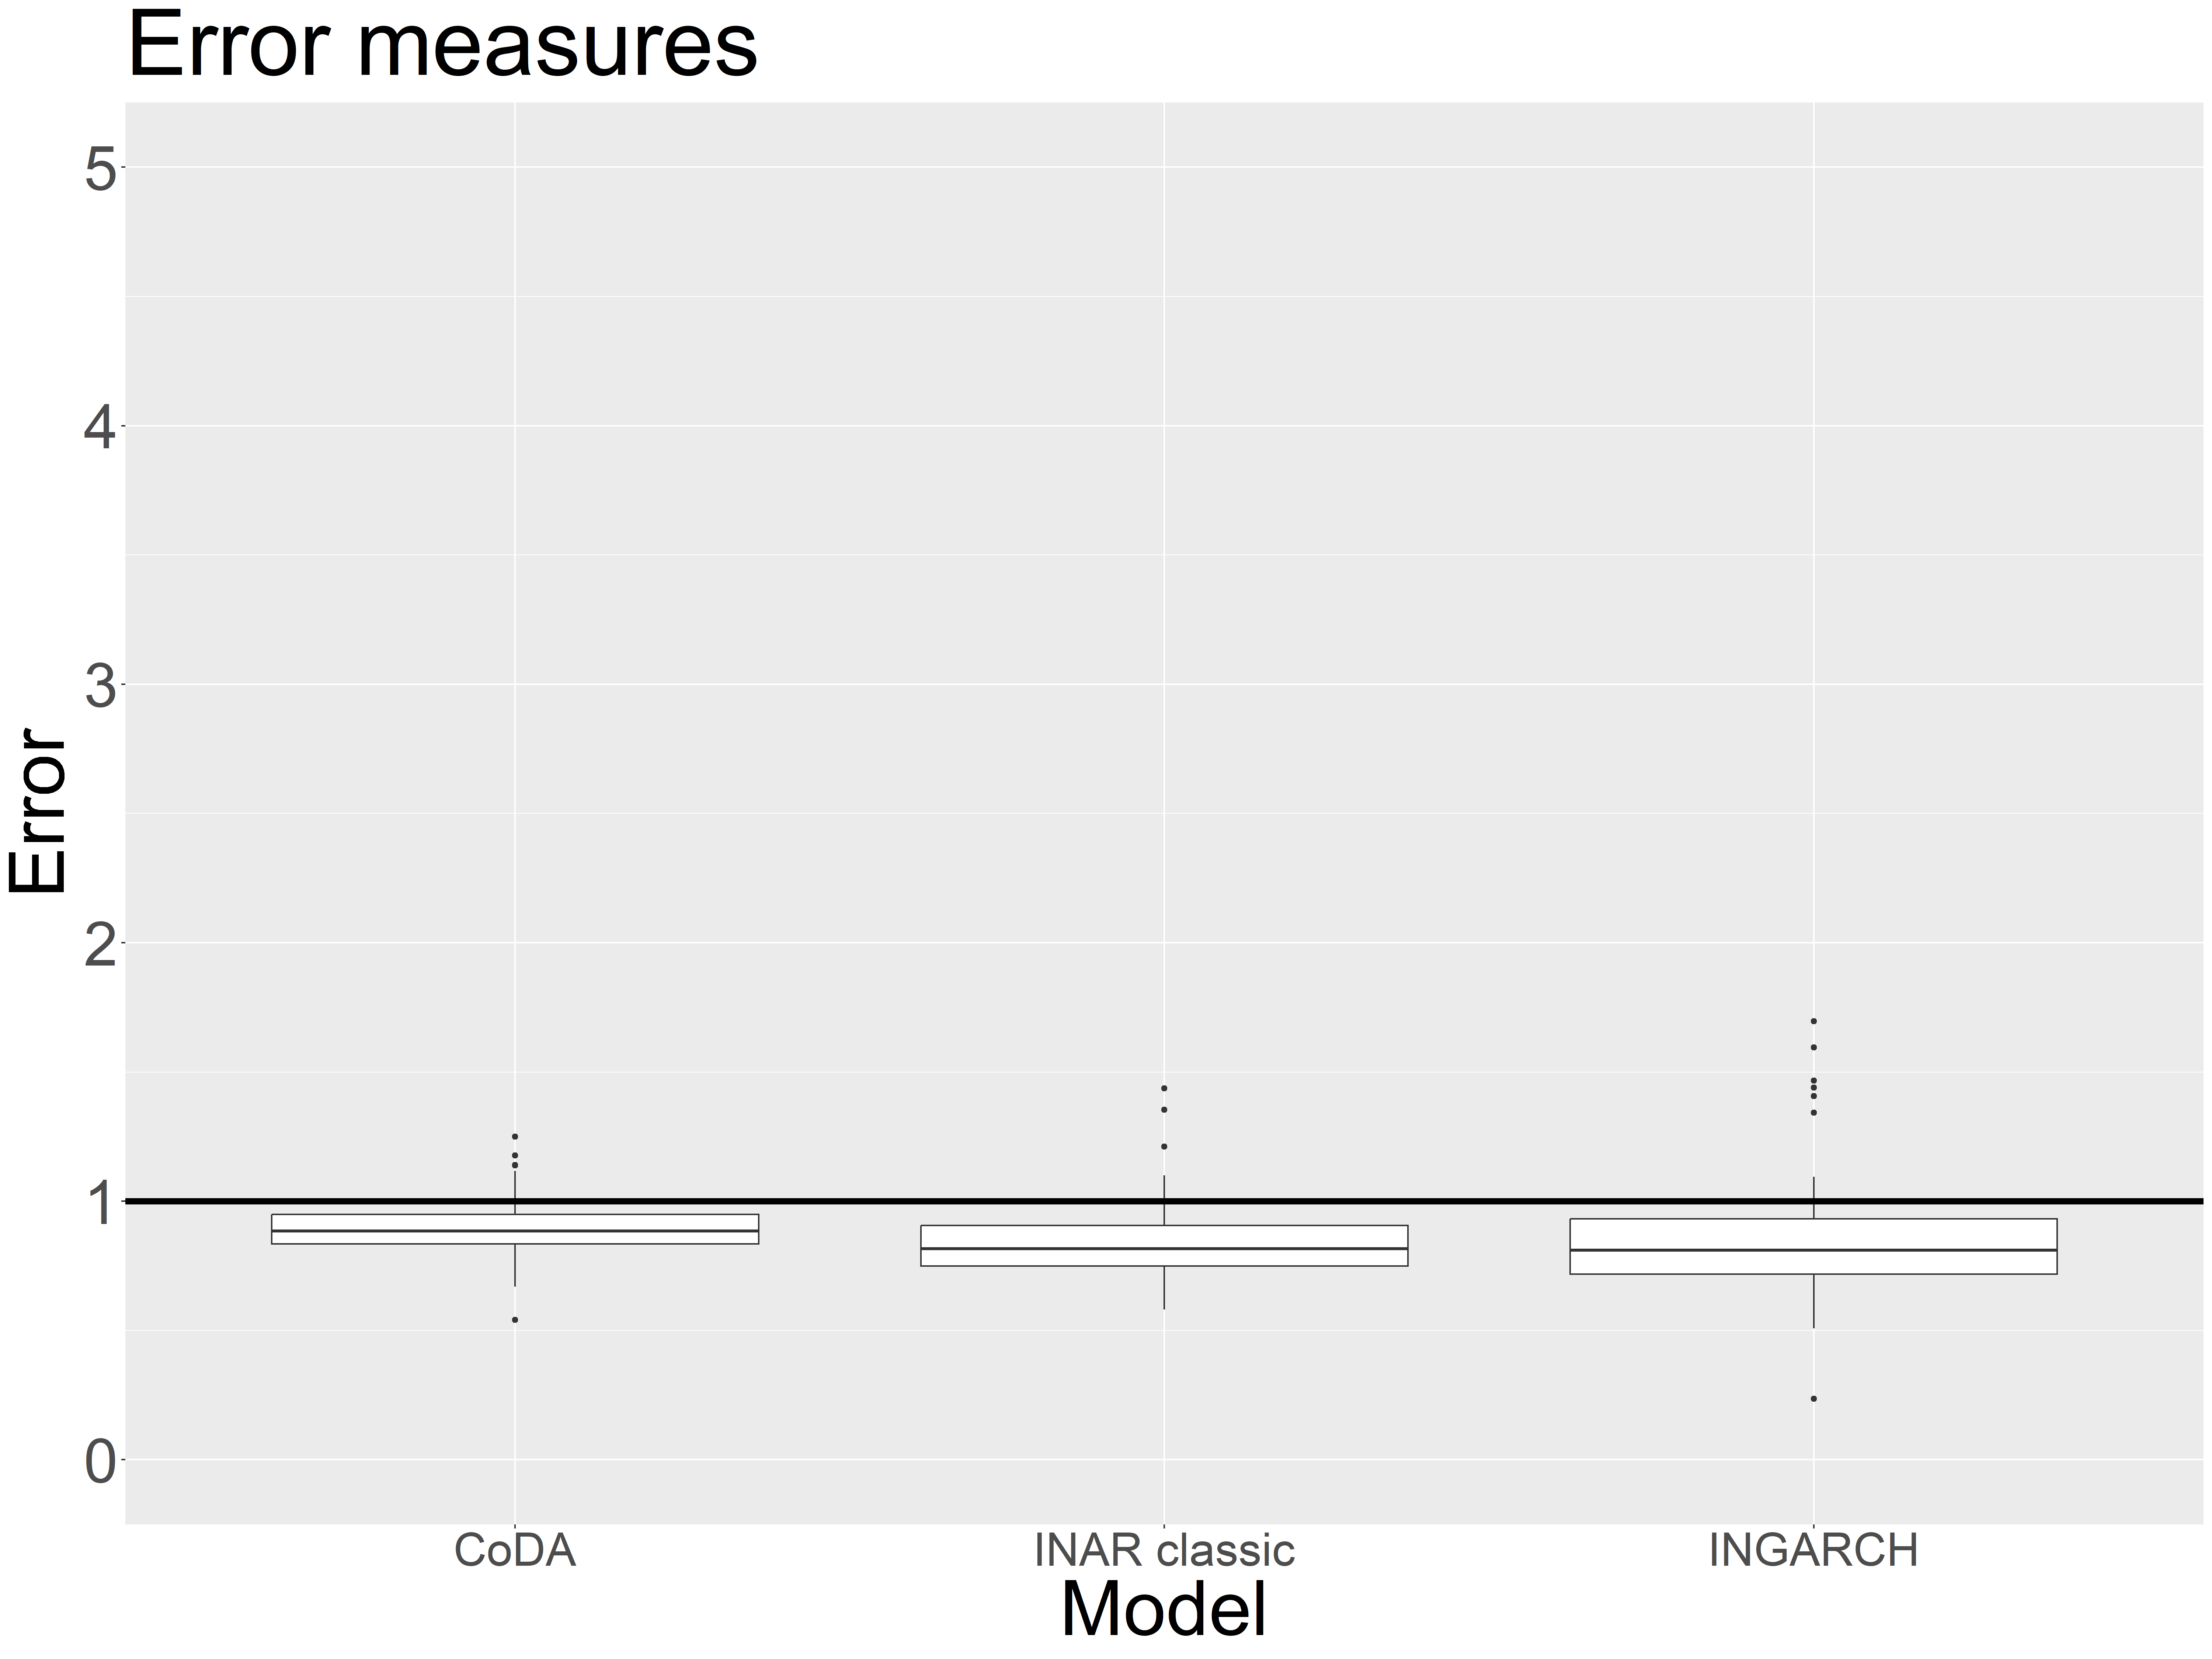
\includegraphics[width=\textwidth]{All_ErrorMeasure_combined_zoomed_ZIMFALSE.png}
\caption{Boxplot for the different models}
\label{fig:box distributions models}
\end{subfigure}
\hfill
\begin{subfigure}[b]{0.8\textwidth}
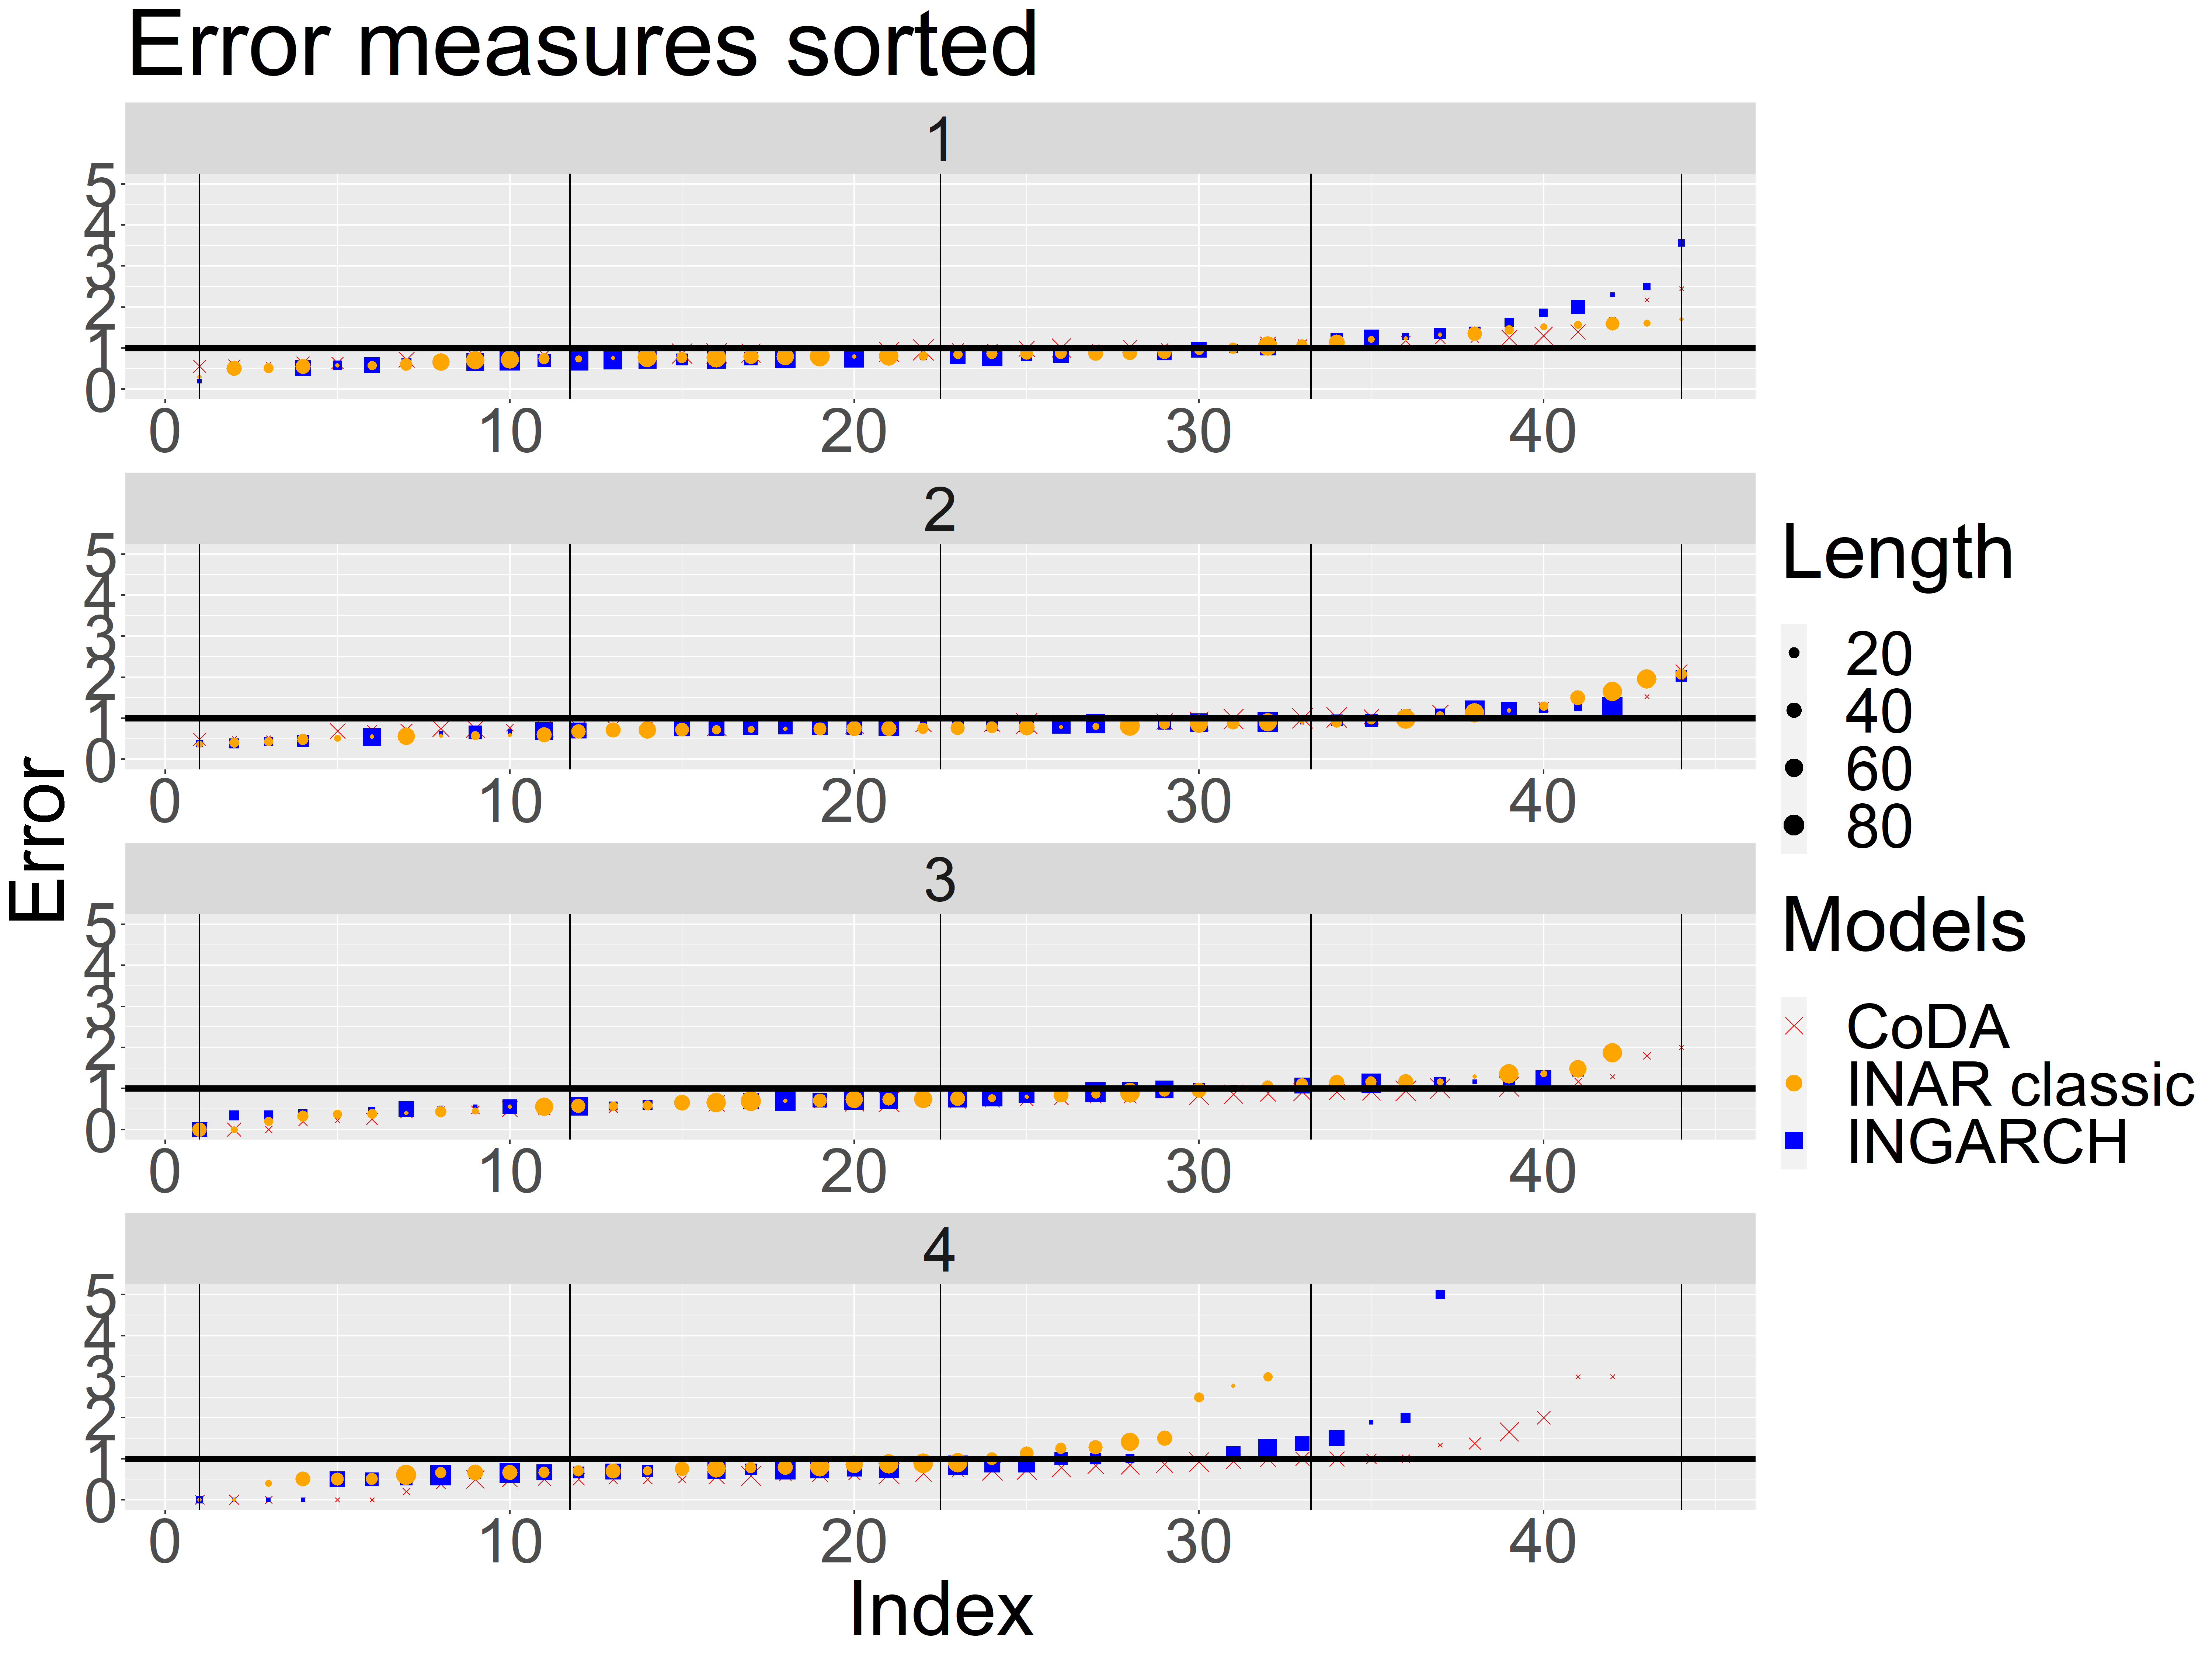
\includegraphics[width=\textwidth]{Quantile_Plot_Split_all_models_ZIMFALSE.png}
\caption{Quantiles for the different models}
\label{fig: quantile distributions models}
\end{subfigure}
\hfill
\caption{Comparison of the different models}
\label{fig:models Comp1}
\end{figure}

In figure \ref{fig:models Comp2} we also include the ZIM model. One drawback about the ZIM model is, that it needs to have zero values in the fitted window. Because of the lack of them in category 1 and 2, we couldn't manage to fit it. Hence the models in \ref{fig:models Comp2} were only fitted on categories 3 and 4. 

In \ref{fig:box distributions models Zim} we again see the boxplot for the summarised error. The ZIM is close to INGARCH, but all three models still lag behind CoDA. In \ref{fig: quantile distributions models Zim} we see again the error measure for each category. While the models perform similar for category 3, the CoDA still outperforms all models for category 4. Here it is worth mentioning, that category 4 is the main category with the most amount of zeros in our data. 

\begin{figure}[htb!]
\centering
\begin{subfigure}[b]{0.8\textwidth}
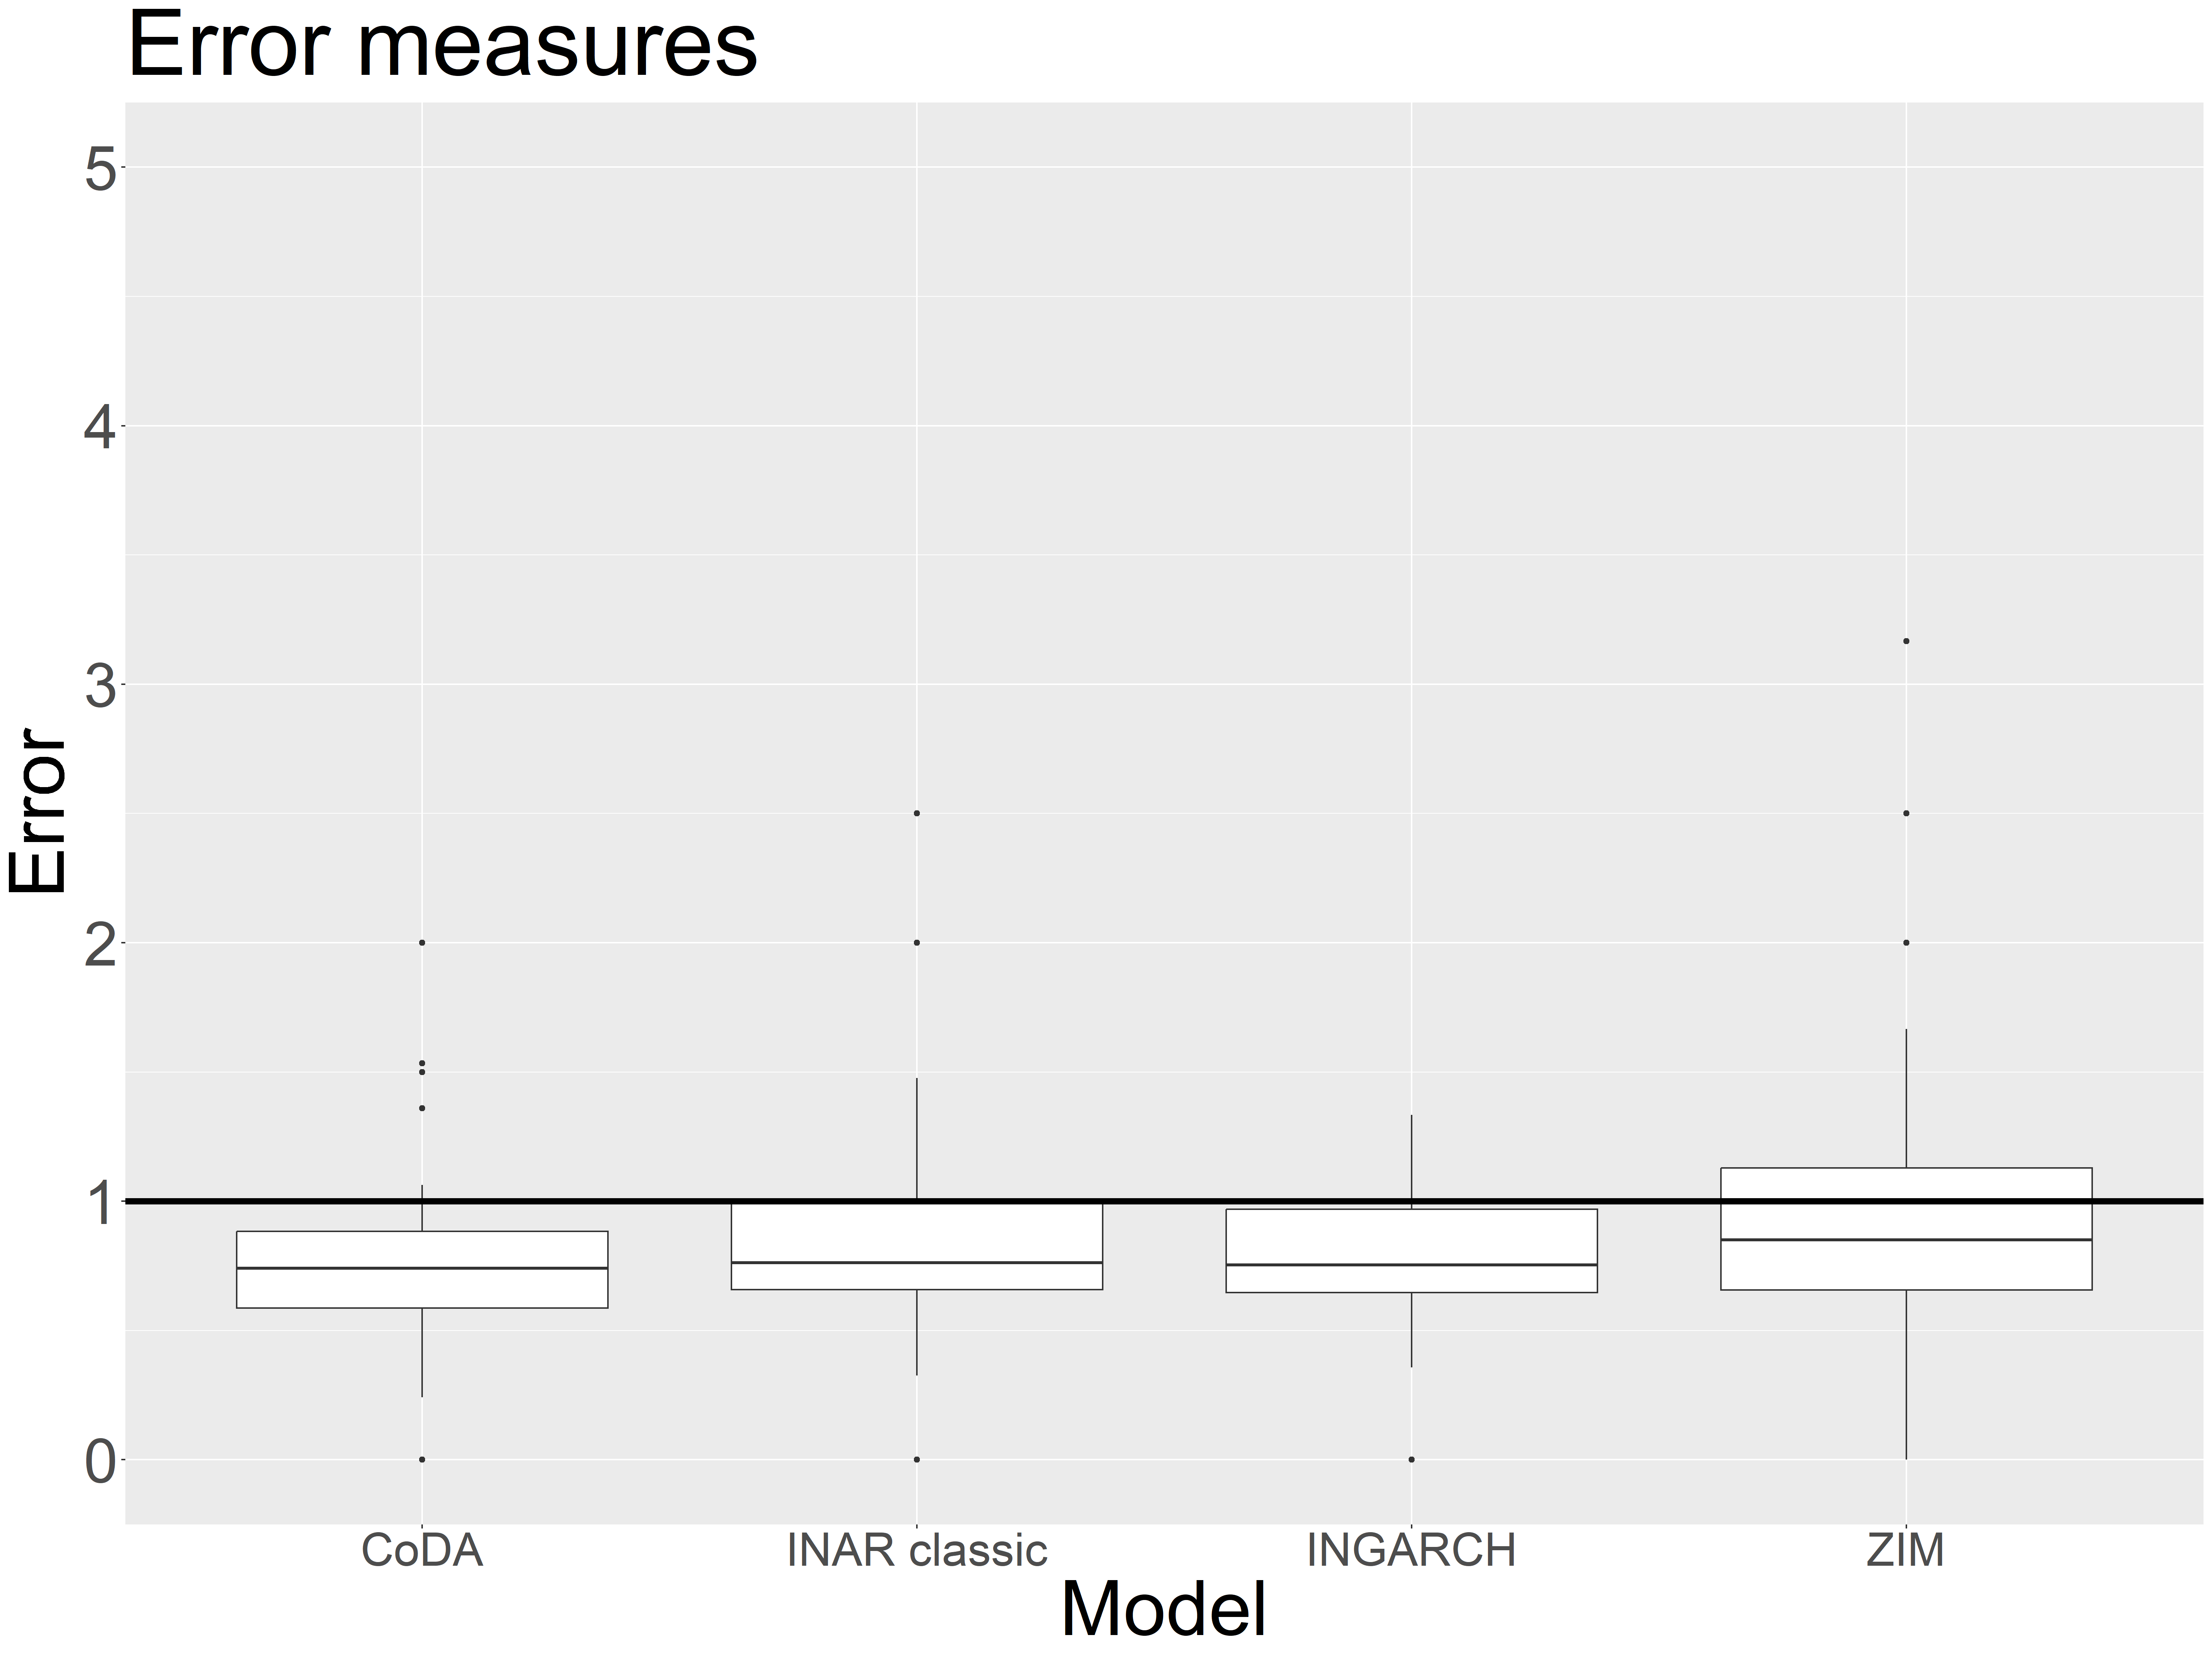
\includegraphics[width=\textwidth]{All_ErrorMeasure_combined_zoomed_ZIMTRUE.png}
\caption{Boxplot for the different models}
\label{fig:box distributions models Zim}
\end{subfigure}
\hfill
\begin{subfigure}[b]{0.8\textwidth}
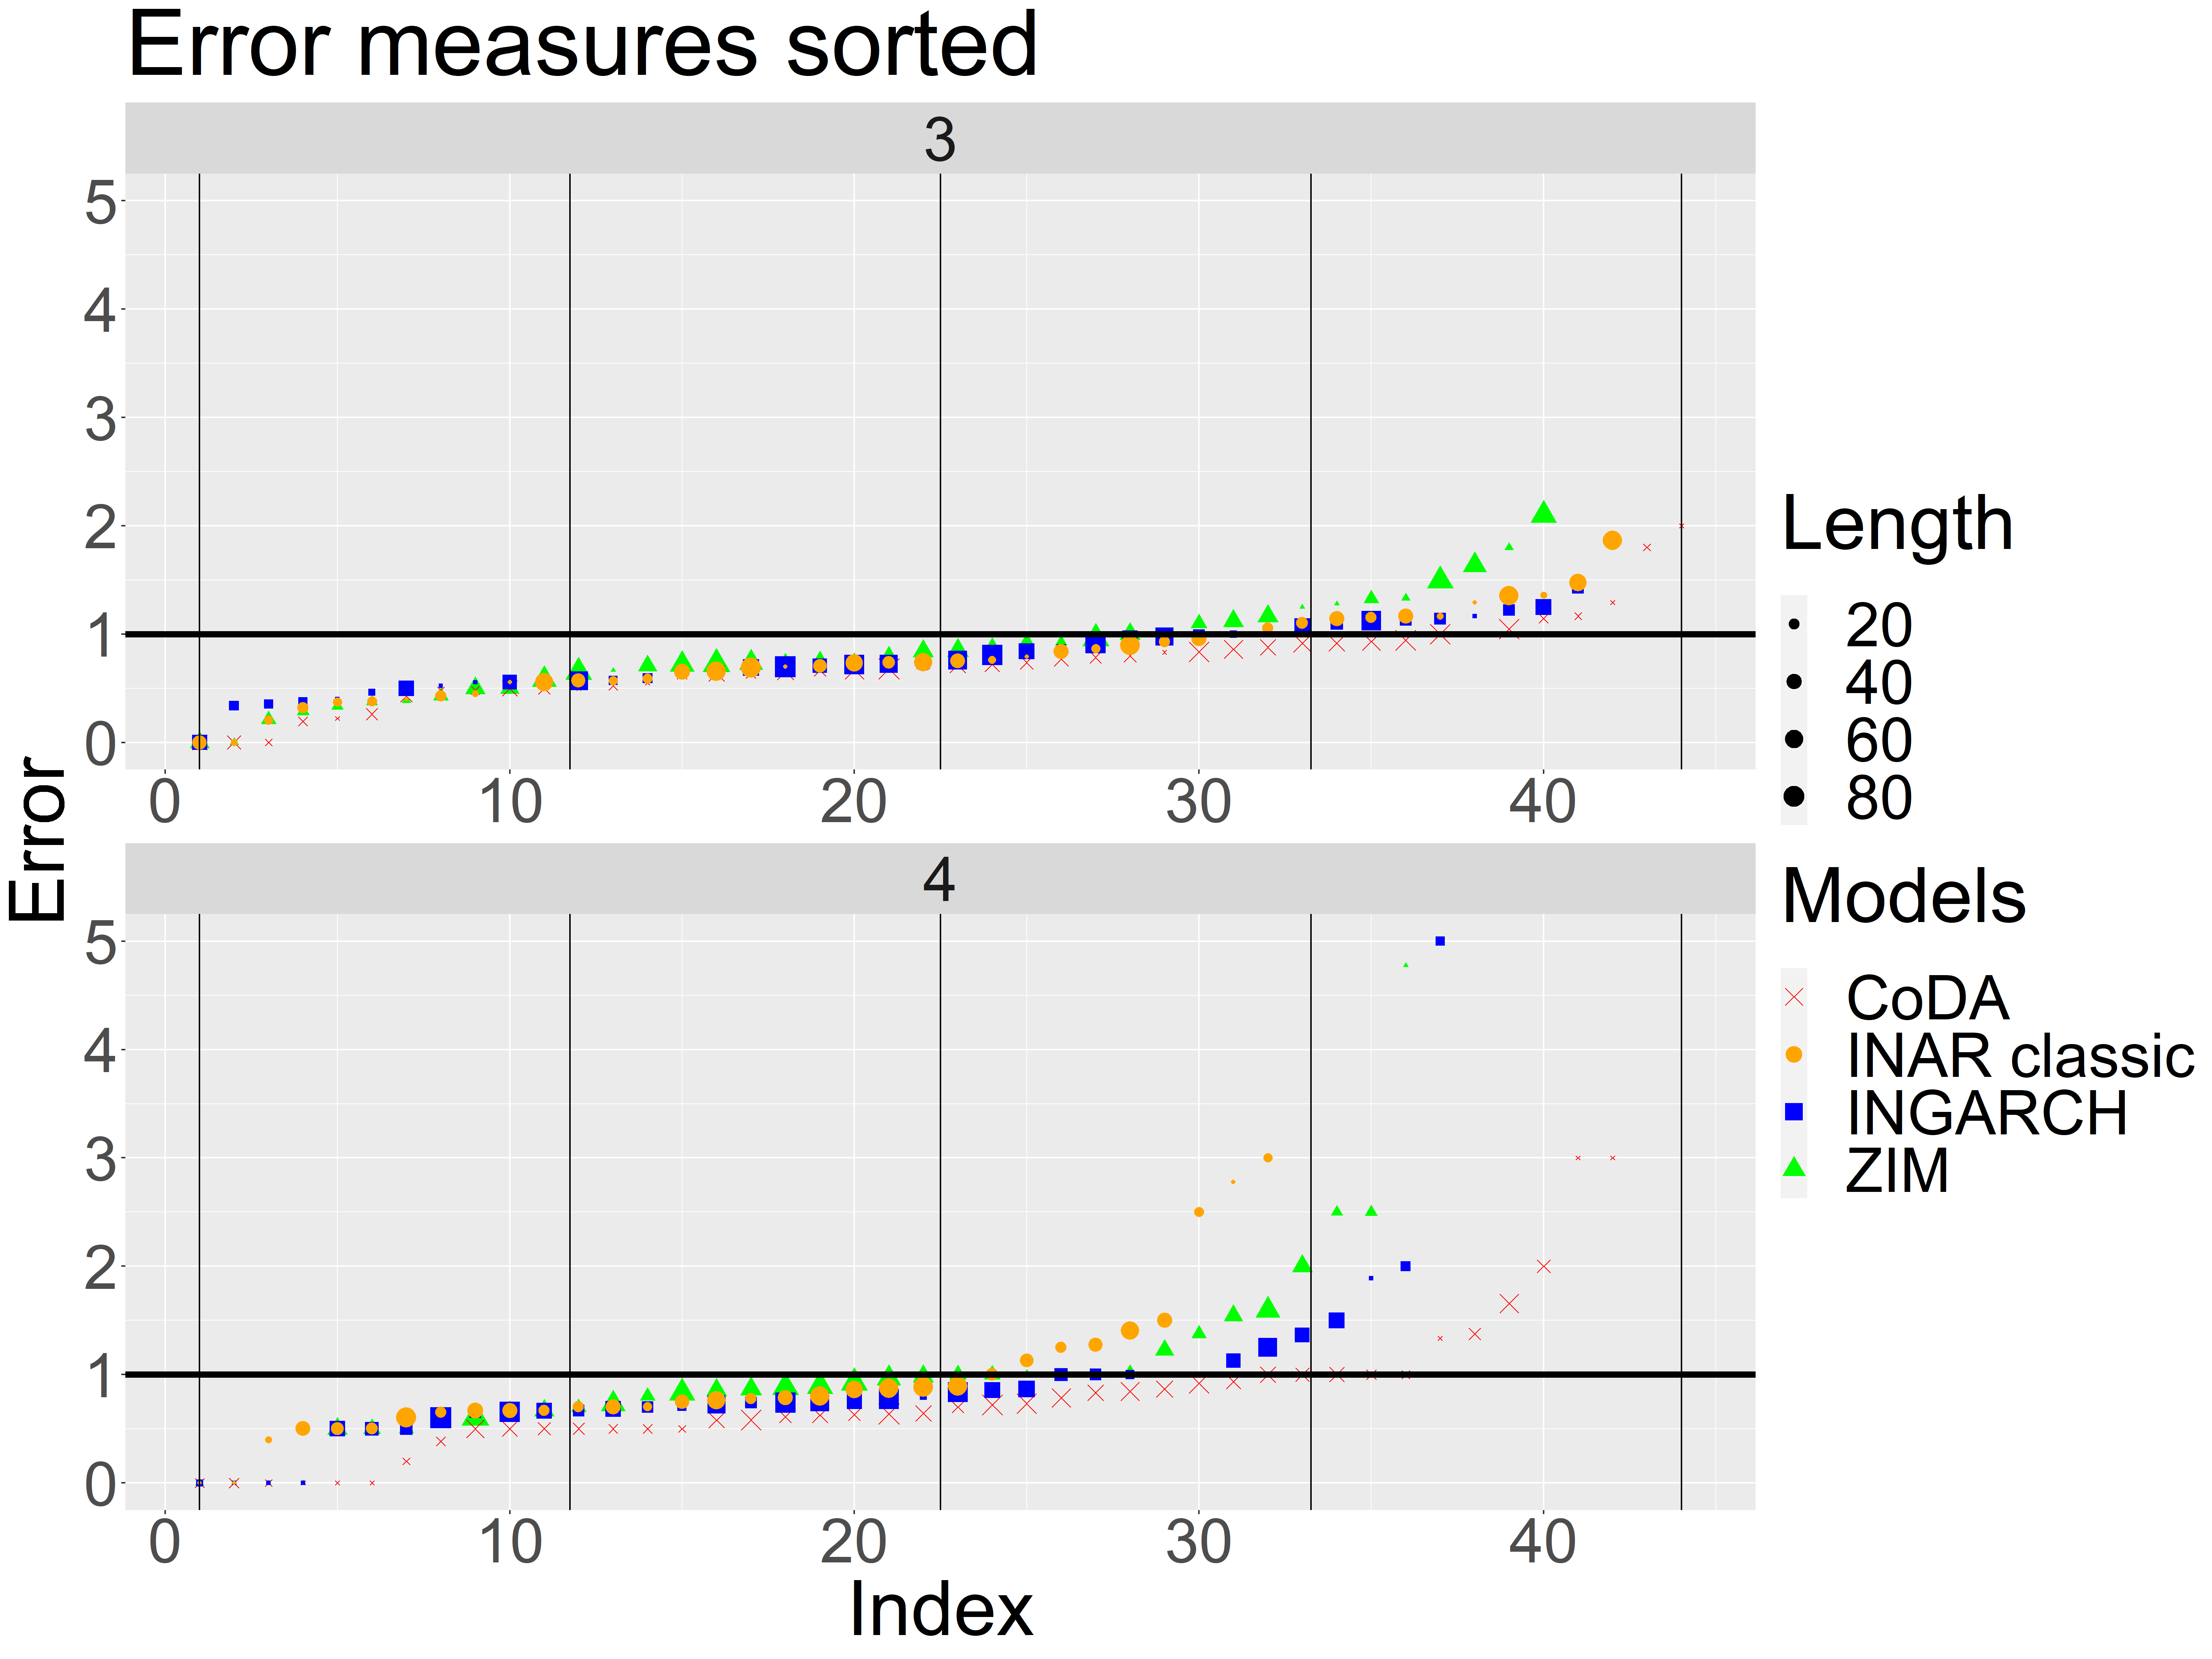
\includegraphics[width=\textwidth]{Quantile_Plot_Split_all_models_ZIMTRUE.png}
\caption{Quantiles for the different models}
\label{fig: quantile distributions models Zim}
\end{subfigure}
\hfill
\caption{Comparison of the different models }
\label{fig:models Comp2}
\end{figure}

%To further investigate the struggles of CoDA and INAR we look in detail at the time series with the highest error measures. The fridge with the highest error is 100402 \ref{fig:CodaIngarchInar_Timeseries_ID100402}. We can see that in category 4 for both, INAR and Coda, the predictions stay at 1, even after a repeated amount of zero values. INGARCH on the other hand, starts to predict zero values after two time points. While the absolute difference is only one, the error measure is so high because the naive random walk model predicts all values correctly as zero and therefore the nominator in equation \ref{eq: Error Measure Subsets} is theoretically zero. In practice, we implemented a fail-safe and set the nominator to 1e-6 to avoid division by 0. 
%\begin{figure}[htbp]
	%\centering
		%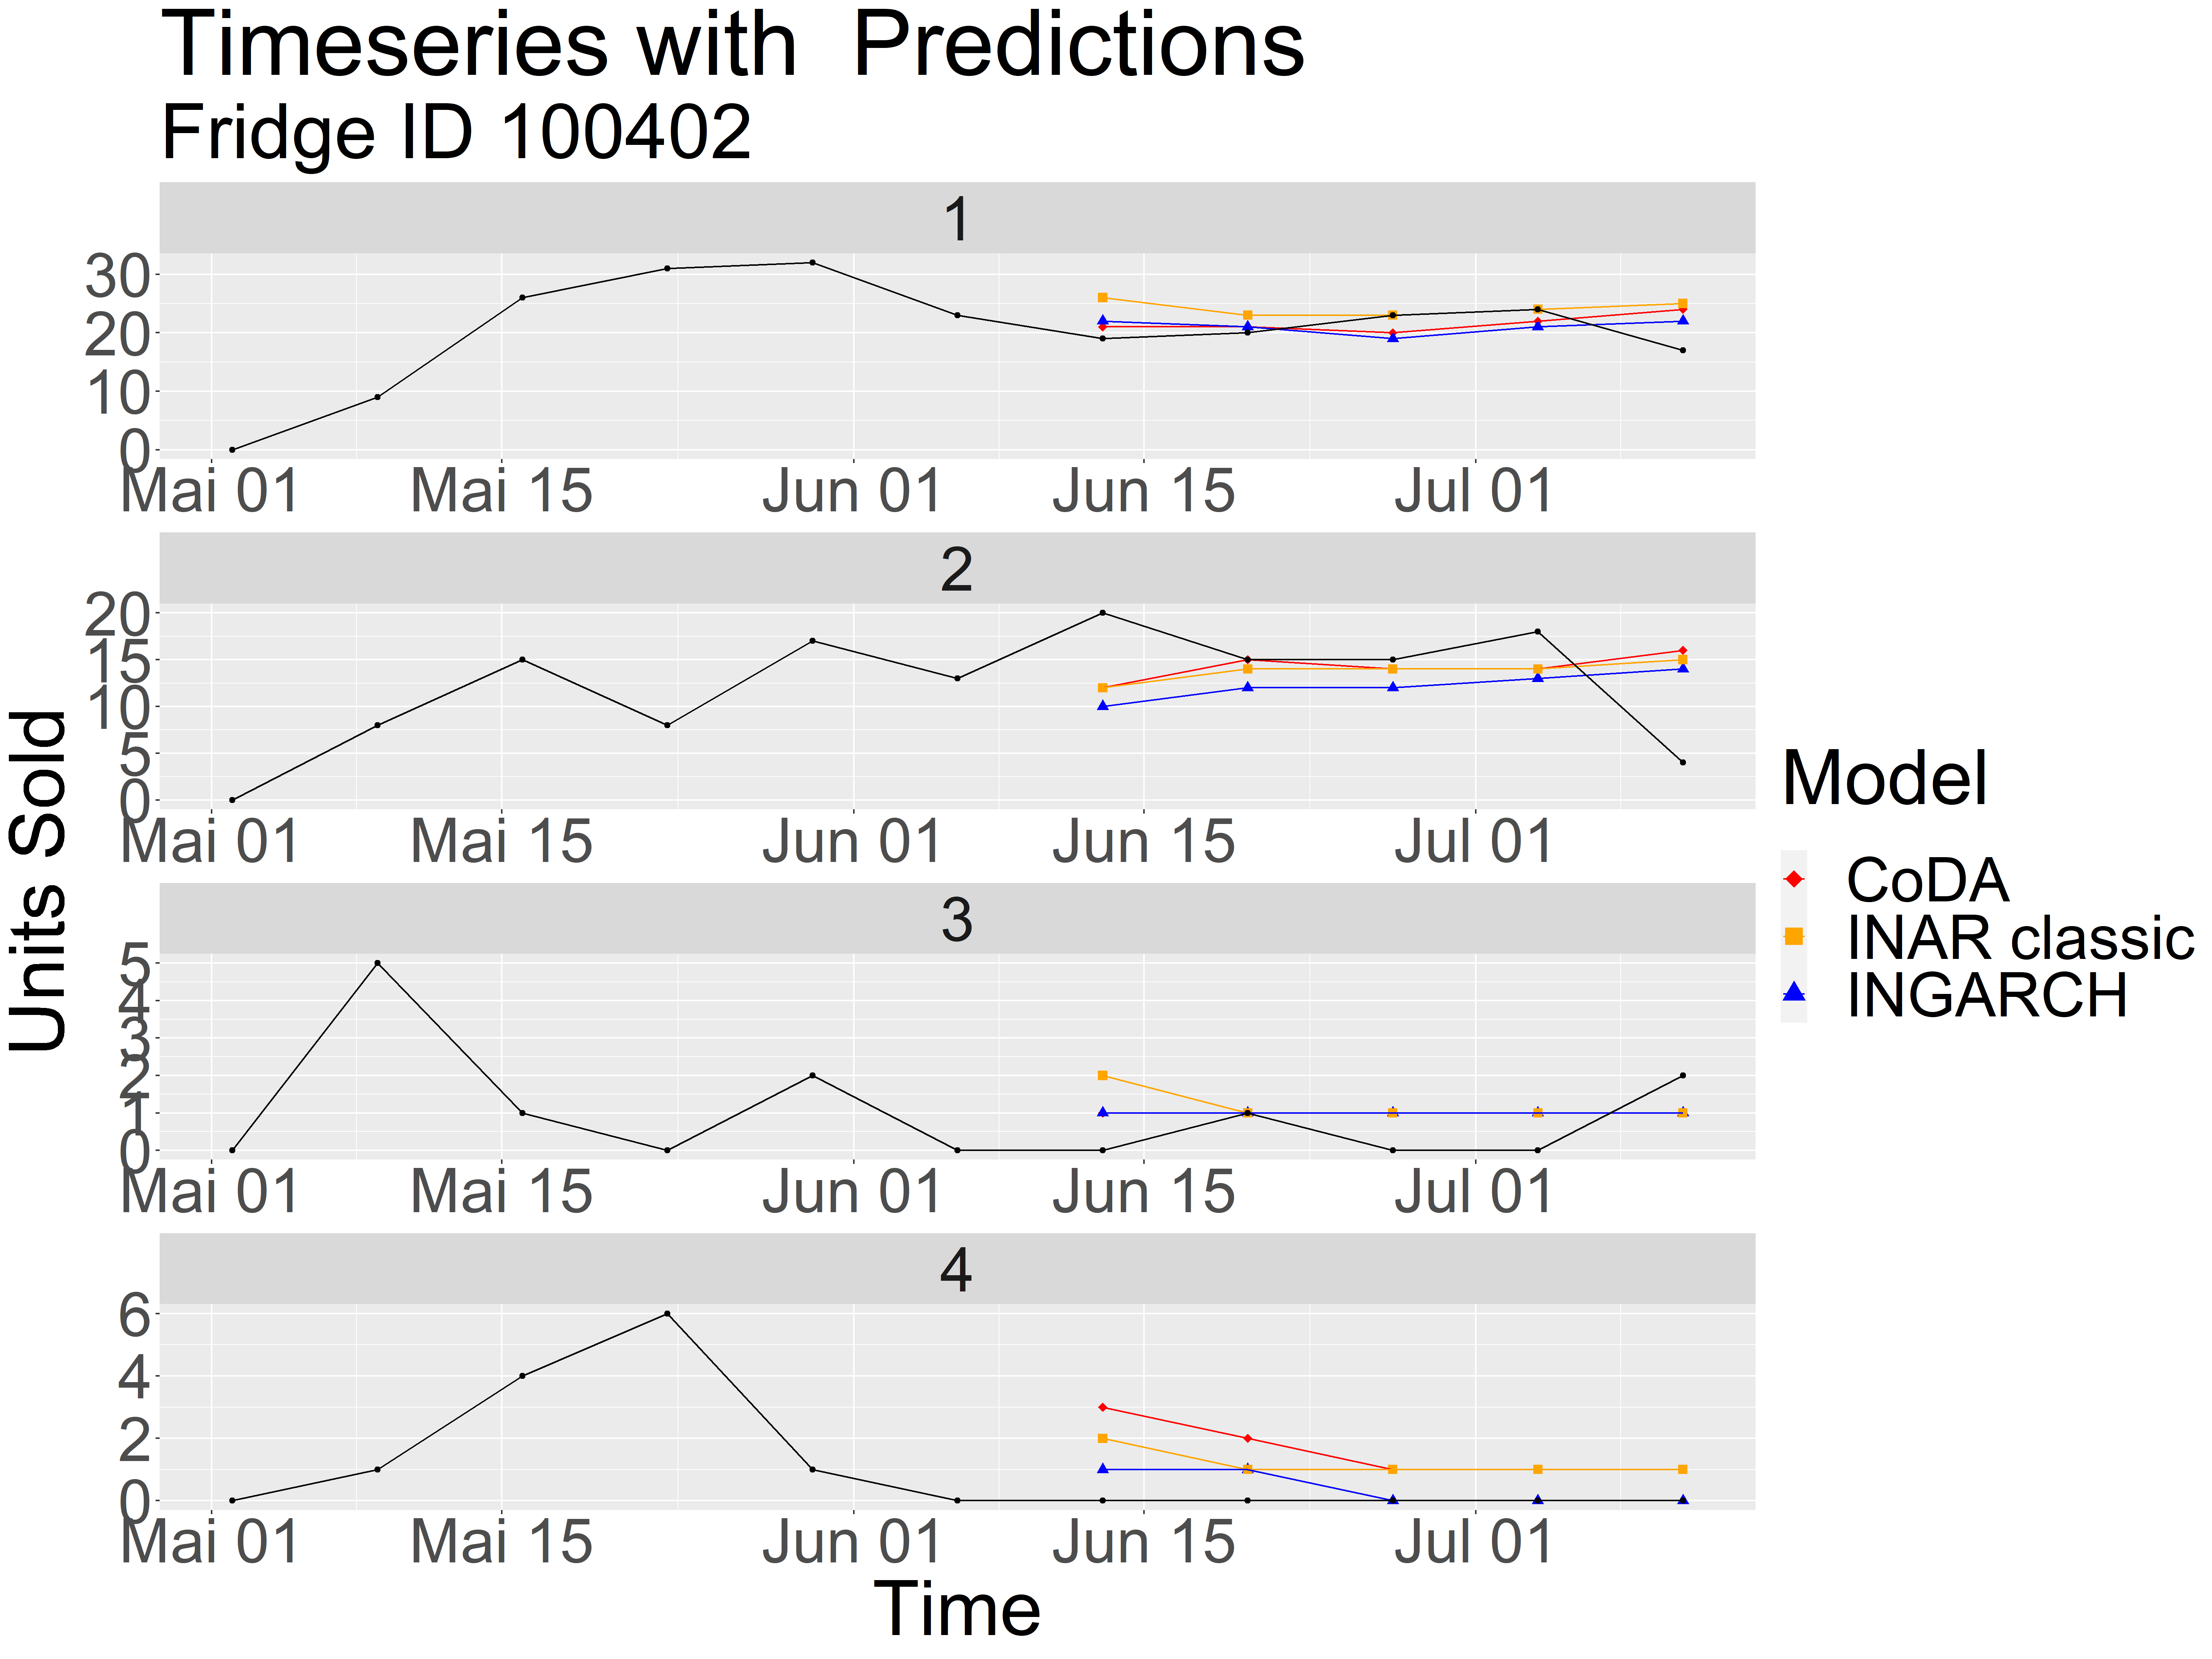
\includegraphics[width=0.80\textwidth]{Graphiken/CodaIngarchInar_Timeseries_ID100402.png}
	%\caption{Time series for fridge 100402}
	%\label{fig:CodaIngarchInar_Timeseries_ID100402}
%\end{figure}
%
%The second highest error for CoDA is for fridge 100403 \ref{fig:CodaIngarchInar_Timeseries_ID100403}. Again, we only have zero values for category 4 but this time non of the methods predicts zero values. The same reasoning as above can be used to explain the high error value. 
%
%\begin{figure}[htbp]
	%\centering
		%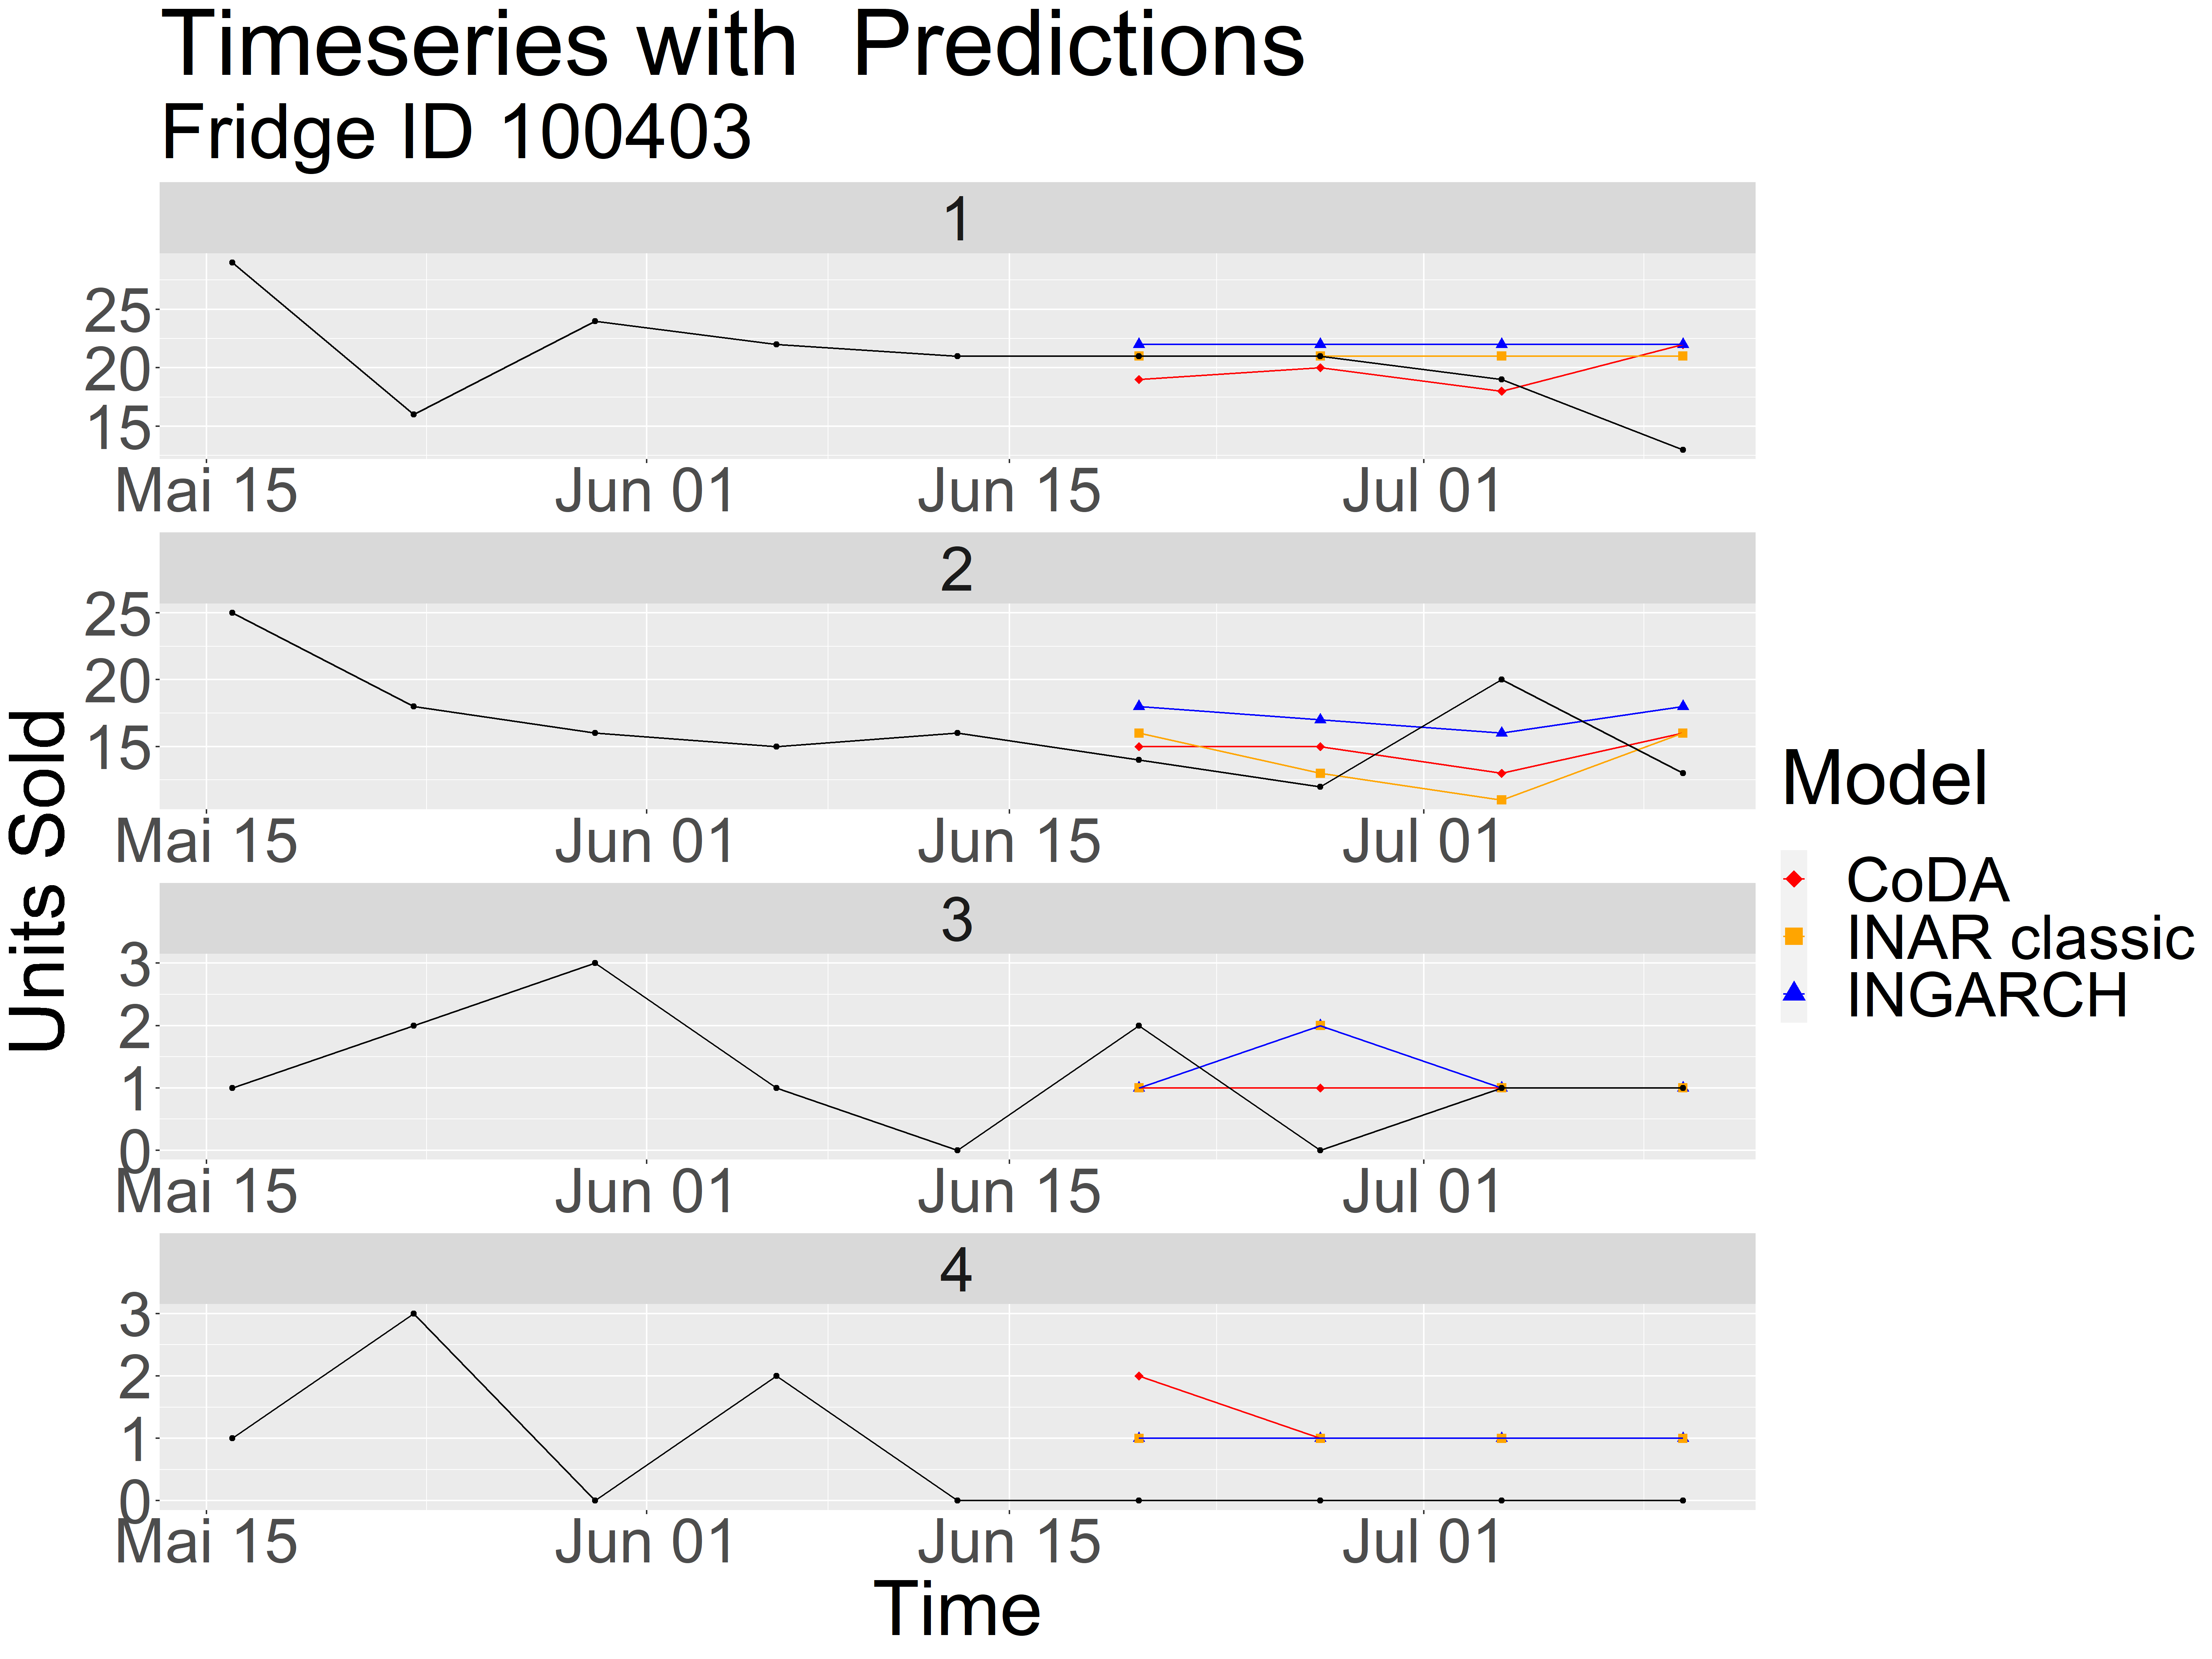
\includegraphics[width=0.80\textwidth]{Graphiken/CodaIngarchInar_Timeseries_ID100403.png}
	%\caption{Time series for fridge 100403}
	%\label{fig:CodaIngarchInar_Timeseries_ID100403}
%\end{figure}
%
%The same thing happens for time series 100191. We have an excessive amount of zero values and CoDA fails to adapt to this while INGARCH and INAR both start to predict zero after some time.
%
%\begin{figure}[htbp]
	%\centering
		%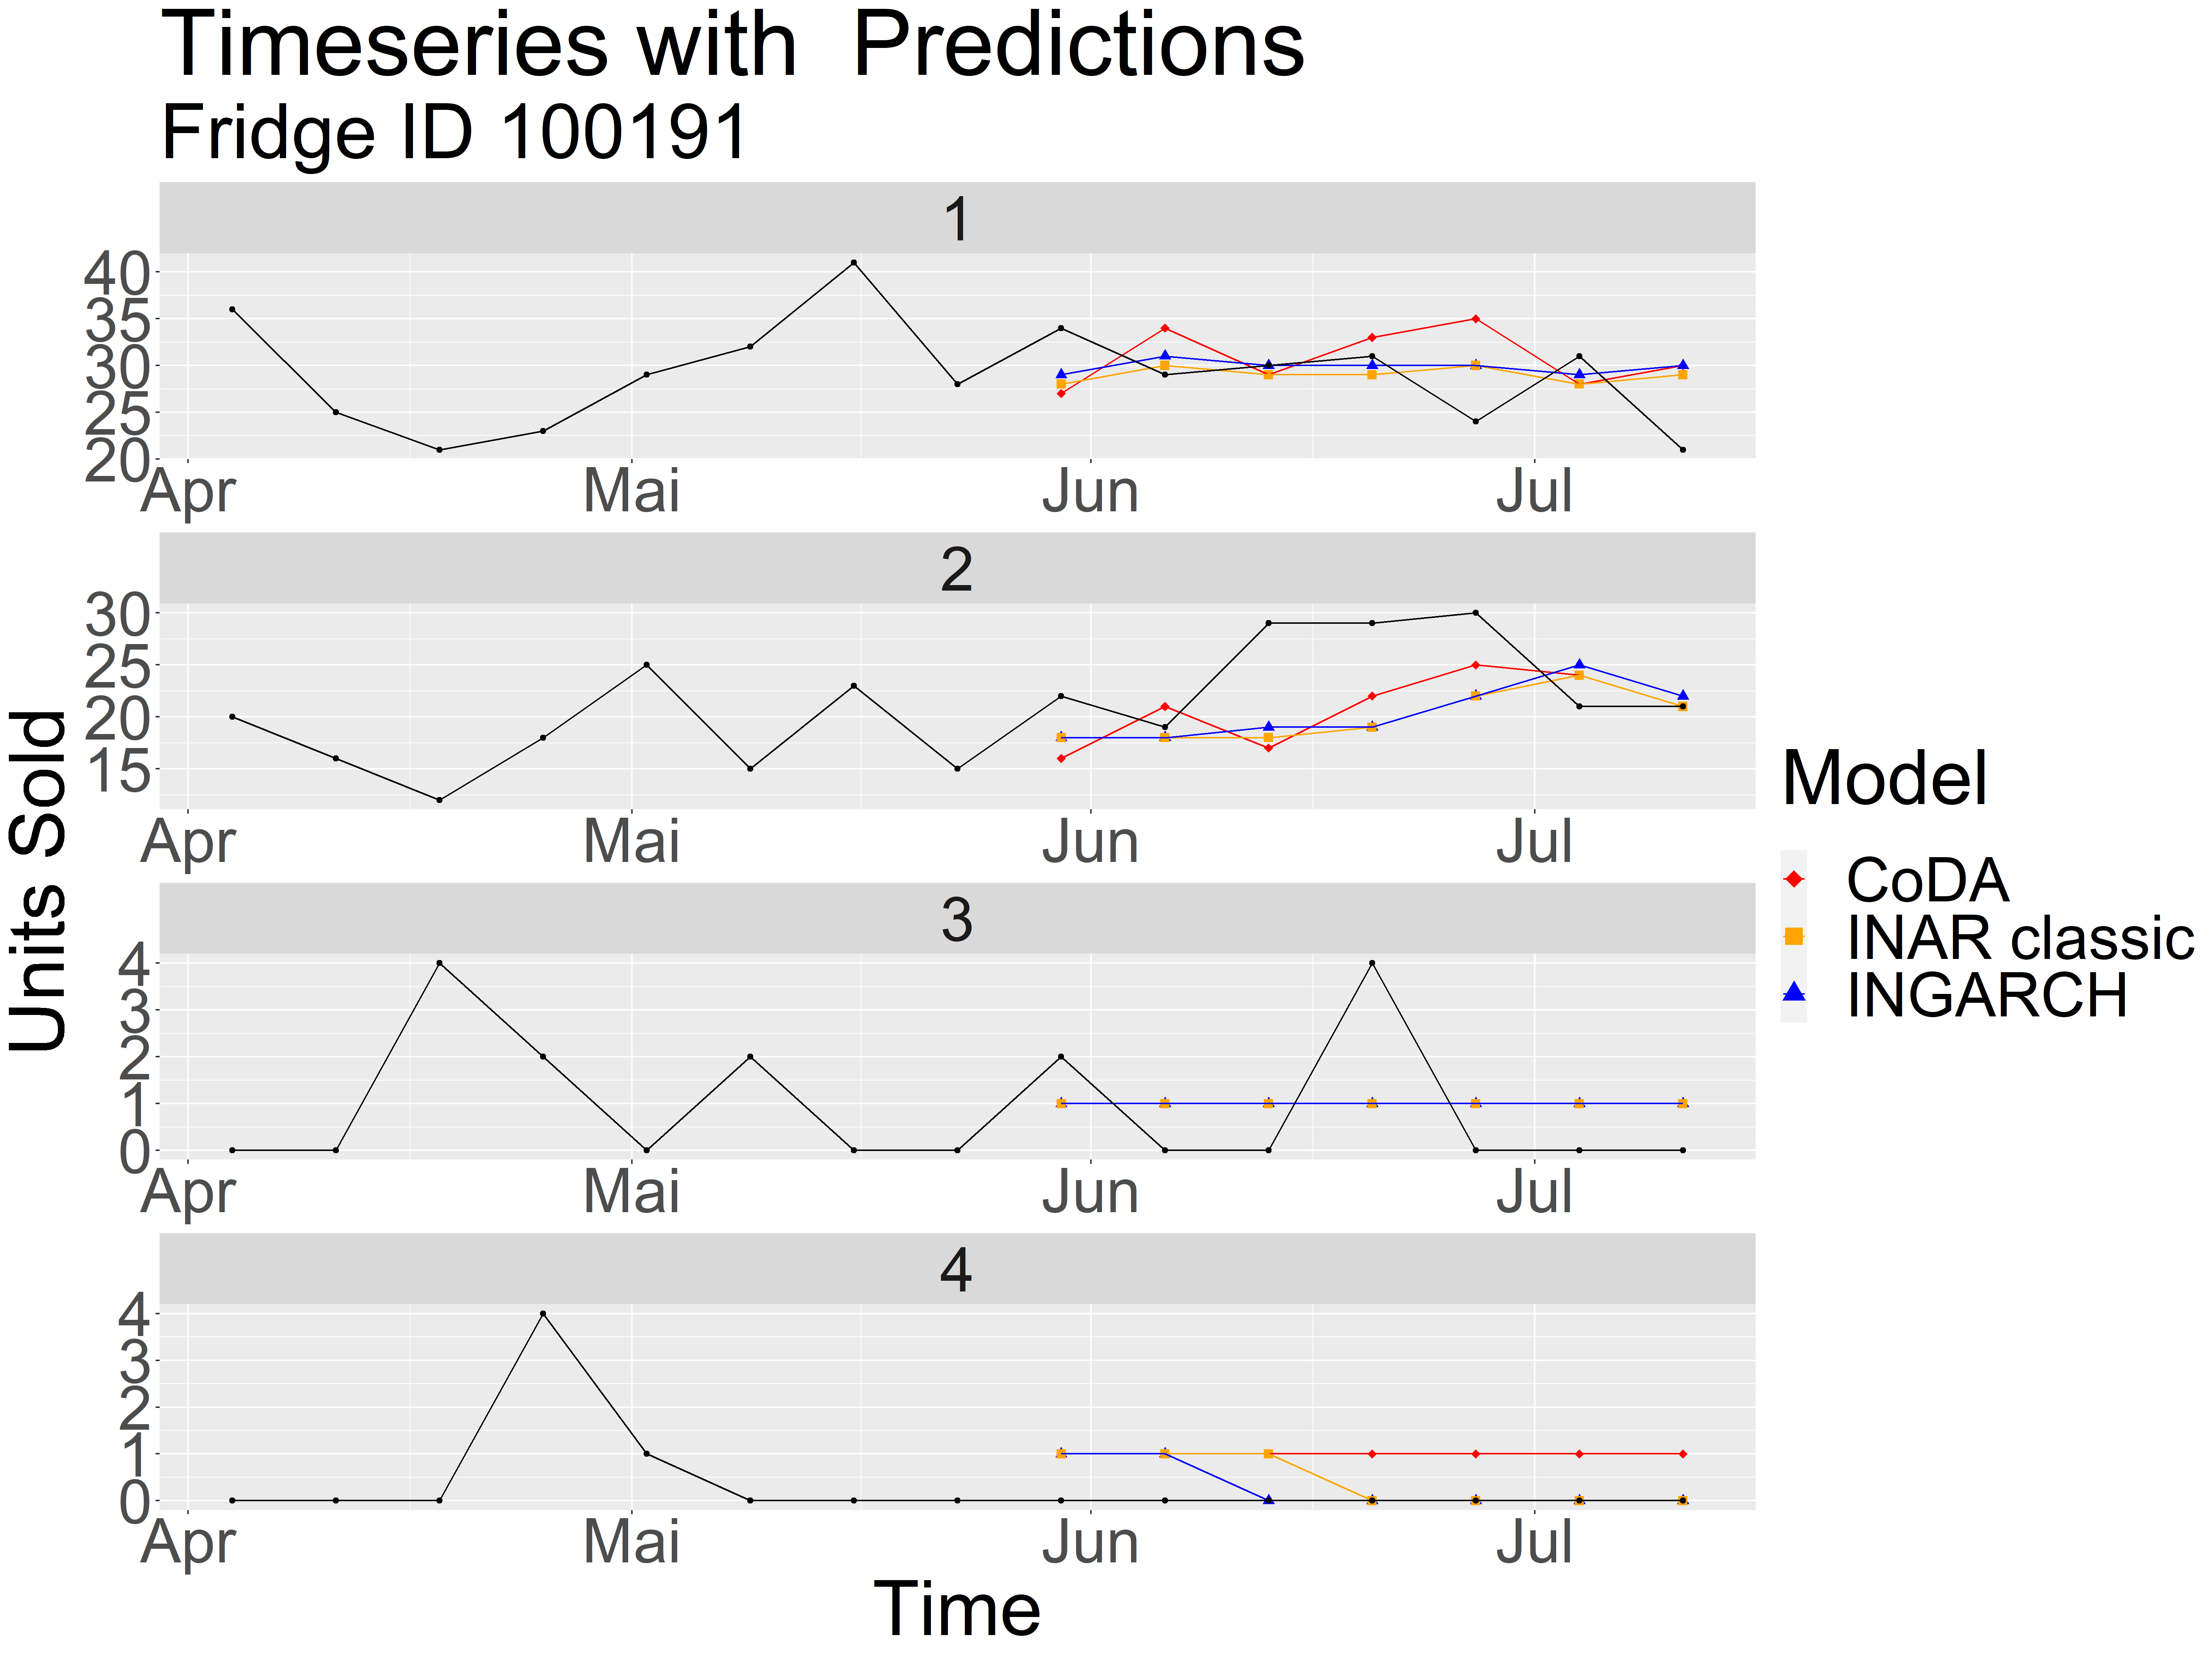
\includegraphics[width=0.80\textwidth]{Graphiken/CodaIngarchInar_Timeseries_ID100191.png}
	%\caption{Time series for fridge 100191}
	%\label{fig:CodaIngarchInar_Timeseries_ID100191}
%\end{figure}
%
%This shows that the CoDA methodolgy seems to struggle with an excessive amount of zero values.

\subsection{General Specifications}
\label{sec:General Specifications}

First, we start with specifications which can be chosen for both CoDA and INGARCH. We will always vary one parameter, while using the respective standard values for the other parameters. 
\subsubsection{History}
\label{sec:History}

As mentioned various times throughout this thesis, the the history is one of the parameters which can be adjusted. In figure \ref{fig:History Comp1} we visualise the results as a boxplot, a quantile plot  and additionally an histogram to get a feeling for the error distribution. 

\begin{figure}[htb!]
\centering
\begin{subfigure}[b]{0.45\textwidth}
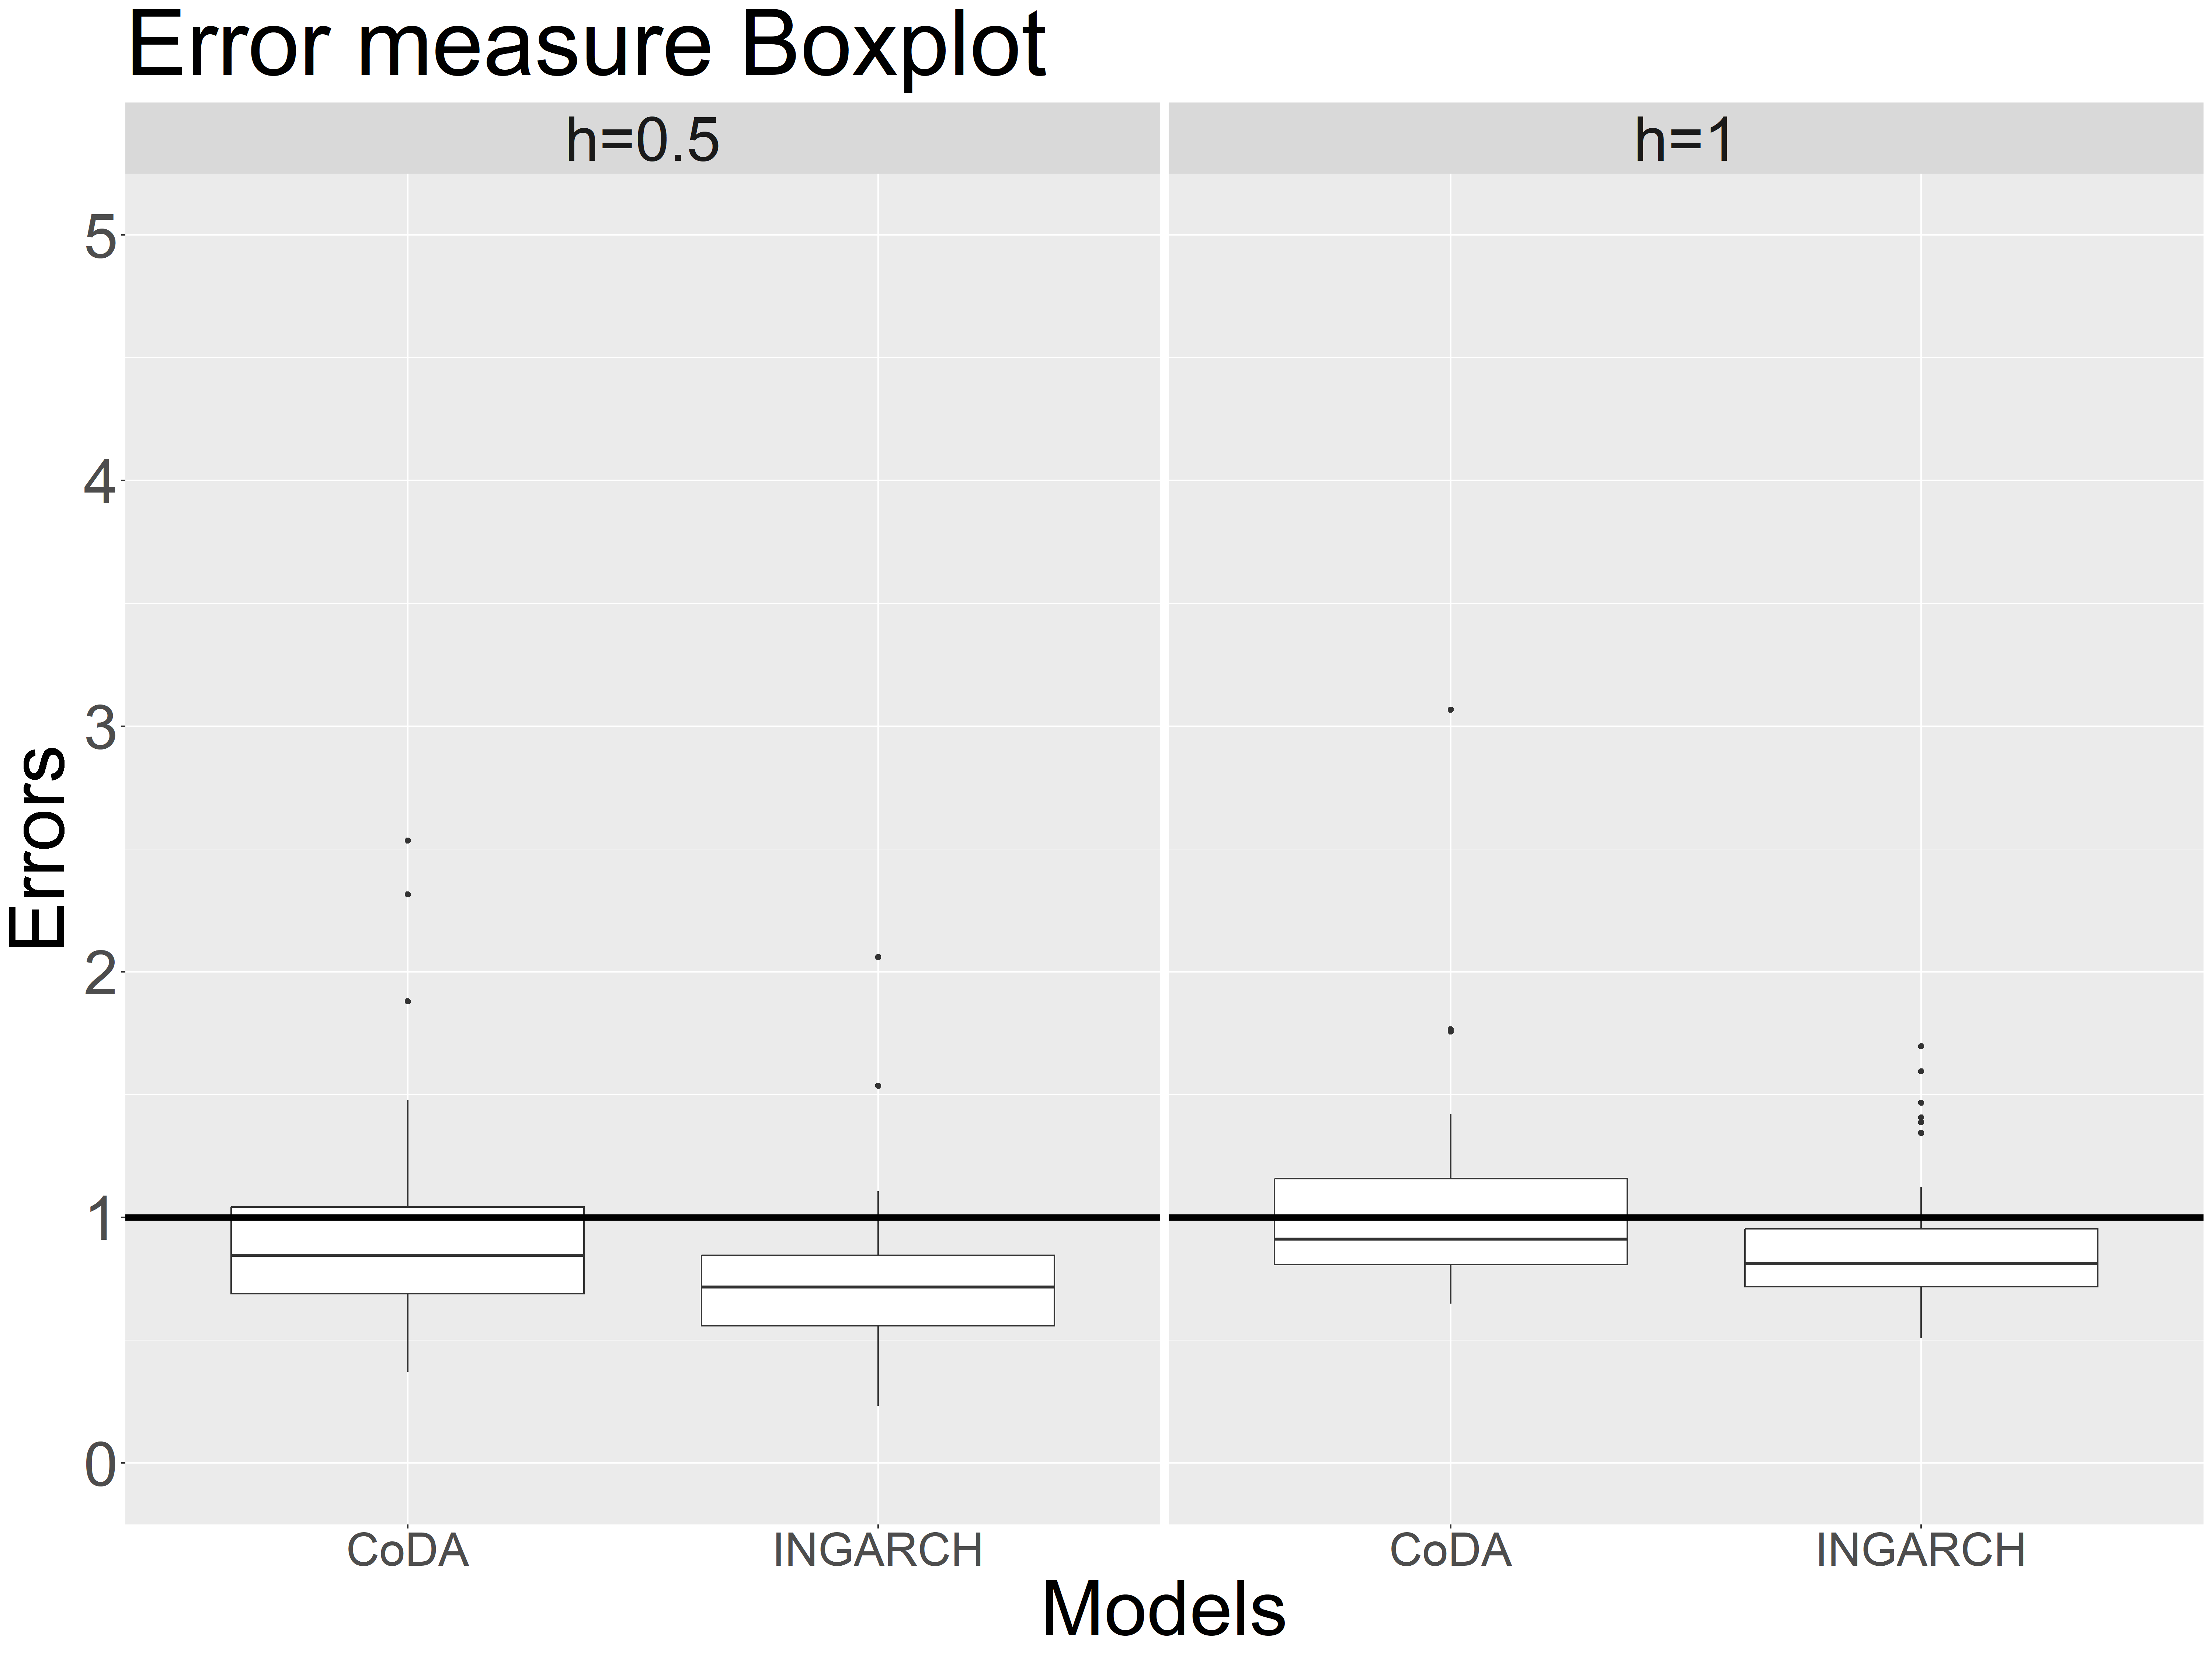
\includegraphics[width=\textwidth]{ErrorMeasureCombined_Box_all__Variation_history.png}
\caption{Boxplot of different $h$}
\label{fig:History Box}
\end{subfigure}
\hfill
\begin{subfigure}[b]{0.45\textwidth}
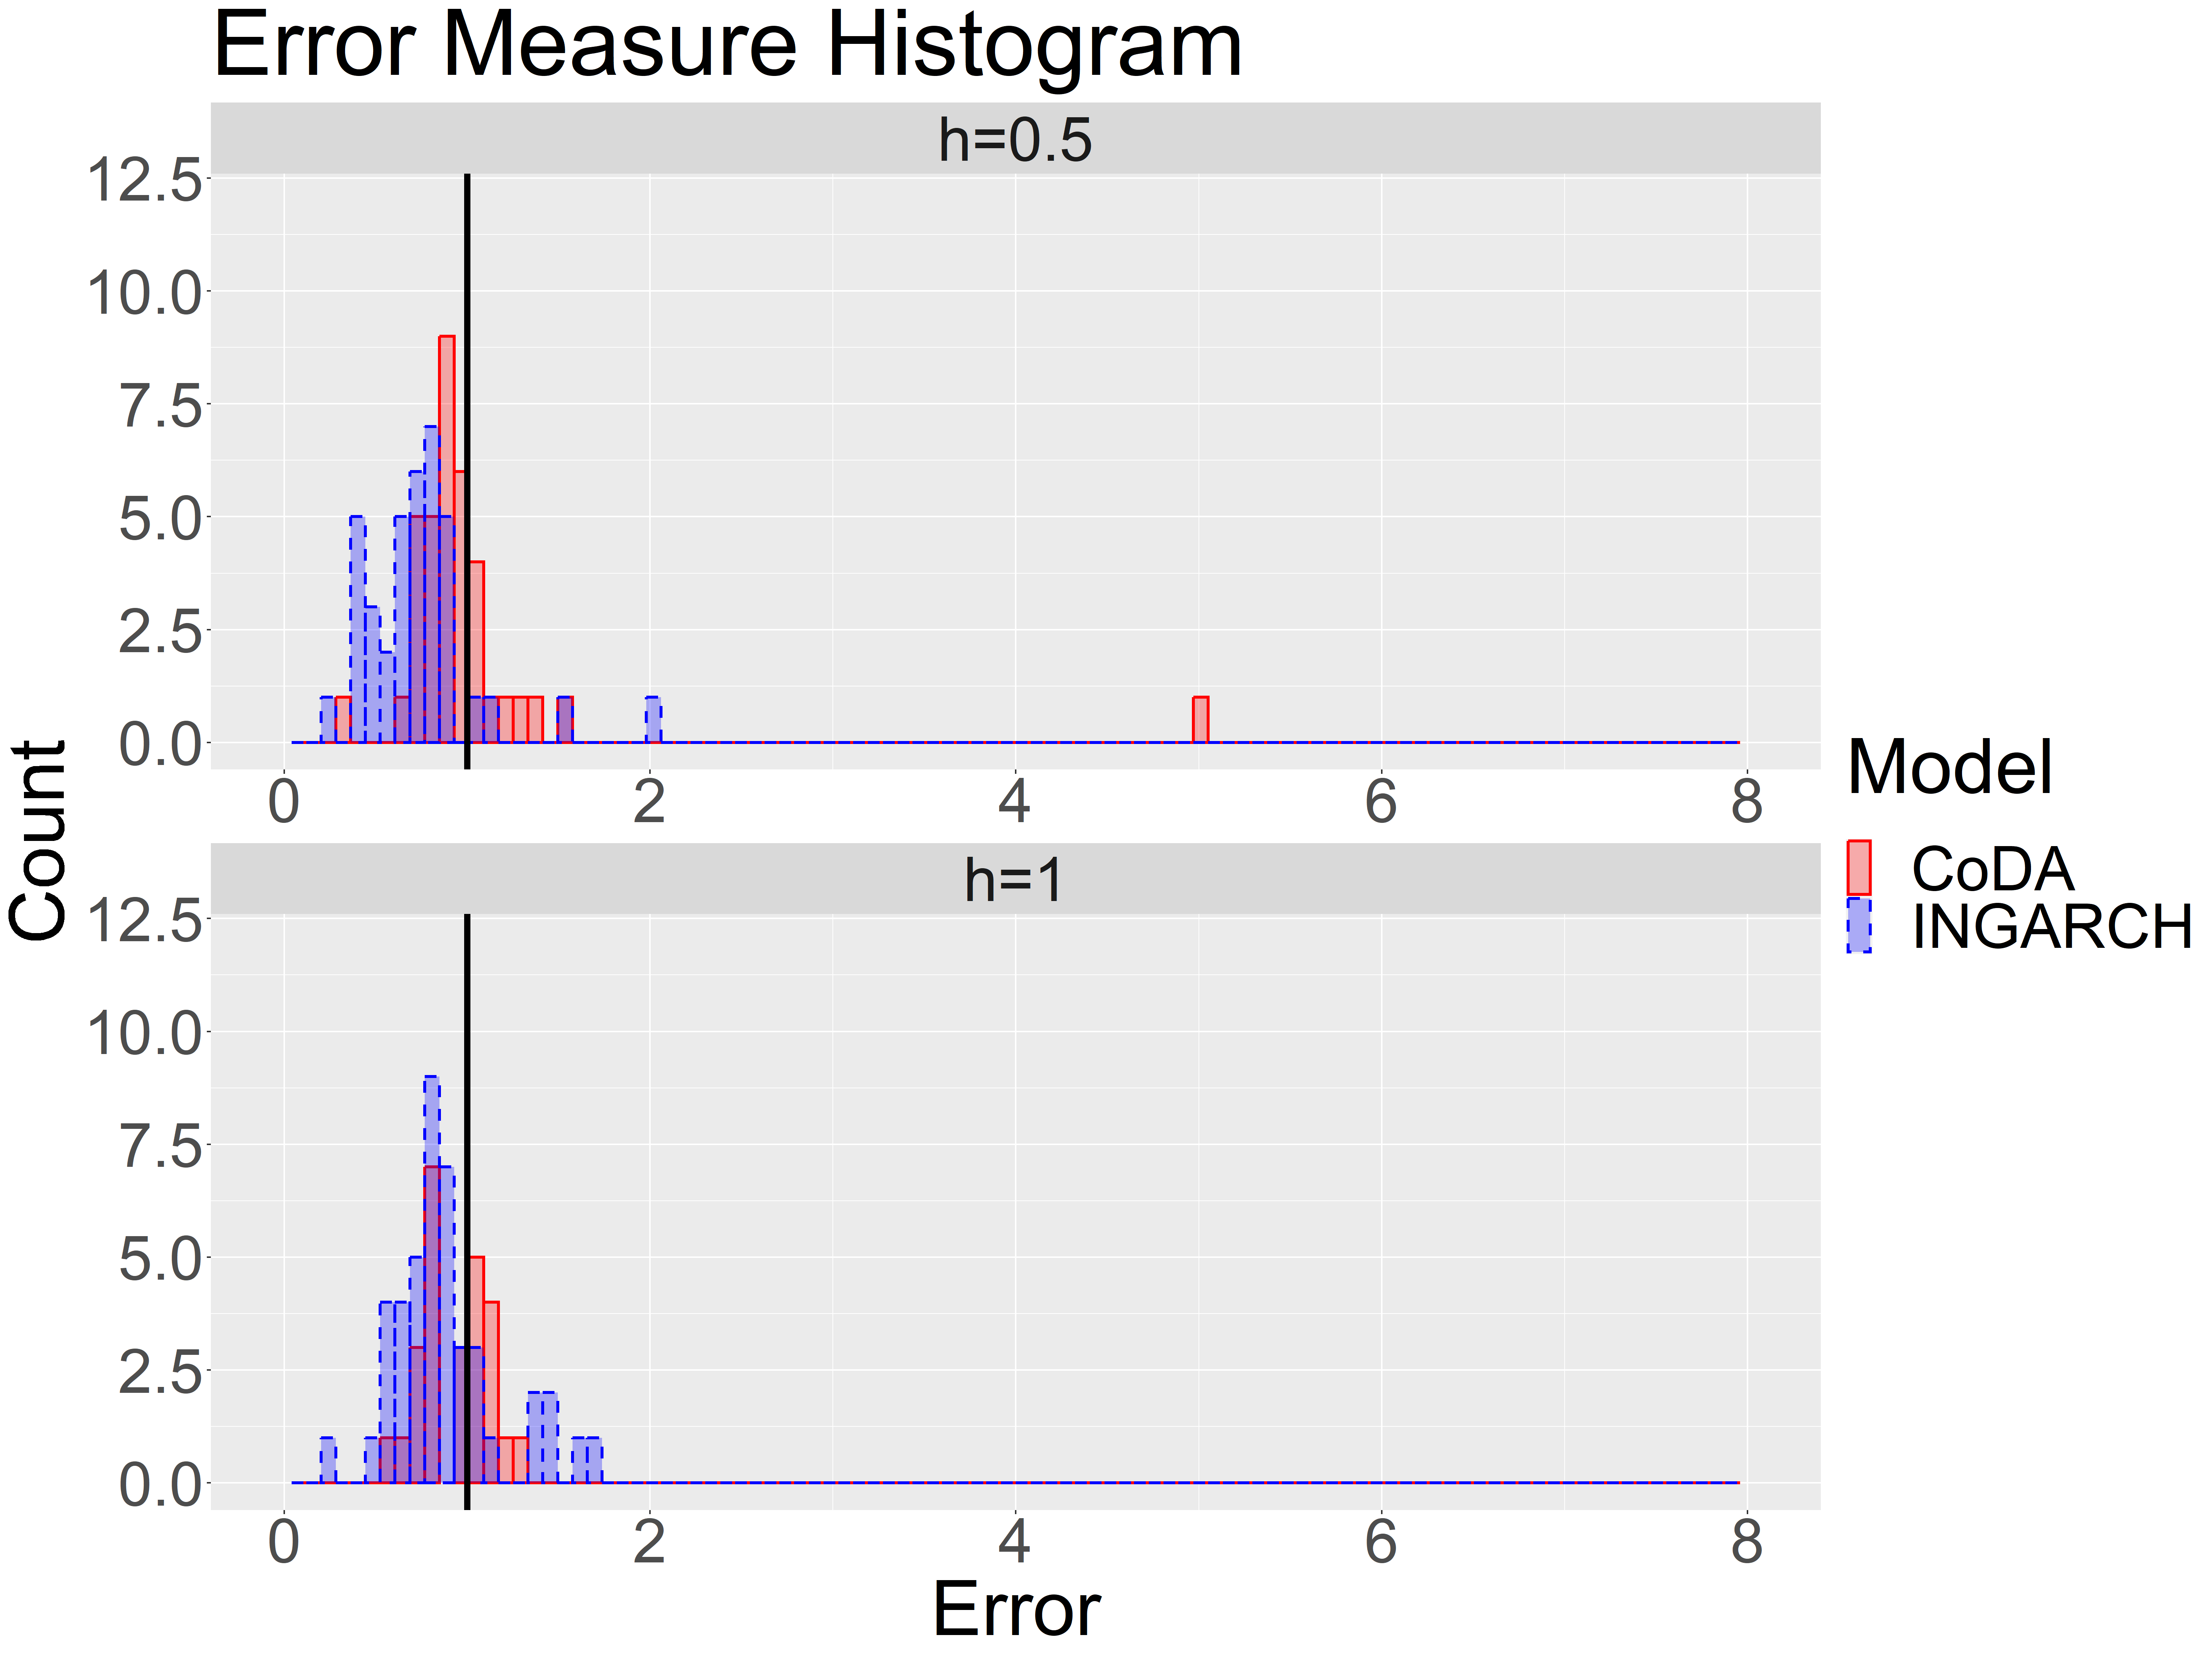
\includegraphics[width=\textwidth]{ErrorMeasureCombined_Histogram_all__Variation_history.png}
\caption{Histogram of different $h$}
\label{fig:History Hist}
\end{subfigure}
\hfill
\begin{subfigure}[b]{0.8\textwidth}
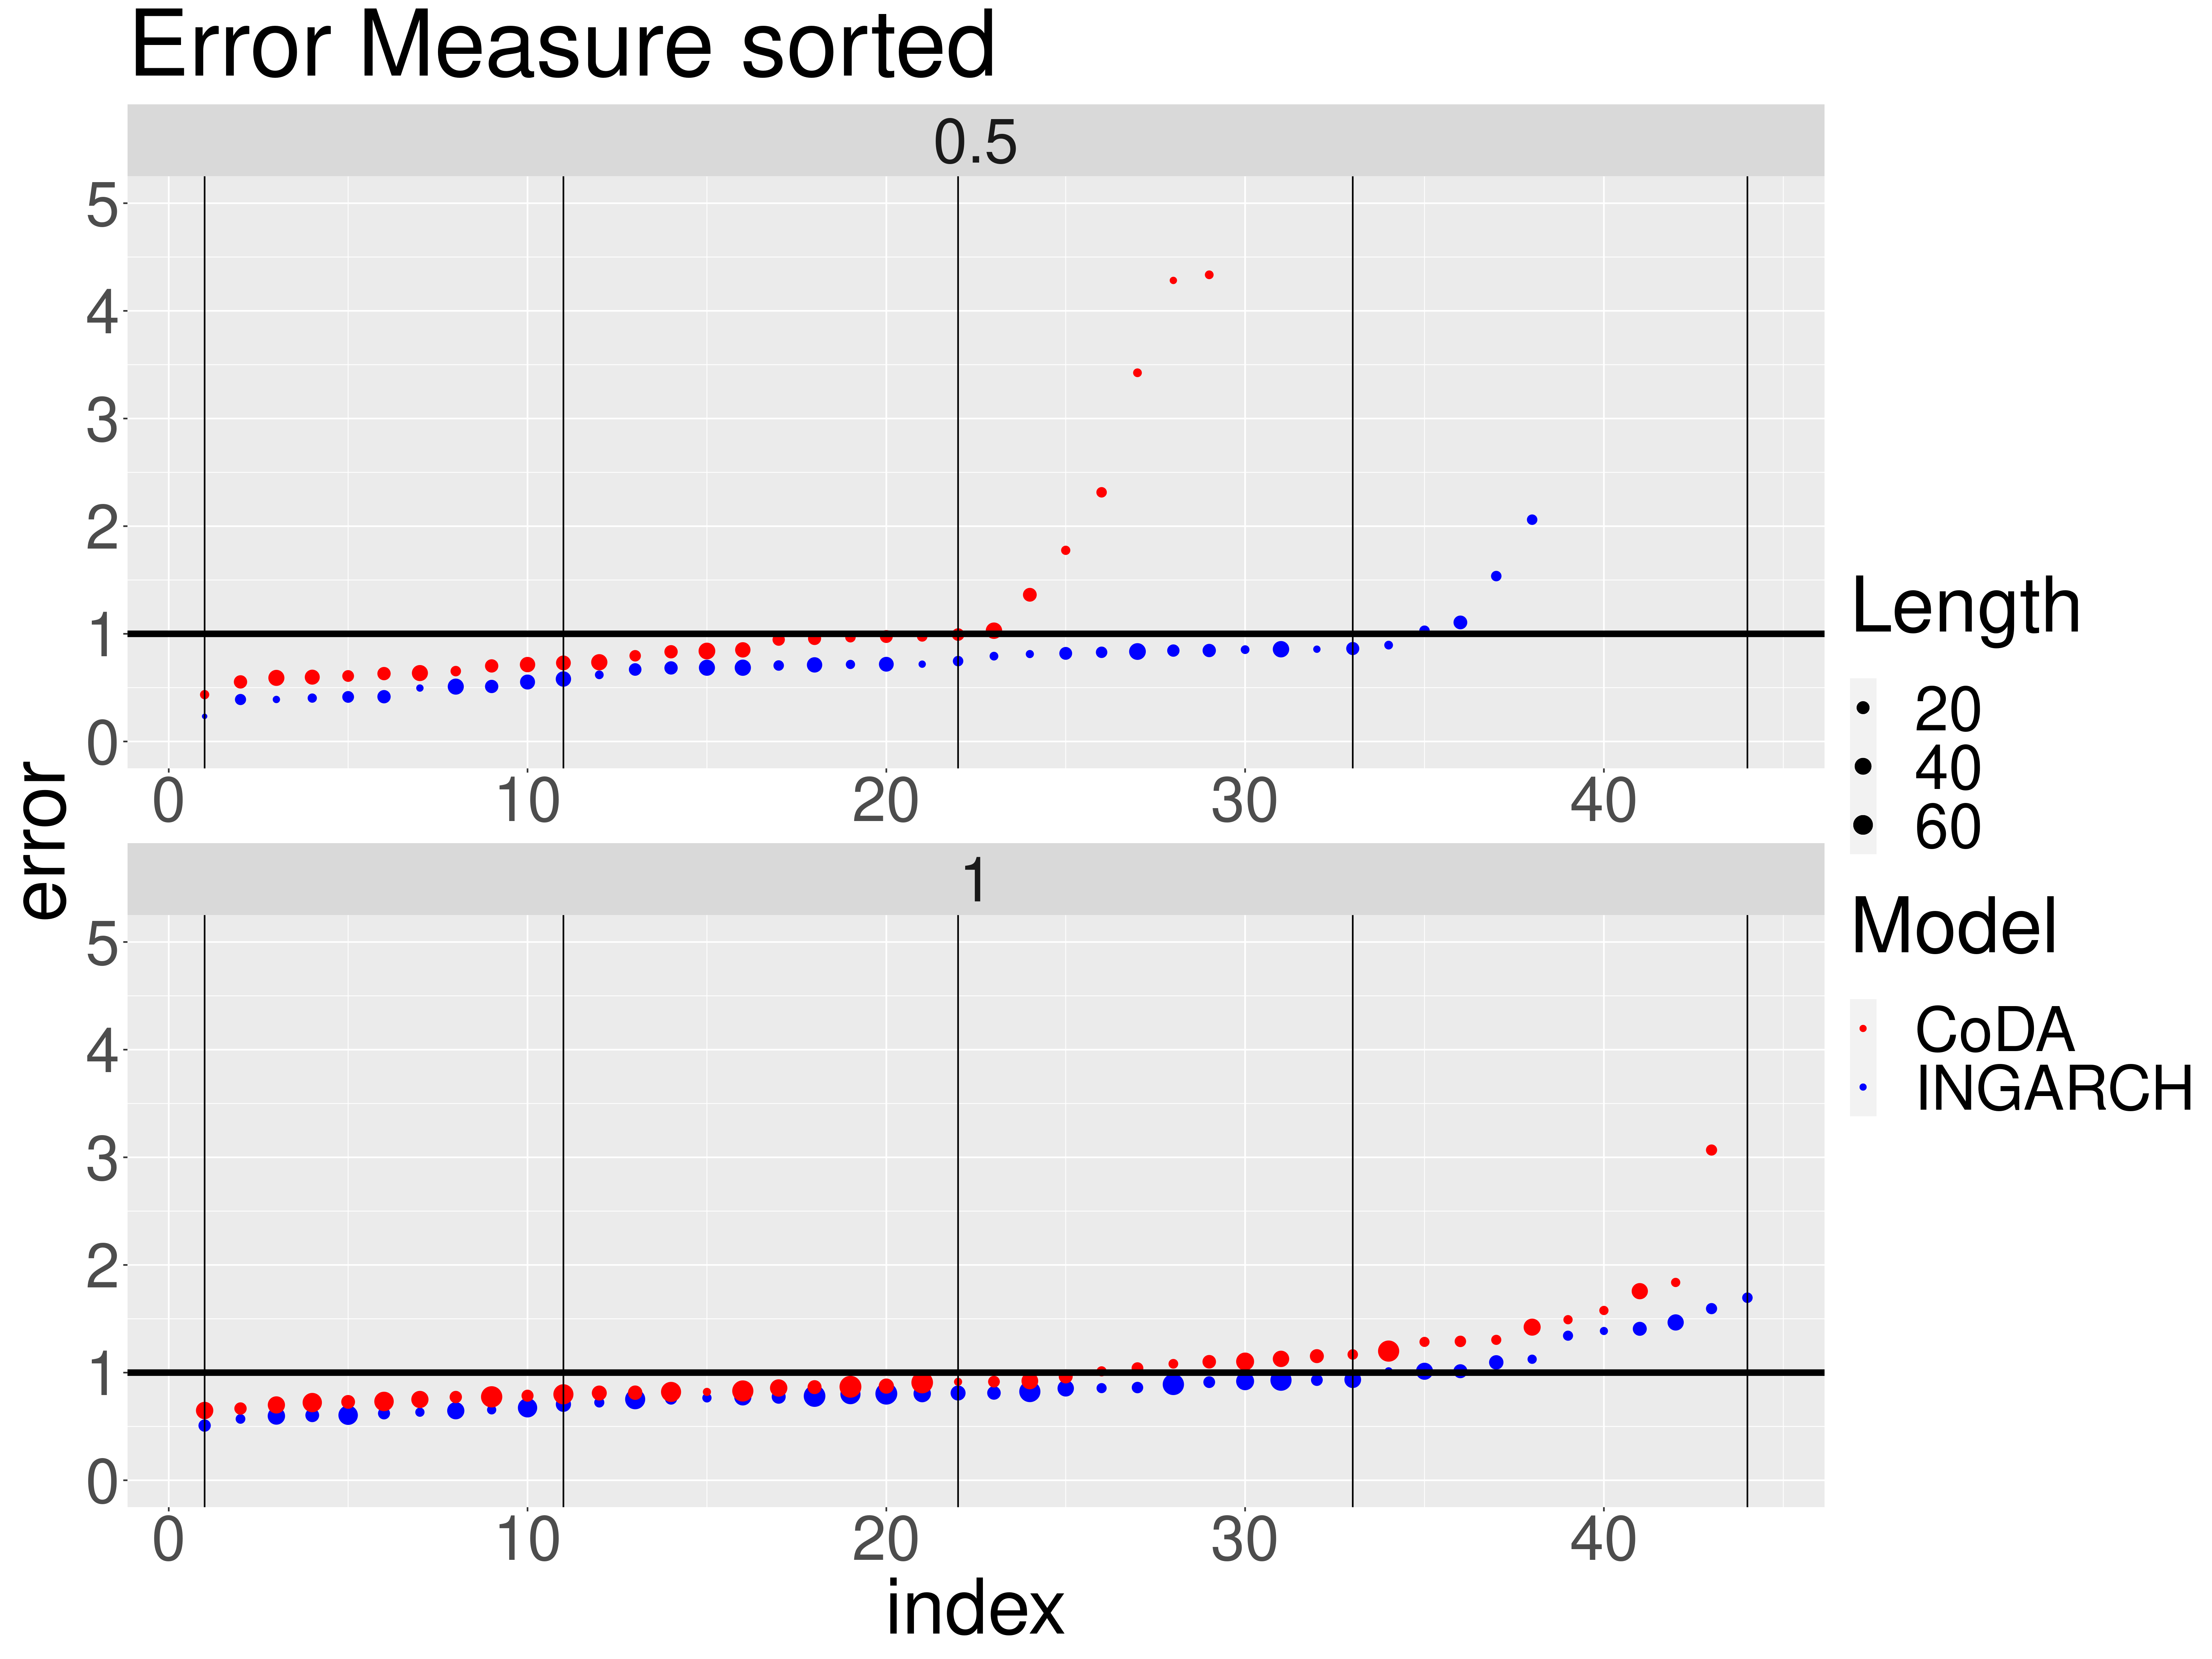
\includegraphics[width=\textwidth]{ErrorMeasureCombined_Quant_all__Variation_history.png}
\caption{Quantiles Plot of different $h$}
\label{fig:History Quant}
\end{subfigure}
\caption{Comparison of different $h$}
\label{fig:History Comp1}
\end{figure}

In figure \ref{fig:History Comp1} we can see that the results for CoDA do not vary too much for the different histories. However, one can see in the quantile plot \ref{fig:History Quant} that we have 8 less values for  $h=0.5$ than for $h=1$. This probably results from the fact, that if we only take half of the history for an already short time series, then we have too little values for estimating. 

For INGARCH, the results are similar as well. For $h=1$ we get slightly higher values for the error measure as seen in \ref{fig:History Box}. But again in \ref{fig:History Quant} we see that we have less values for the shorter history for the same reason as above. 

\subsubsection{Frame}
\label{sec:Frame}

Next, we vary the initial frame length $w_f$. We choose to extend the frame with each new data point. For this we vary the value $w$ in $w_f=w\cdot T$. The results are portrayed in \ref{fig:Frame Comp1}. In general, there is not much difference between the different frames. INGARCH seems to perform better for all three values.
\begin{figure}[htb!]
\centering
\begin{subfigure}[b]{0.45\textwidth}
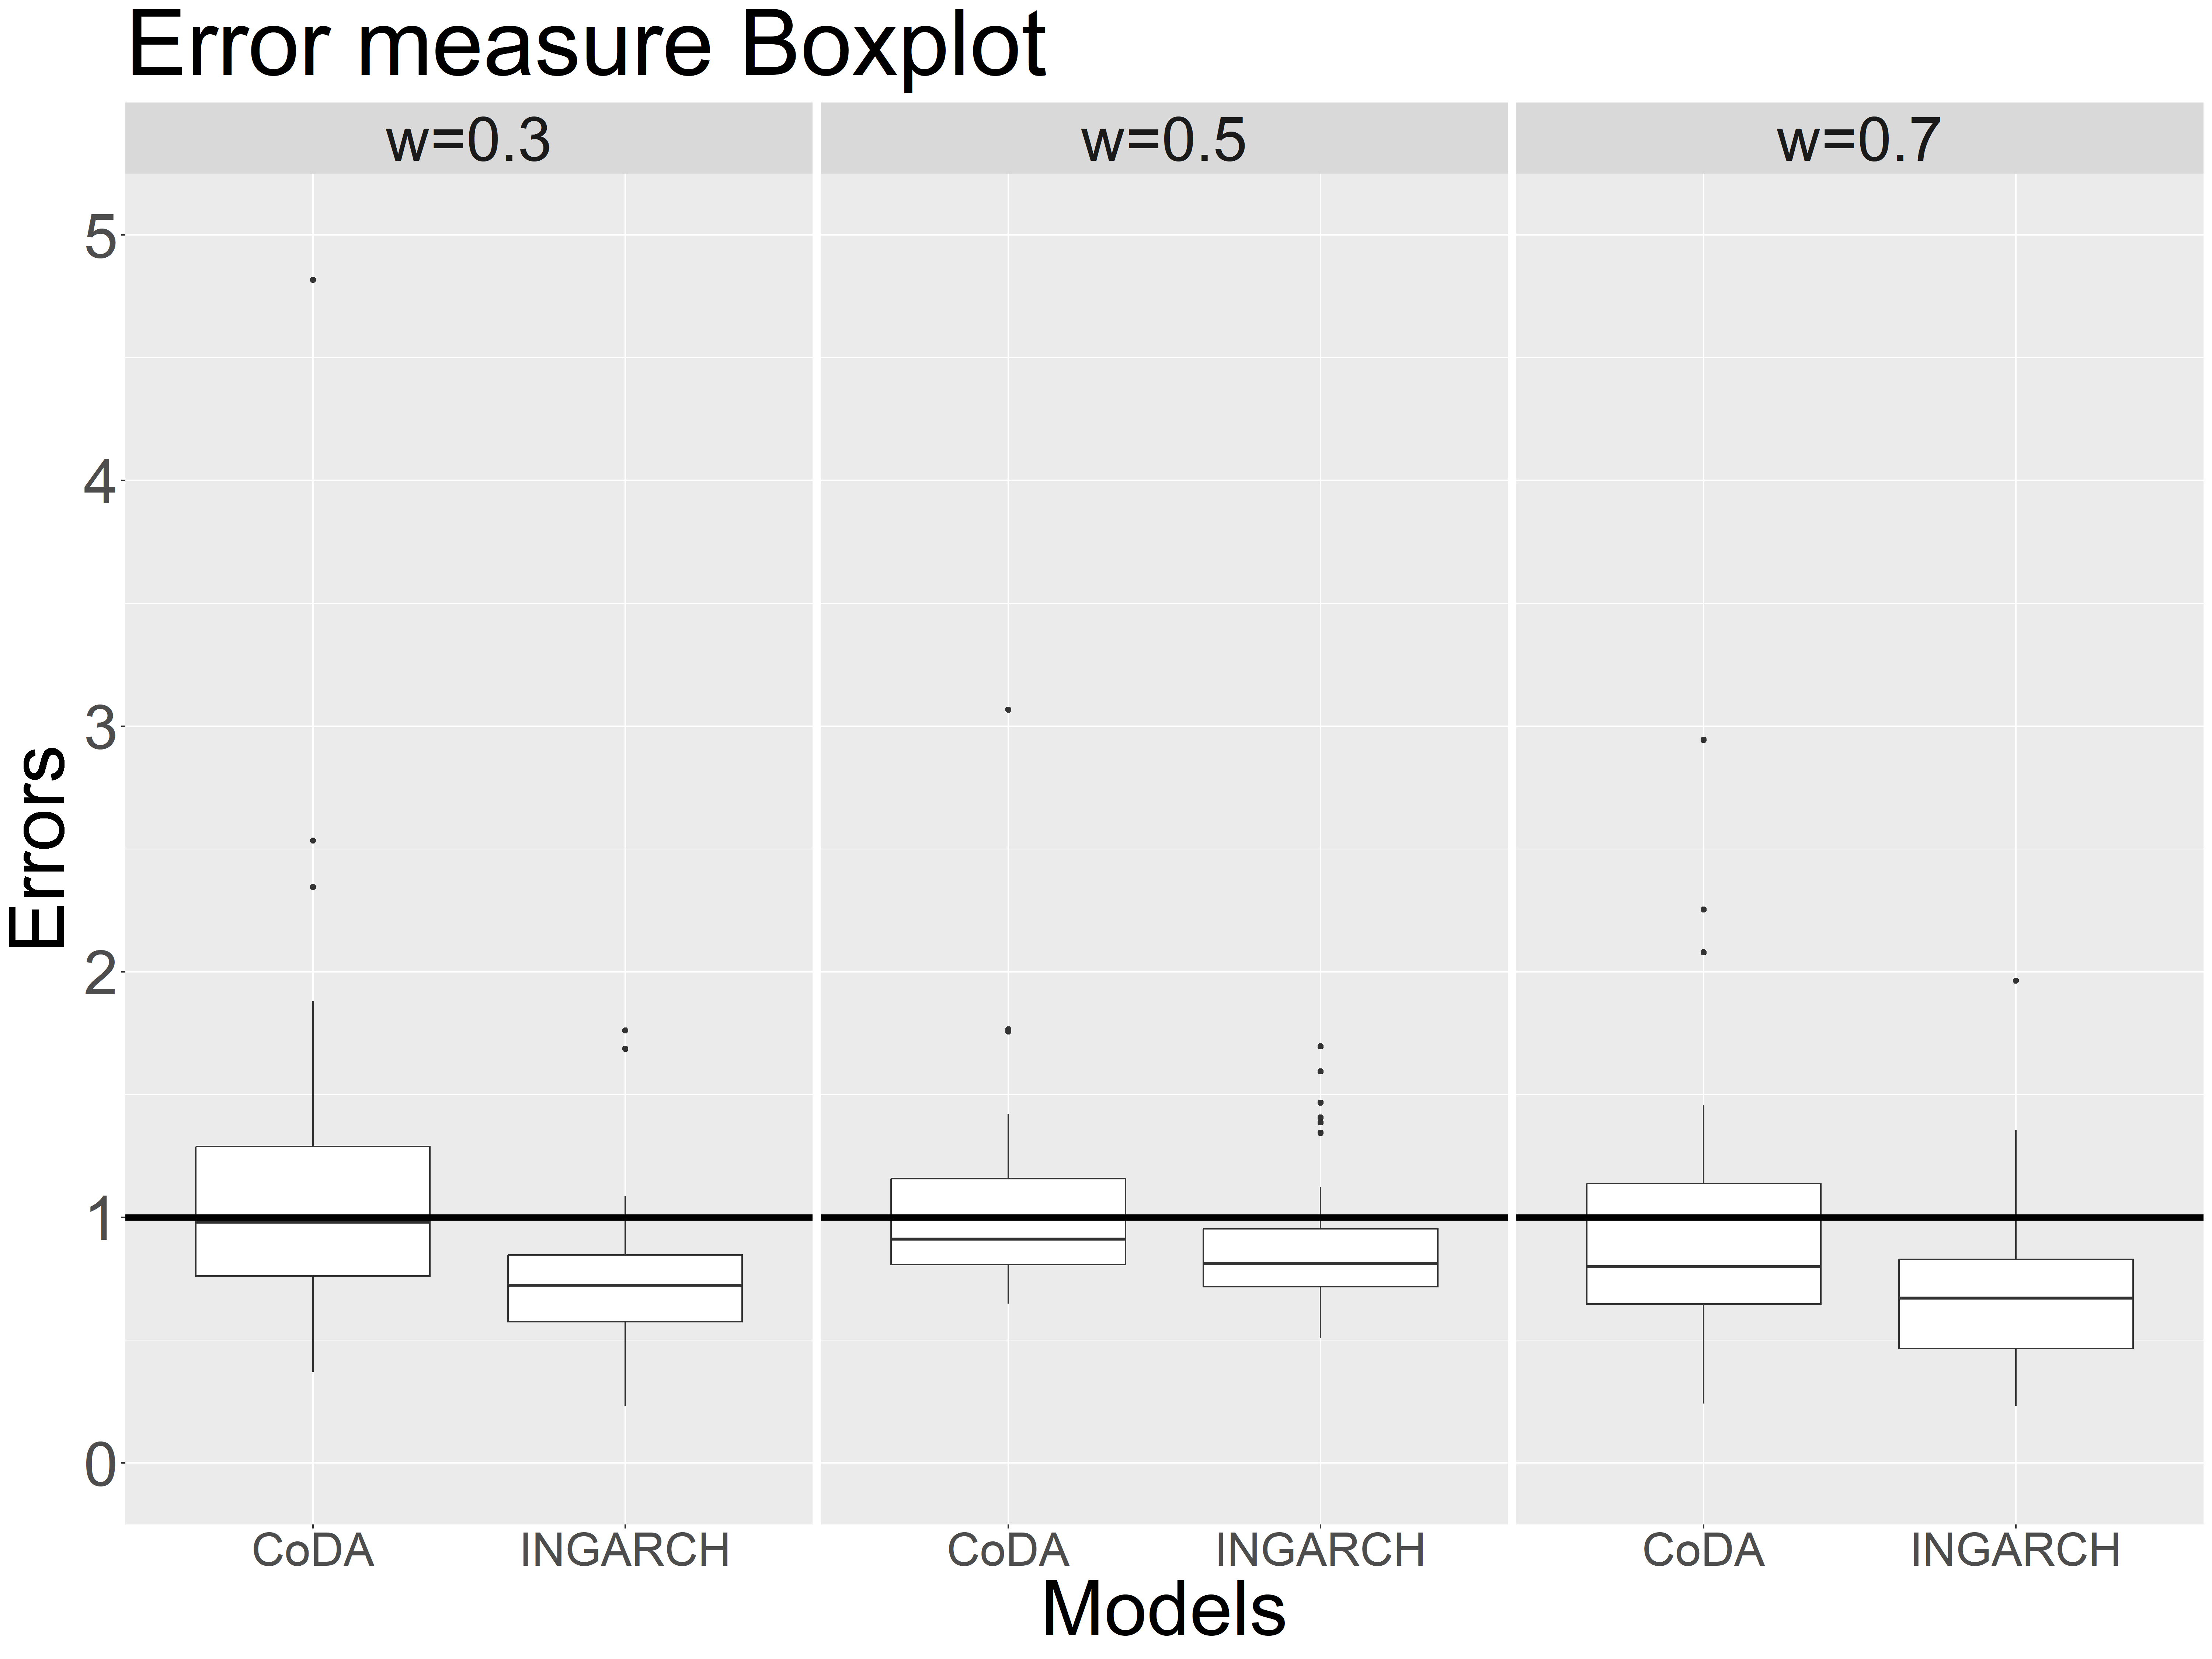
\includegraphics[width=\textwidth]{ErrorMeasureCombined_Box_all__Variation_frame.png}
\caption{Boxplot of different $w$}
\label{fig:Frame Box}
\end{subfigure}
\hfill
\begin{subfigure}[b]{0.45\textwidth}
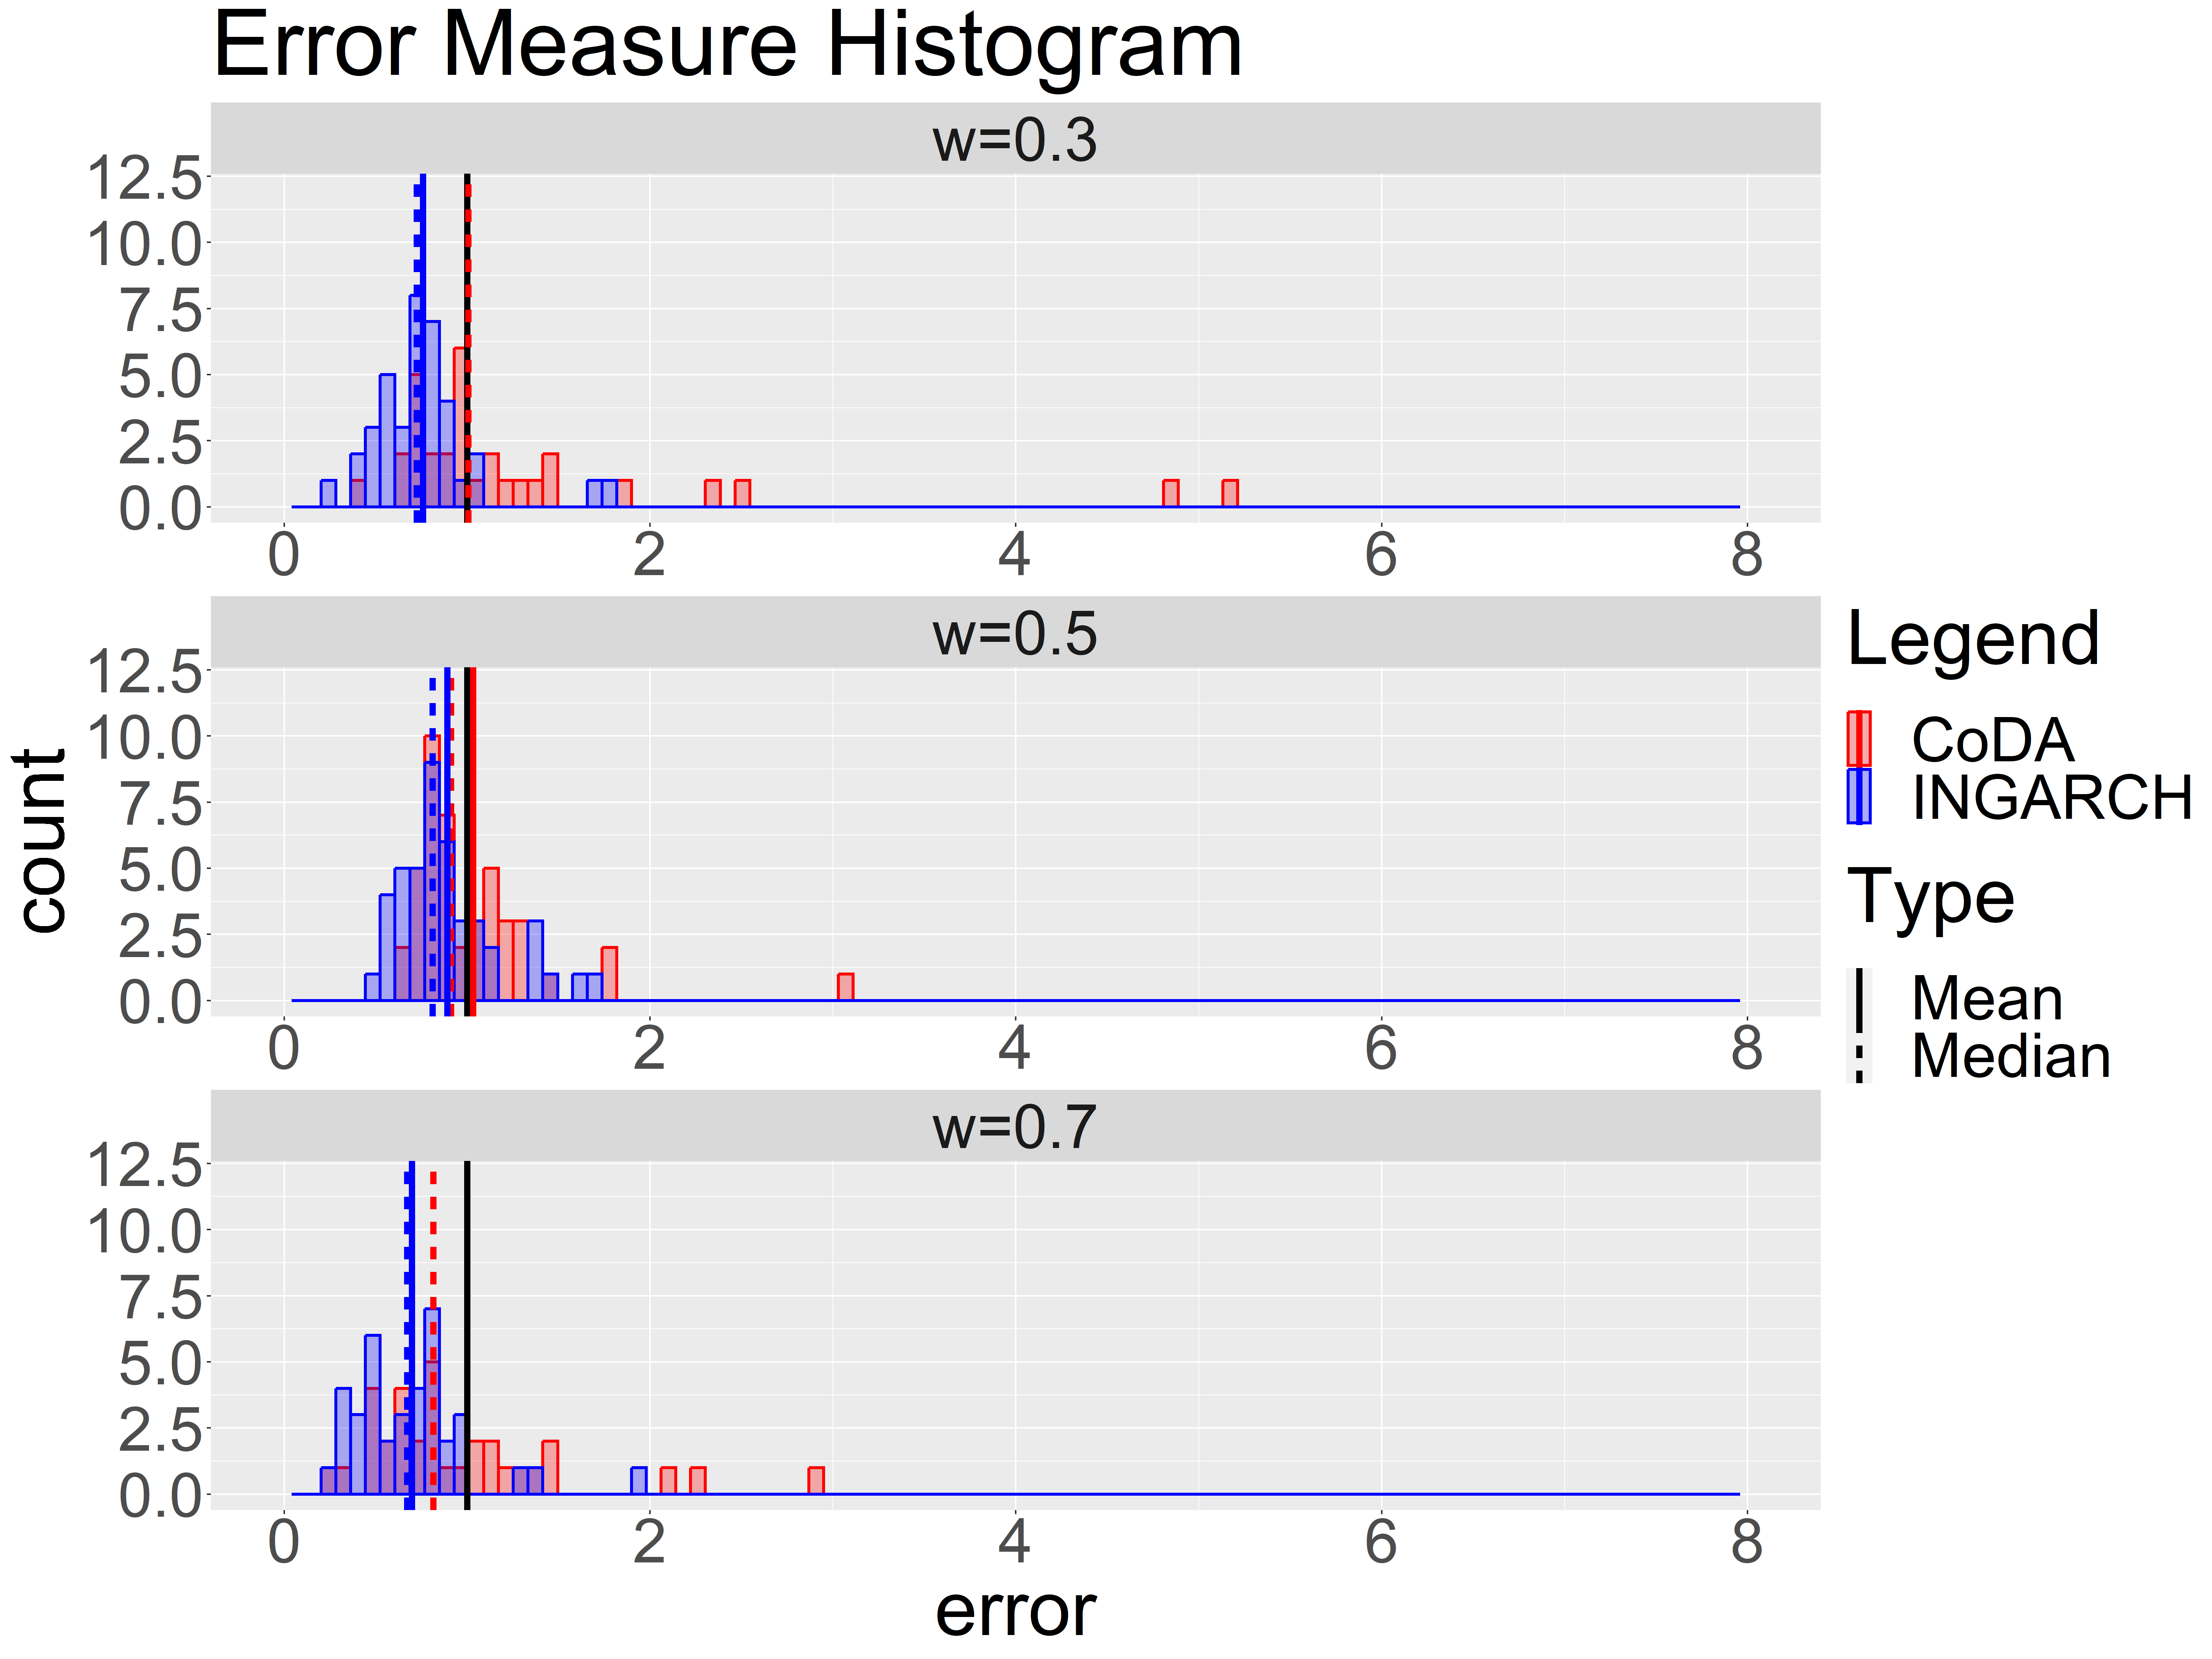
\includegraphics[width=\textwidth]{ErrorMeasureCombined_Histogram_all__Variation_frame.png}
\caption{Histogram of different $w$}
\label{fig:Frame Hist}
\end{subfigure}
\hfill
\begin{subfigure}[b]{0.8\textwidth}
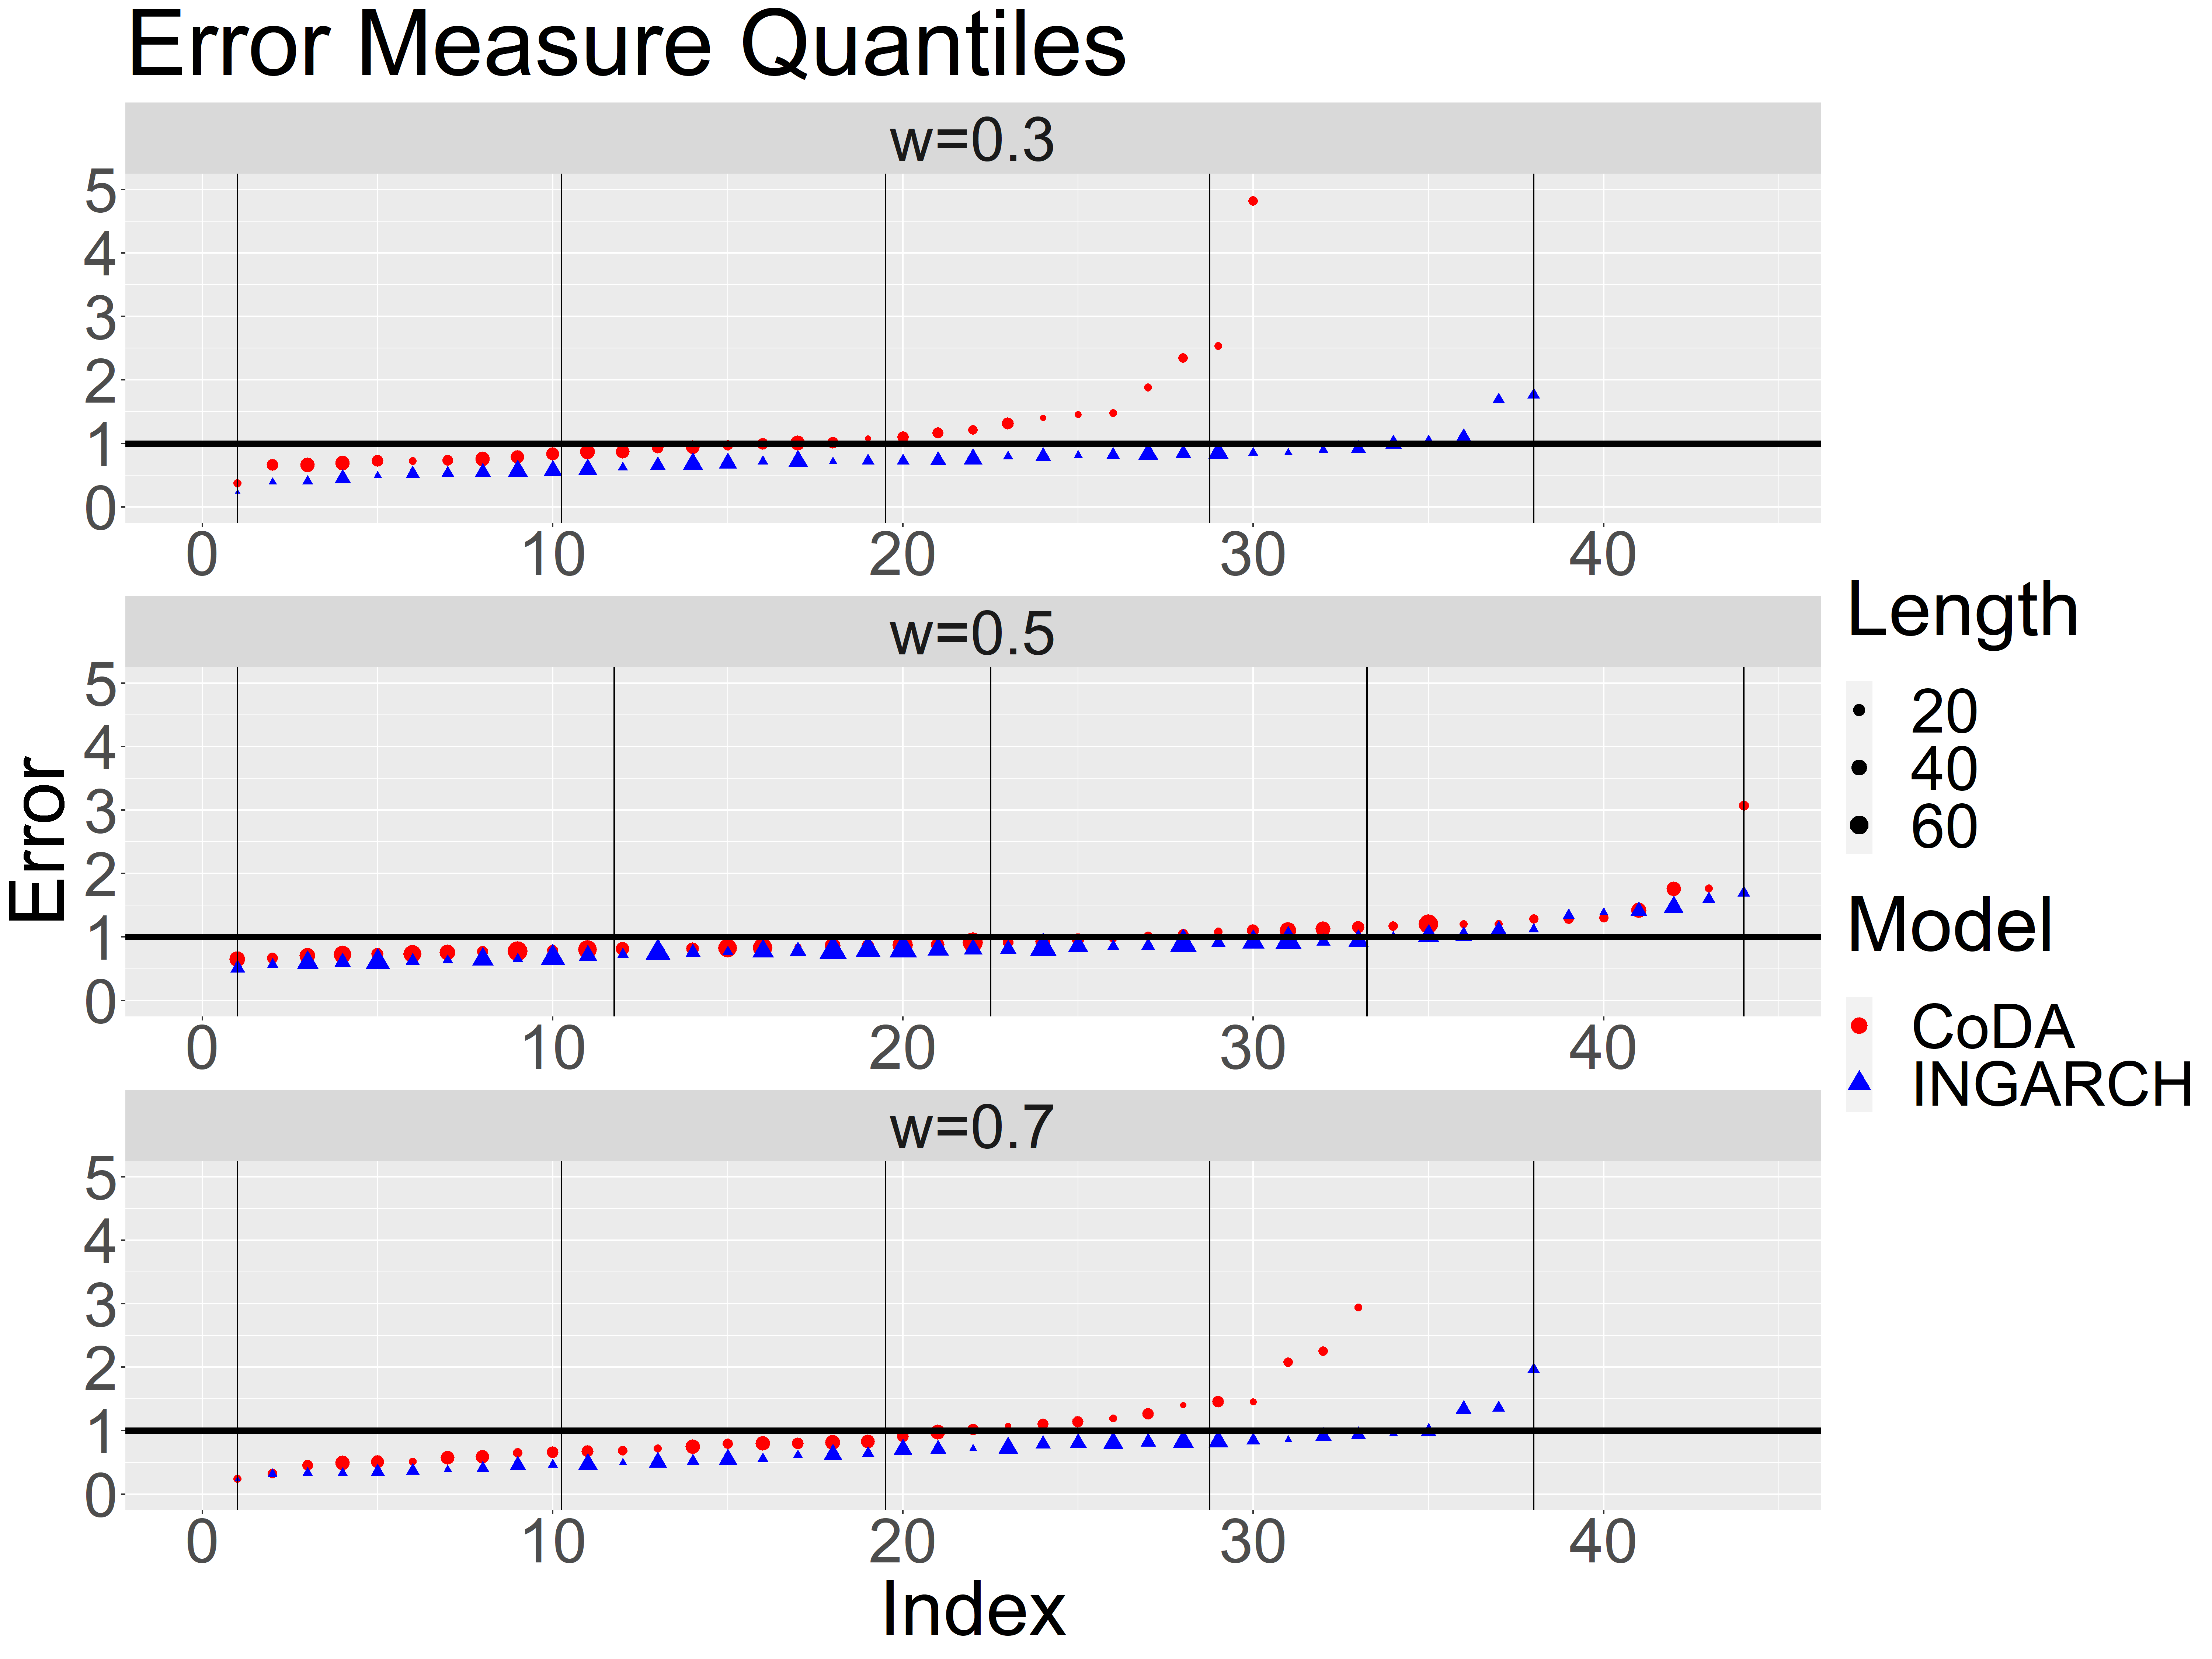
\includegraphics[width=\textwidth]{ErrorMeasureCombined_Quant_all__Variation_frame.png}
\caption{Quantiles of different $w$}
\label{fig:Frame Quant}
\end{subfigure}
\caption{Comparison of different $w$}
\label{fig:Frame Comp1}
\end{figure}


In the boxplot \ref{fig:Frame Box} it looks like INGARCH performs worst for $w=0.5$. However, in the quantile plot \ref{fig:Frame Quant} we can see that for $w=0.3,0.7$ the last errors are not included  in the plot. This could either be a result of them being to high, or that the model couldn't be fit on those fridges. 

For CoDA there seems not to be much difference. The best results are obtained with $w=0.3$, but the differences are only marginal. 


\subsubsection{Window Shape}
\label{sec:Window Shape}

We also vary the shape of the window. As explained in \ref{sec: Model Specification} we either use a fixed amount of points and add and remove points as time goes on, or we continuously add points to the window. The results are in figures \ref{fig:window methods Comp1}. We can see that there are no big differences between the methods. For both, CoDA and INGARCH, there are no notable difference. 

\begin{figure}[htb!]
\centering
\begin{subfigure}[b]{0.45\textwidth}
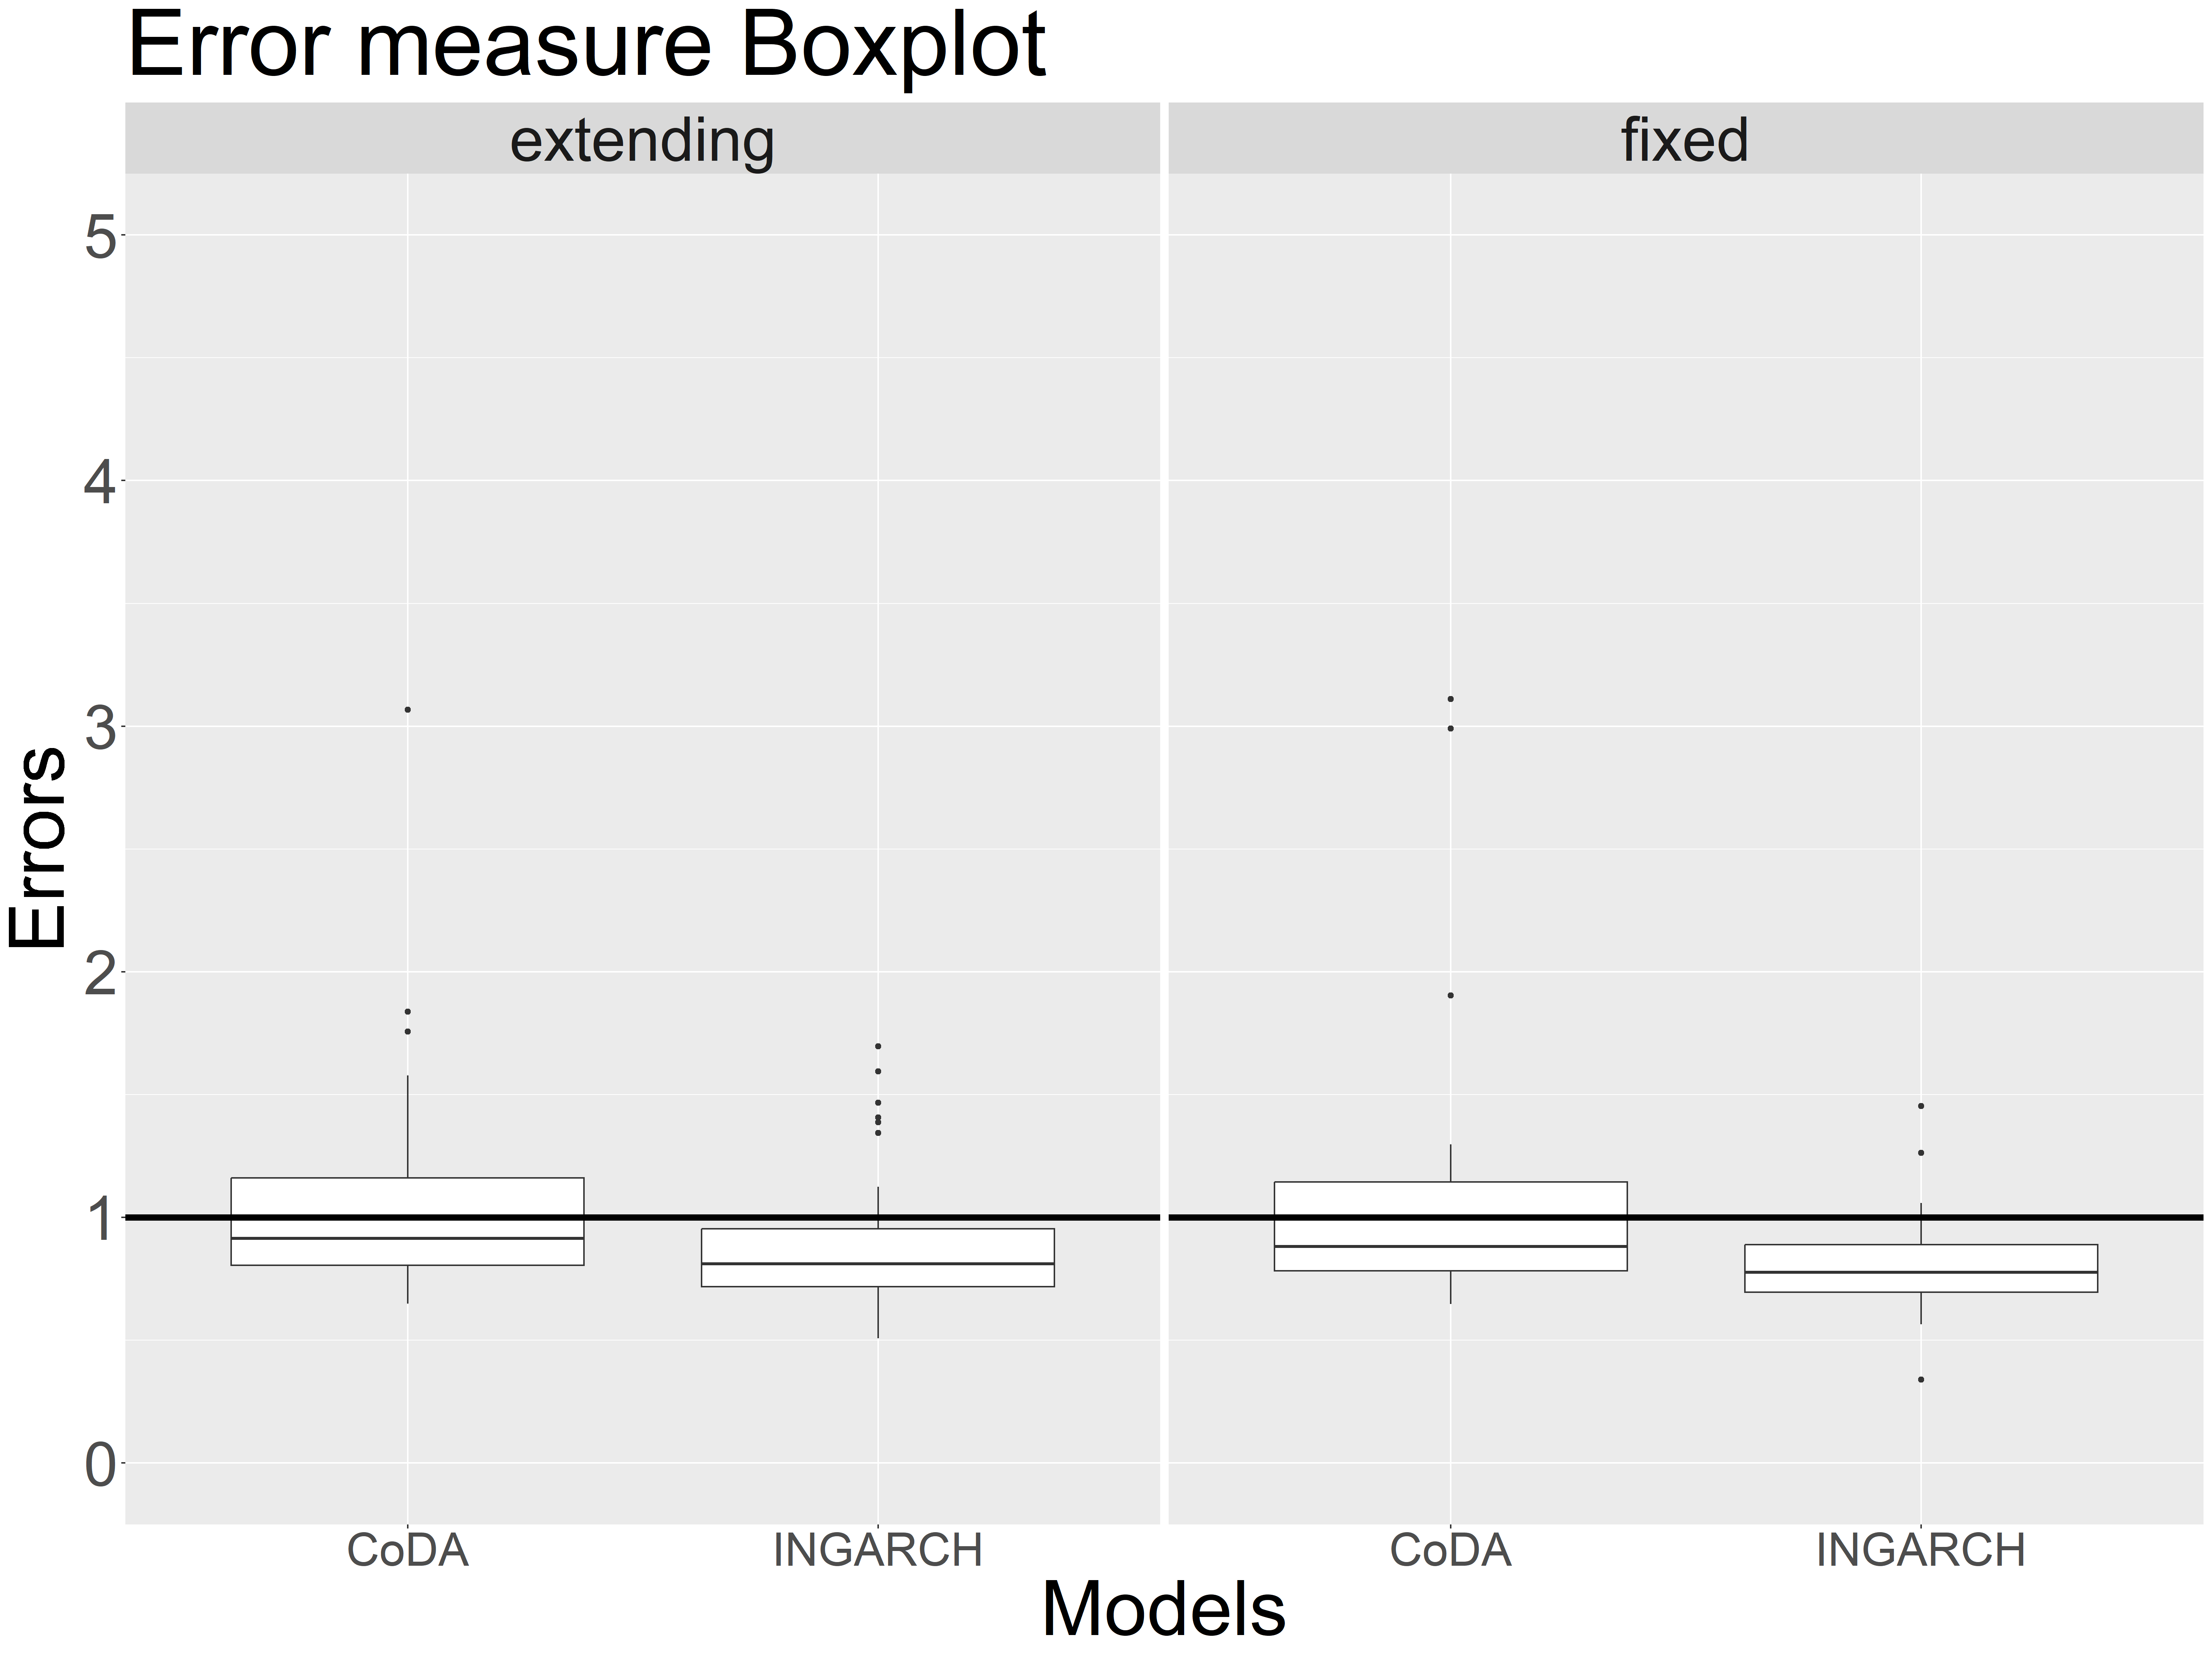
\includegraphics[width=\textwidth]{ErrorMeasureCombined_Box_all__Variation_windowMethod.png}
\caption{Boxplot for different window shapes}
\label{fig:window methods Box}
\end{subfigure}
\hfill
\begin{subfigure}[b]{0.45\textwidth}
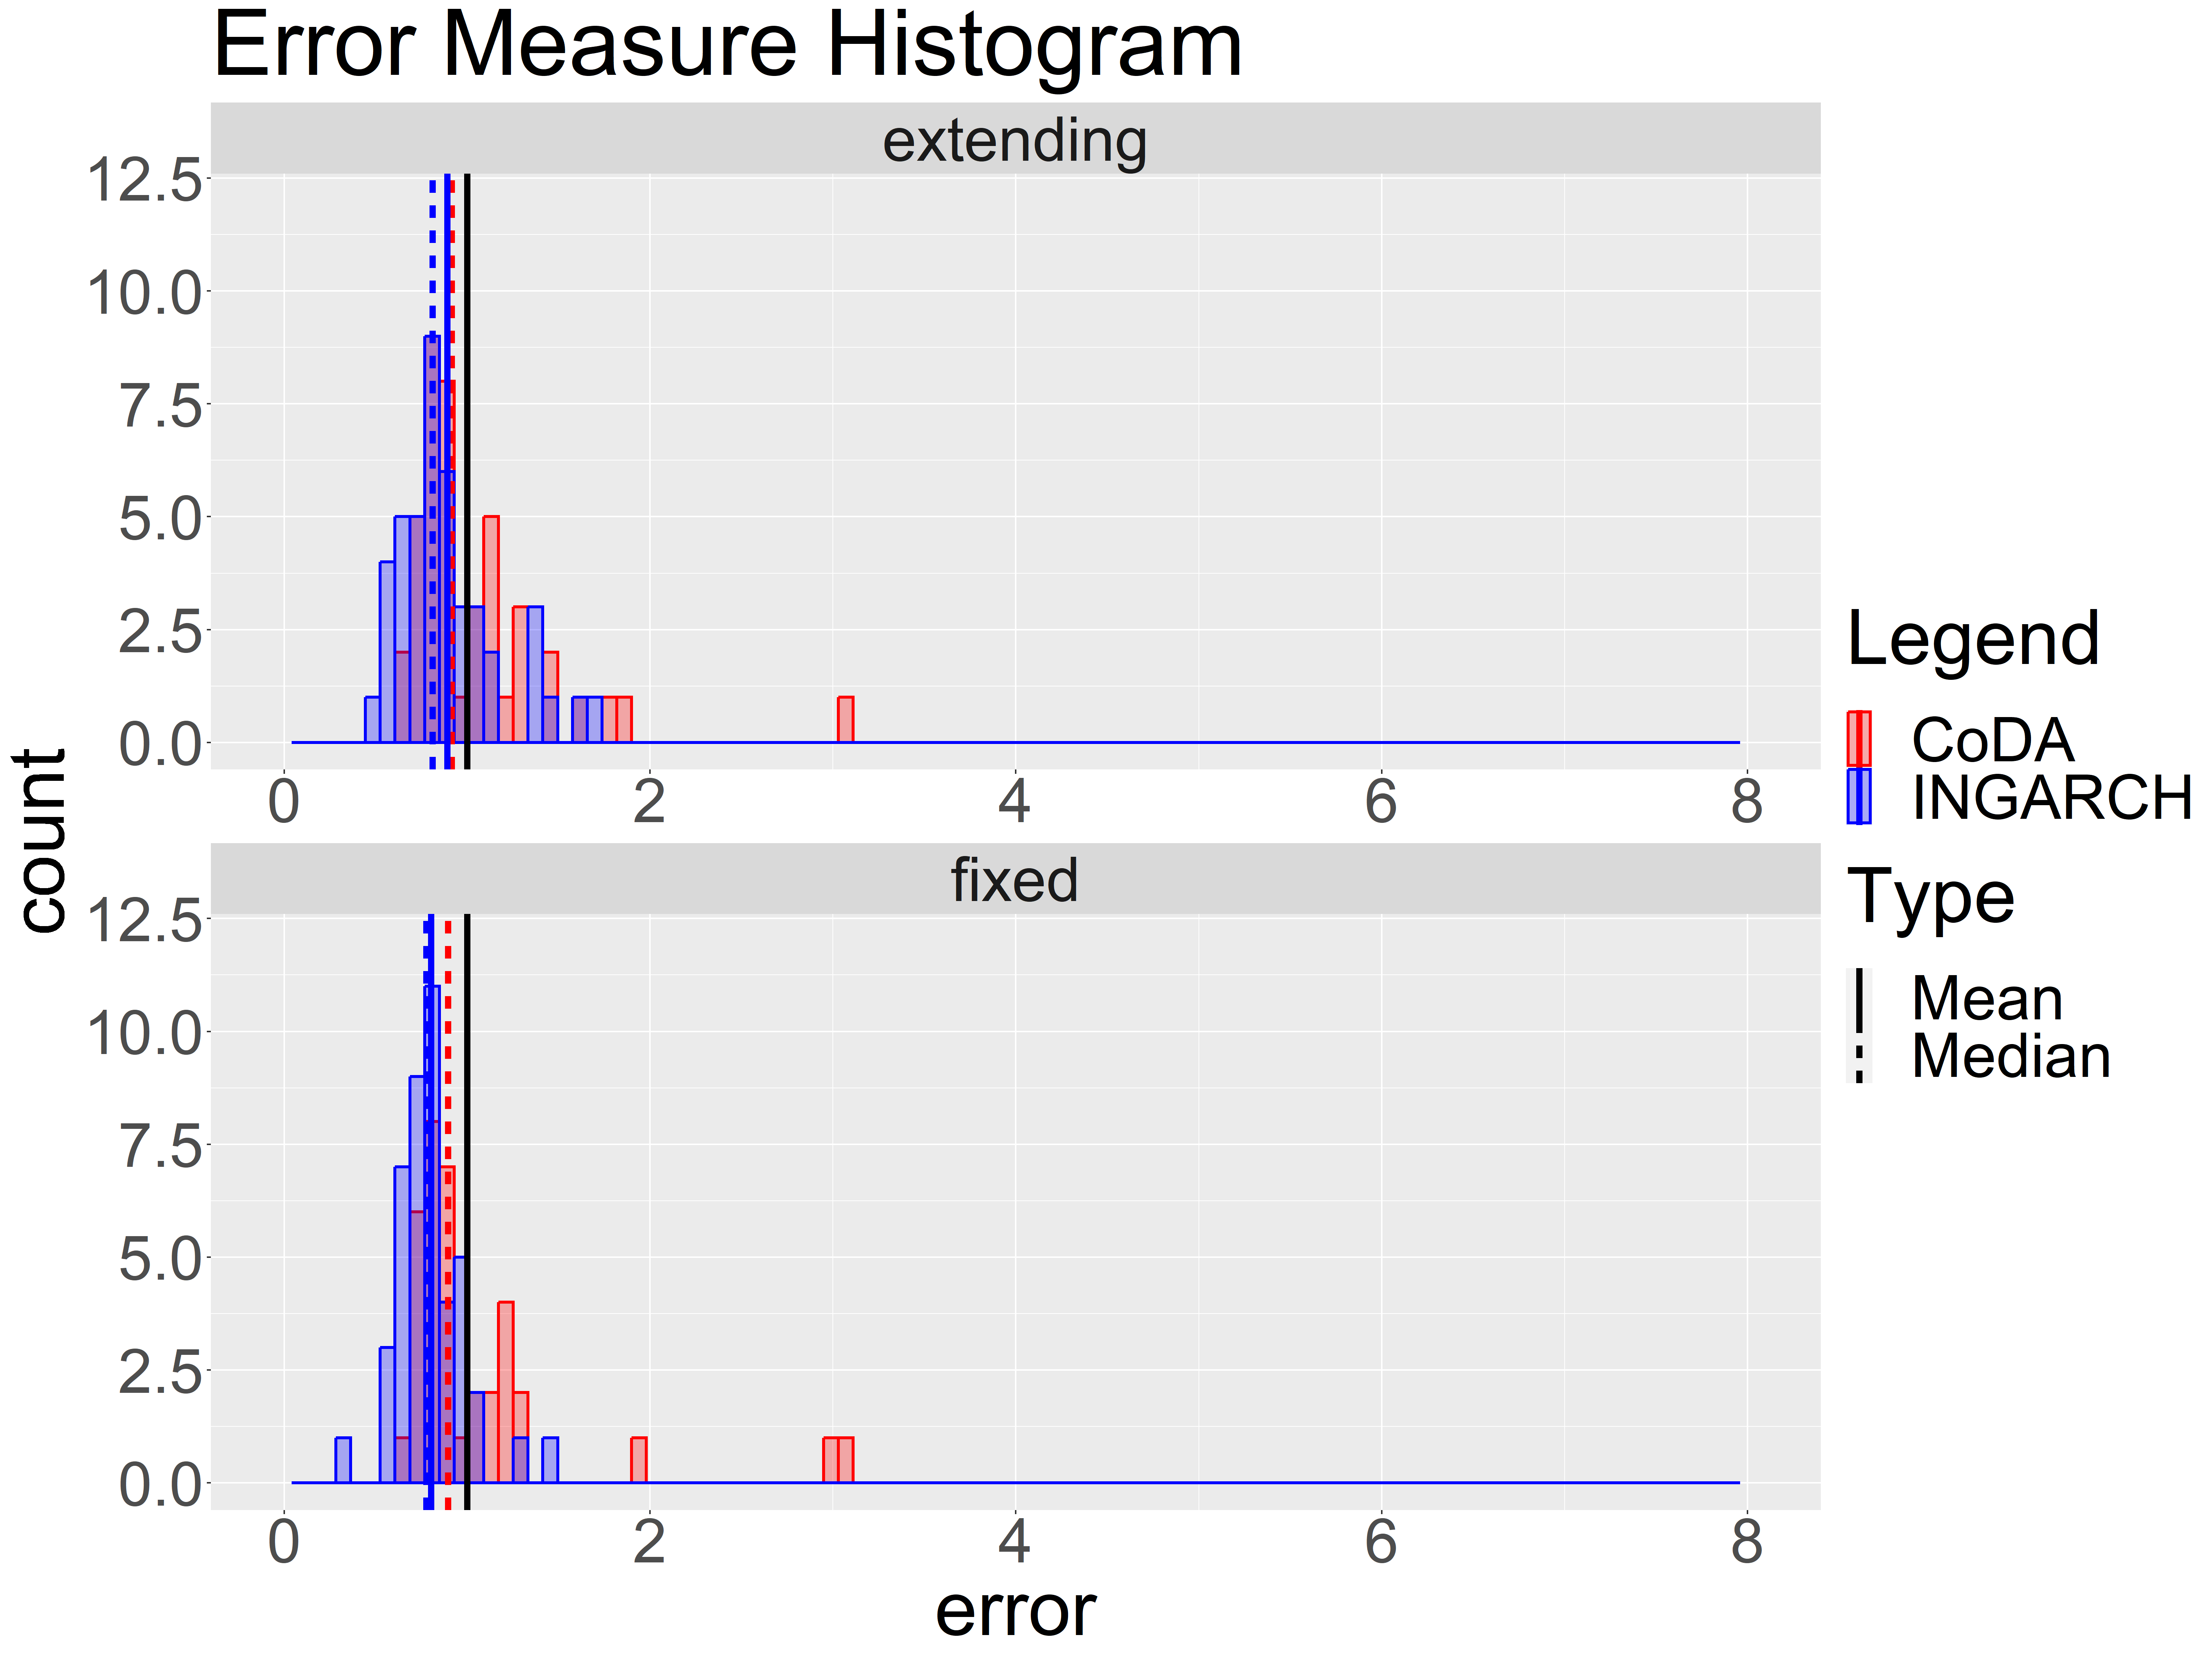
\includegraphics[width=\textwidth]{ErrorMeasureCombined_Histogram_all__Variation_windowMethod.png}
\caption{Histogram for different window shapes}
\label{fig:window methods Hist}
\end{subfigure}
\hfill
\begin{subfigure}[b]{0.8\textwidth}
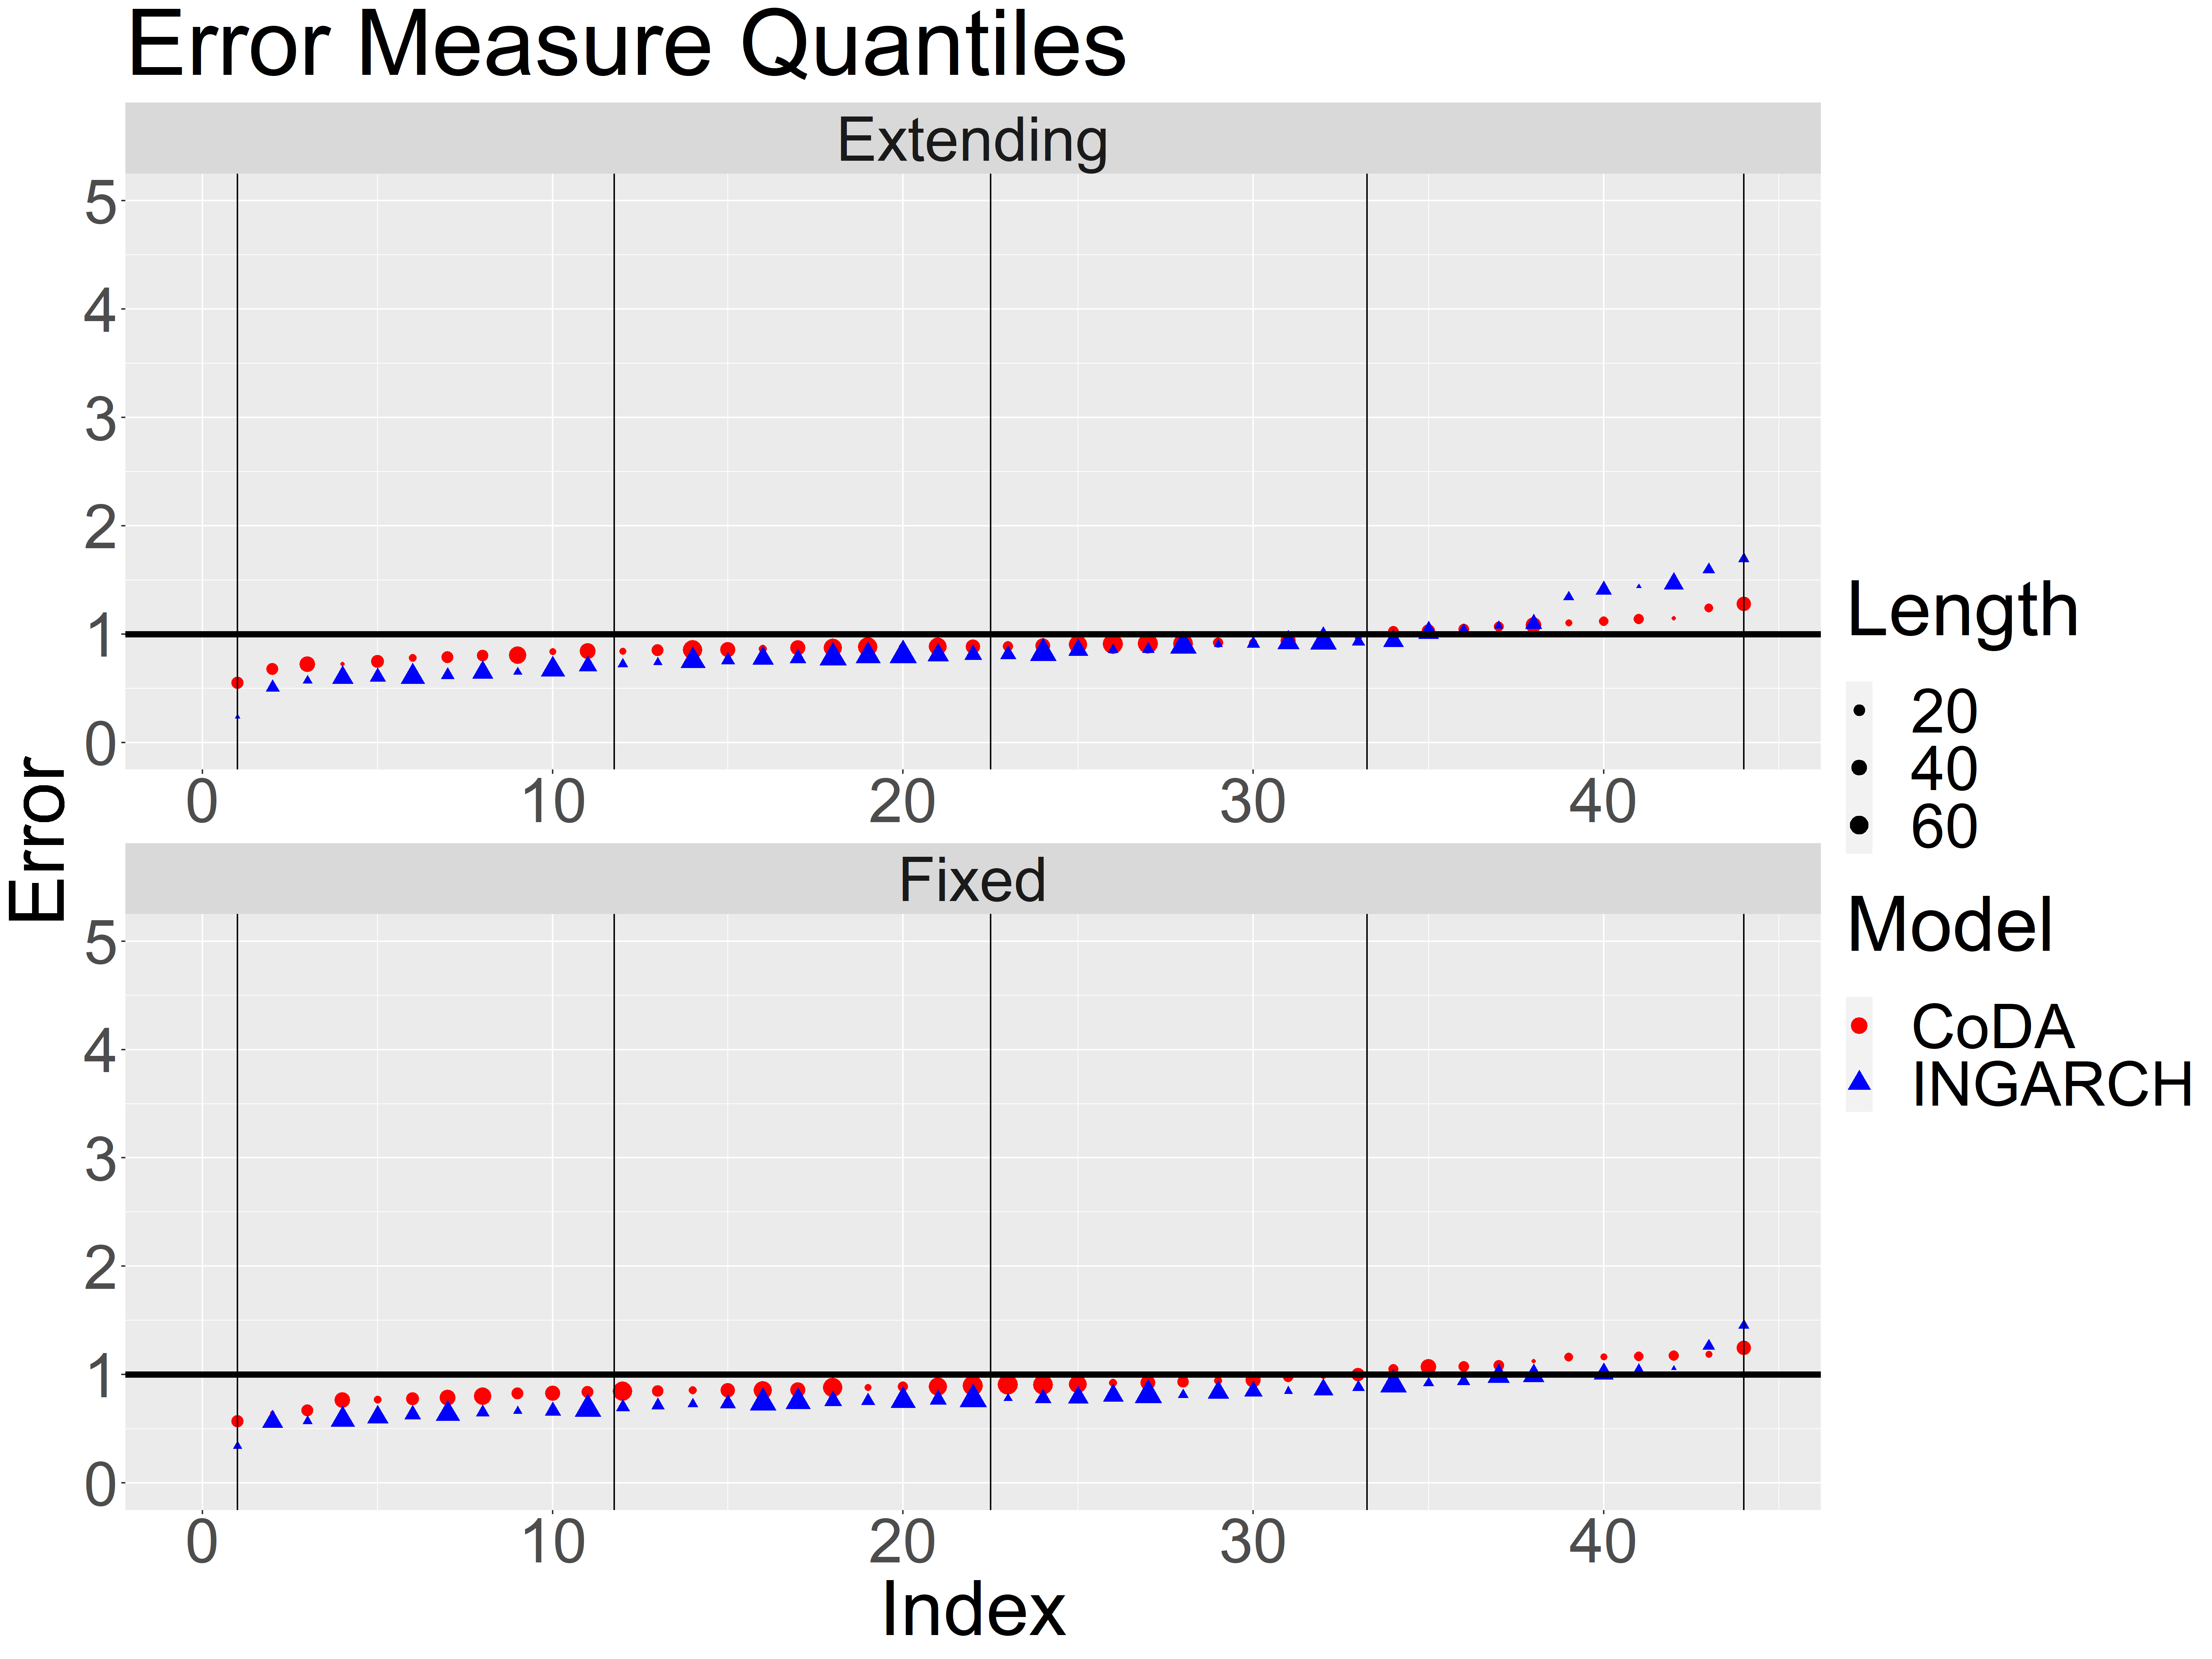
\includegraphics[width=\textwidth]{ErrorMeasureCombined_Quant_all__Variation_windowMethod.png}
\caption{Quantiles for different window shapes}
\label{fig:window methods Quant}
\end{subfigure}
\caption{Comparison of different window shapes}
\label{fig:window methods Comp1}
\end{figure}


\subsection{INGARCH Specifications Results}
\label{sec: Ingarch Specifications Results}

Next we will investigate the INGARCH specific options. As before, we use the standard settings for the INGARCH(1,1) model and always vary one parameter. 

\subsubsection{Distribution}
\label{sec:Distribution}

As mentioned in \ref{sec: Ingarch Specifications} we can replace the Poisson distribution with a Negative Binomial Distribution in \ref{eq:Ingarch Distribution}. The results are shown in \ref{fig:distributions Comp1}. 

\begin{figure}[htb!]
\centering
\begin{subfigure}[b]{0.45\textwidth}
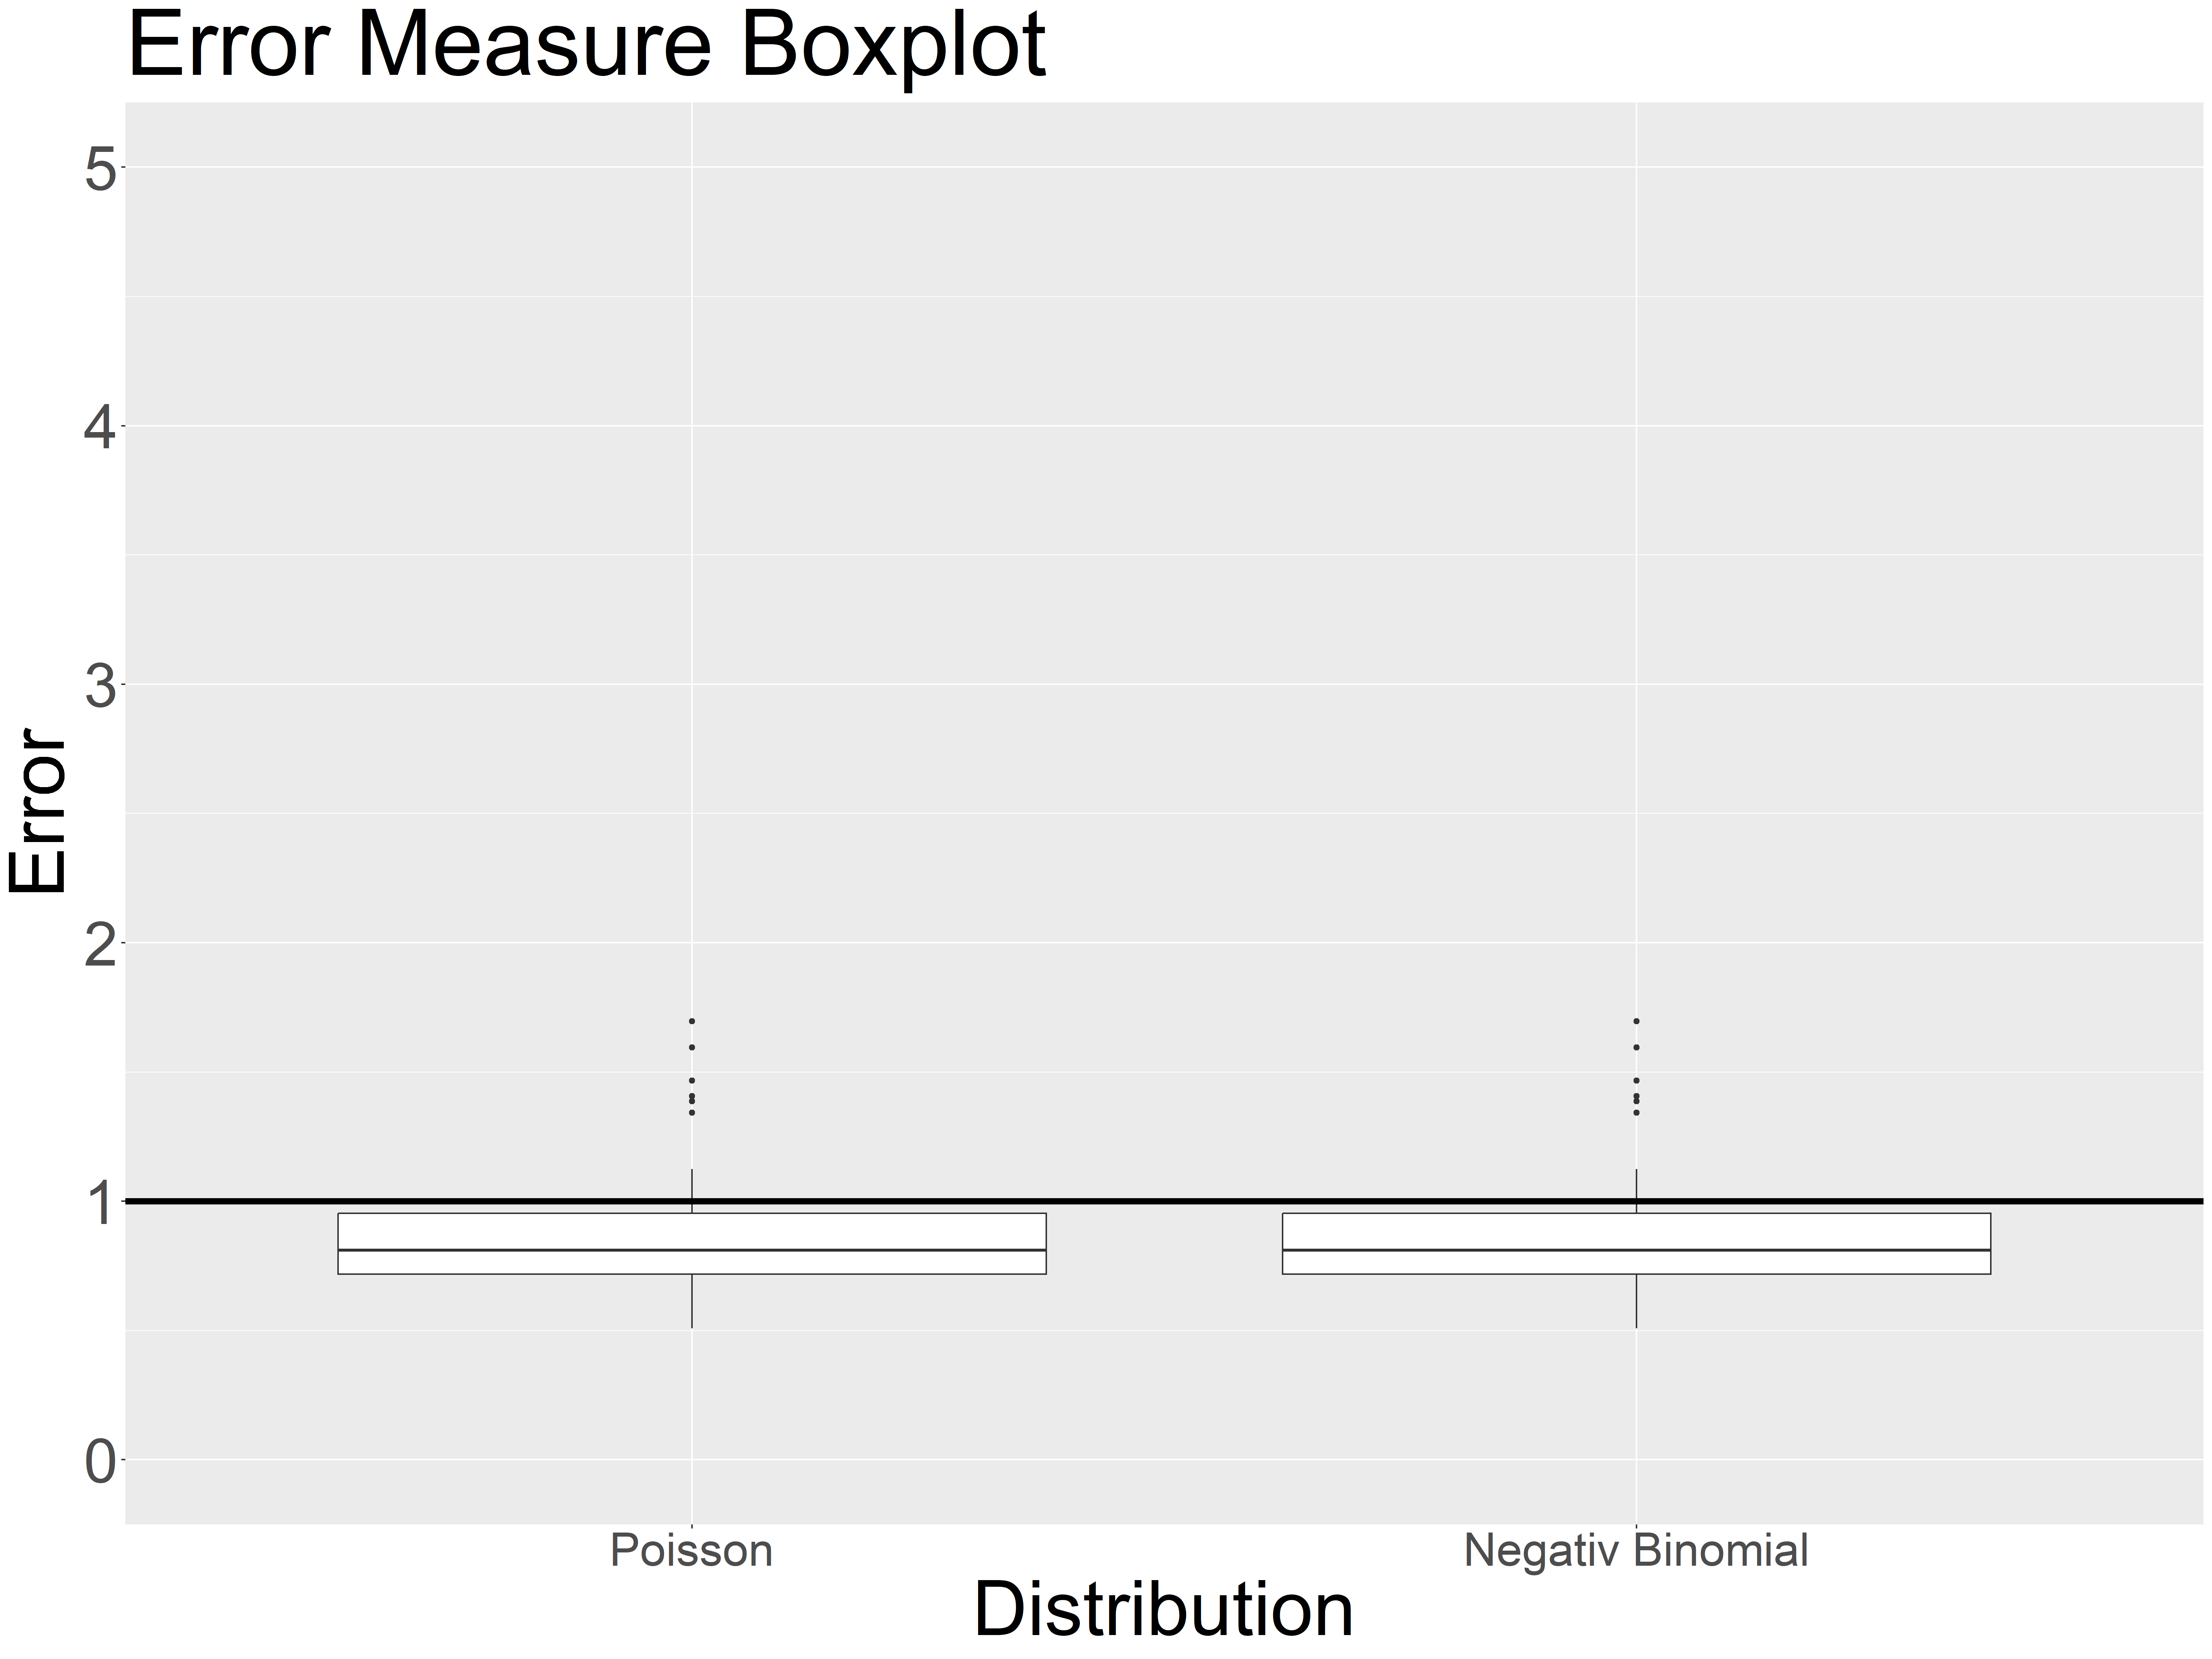
\includegraphics[width=\textwidth]{ErrorMeasureINGARCH_Box_all__Variation_distribution.png}
\caption{Boxplot for different distributions}
\label{fig:distributions Box}
\end{subfigure}
\hfill
\begin{subfigure}[b]{0.45\textwidth}
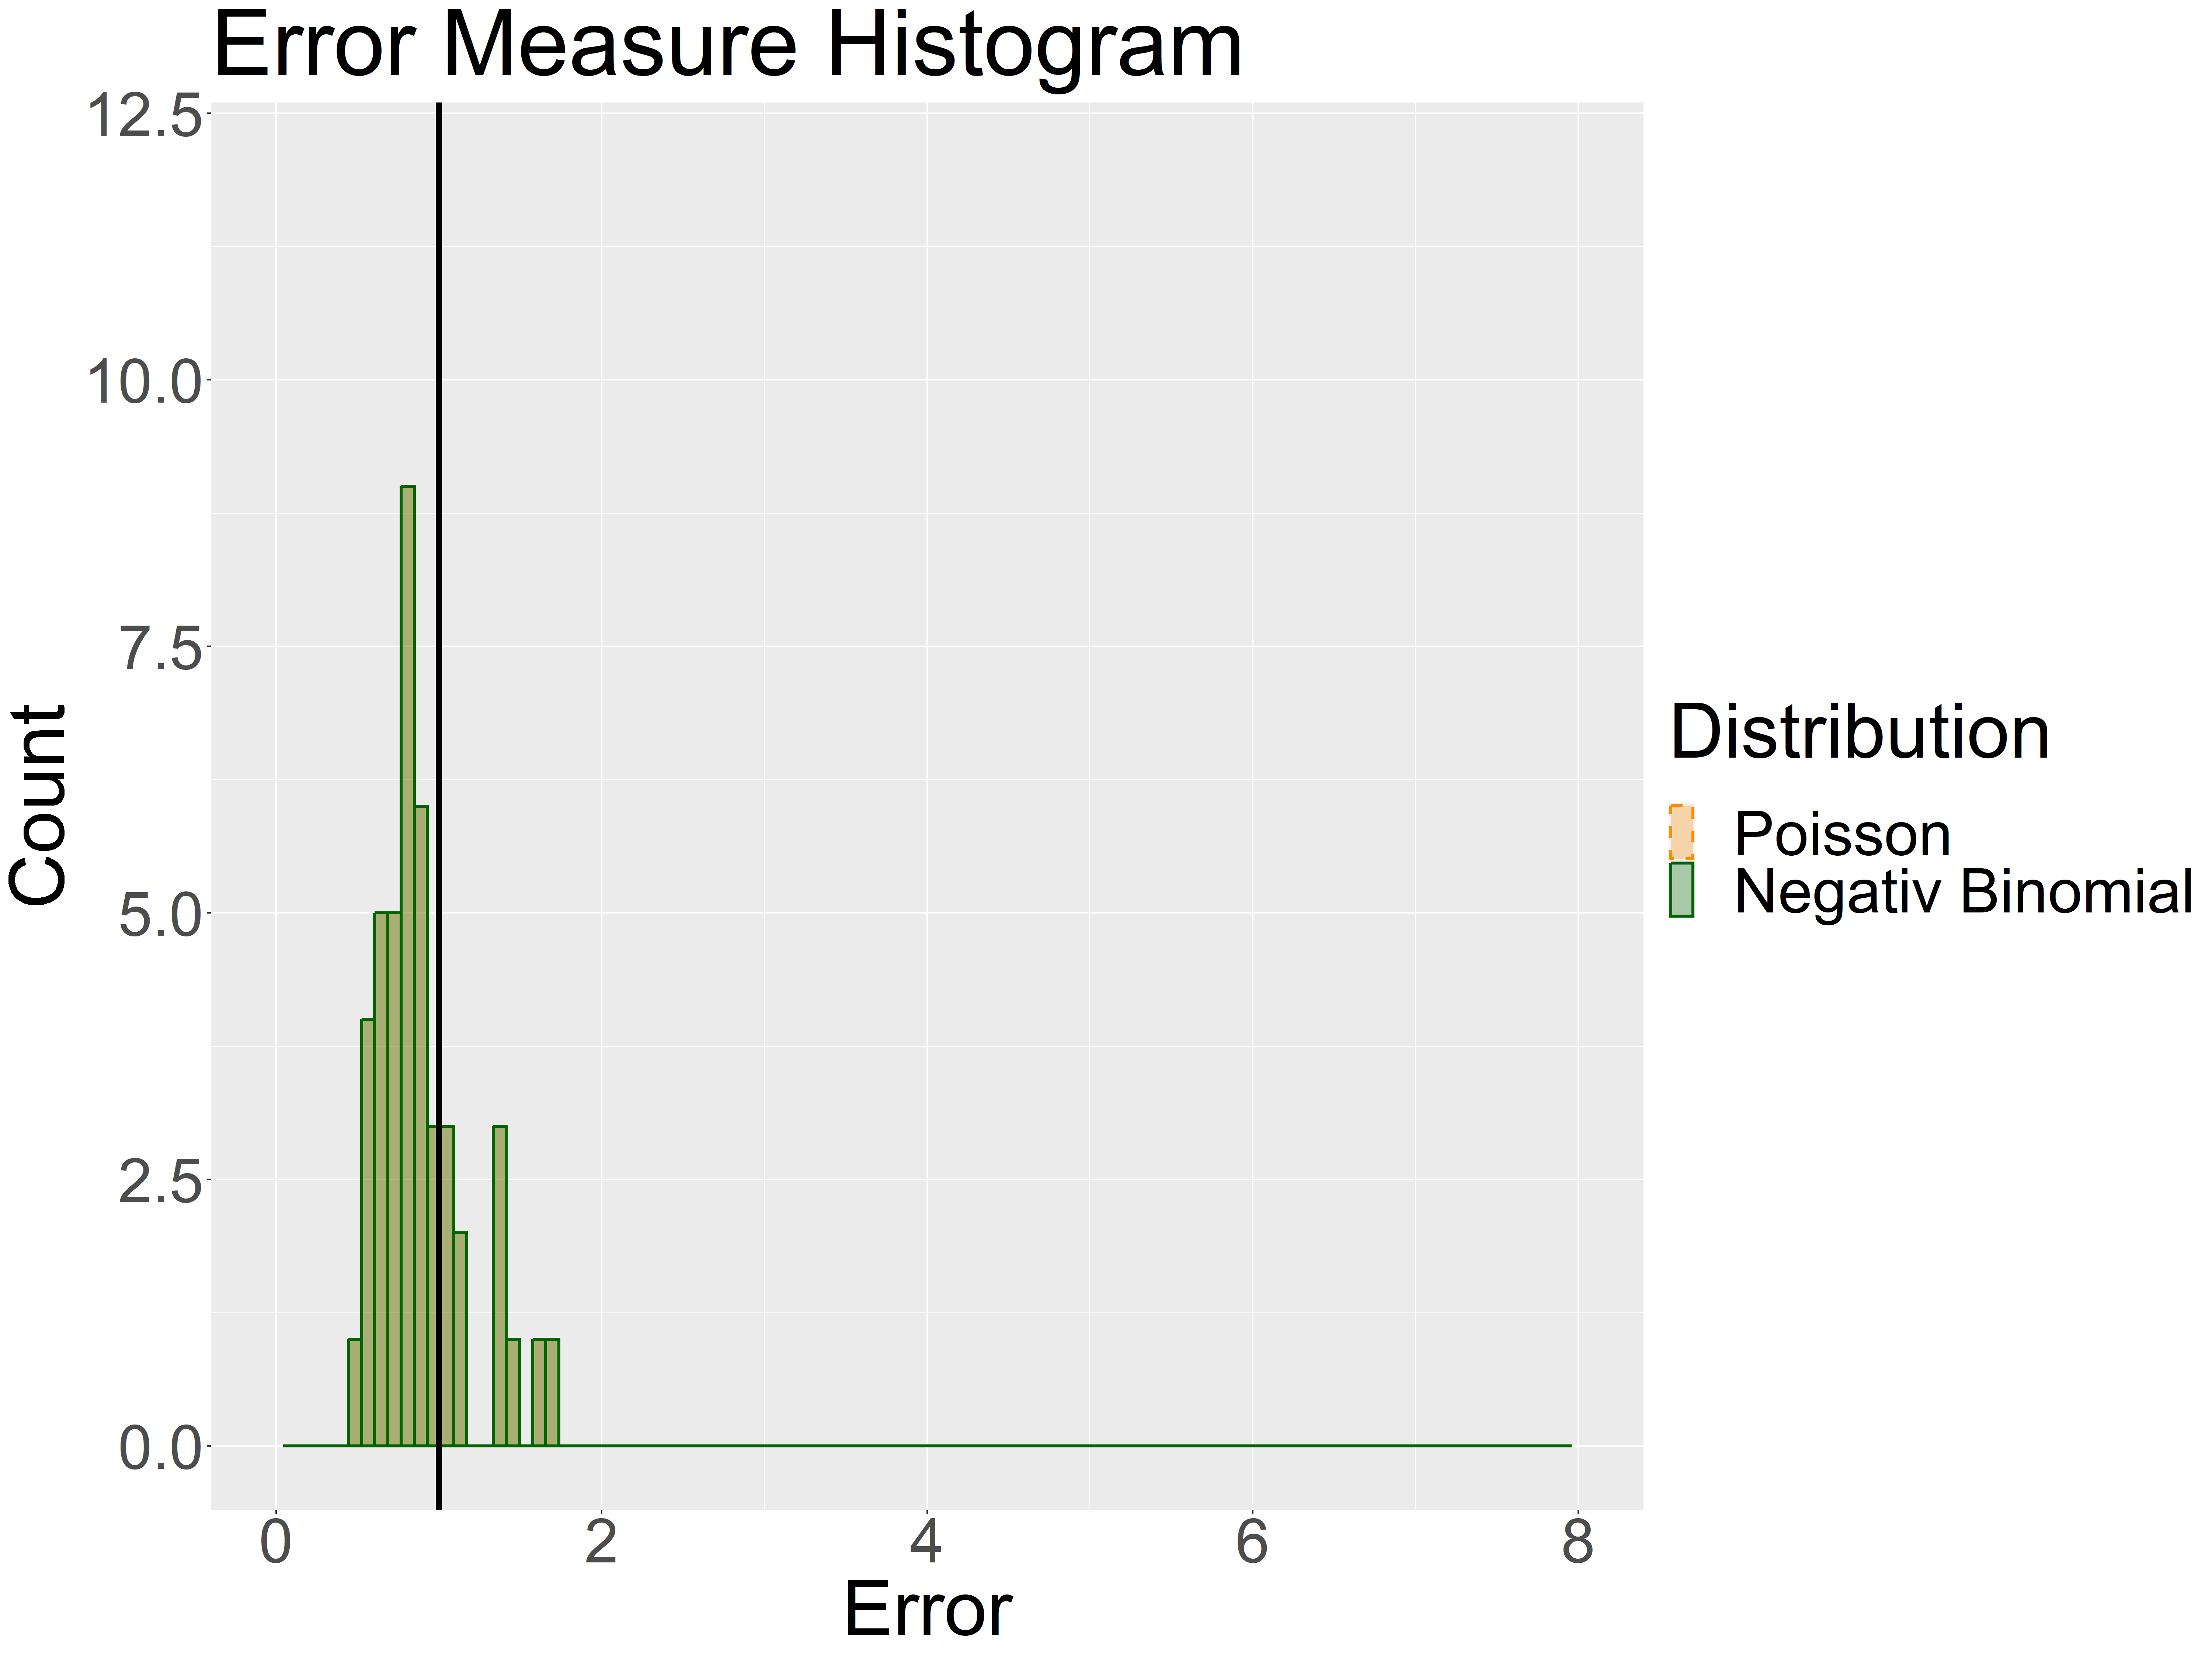
\includegraphics[width=\textwidth]{ErrorMeasureINGARCH_Histogram_all__Variation_distribution.png}
\caption{Histogram for different distributions}
\label{fig:distributions Hist}
\end{subfigure}
\hfill
%\begin{subfigure}[b]{0.8\textwidth}
%\includegraphics[width=\textwidth]{ErrorMeasureINGARCH_Quant_all__Variation_windowMethod.png}
%\caption{Quantiles for different distributions}
%\label{fig:window methods Quant}
%\end{subfigure}
\caption{Comparison of different distributions}
\label{fig:distributions Comp1}
\end{figure}

As we can see, we get the exactly the same results for both distributions. However, as mentioned in \ref{sec: Estimation of the Ingarch Model}, we round the predicted conditional mean to the next integer. Hence, we could get slightly different results for the different distributions. Nevertheless, the difference is still negligible. %Since the Poisson Distribution is a limiting case of the Negative Binomial Distribution when $\phi \longrightarrow \infty$ in \ref{eq:Ingarch negbinom Distribution}, \cite{Liboschik:2016}. 


\subsubsection{Number of Past Means and Observations}
\label{sec: Number of Past Means and Observations}

The order in the INGARCH(p,q) model is another parameter which can be chosen. For simplicities sake we only compare our INGARCH(1,1) with an INGARCH(1,2) and INGARCH(2,1) model. However, further models could be tried out and compared. 

In figure \ref{fig:past means Comp1} we compare the INGARCH(1,1) model (red) with the INGARCH(1,2) model (blue). We can see that the performance is very similar. Hence we prefer the smaller model. 
\begin{figure}[htb!]
\centering
\begin{subfigure}[b]{0.45\textwidth}
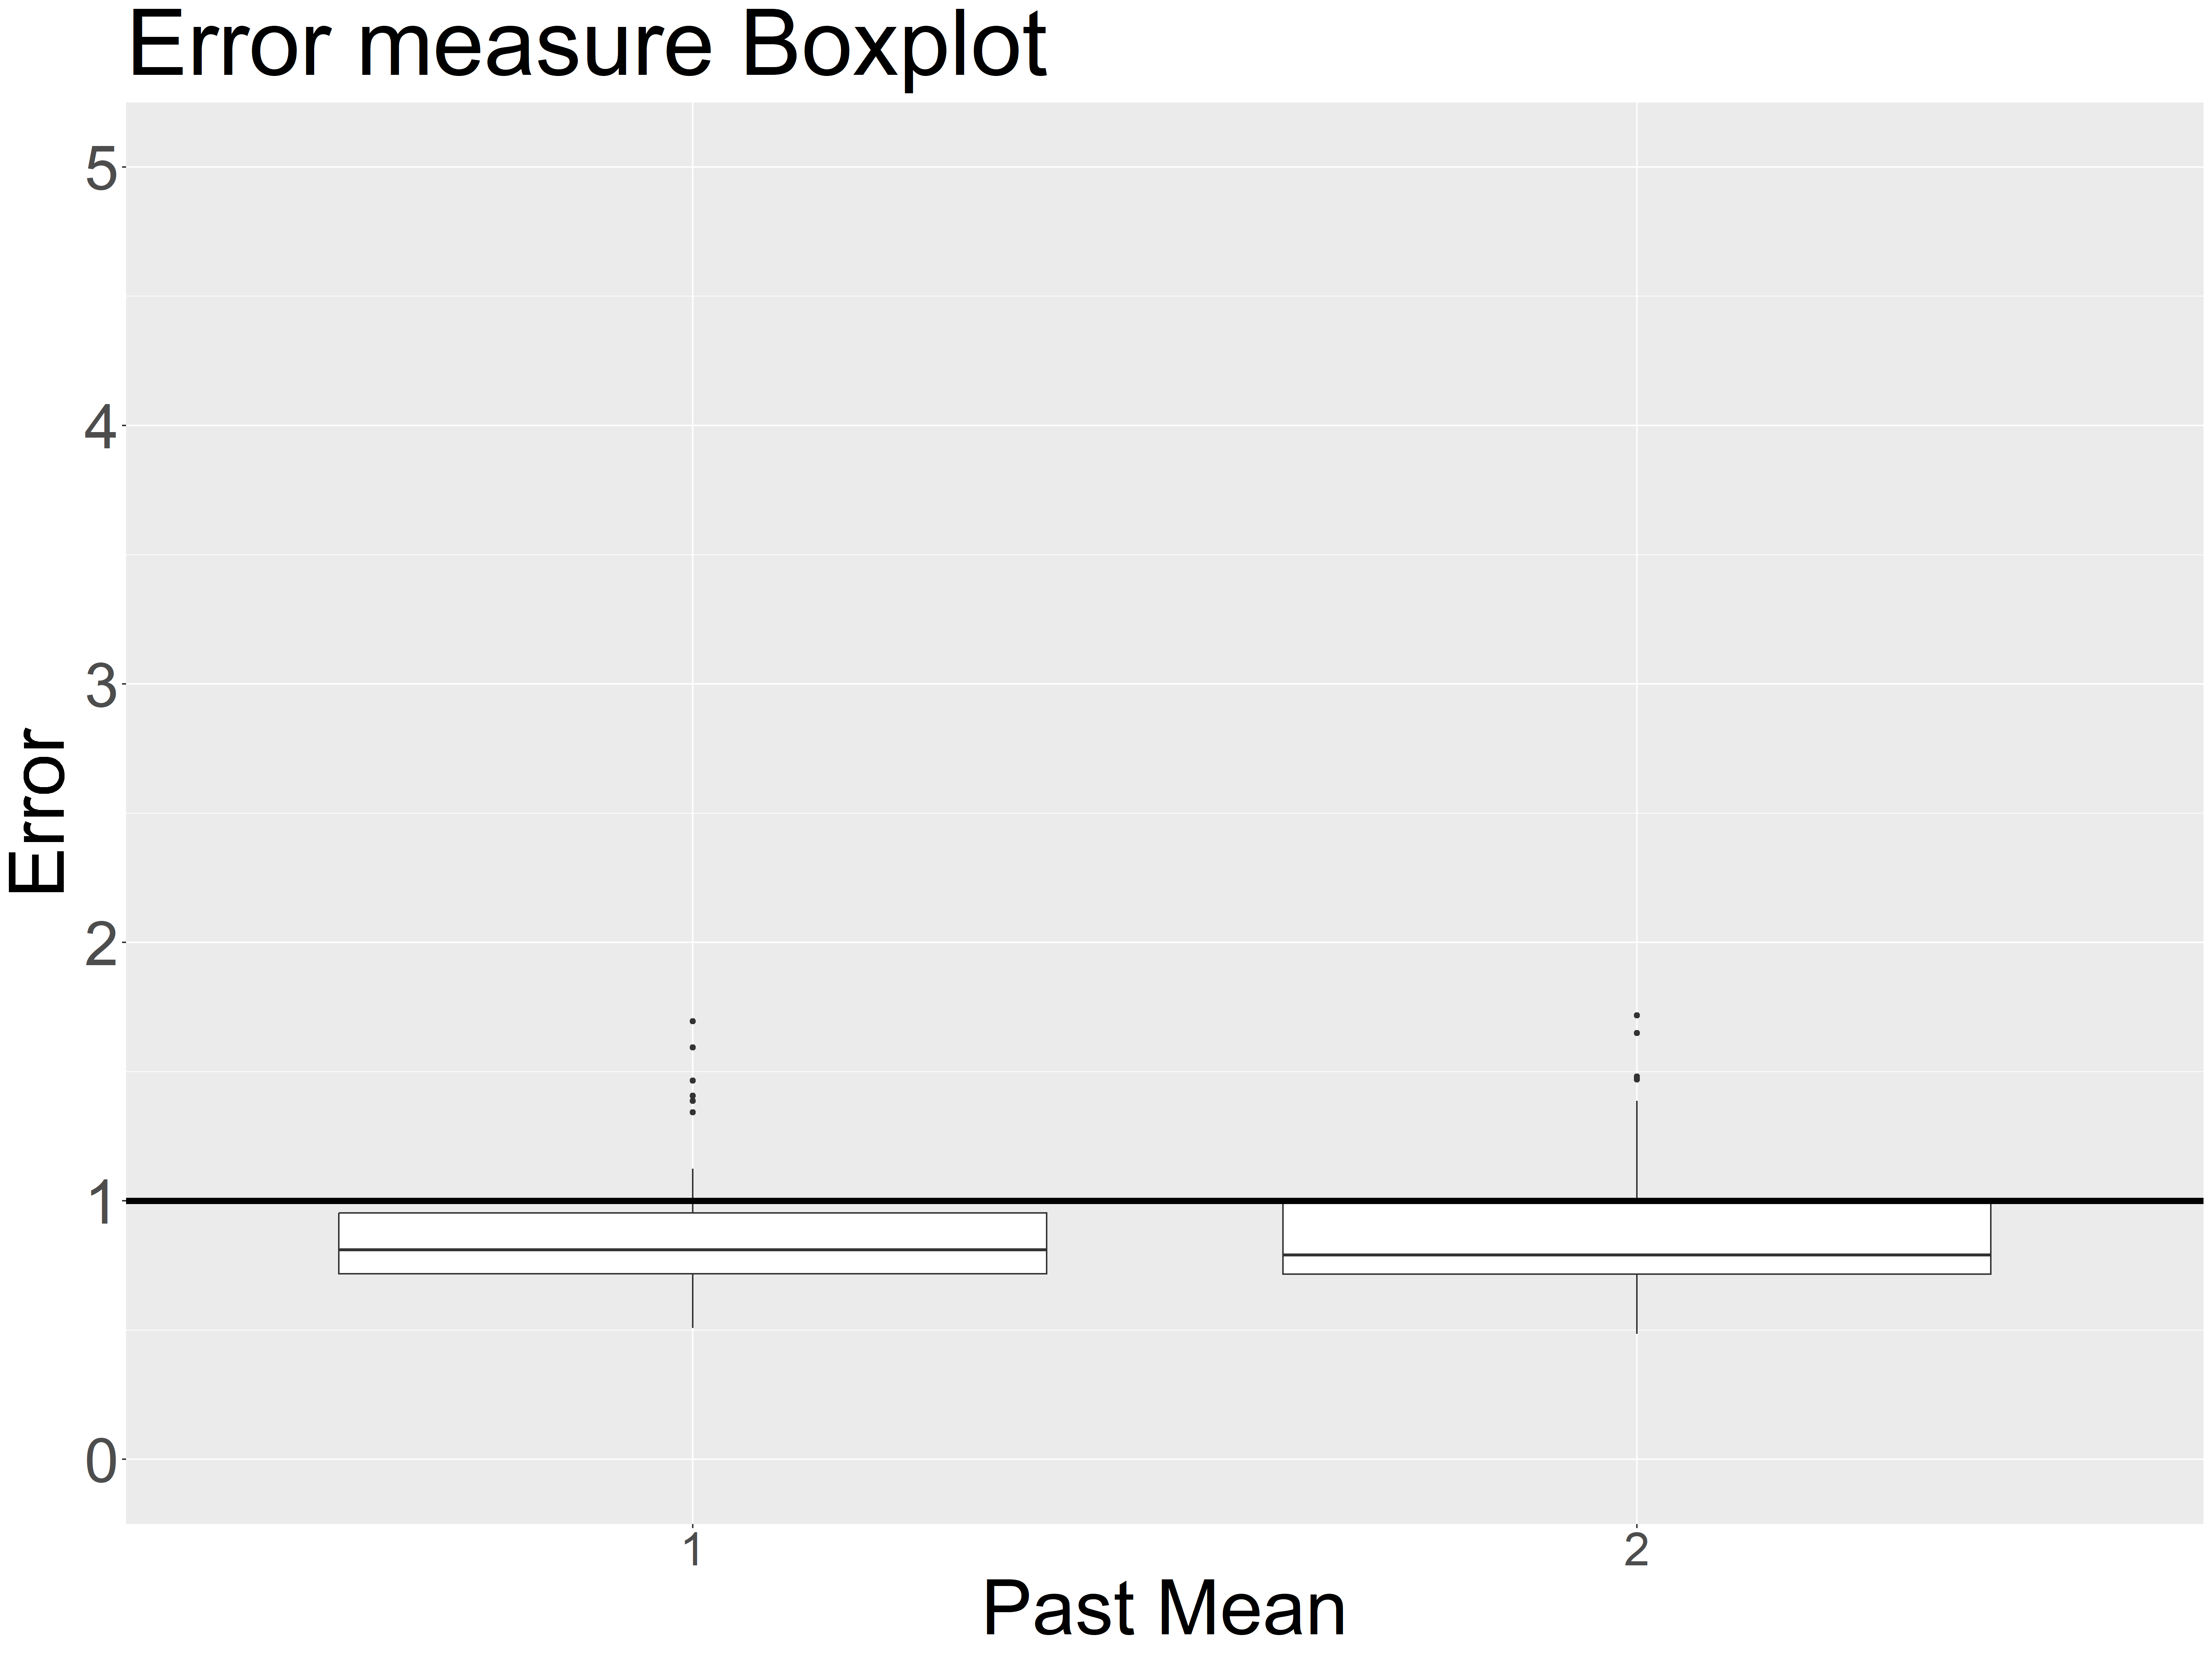
\includegraphics[width=\textwidth]{ErrorMeasureINGARCH_Box_all__Variation_pastMean.png}
\caption{Boxplot for a different number of past means}
\label{fig:past means Box}
\end{subfigure}
\hfill
\begin{subfigure}[b]{0.45\textwidth}
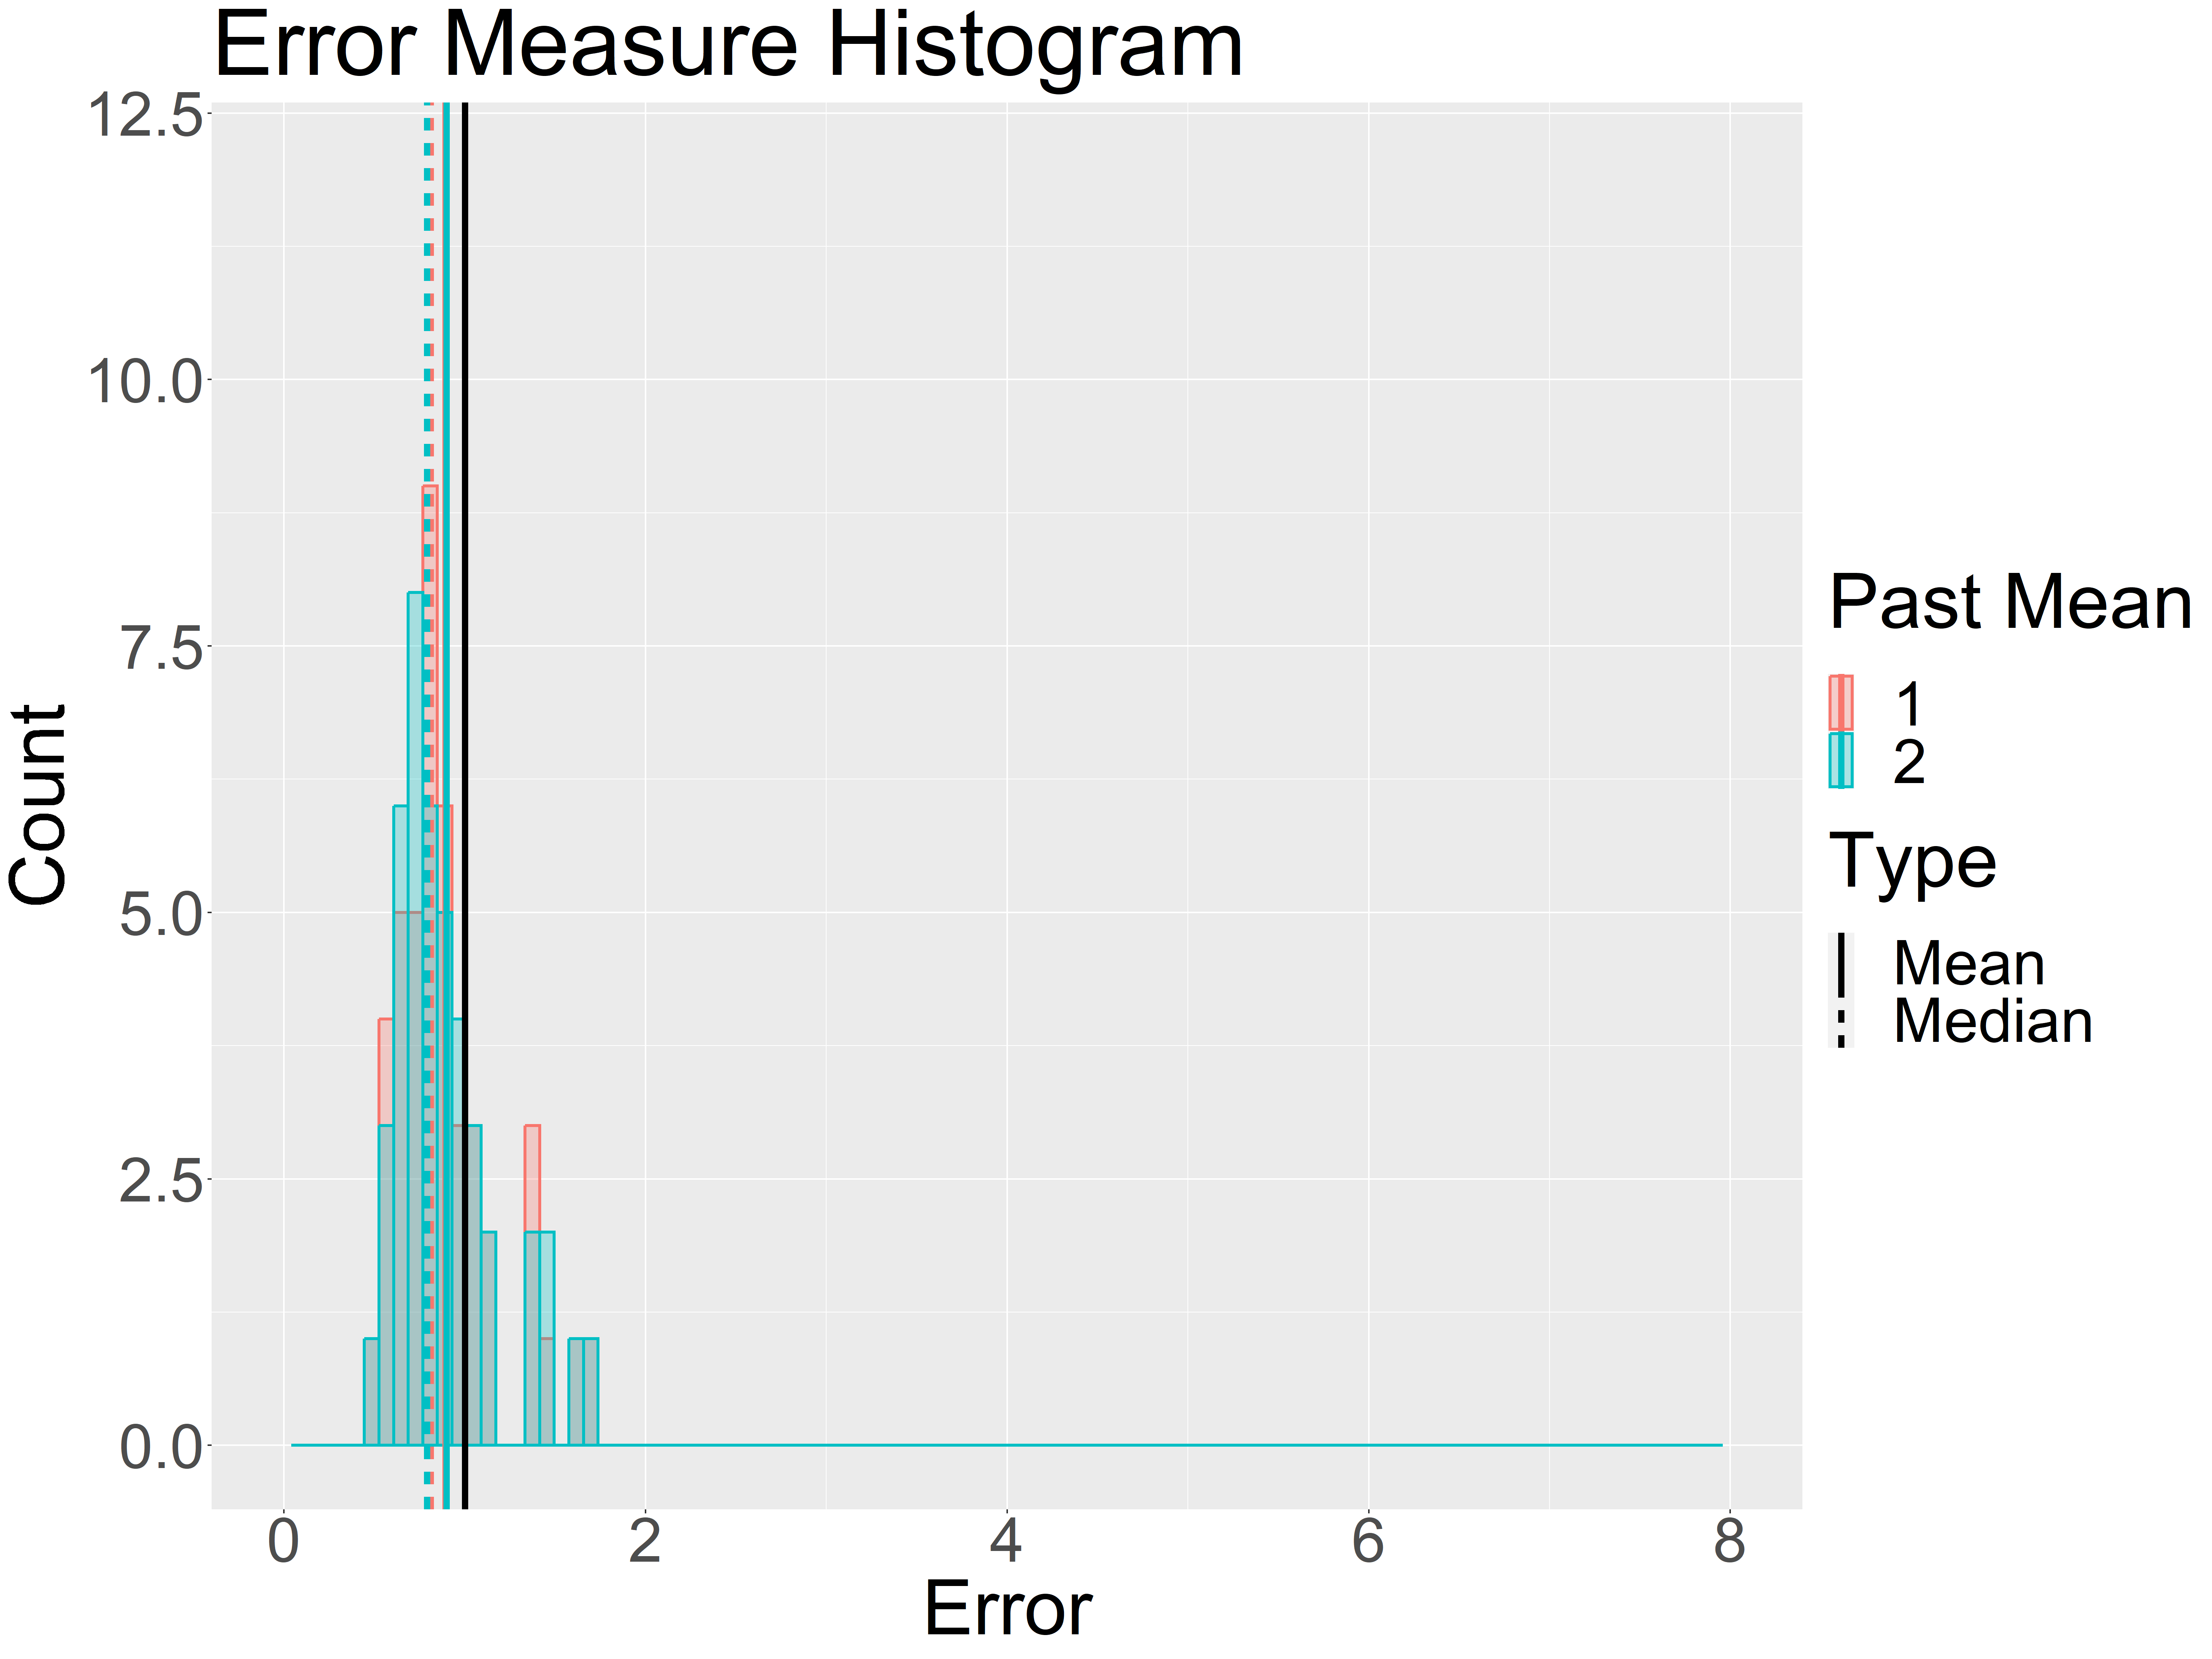
\includegraphics[width=\textwidth]{ErrorMeasureINGARCH_Histogram_all__Variation_pastMean.png}
\caption{Histogram for a different number of past means}
\label{fig:past means Hist}
\end{subfigure}
\hfill
\begin{subfigure}[b]{0.8\textwidth}
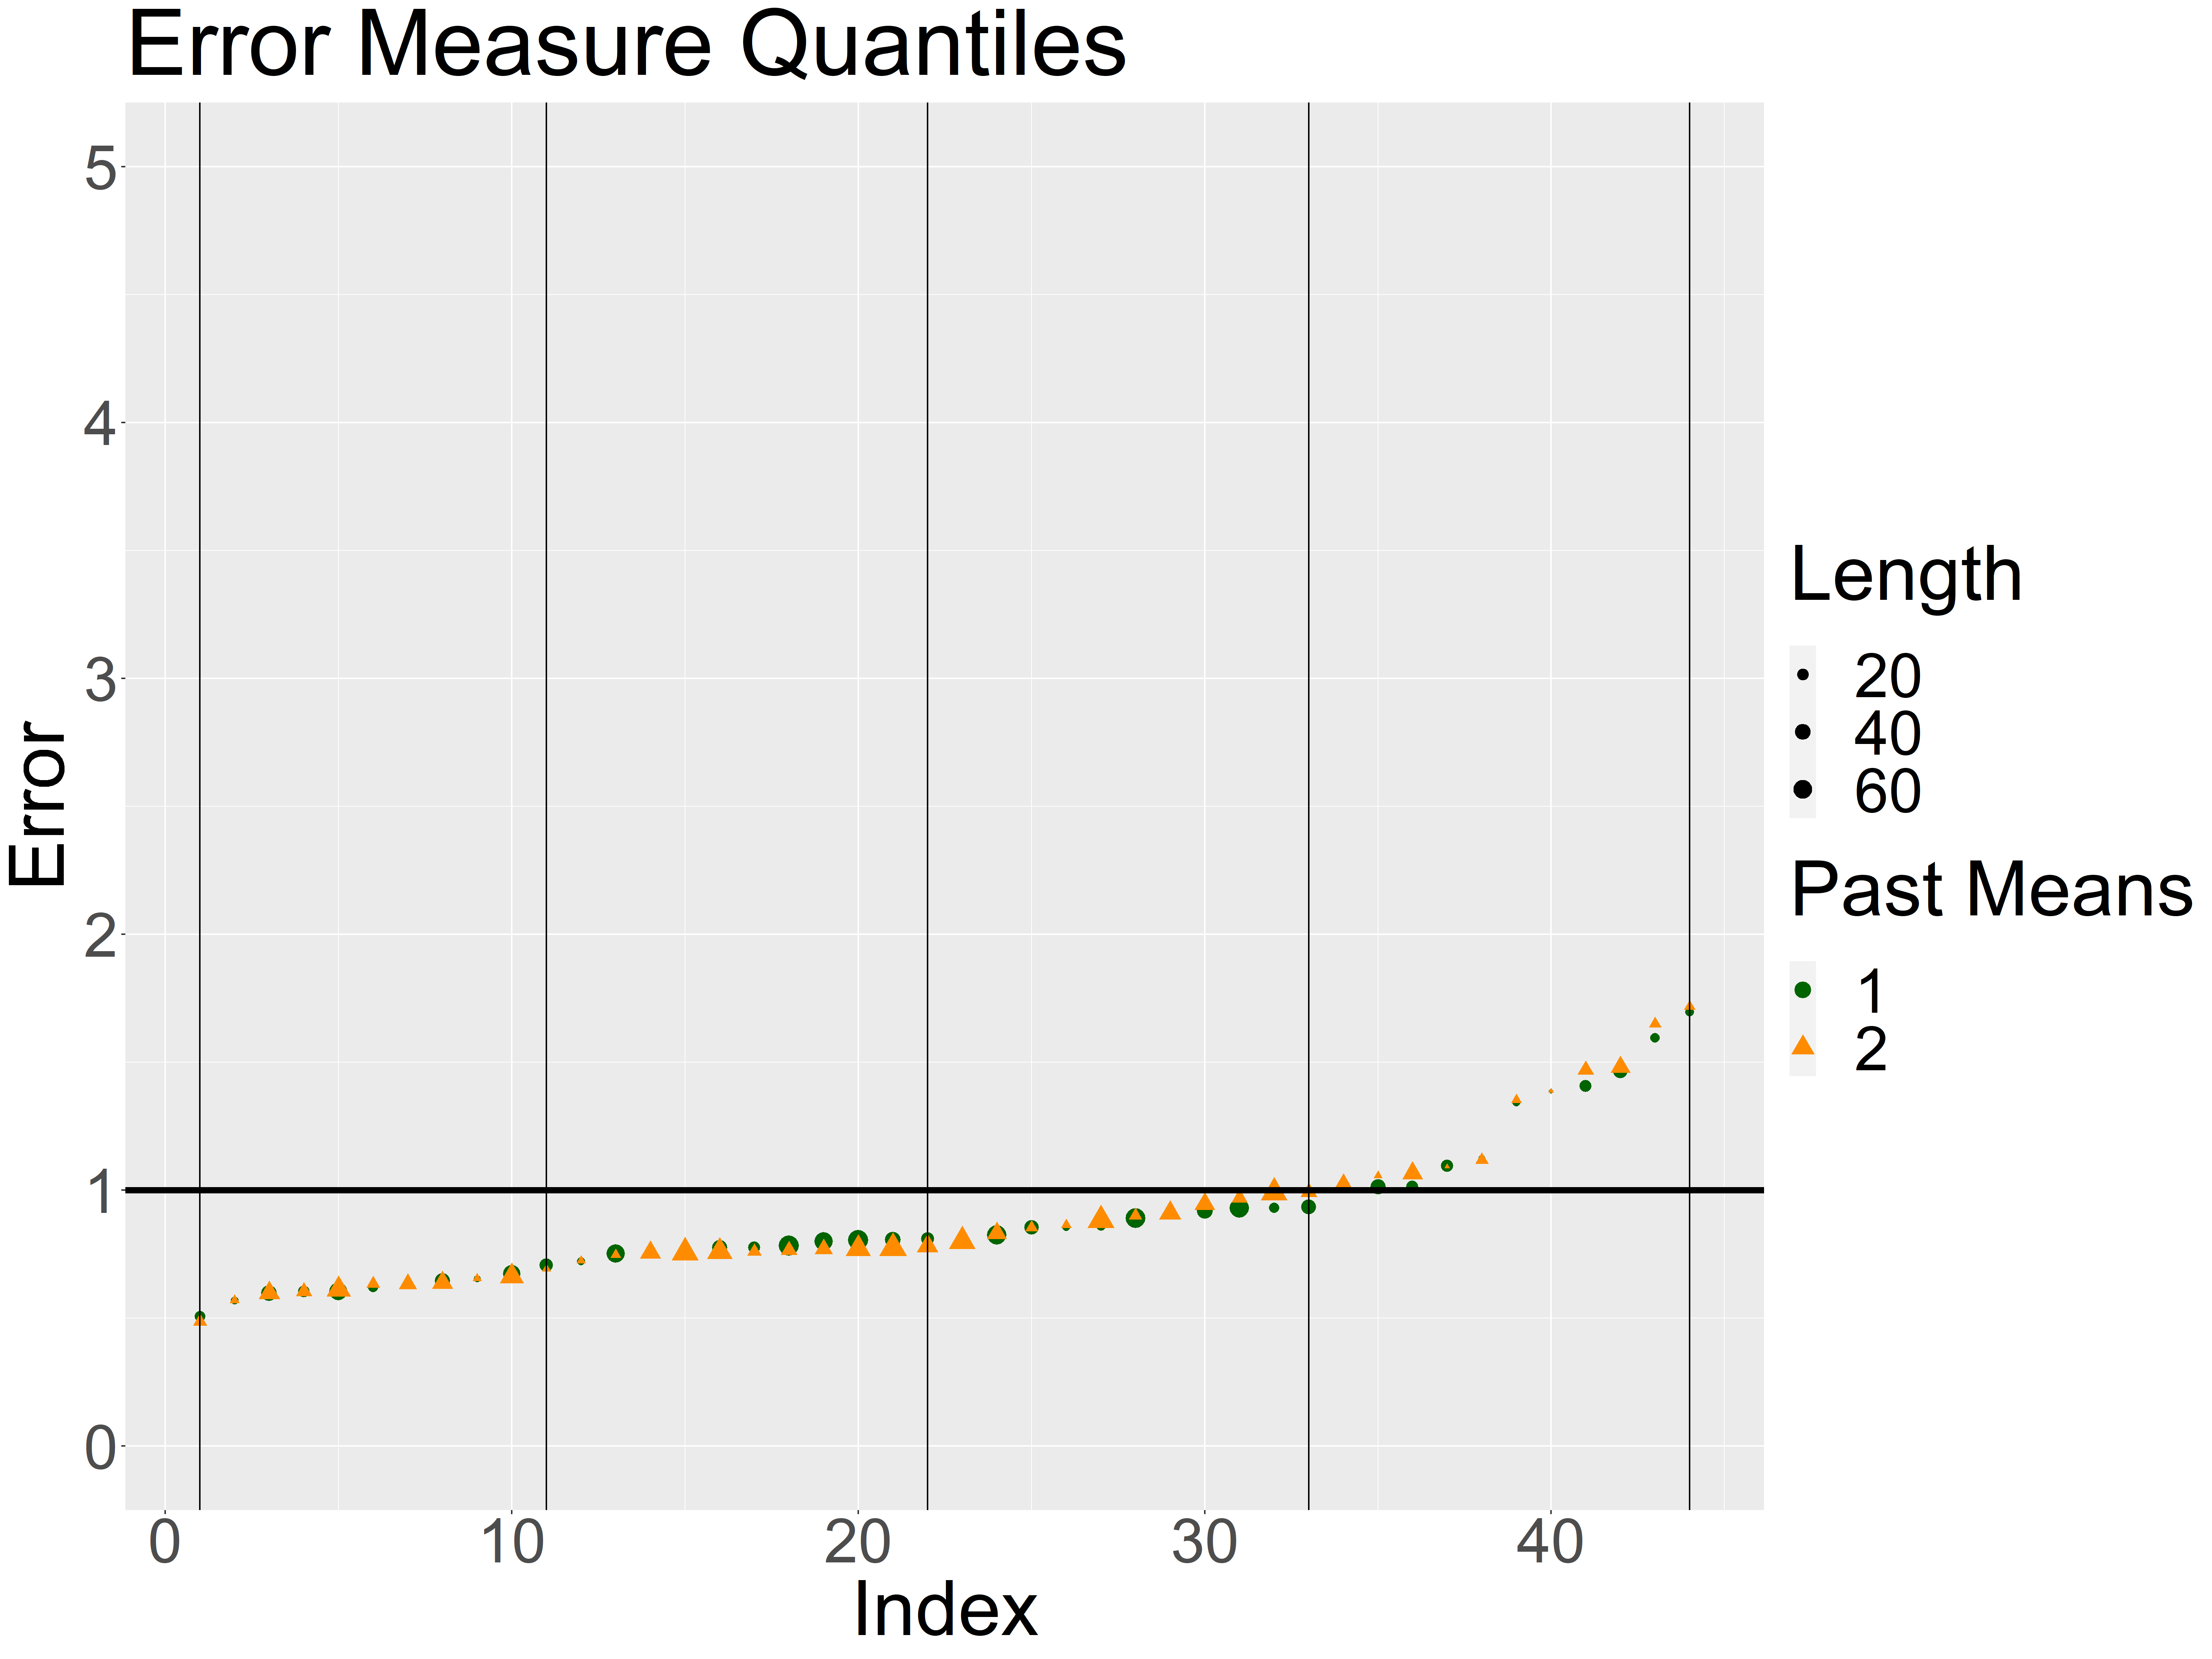
\includegraphics[width=\textwidth]{ErrorMeasureINGARCH_Quant_all__Variation_pastMean.png}
\caption{Quantiles for a different number of past means}
\label{fig:past means Quant}
\end{subfigure}
\caption{Comparison of a different number of past means}
\label{fig:past means Comp1}
\end{figure}


In figure \ref{fig:past obs Comp1} we compare the INGARCH(1,1) (red) model with the INGARCH(2,1) (blue) model. Again the performance is very similar in general. 

\begin{figure}[htb!]
\centering
\begin{subfigure}[b]{0.45\textwidth}
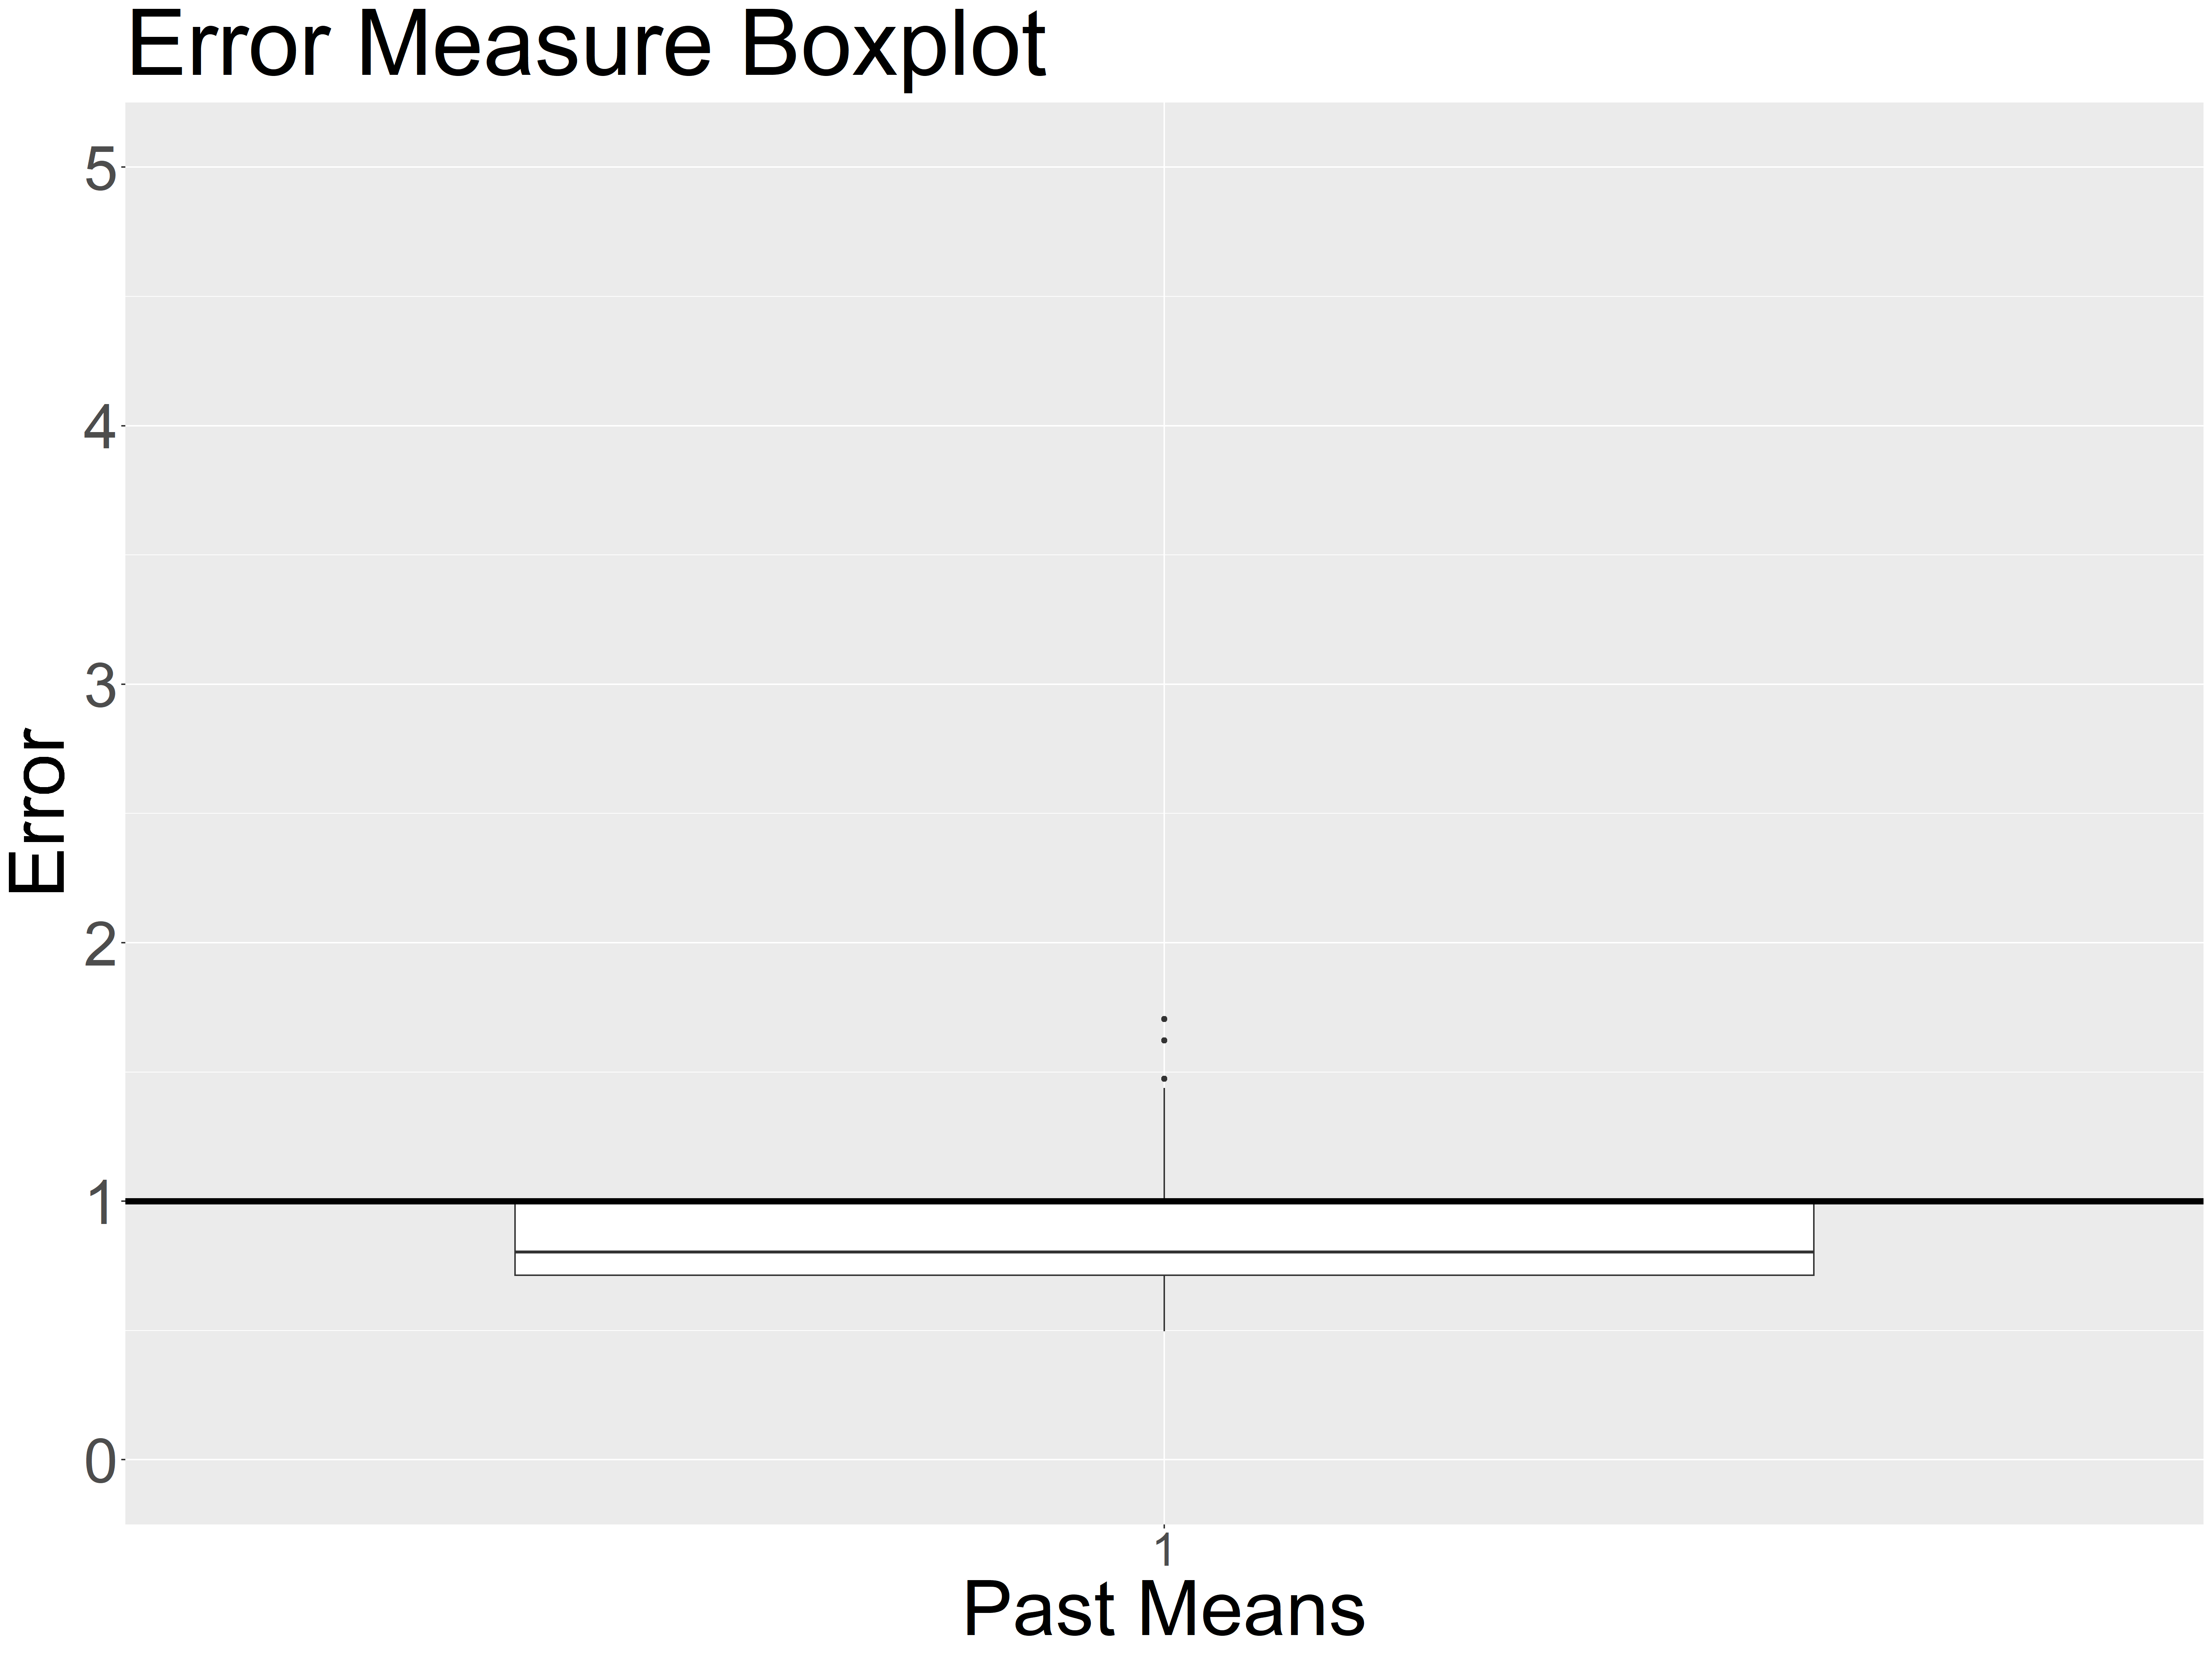
\includegraphics[width=\textwidth]{ErrorMeasureINGARCH_Box_all__Variation_pastOb.png}
\caption{Boxplot for a different number of past observations}
\label{fig:past obs Box}
\end{subfigure}
\hfill
\begin{subfigure}[b]{0.45\textwidth}
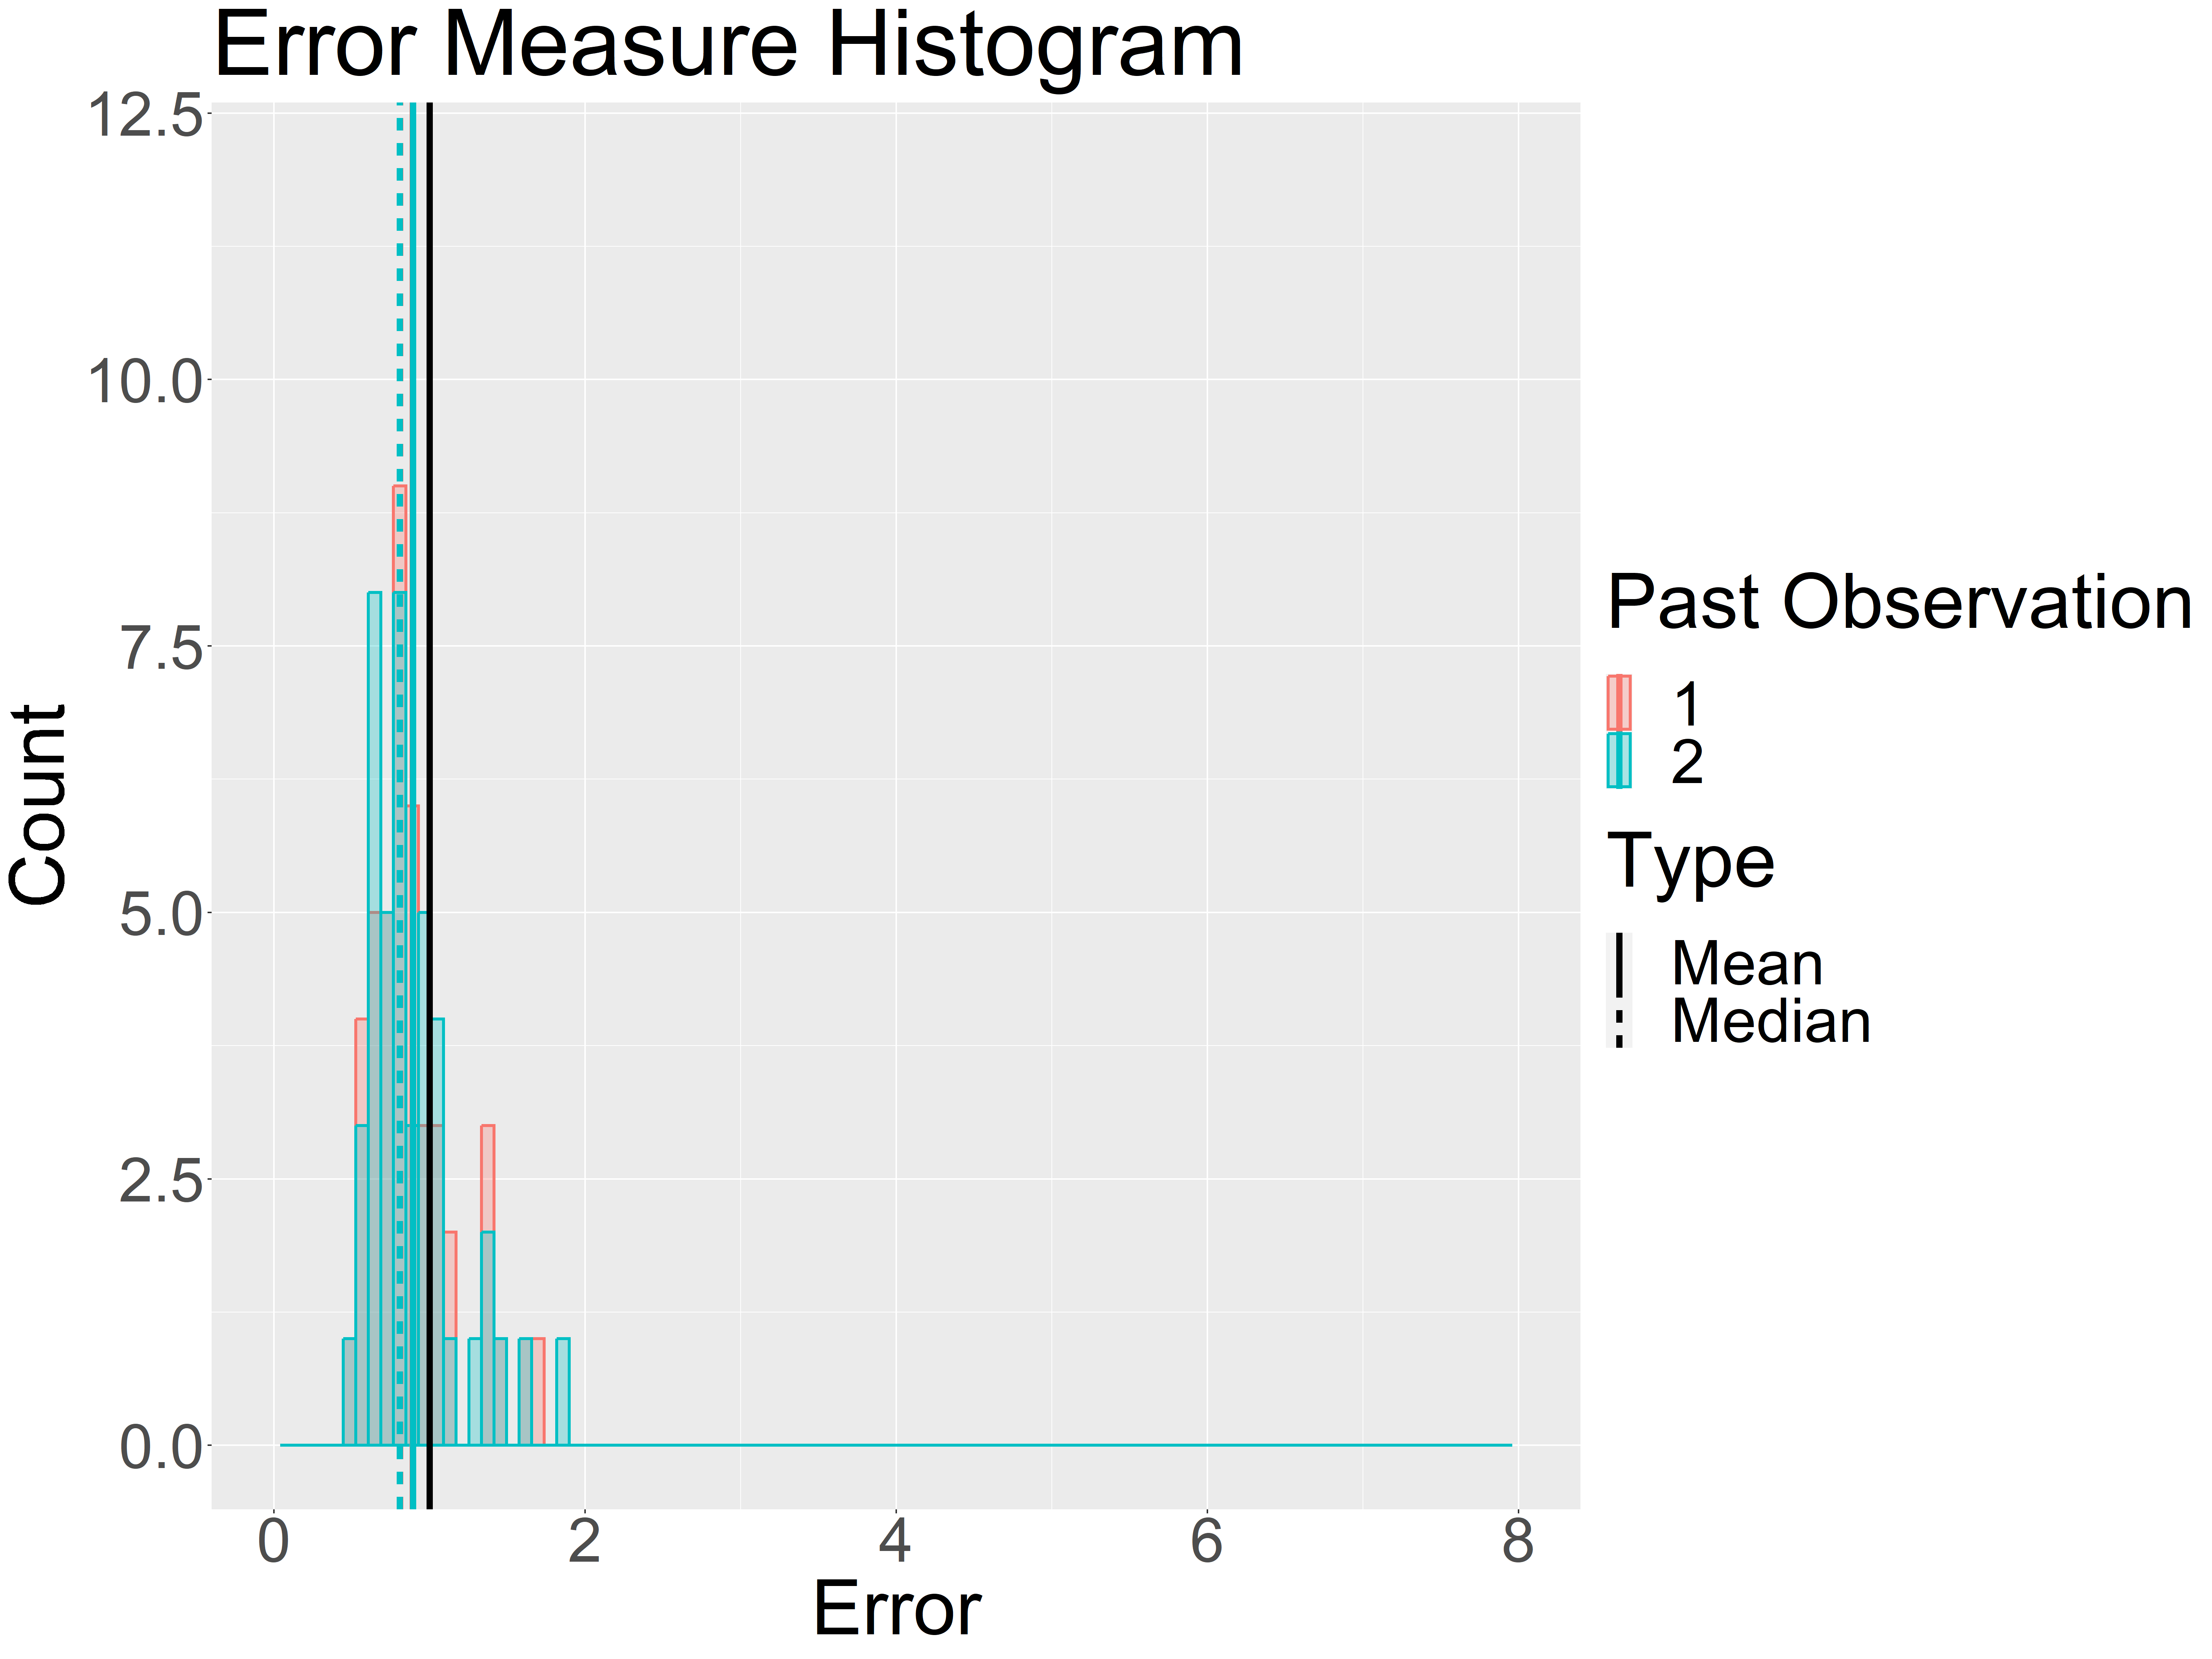
\includegraphics[width=\textwidth]{ErrorMeasureINGARCH_Histogram_all__Variation_pastOb.png}
\caption{Histogram for a different number of past observations}
\label{fig:past obs Hist}
\end{subfigure}
\hfill
\begin{subfigure}[b]{0.8\textwidth}
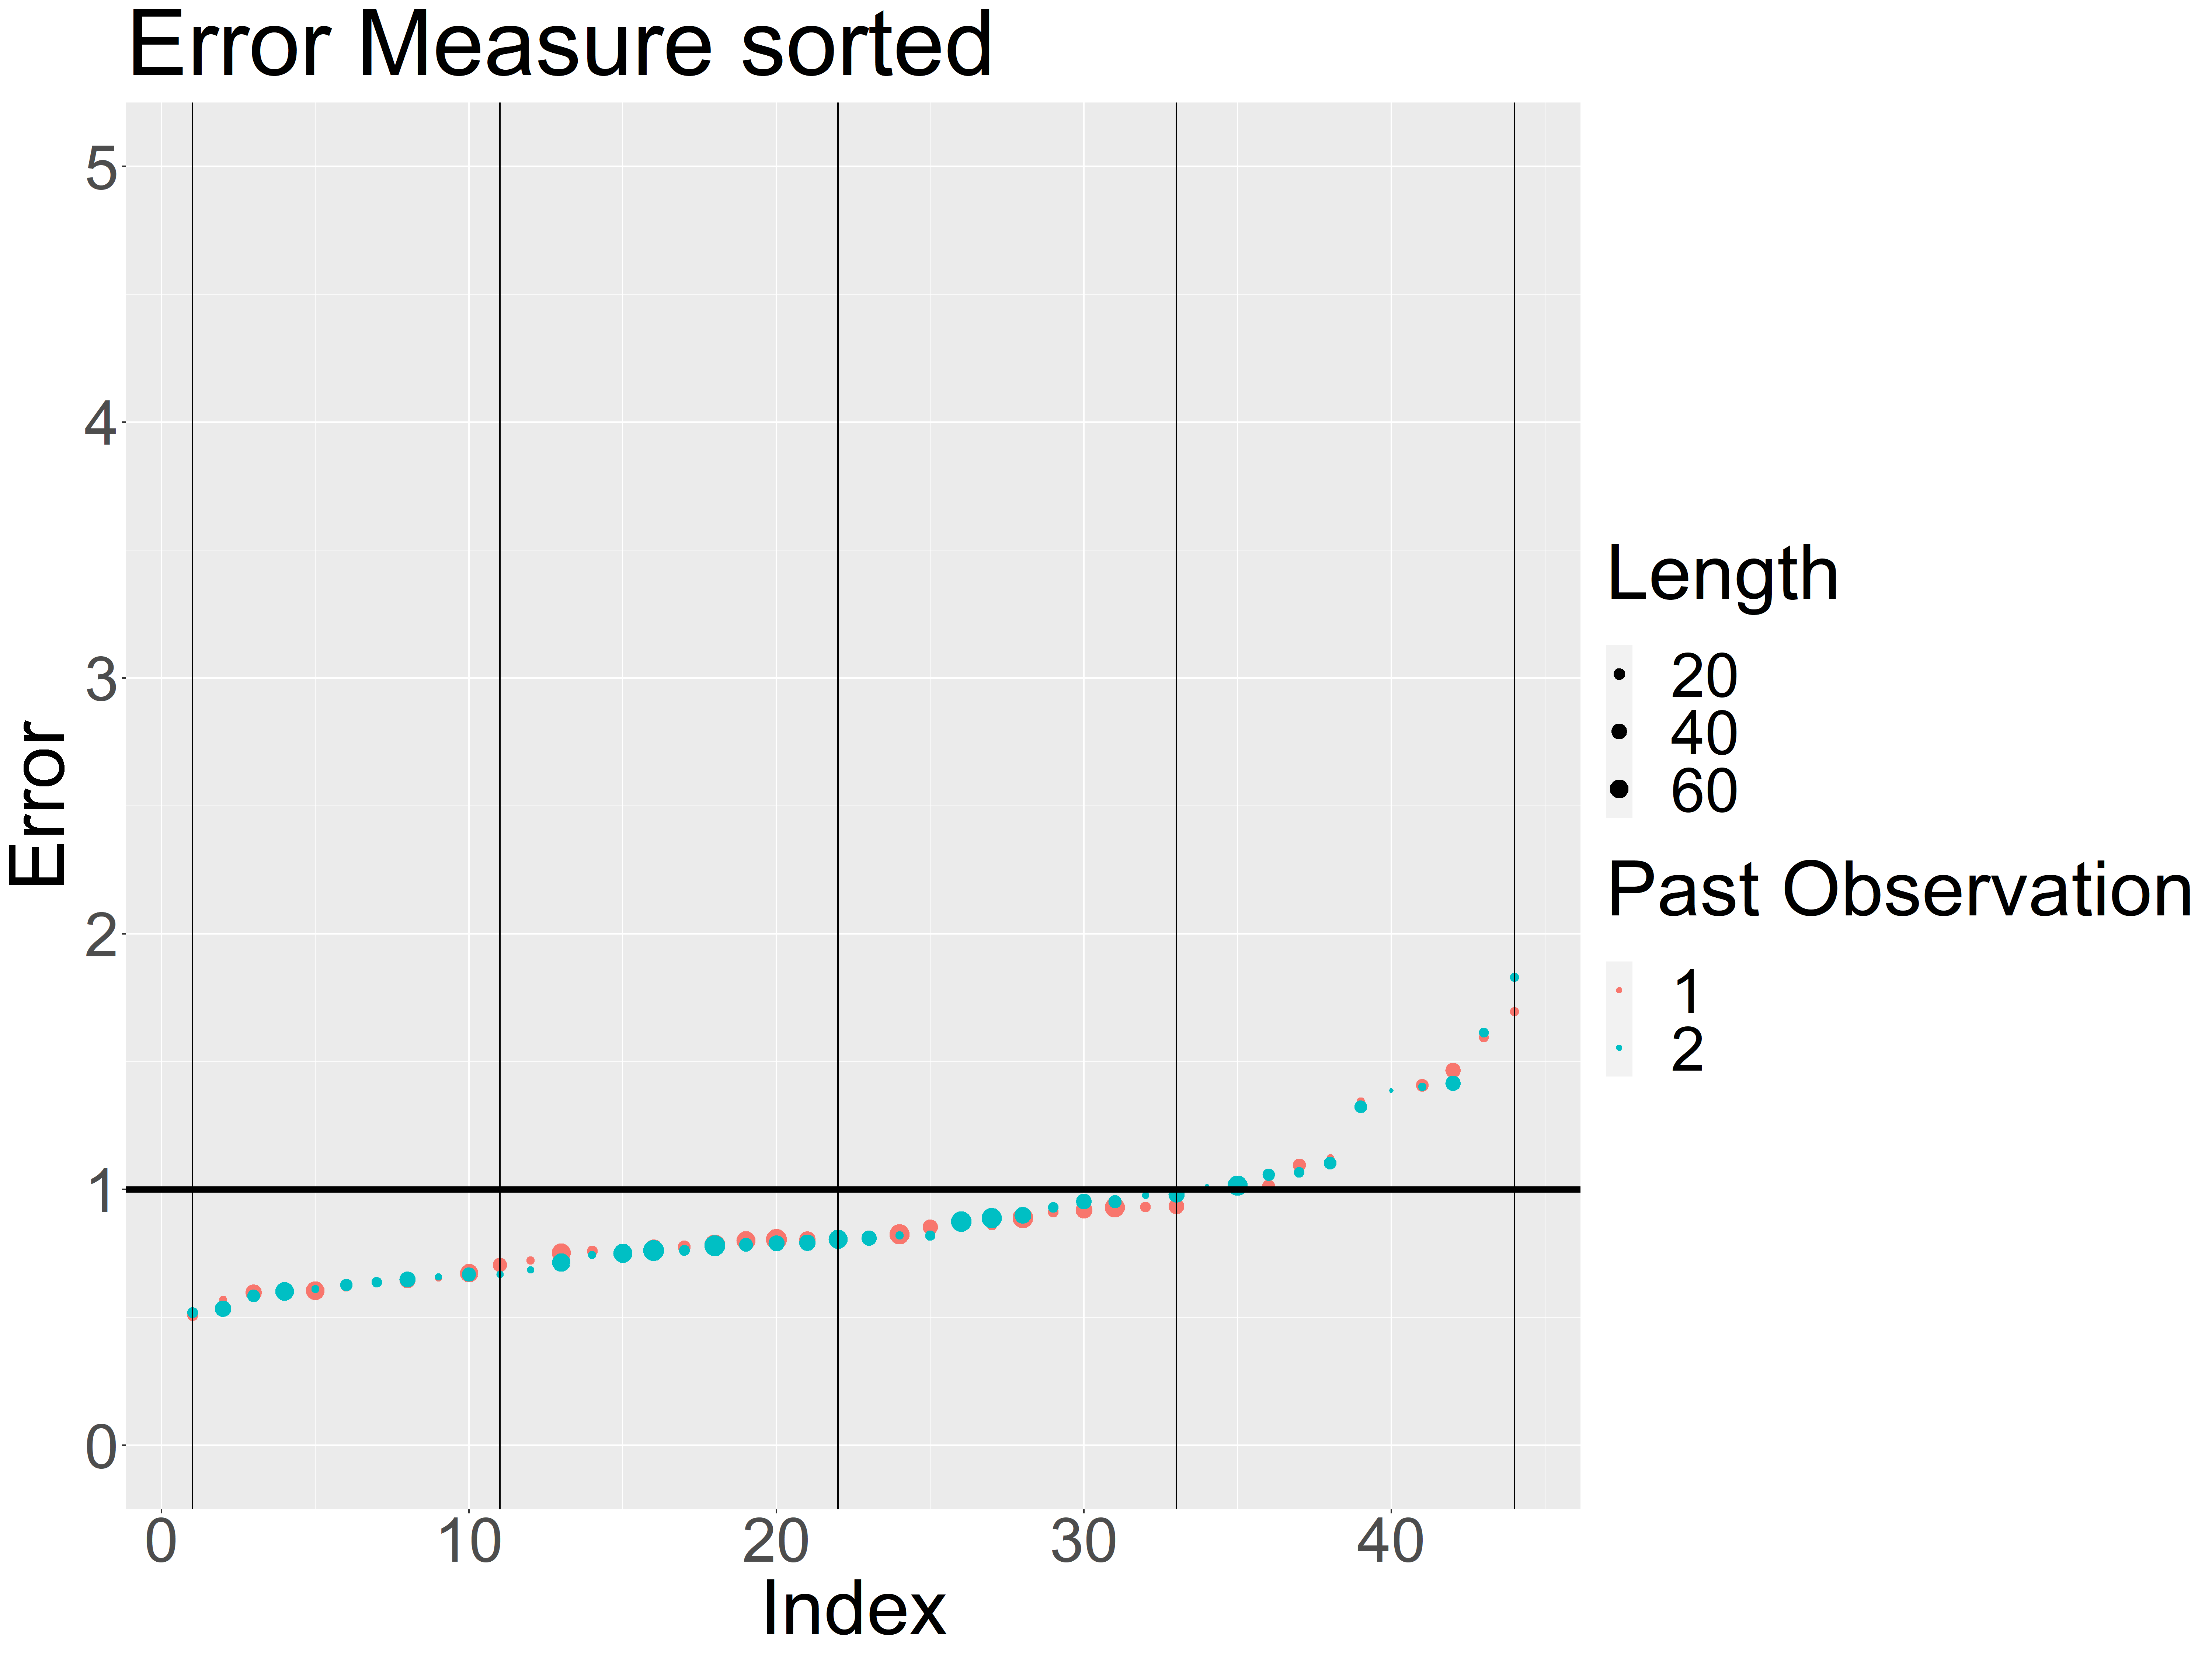
\includegraphics[width=\textwidth]{ErrorMeasureINGARCH_Quant_all__Variation_pastOb.png}
\caption{Quantiles for a different number of past observations}
\label{fig:past obs Quant}
\end{subfigure}
\caption{Comparison of a different number of past observations}
\label{fig:past obs Comp1}
\end{figure}

As we saw, there is not much difference between the INGARCH(1,1), INGARCH(2,1) and INGARCH(1,2) model. One could compare the AIC or some other measure for the different models and base their choice on that. However, this is not further explored here and hence the INGARCH(1,1) model is taken because it is the smallest.

\subsection{CoDA Specifications Results}
\label{sec: CoDA Specifications Results}

Last, we will compare different CoDA Specifications as mentioned in \ref{sec: Coda Specifications}. Like above we choose one standard model for comparison and always only change one setting. For CoDA our standard model uses extending windows, the full history $h=1$, an initial window length of $w=0.5$, use the simple replacement strategy with $\delta=0.1$, no $\Tsp$-spaces and the one-vs-all method. 

\subsection{Zero Handling}
\label{sec: Zero Handling}

First we compare the different options of handling zeros as explained in \ref{sec: Coda Specifications}. The results are shown in figure \ref{fig:Coda zero handling Comp1}. It seems that the simple replacement strategy with $\delta_j = 0.1$, $\forall j$ results in marginally better performance.

\begin{figure}[htb!]
\centering
\begin{subfigure}[b]{0.45\textwidth}
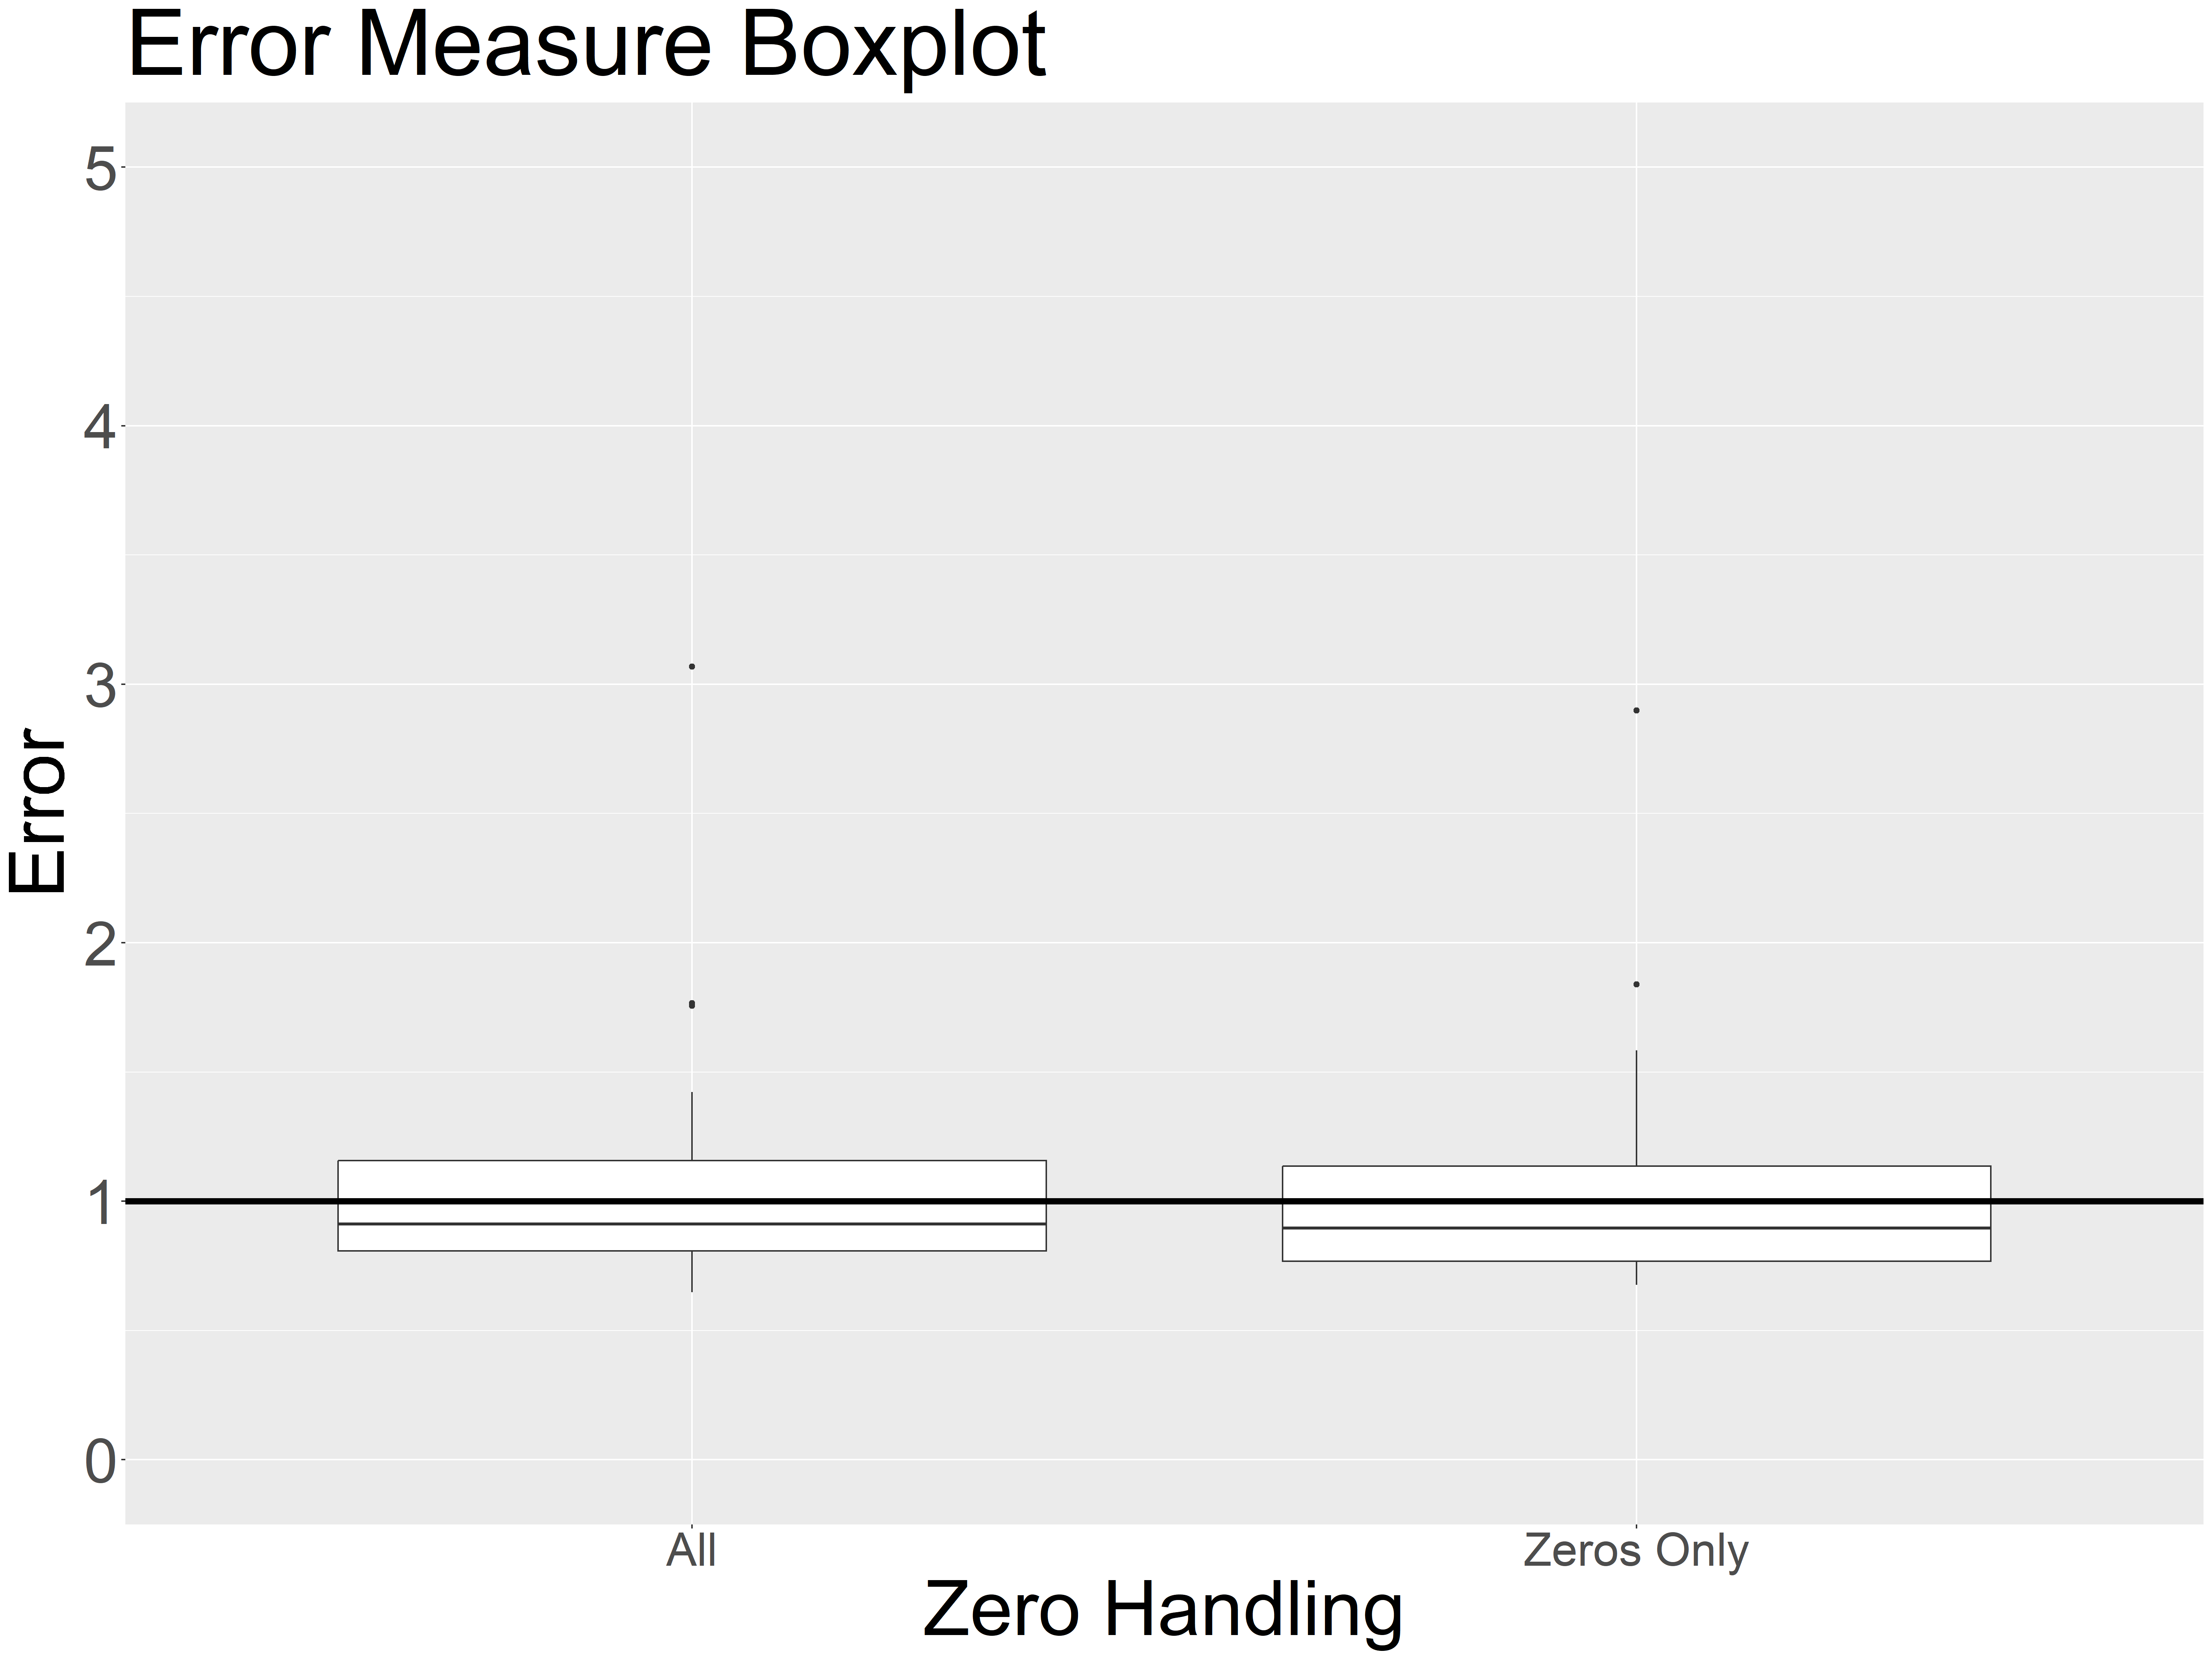
\includegraphics[width=\textwidth]{ErrorMeasureCoDA_Box_all__Variation_zeroHandling.png}
\caption{Boxplot for a different methods of zero handling}
\label{fig:Coda zero handling Box}
\end{subfigure}
\hfill
\begin{subfigure}[b]{0.45\textwidth}
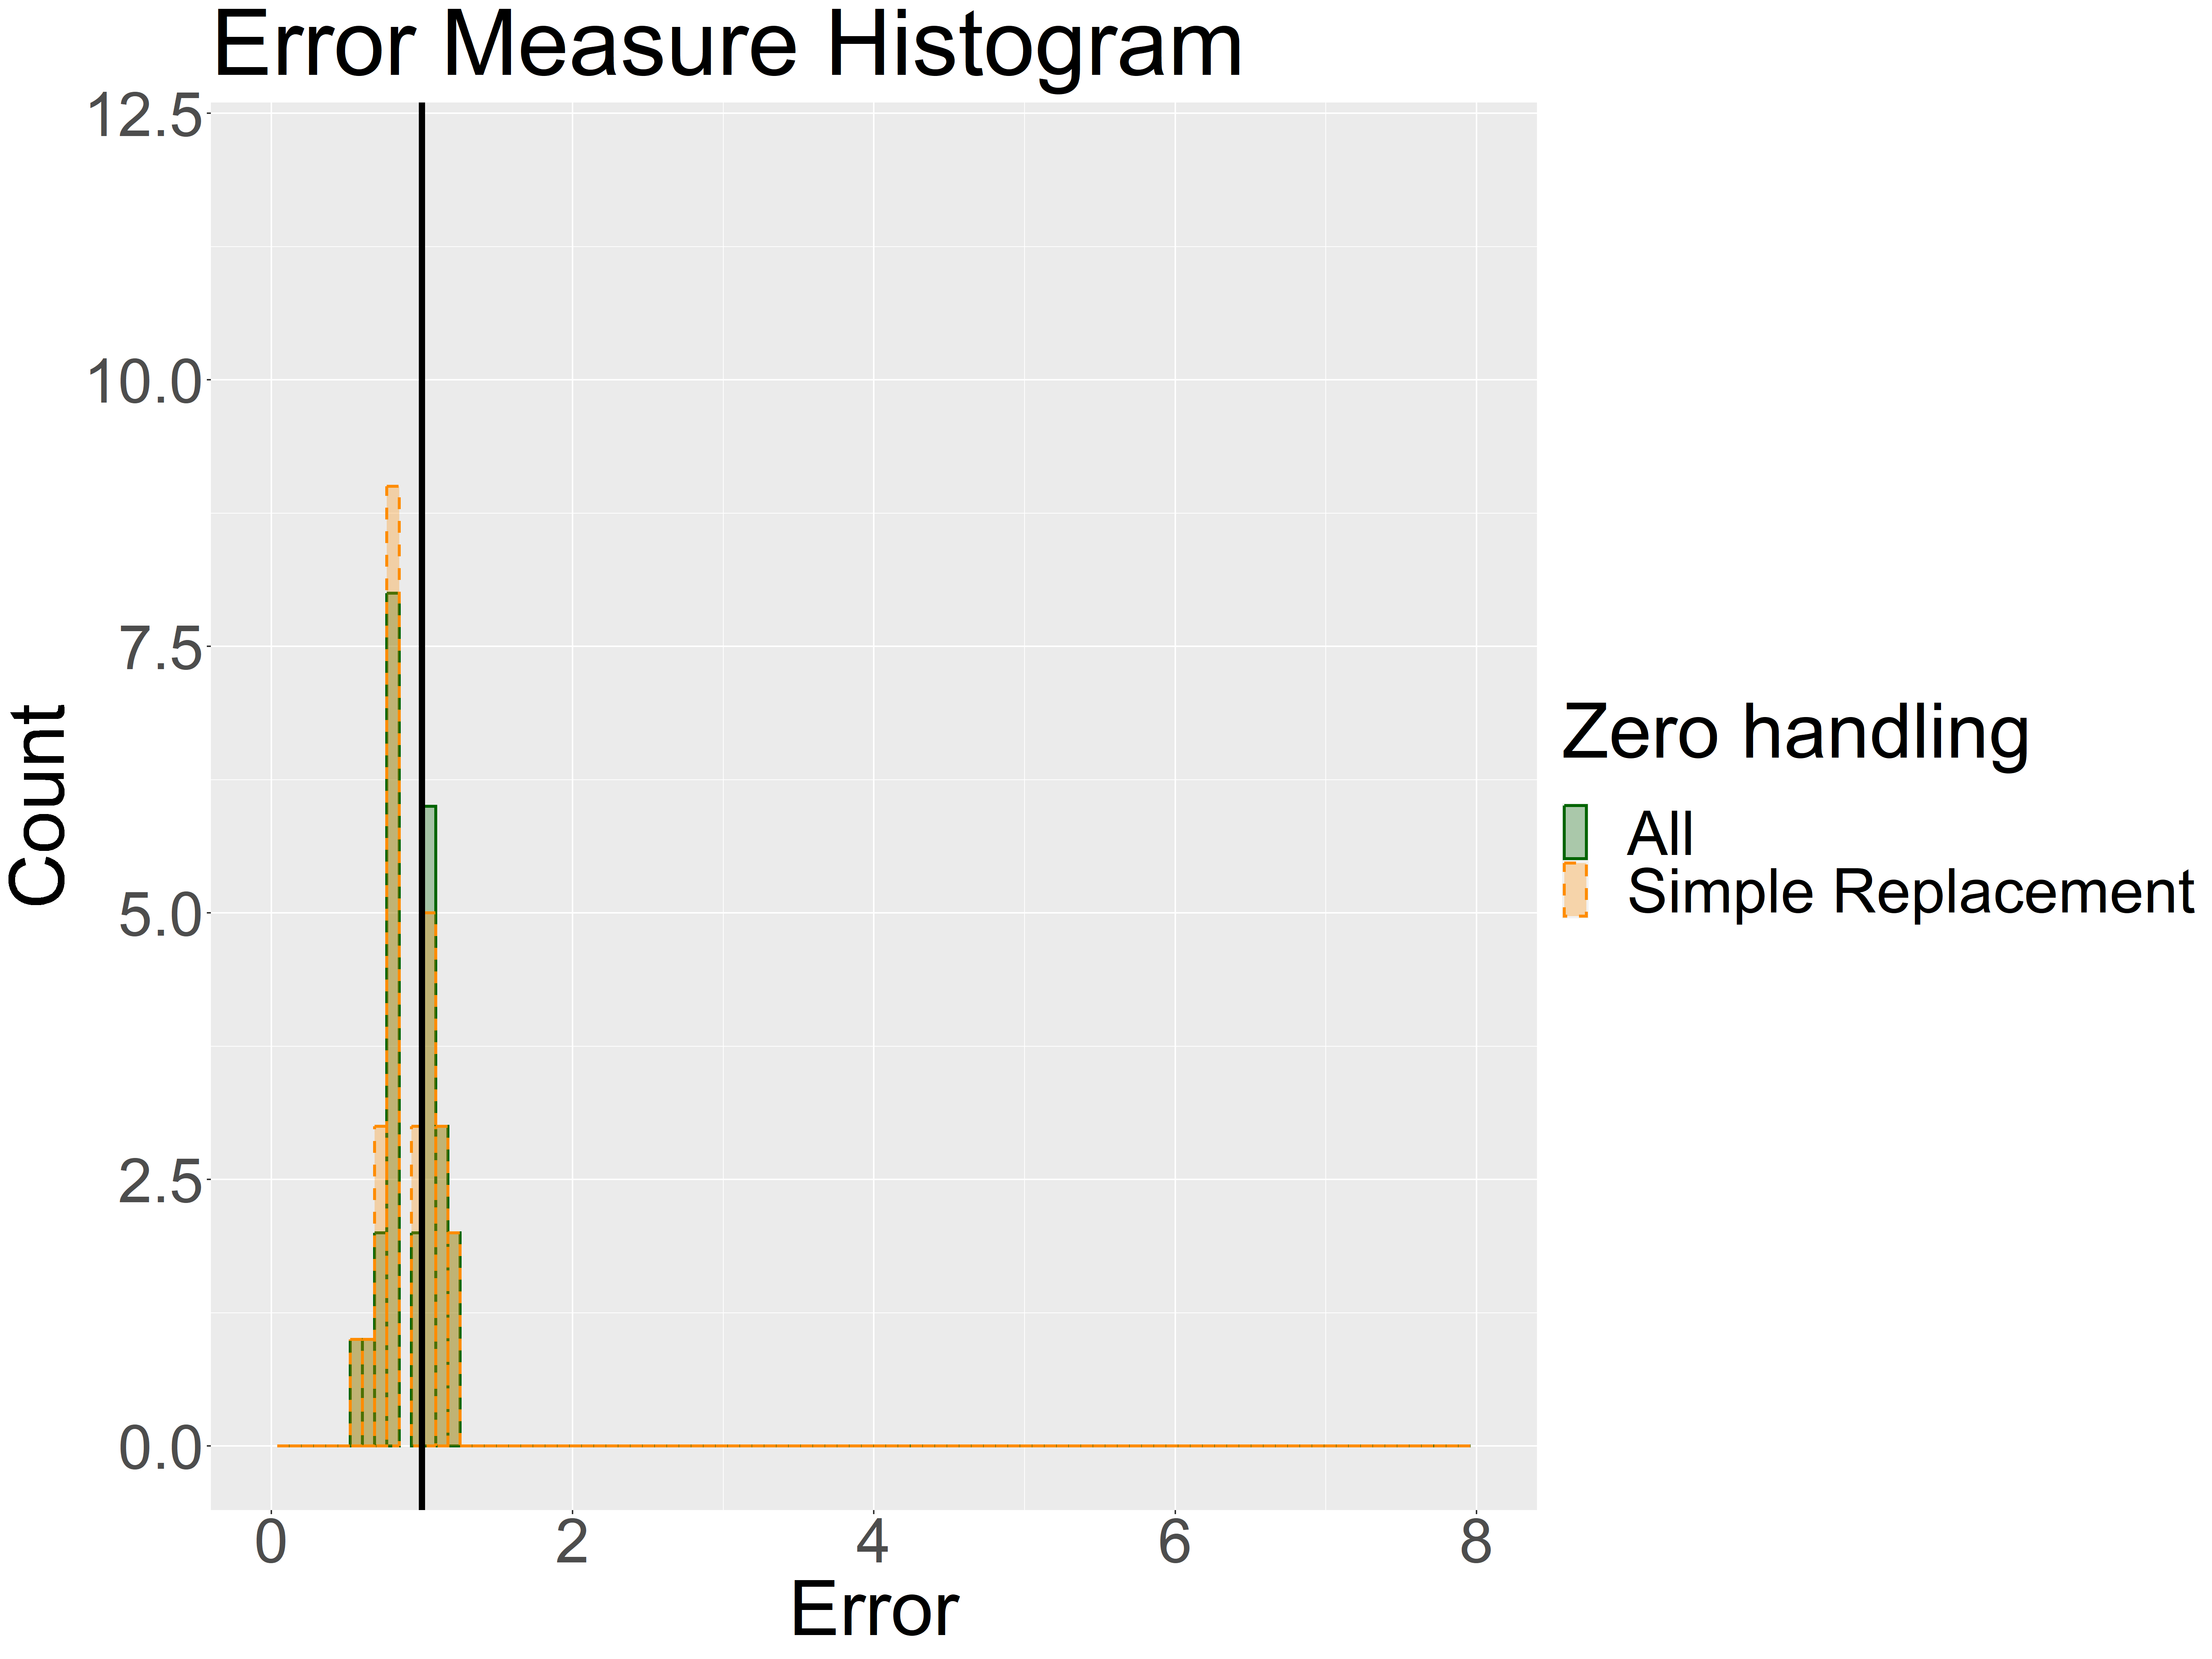
\includegraphics[width=\textwidth]{ErrorMeasureCoDA_Histogram_all__Variation_zeroHandling.png}
\caption{Histogram for a different methods of zero handling}
\label{fig:Coda zero handling Hist}
\end{subfigure}
\hfill
\begin{subfigure}[b]{0.8\textwidth}
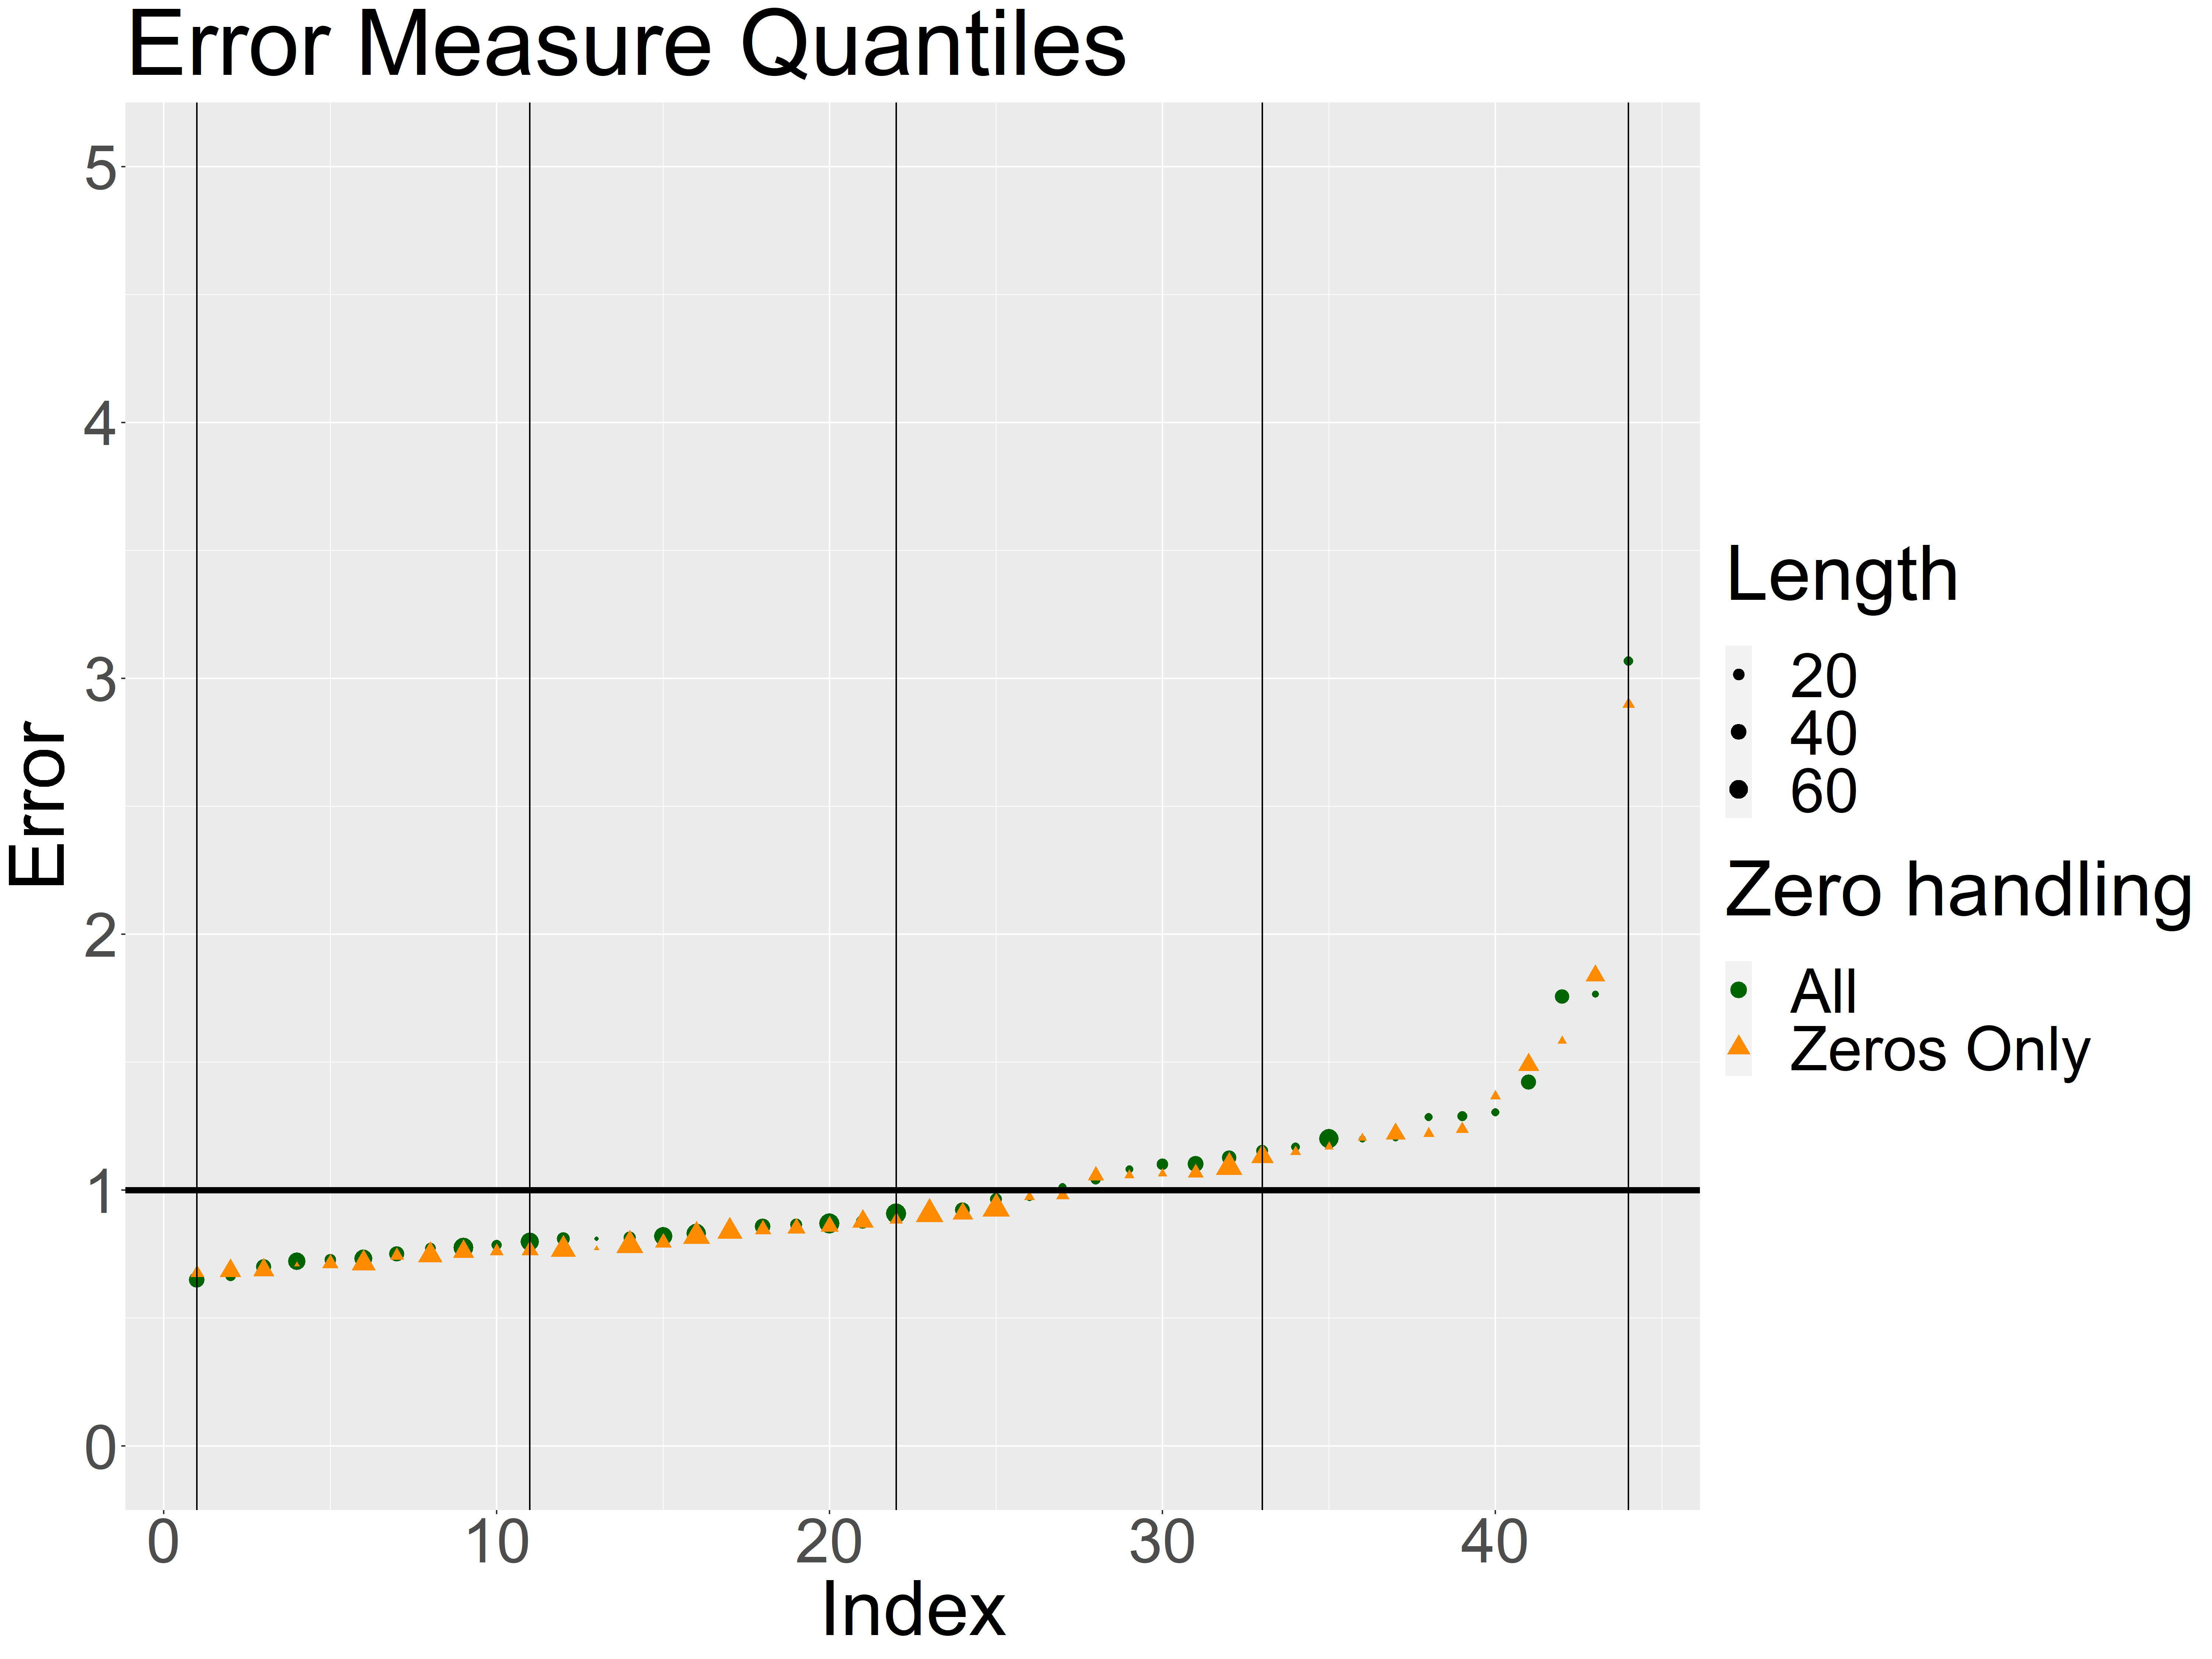
\includegraphics[width=\textwidth]{ErrorMeasureCoDA_Quant_all__Variation_zeroHandling.png}
\caption{Quantiles for a different methods of zero handling}
\label{fig:Coda zero handling Quant}
\end{subfigure}
\caption{Comparison of different zero handling methods}
\label{fig:Coda zero handling Comp1}
\end{figure}

For the simple replacement strategy, one can also vary the parameter $\delta$. In figure \ref{fig:ErrorMeasureCoDA_Box_all__Variation_dL} we plotted the results for $\delta=0.01,0.1,0.5$. While the difference don't seem big at first, when we calculate the error measure only for category 4, the category with most zeros, we can see a drastic rise in performance \ref{fig:ErrorMeasureCoDA_Box_all__Variation_dLcat4}. For smaller values of $\delta$ we get better results. 

%One possible remedy to this problem is to vary the value of $\delta$ in the simple replacement method \ref{eq:simple replacement strategy}. While for the above results we used $\delta = 0.5$, in figure \ref{fig:ErrorMeasureCoDA_Box_all__Variation_dLcat4} one can see that we get considerable better results if we use a smaller $\delta$ value. With those configurations, CoDA predicts zero values faster than before however, the difference in total is not huge as seen in figure \ref{fig:ErrorMeasureCoDA_Box_all__Variation_dL} since after all, the absolute difference is only 1 in most cases.

\begin{figure}[htbp]
	\centering
		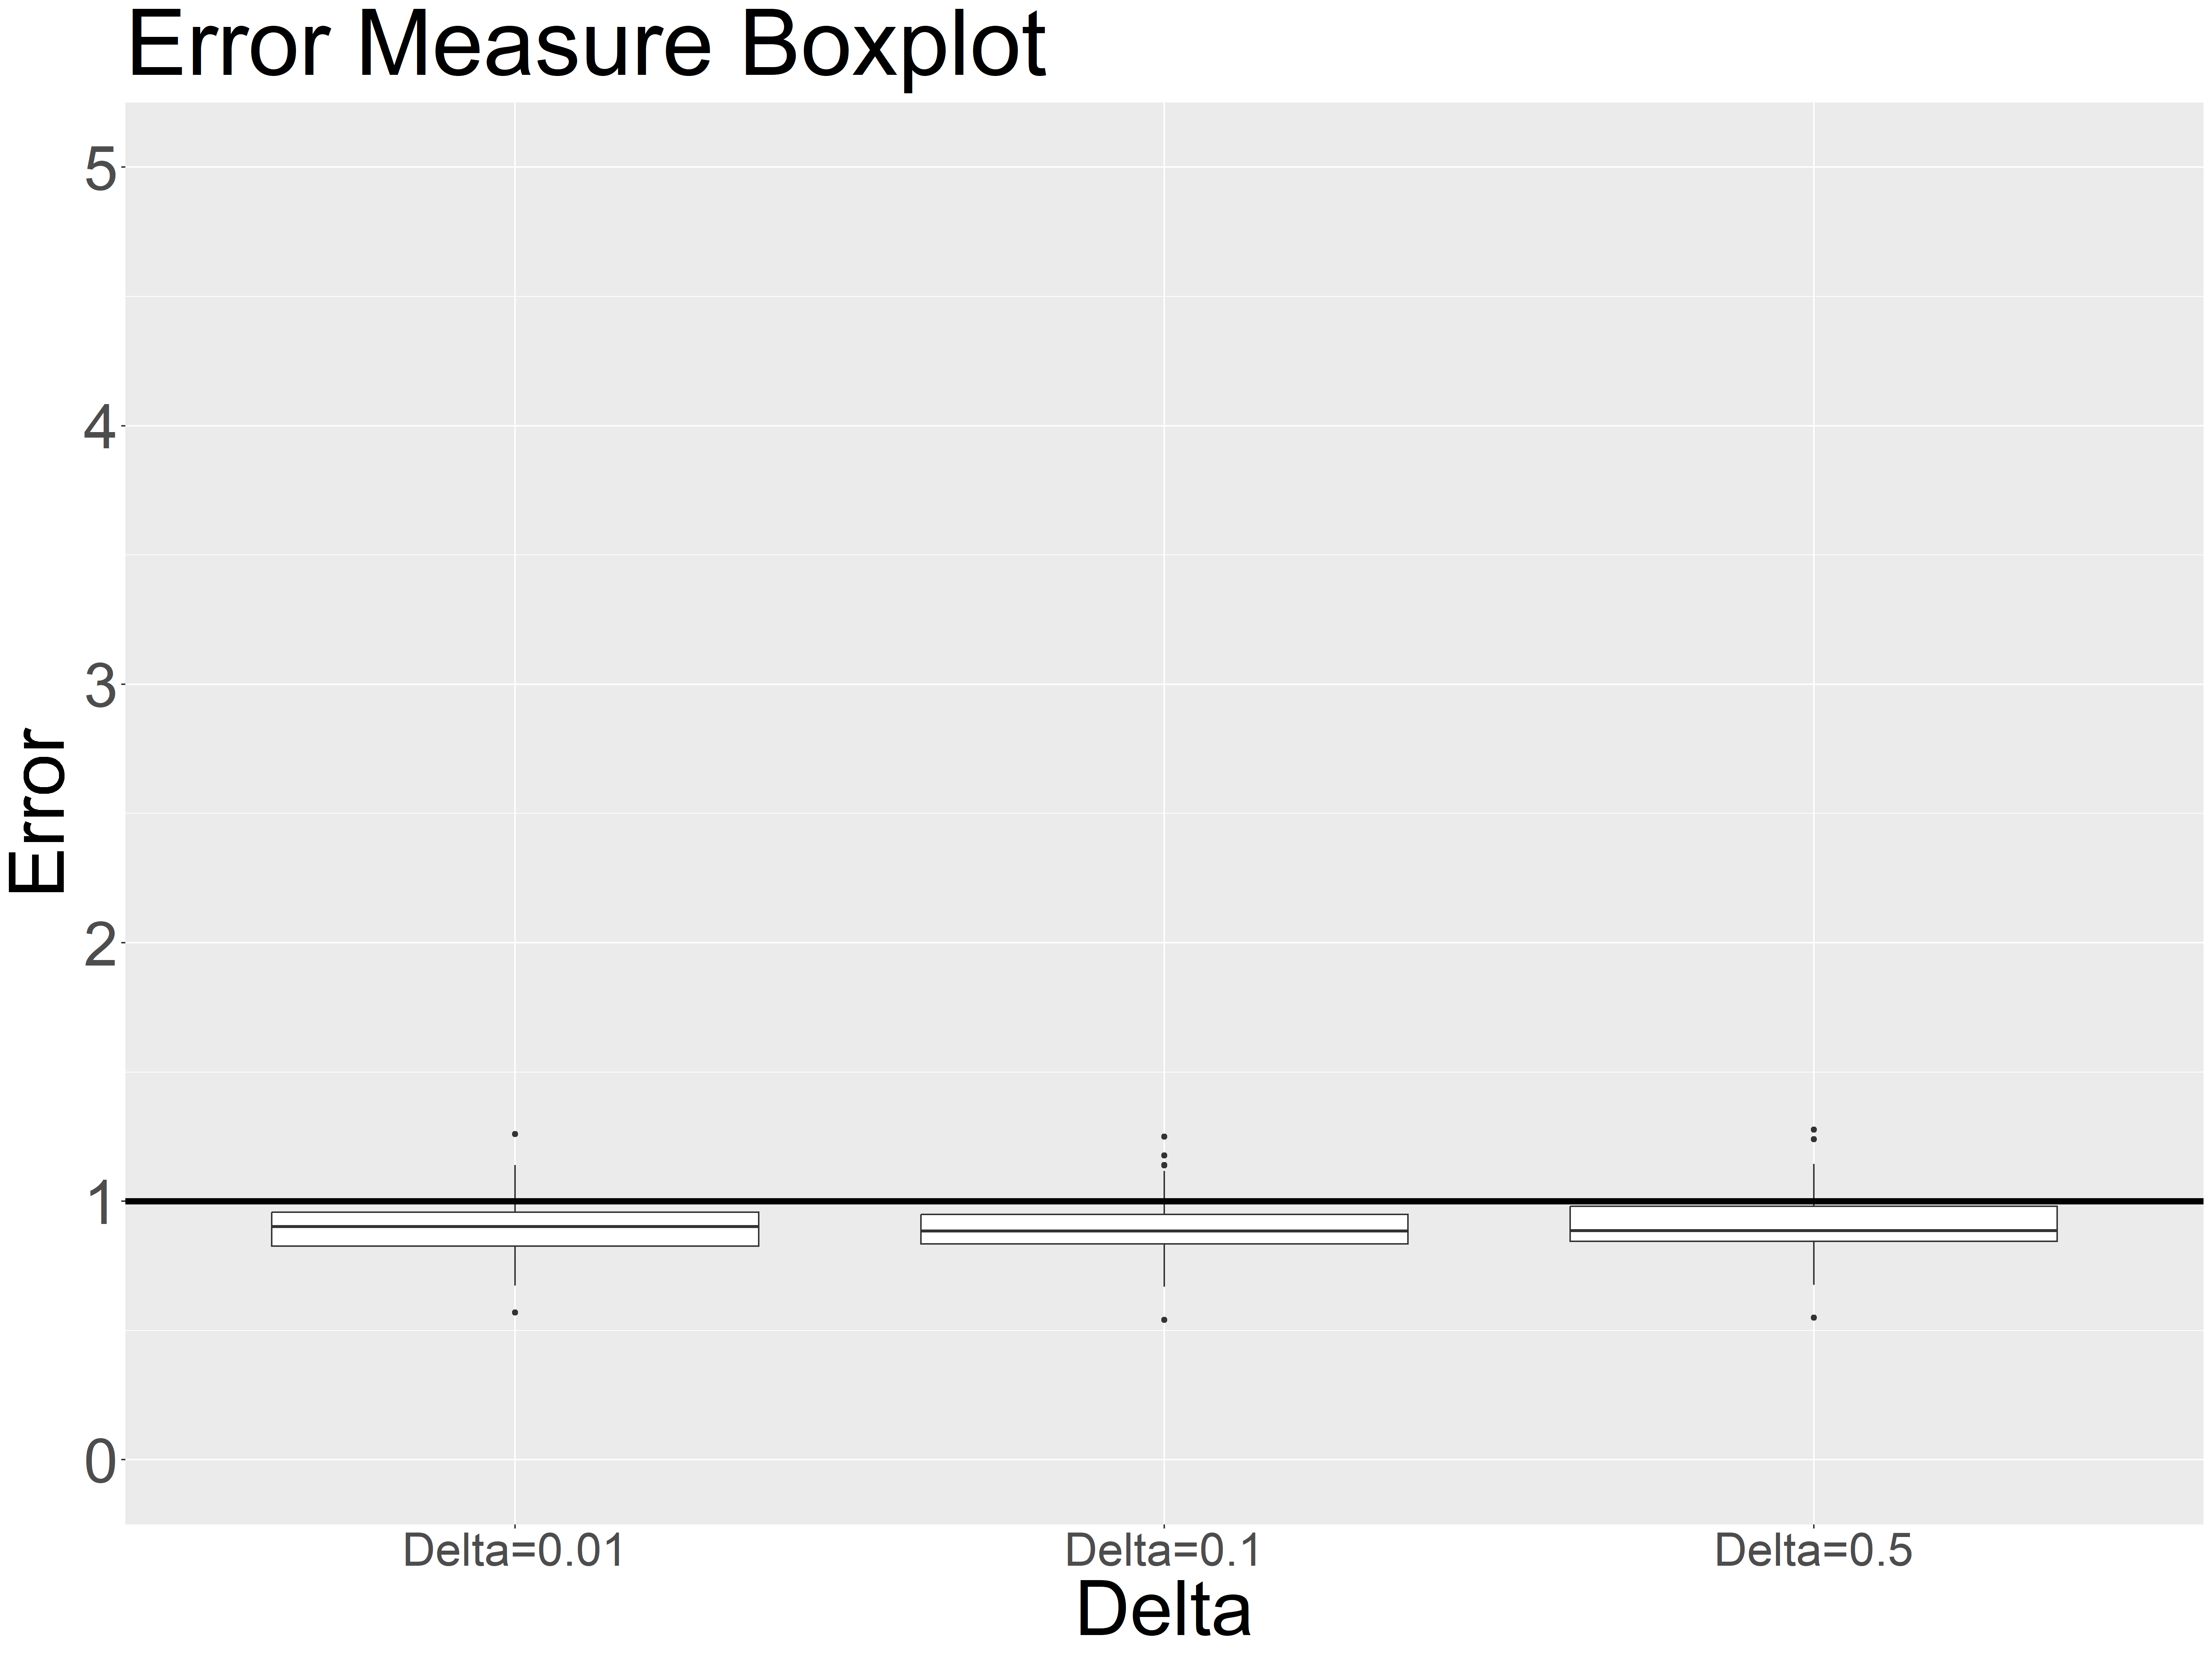
\includegraphics[width=0.80\textwidth]{Graphiken/ErrorMeasureCoDA_Box_all__Variation_dL.png}
	\caption{Error Measure for all categories}
	\label{fig:ErrorMeasureCoDA_Box_all__Variation_dL}
\end{figure}

\begin{figure}[htbp]
	\centering
		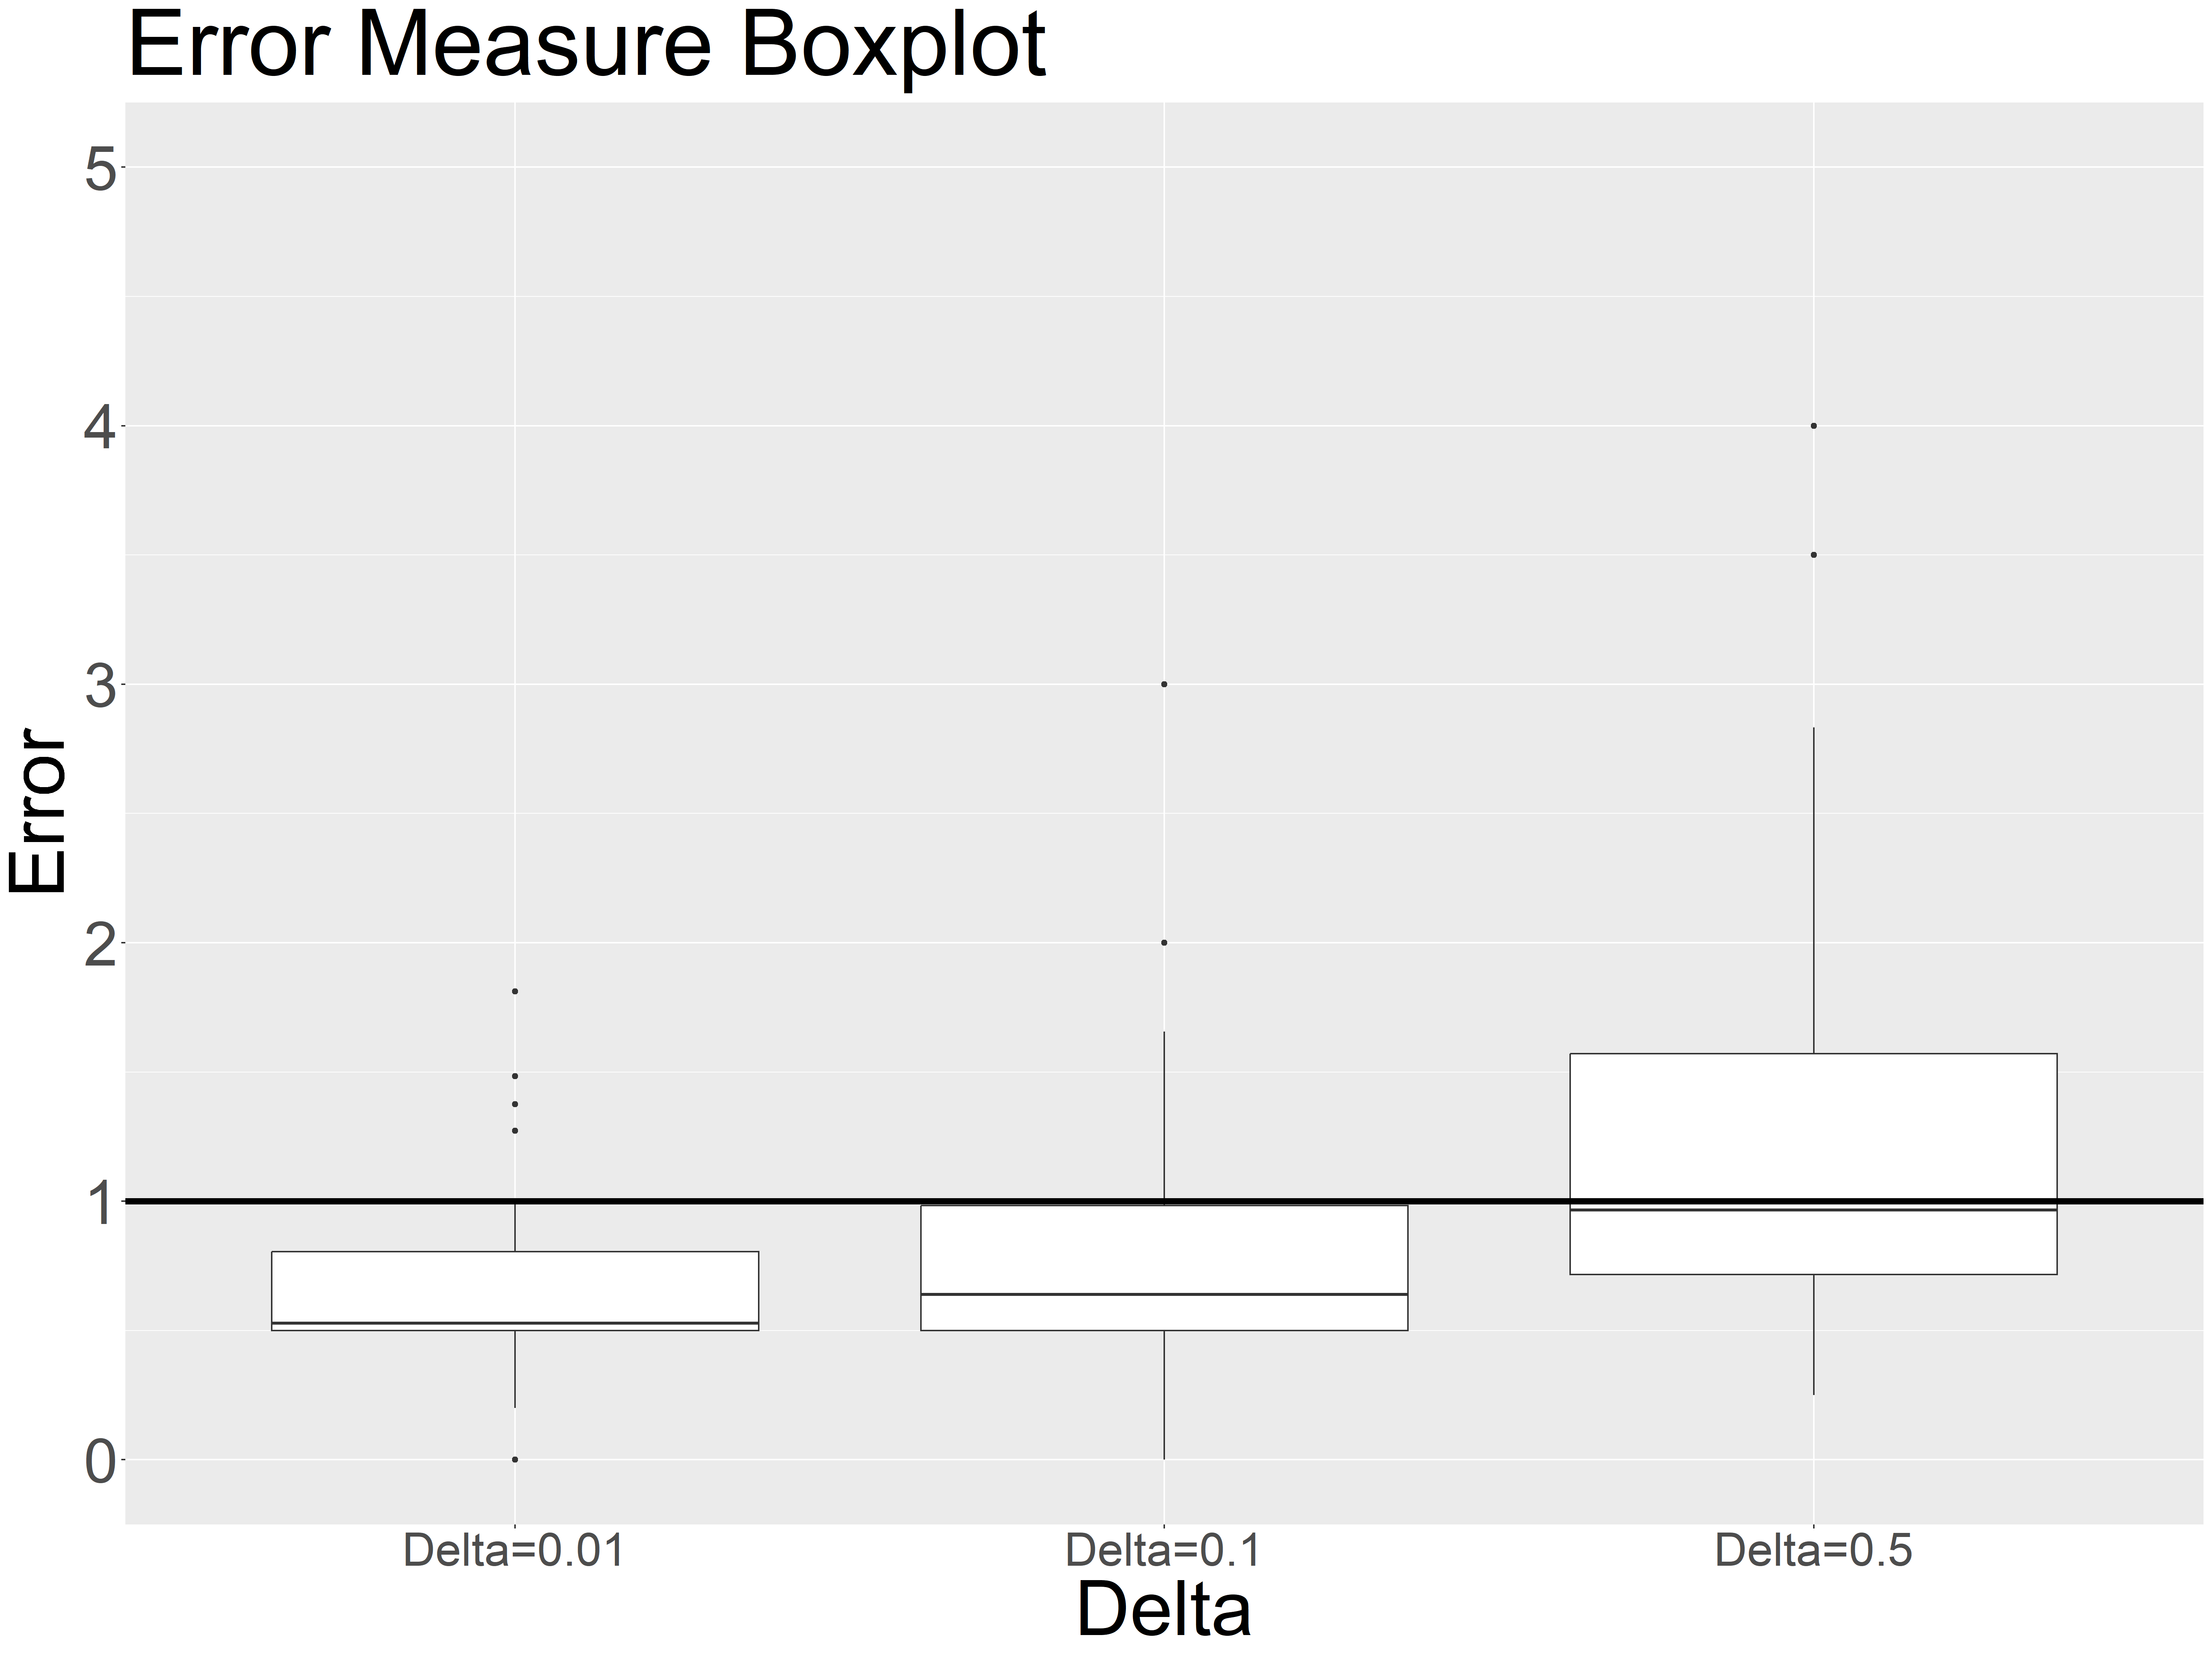
\includegraphics[width=0.80\textwidth]{Graphiken/ErrorMeasureCoDA_Box_all__Variation_dLcat4.png}
	\caption{Error Measure for Category 4}
	\label{fig:ErrorMeasureCoDA_Box_all__Variation_dLcat4}
\end{figure}



To further investigate the differences, we look in detail at the time series with the highest error measures for $\delta=0.5$. The fridge with the highest error is 100402 \ref{fig:Coda_Timeseries_ID100402}. We can see that for $\delta=0.5$ in category 4, the predictions stay at 1, even after a repeated amount of zero values. With the smaller $\delta$-values on the other hand, CoDA starts to predict zero values after one or two time points. While the absolute difference is only one, the error measure is so high because the naive random walk model predicts all values correctly as zero and therefore the nominator in equation \ref{eq: Error Measure Subsets} is theoretically zero. In practice, we implemented a fail-safe and set the nominator to 1e-6 to avoid division by 0. 


\begin{figure}[htbp]
	\centering
		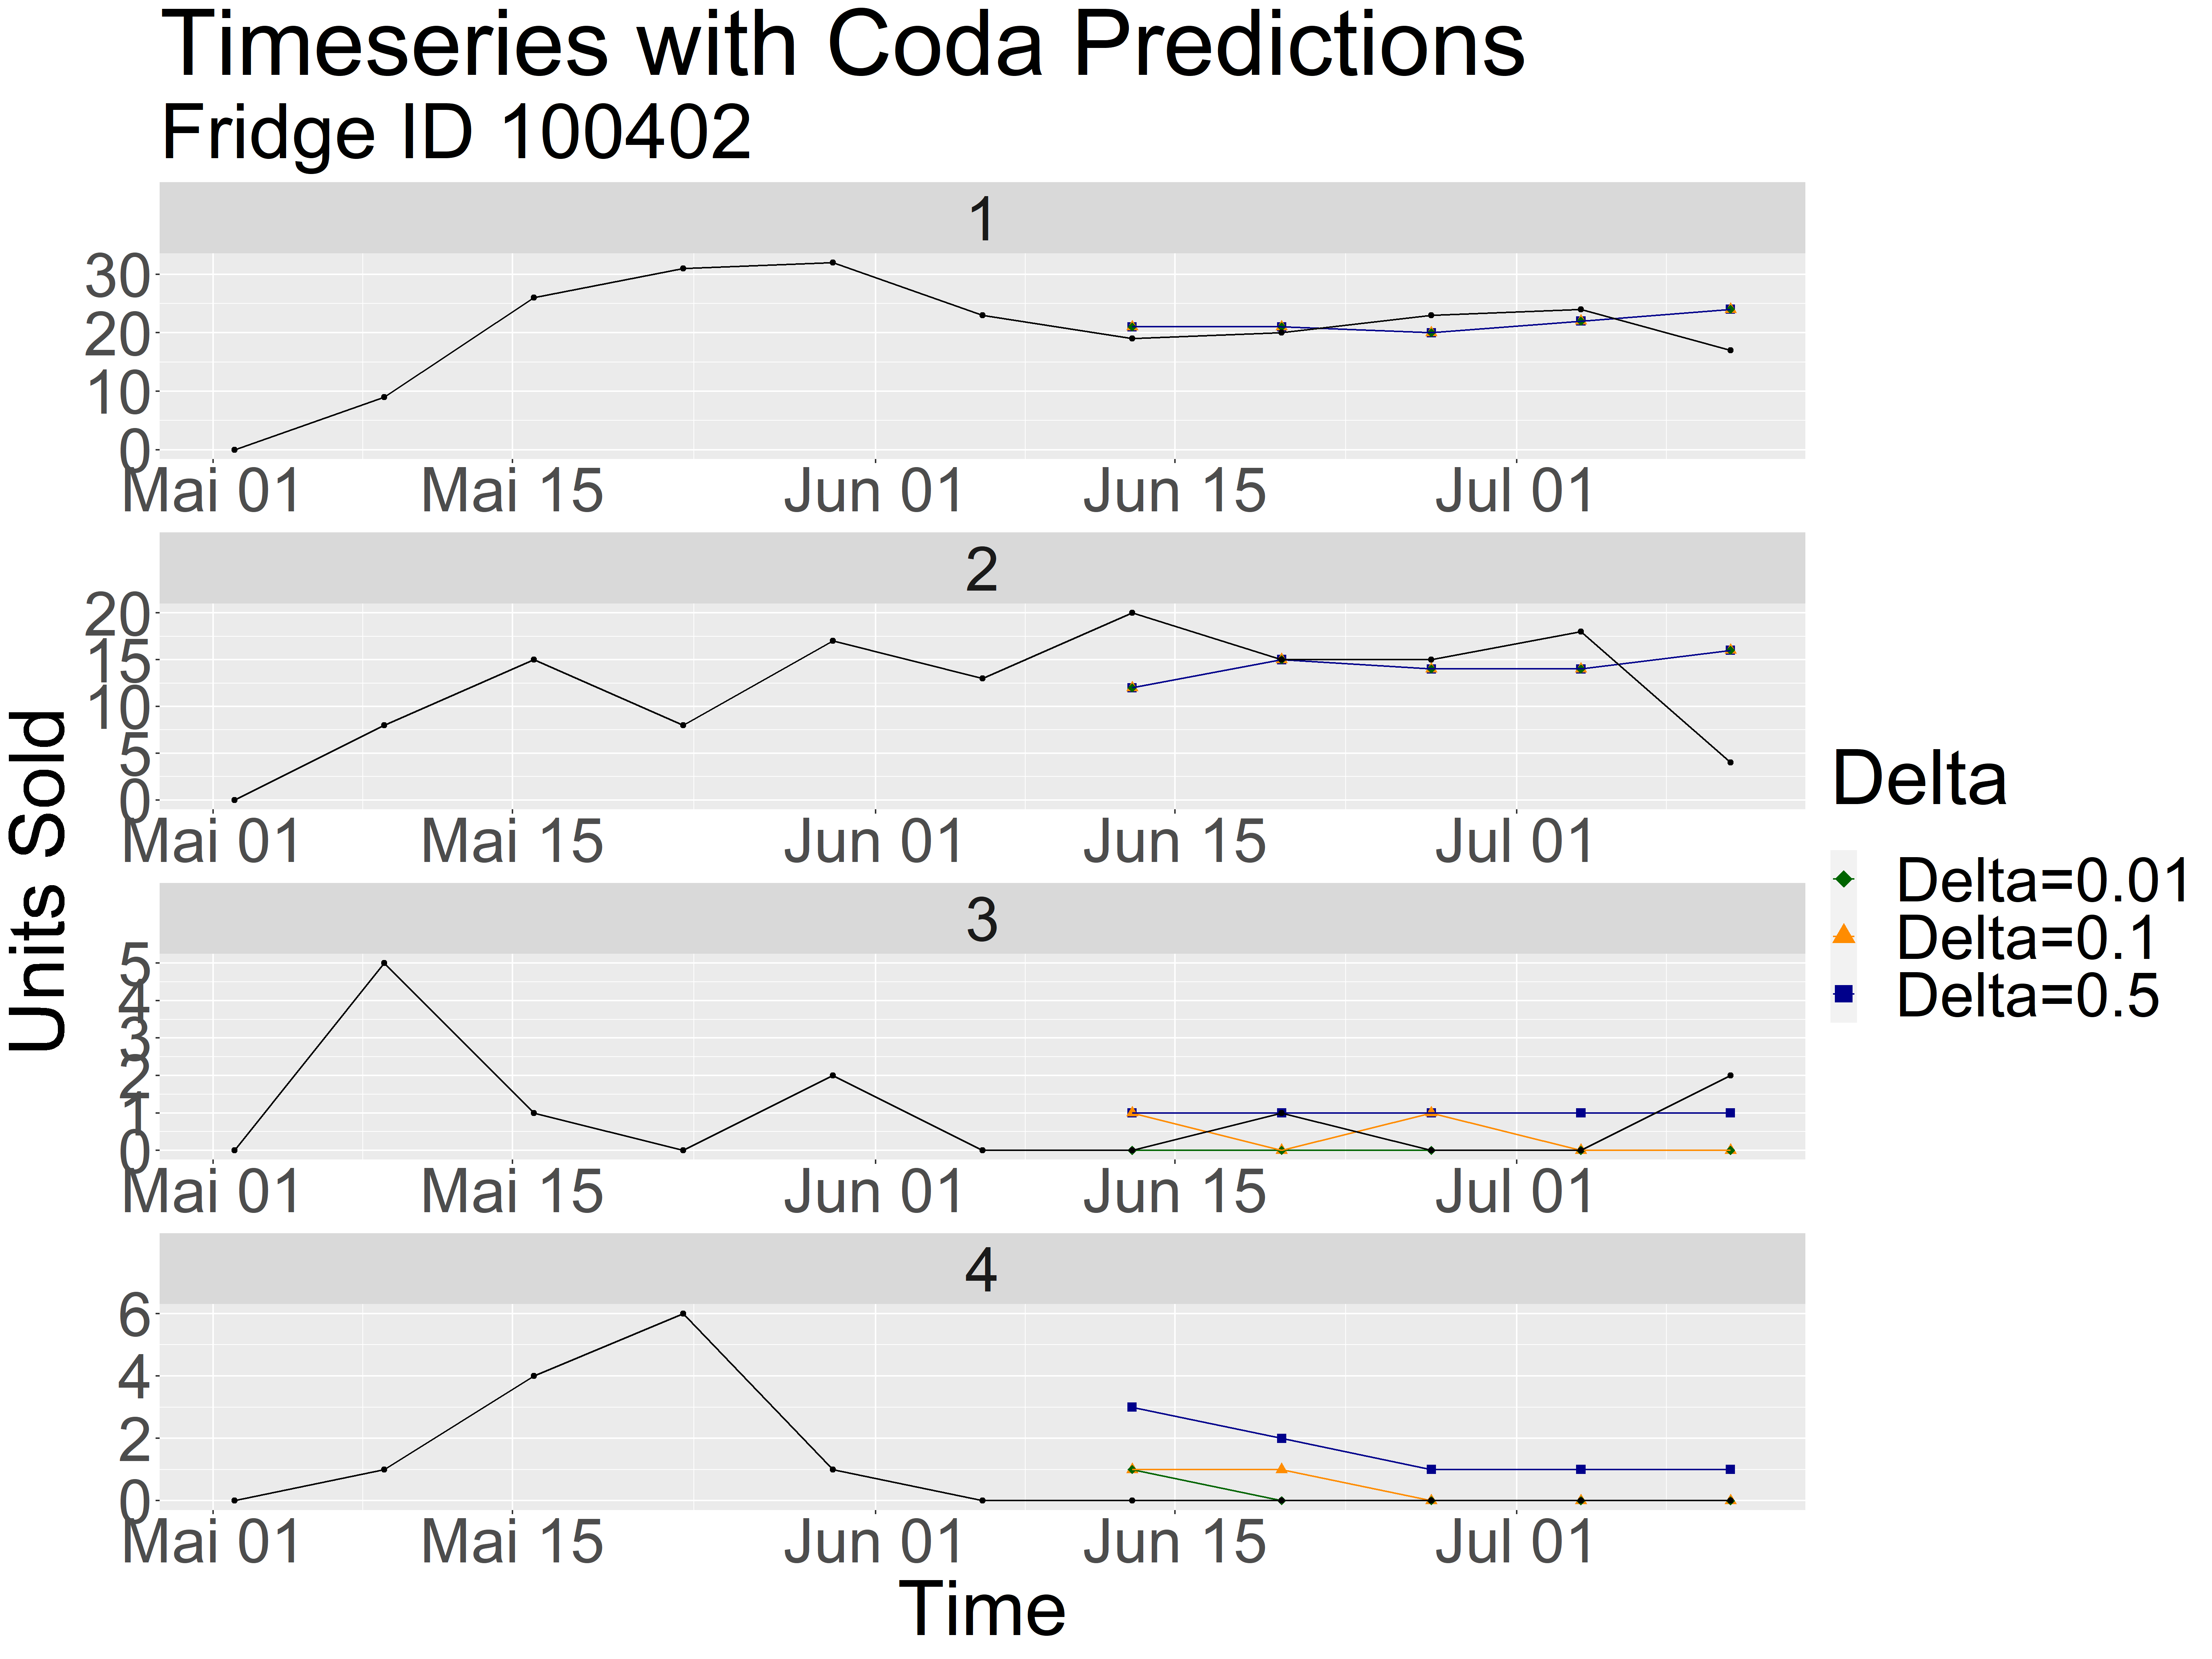
\includegraphics[width=0.80\textwidth]{Graphiken/Coda_Timeseries_VariationdL100402.png}
	\caption{Time series for fridge 100402}
	\label{fig:Coda_Timeseries_ID100402}
\end{figure}

The second highest error for CoDA is for fridge 100403 \ref{fig:Coda_Timeseries_ID100403}. Again, we only have zero values for category 4 and for $\delta=0.5$ CoDA never predicts zero. The same reasoning as above can be used to explain the high error value. 

\begin{figure}[htbp]
	\centering
		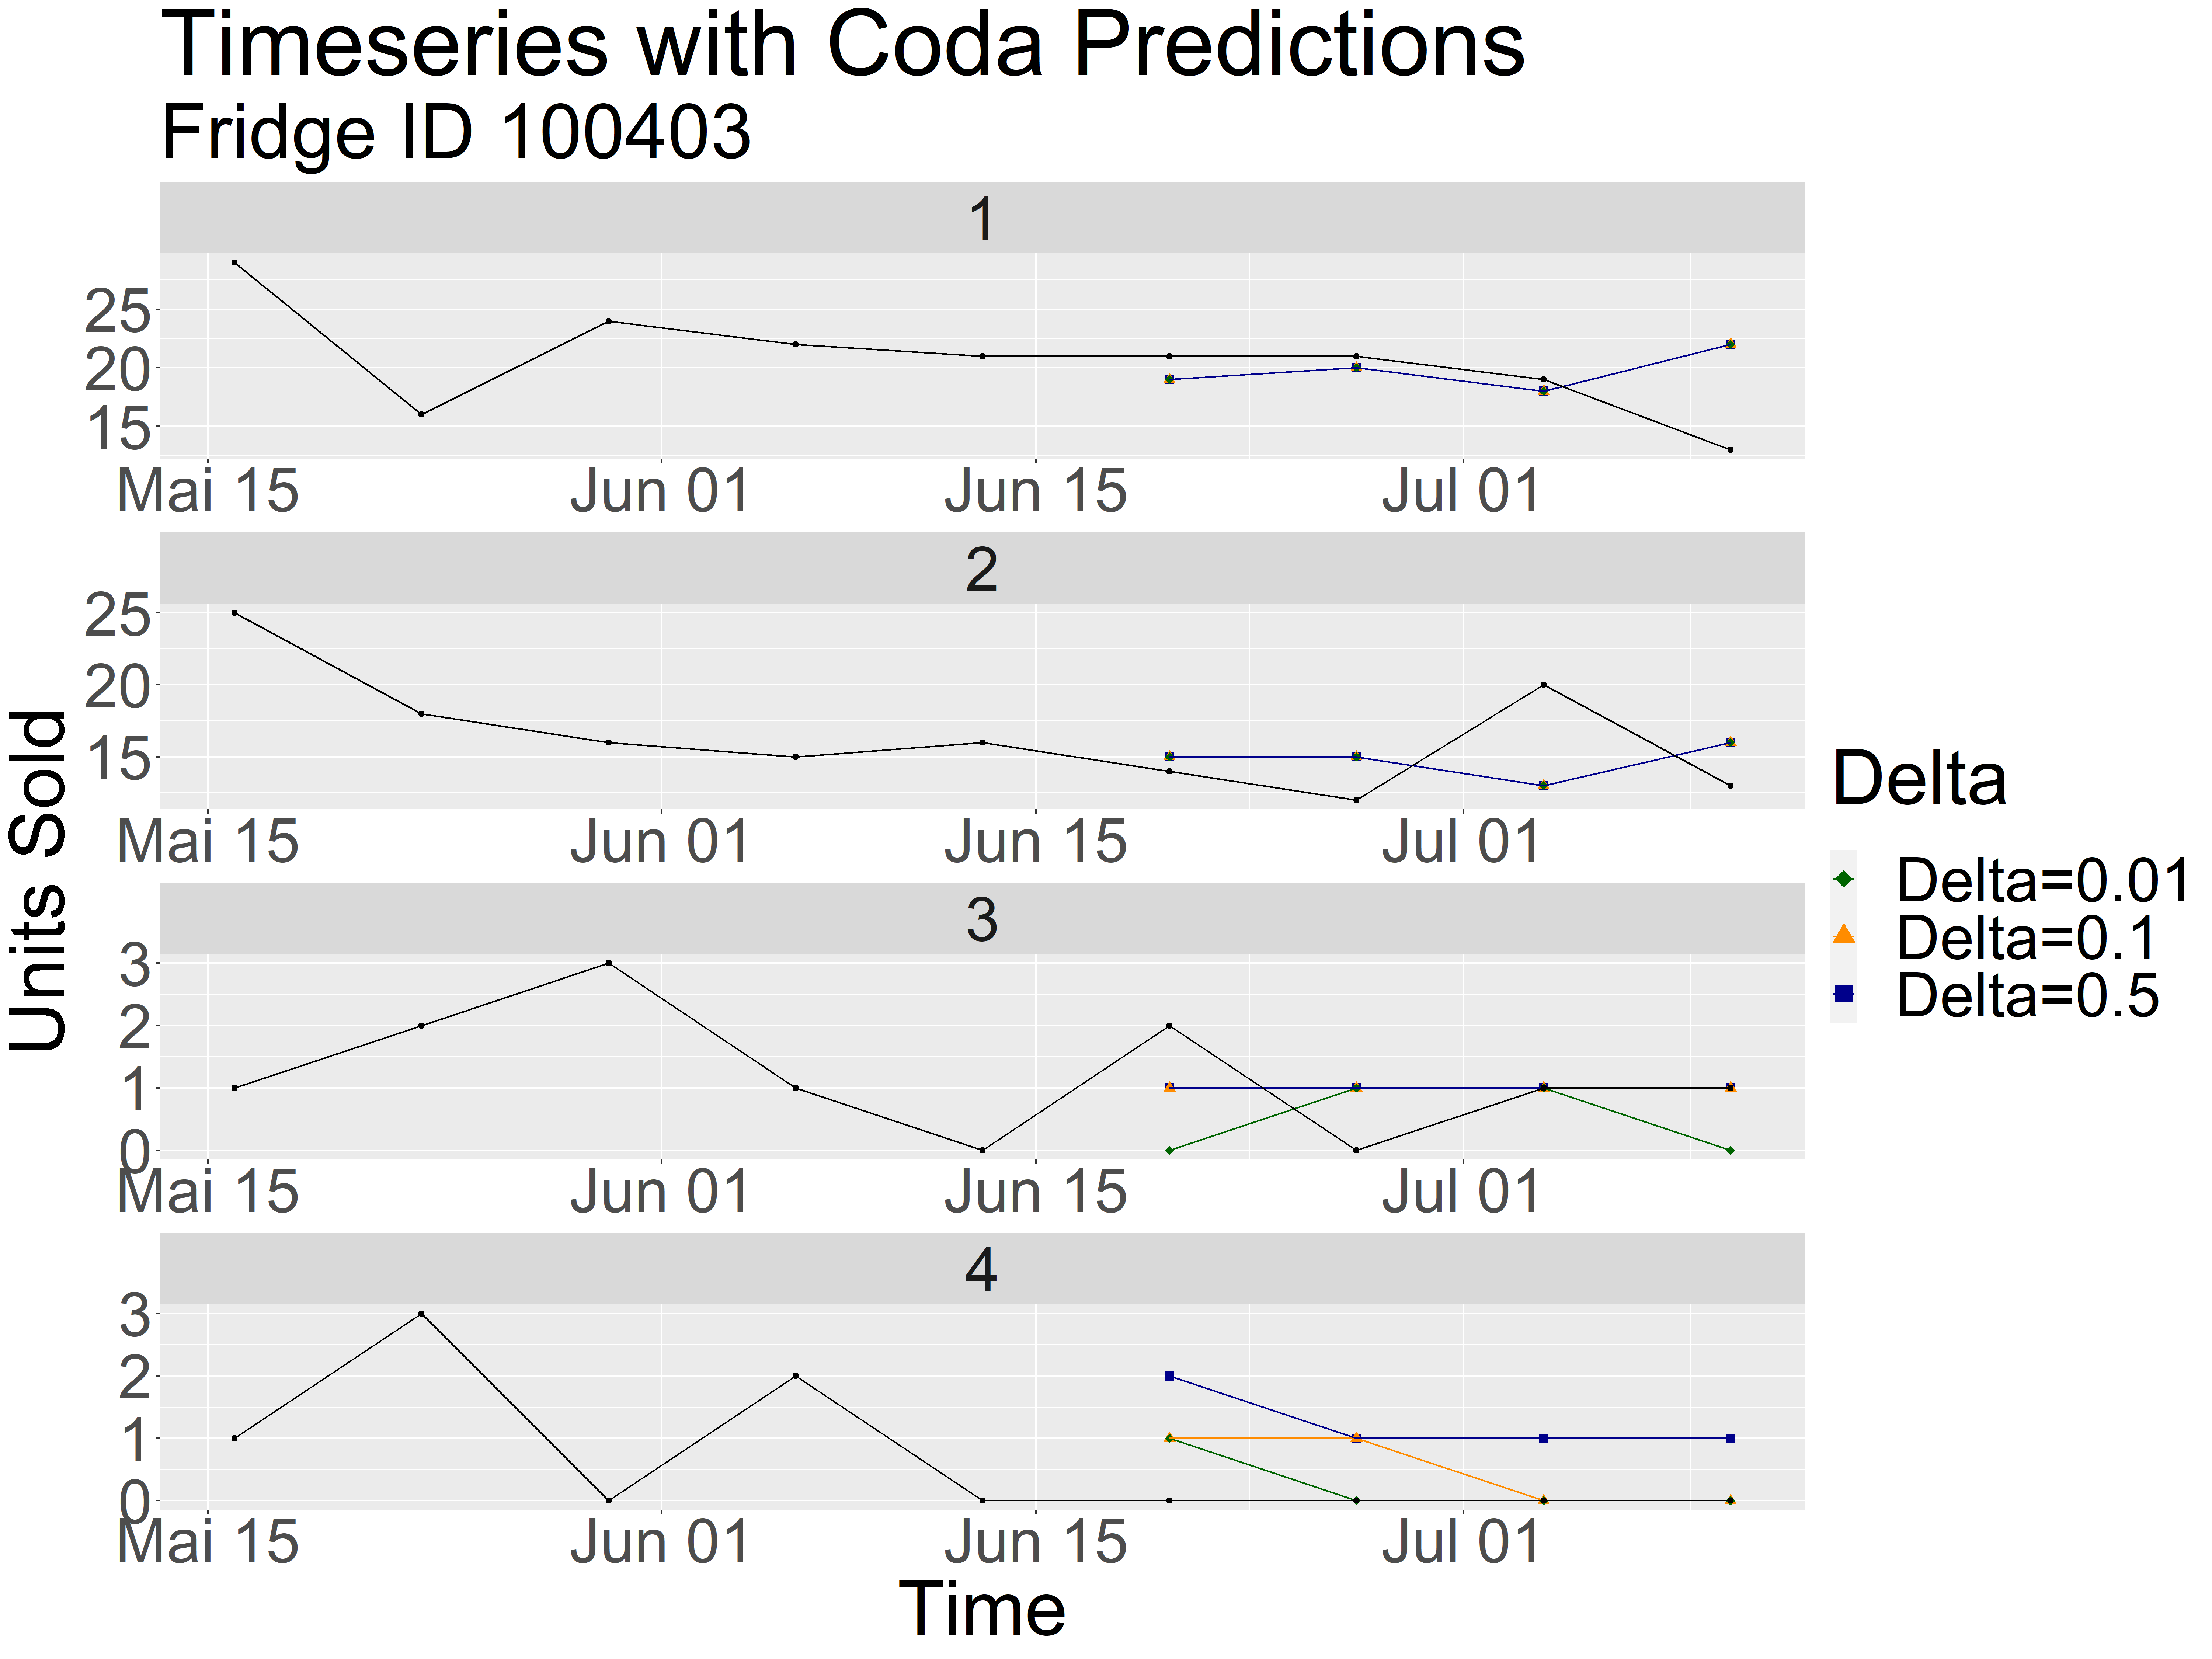
\includegraphics[width=0.80\textwidth]{Graphiken/Coda_Timeseries_VariationdL100403.png}
	\caption{Time series for fridge 100403}
	\label{fig:Coda_Timeseries_ID100403}
\end{figure}

The same thing happens for time series 100191 \ref{fig:Coda_Timeseries_ID100191}. We have an excessive amount of zero values and if $\delta$ is too high, CoDA fails to predict the correct value. 

\begin{figure}[htbp]
	\centering
		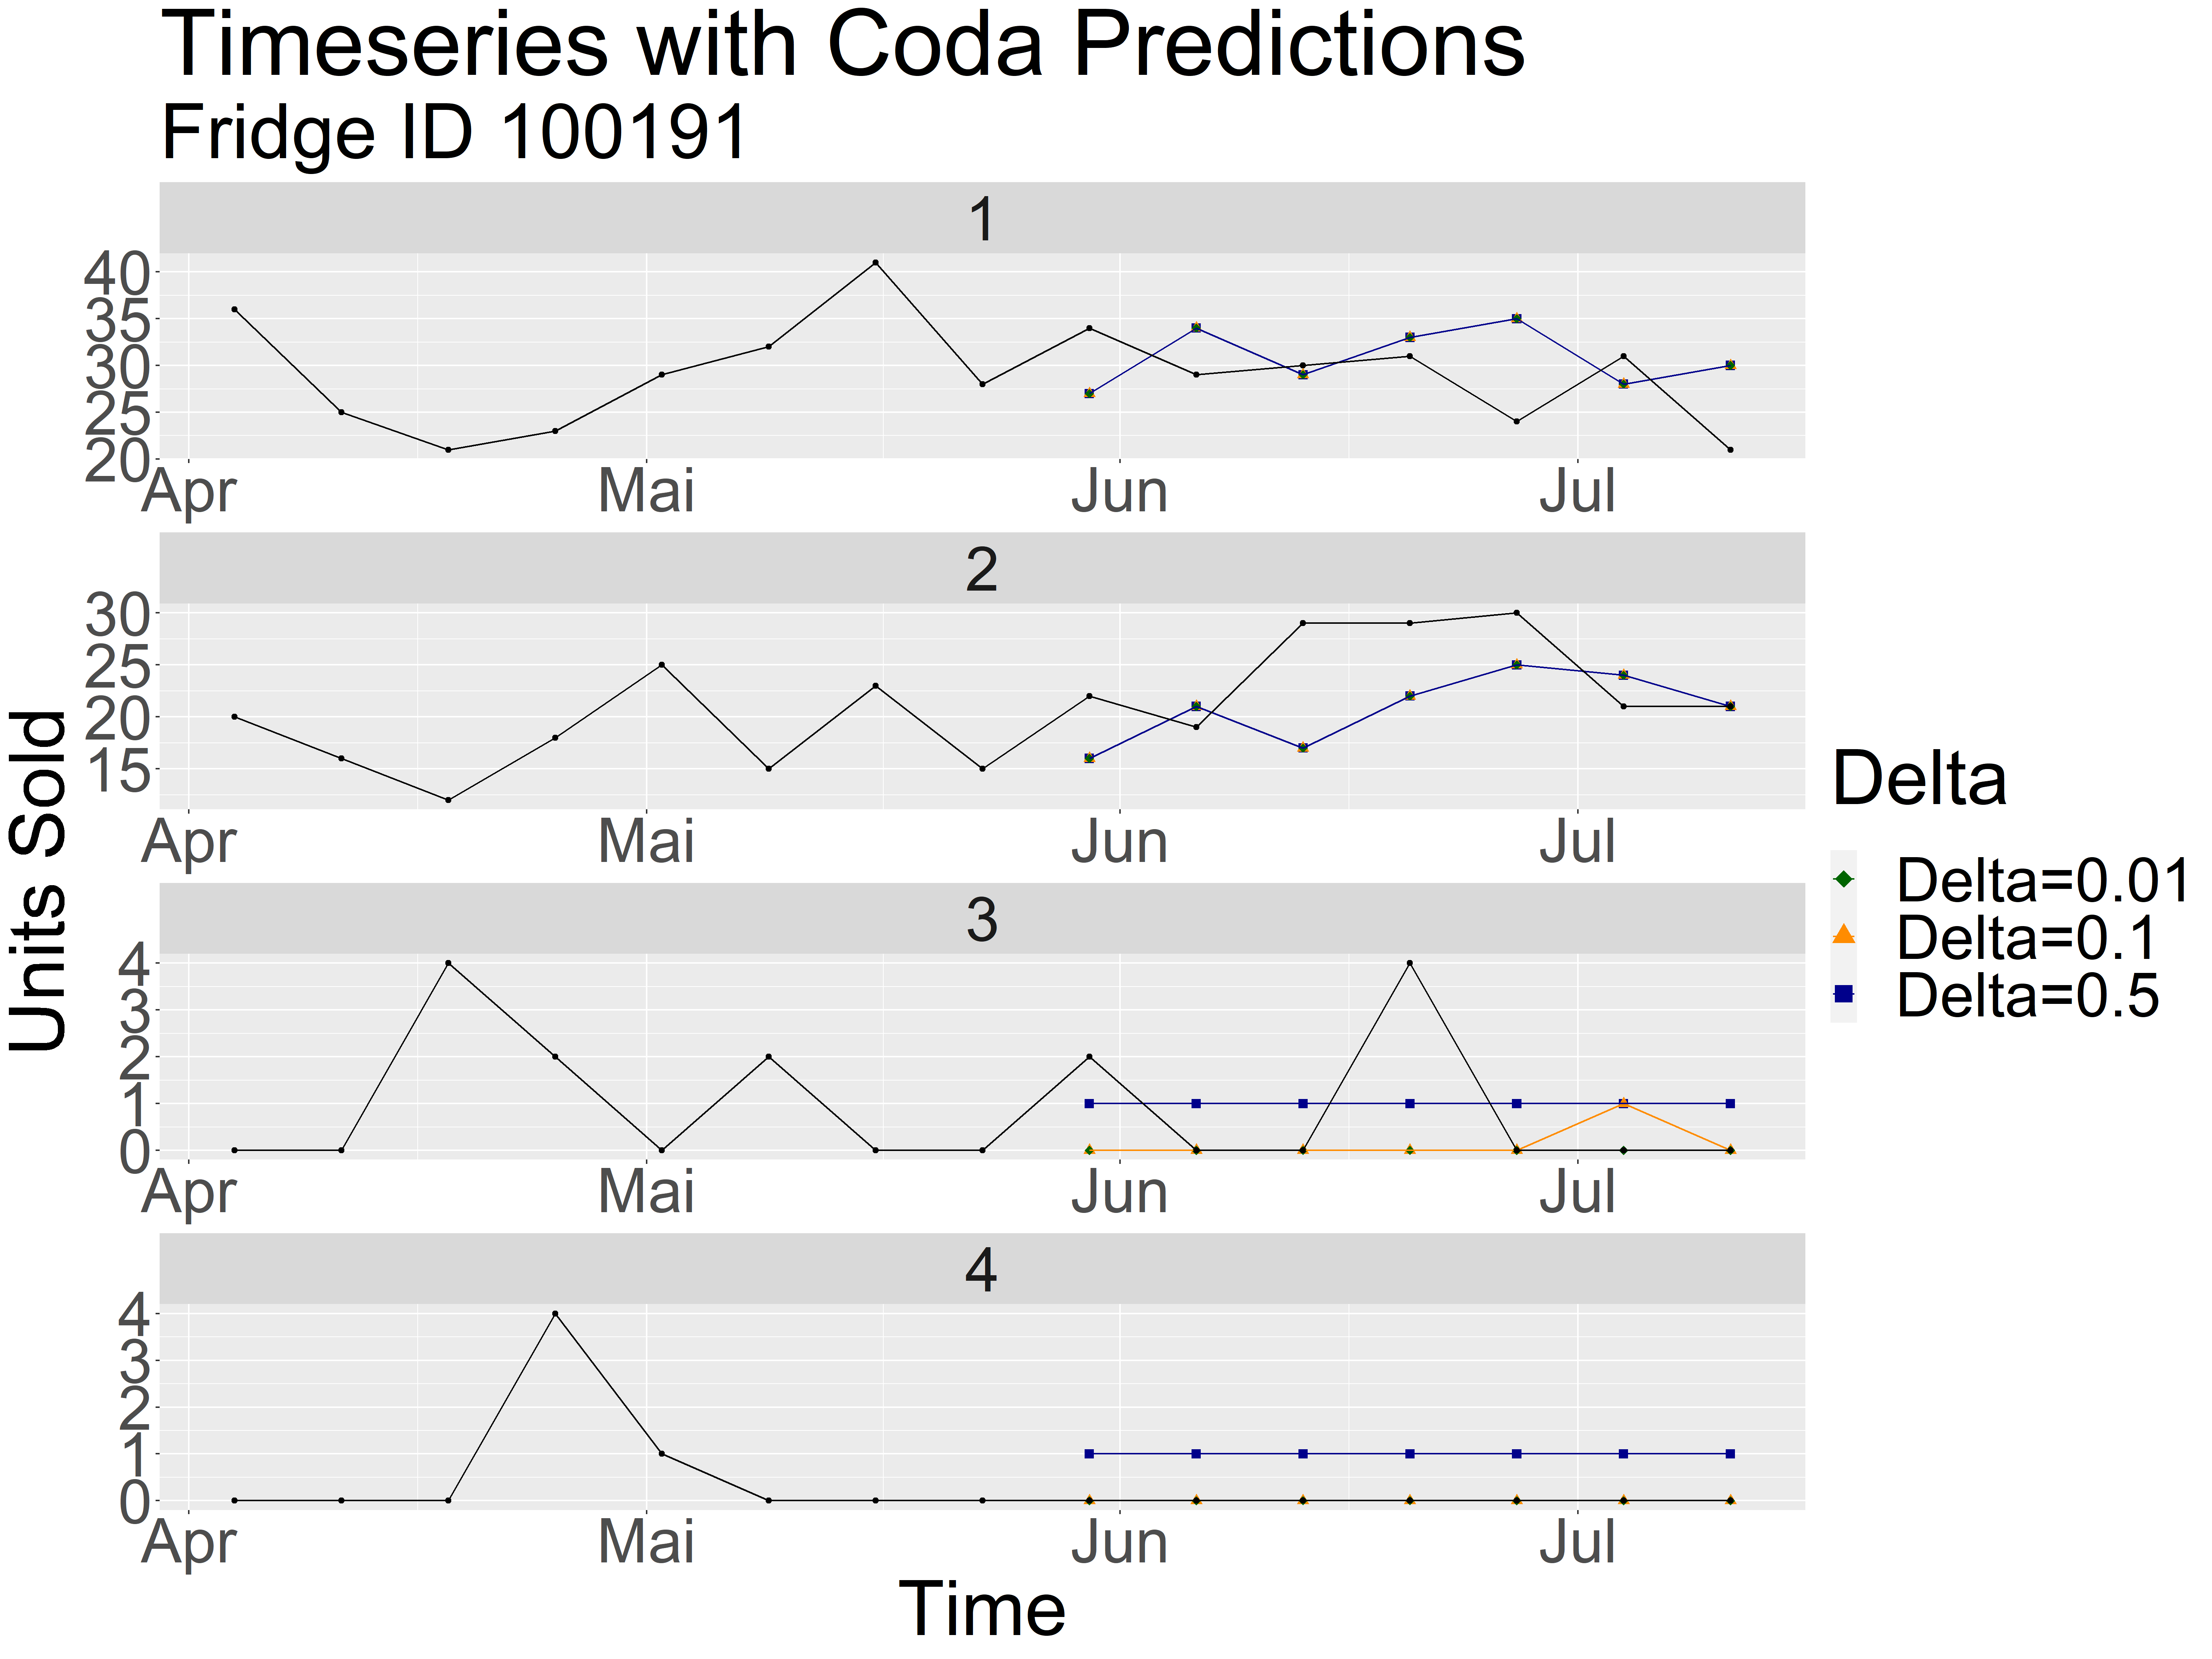
\includegraphics[width=0.80\textwidth]{Graphiken/Coda_Timeseries_VariationdL100191.png}
	\caption{Time series for fridge 100191}
	\label{fig:Coda_Timeseries_ID100191}
\end{figure}

One thing that stands out in these time series is, that for categories 1 and 2, the predicted values are the same for all three values of $\delta$. 

\subsection{$\Tsp$-spaces}
\label{sec: Tspaces results}

Next we compare CoDA for $\Tsp-$Spaces. The results are shown in \ref{fig:Coda T-Spaces Comp1}. It seems that using no $\Tsp-$Spaces result in slightly better results. Especially for shorter time series using no $\Tsp-$Spaces returns better results. This can be seen in figure \ref{fig:Coda T-Spaces Quant}

\begin{figure}[htb!]
\centering
\begin{subfigure}[b]{0.45\textwidth}
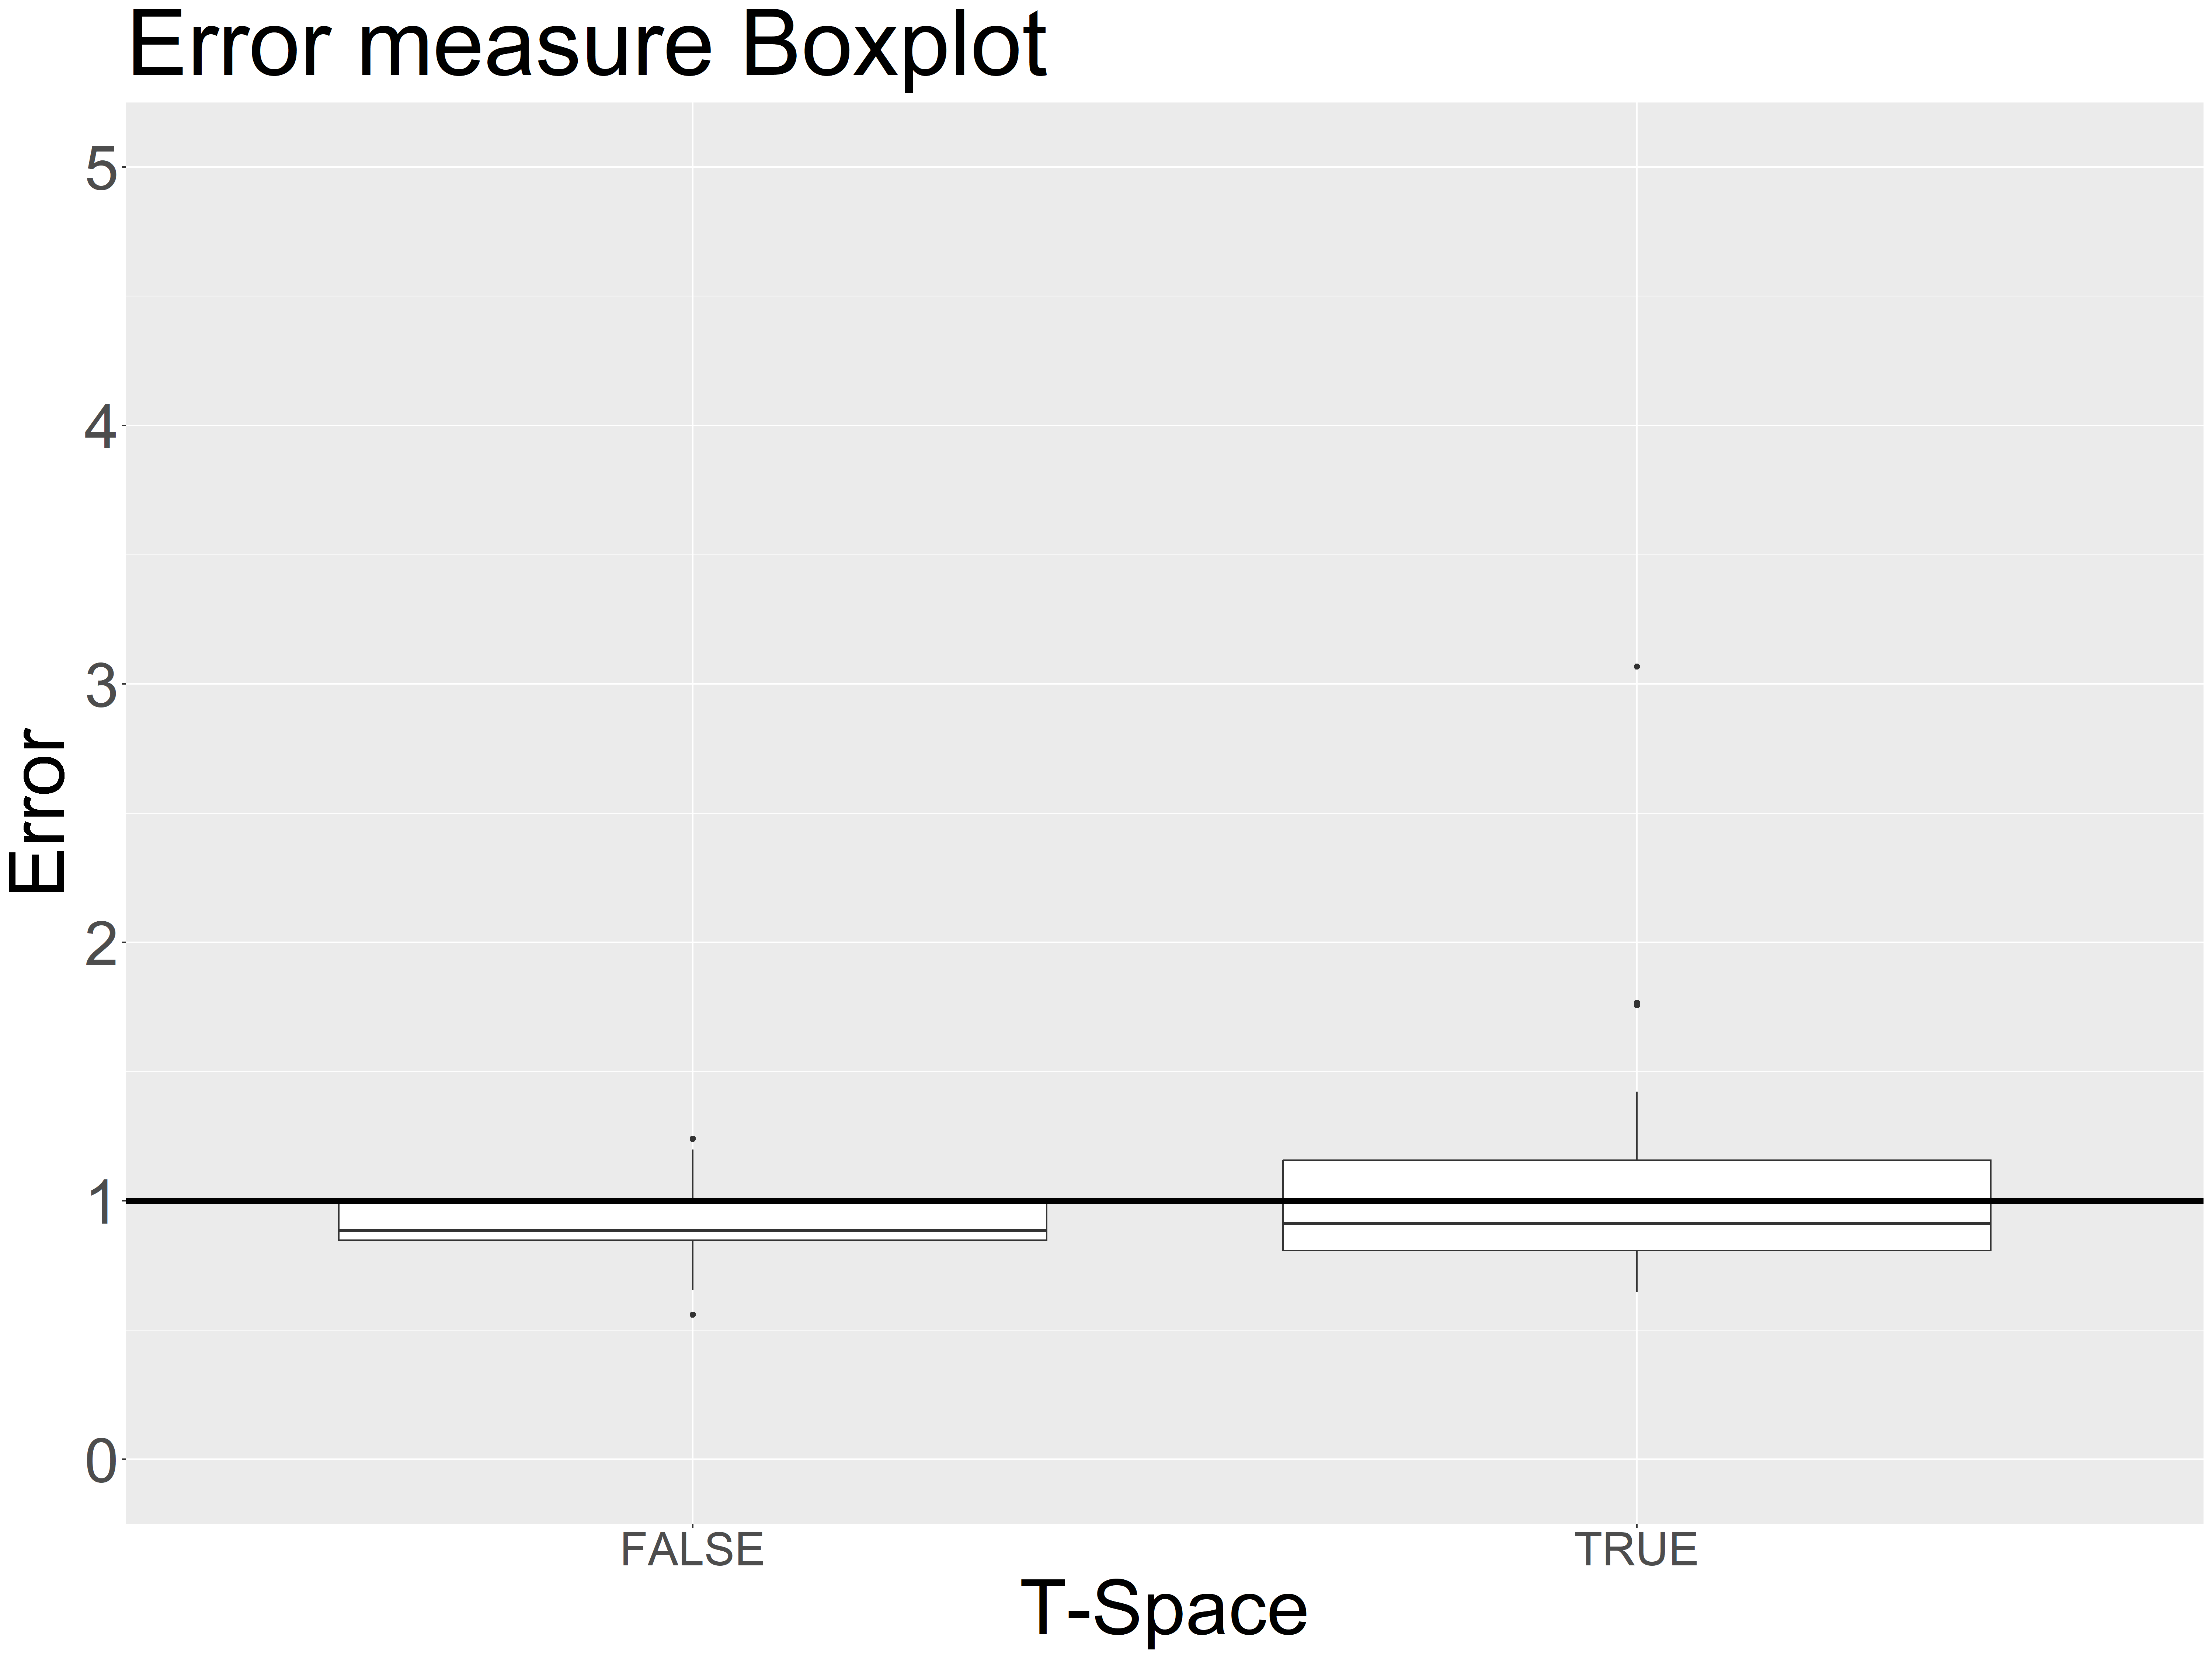
\includegraphics[width=\textwidth]{ErrorMeasureCoDA_Box_all__Variation_tSpace.png}
\caption{Boxplot for $\Tsp-$Spaces}
\label{fig:Coda T-Spaces Box}
\end{subfigure}
\hfill
\begin{subfigure}[b]{0.45\textwidth}
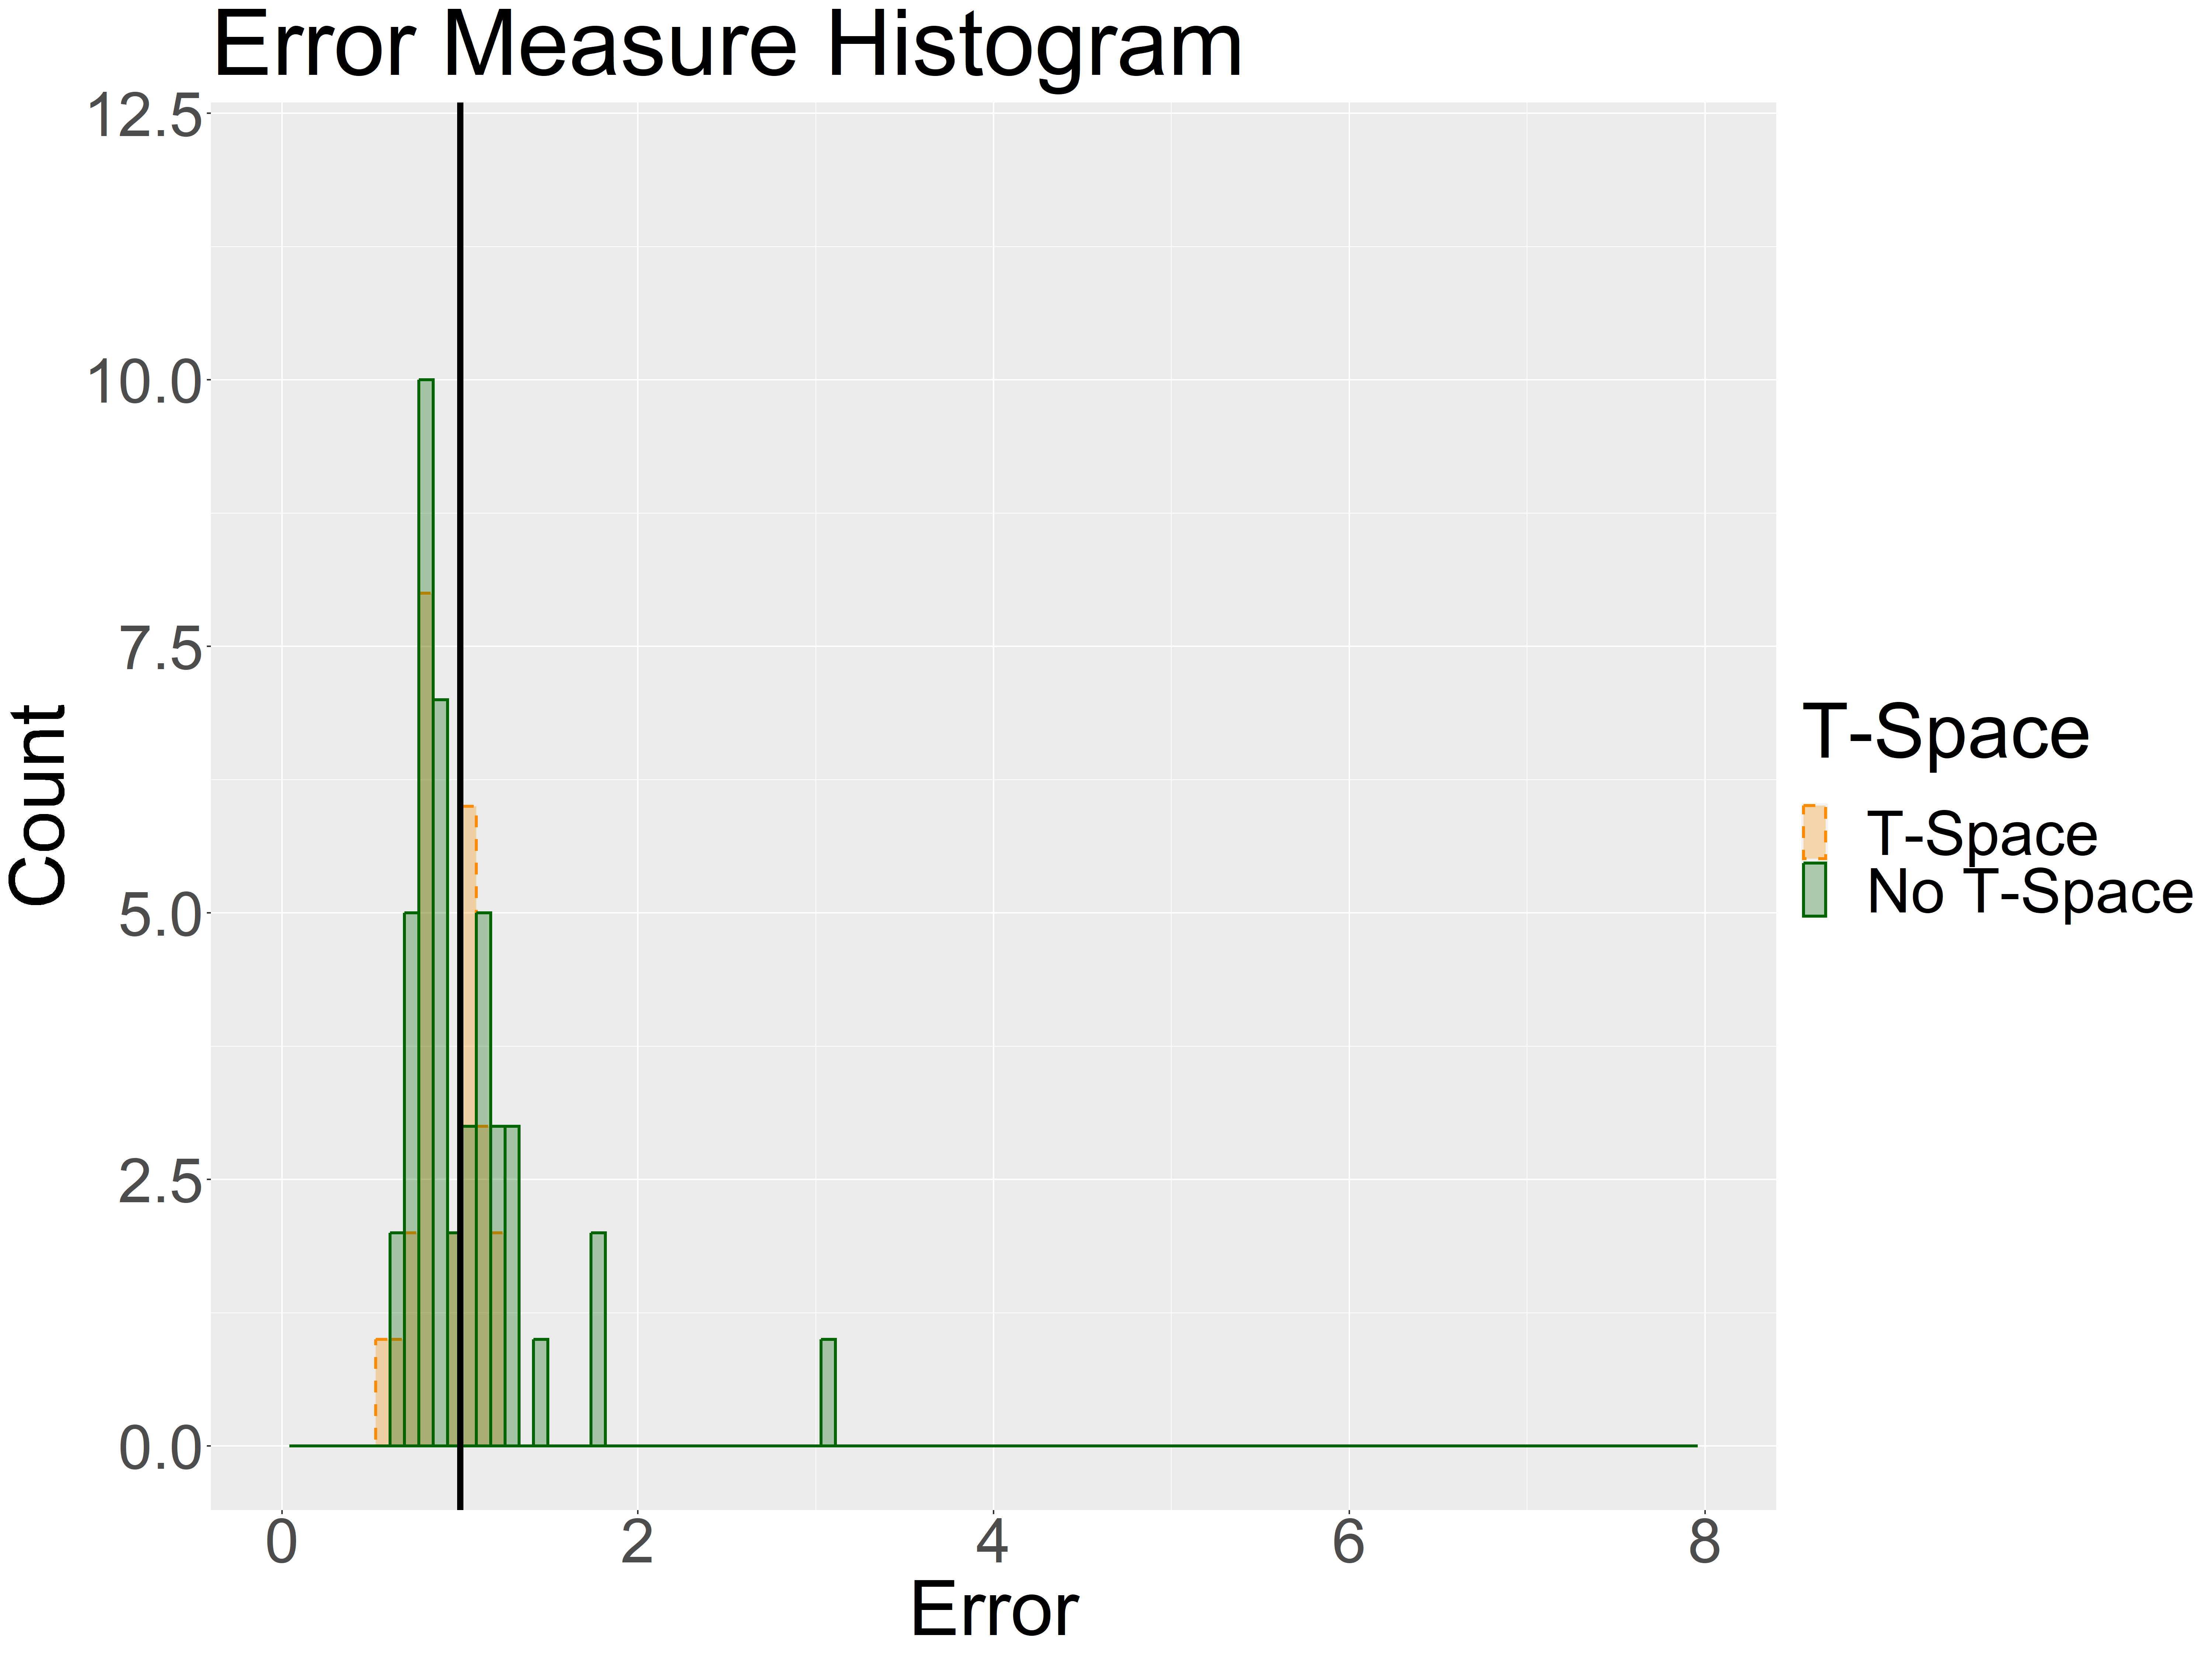
\includegraphics[width=\textwidth]{ErrorMeasureCoDA_Histogram_all__Variation_tSpace.png}
\caption{Histogram for $\Tsp-$Spaces}
\label{fig:Coda T-Spaces Hist}
\end{subfigure}
\hfill
\begin{subfigure}[b]{0.8\textwidth}
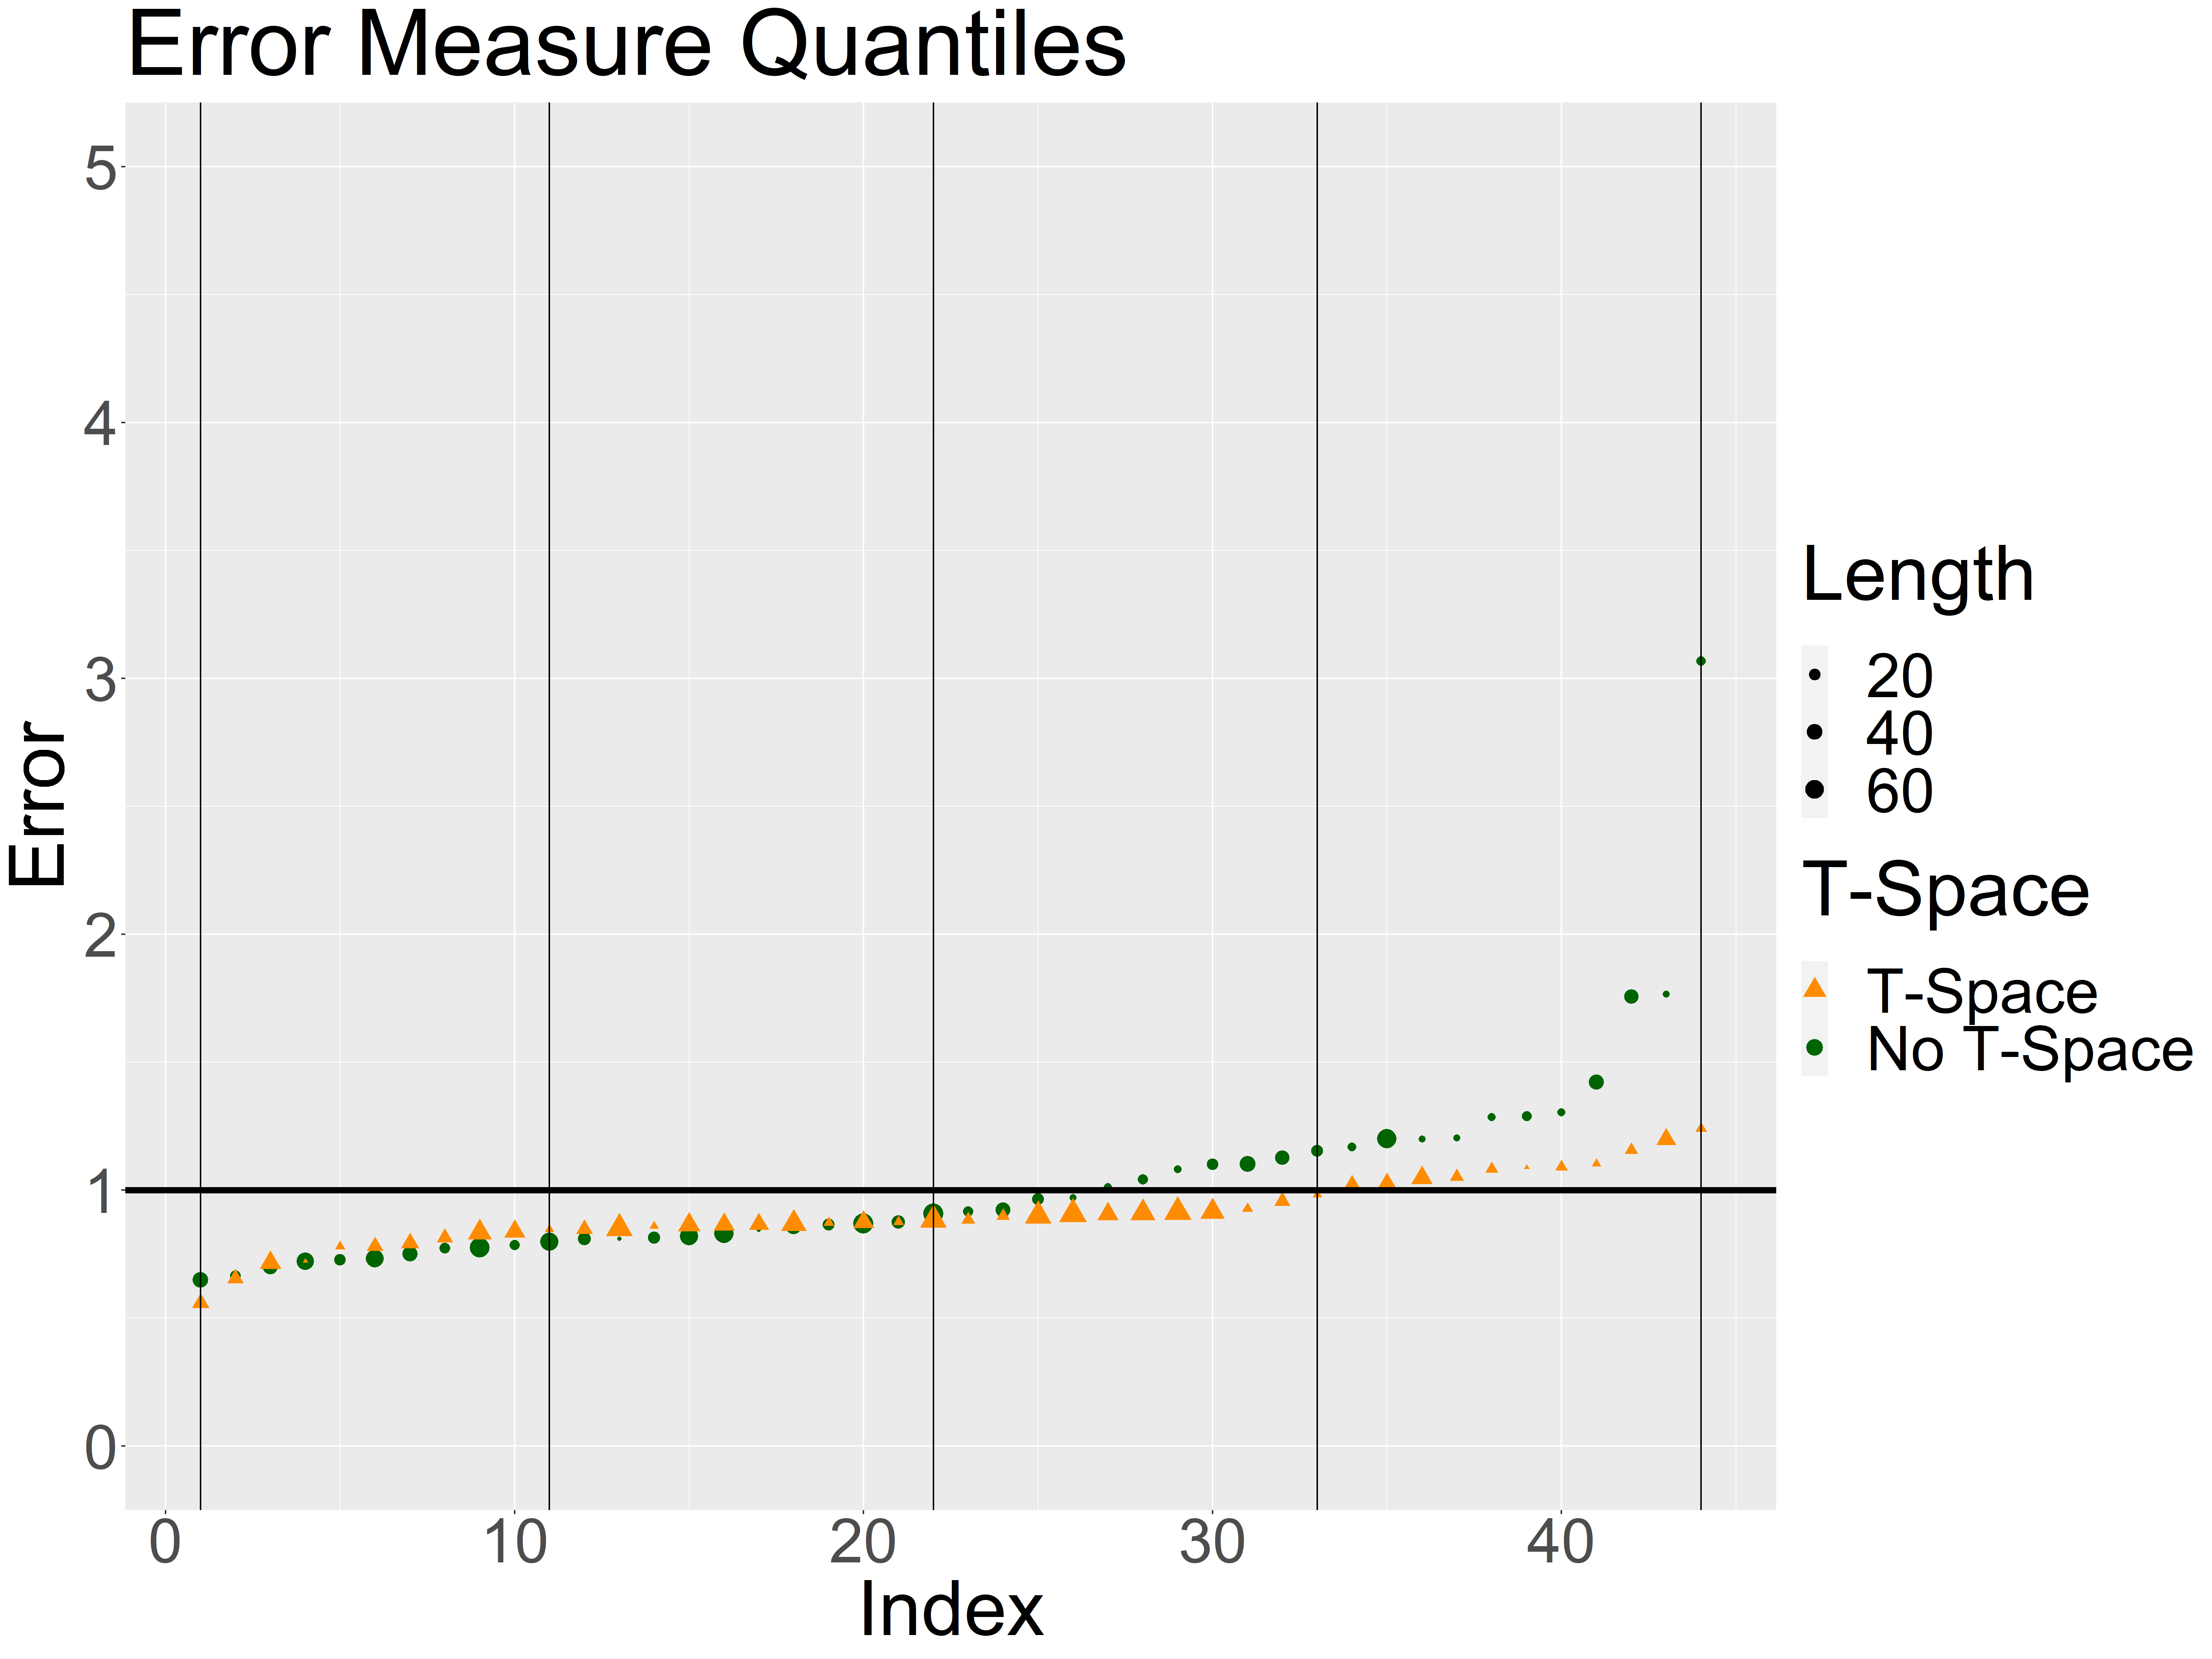
\includegraphics[width=\textwidth]{ErrorMeasureCoDA_Quant_all__Variation_tSpace.png}
\caption{Quantiles for $\Tsp-$Spaces}
\label{fig:Coda T-Spaces Quant}
\end{subfigure}
\caption{Comparison of CoDA with and without $\Tsp-$Spaces}
\label{fig:Coda T-Spaces Comp1}
\end{figure}

To further investigate the reason of this difference in performance, we picked out the two time series with the highest error. The fridge with the highest error had Id 100321. Its time series can be seen in \ref{fig:Coda_Timeseries_VariationtSpace100321}. As we can seen, CoDA with $\Tsp$-Spaces performs worse for category 1 and 2. However, the time series is also short by nature with only 14 recorded points in time.  

\begin{figure}[htbp]
	\centering
		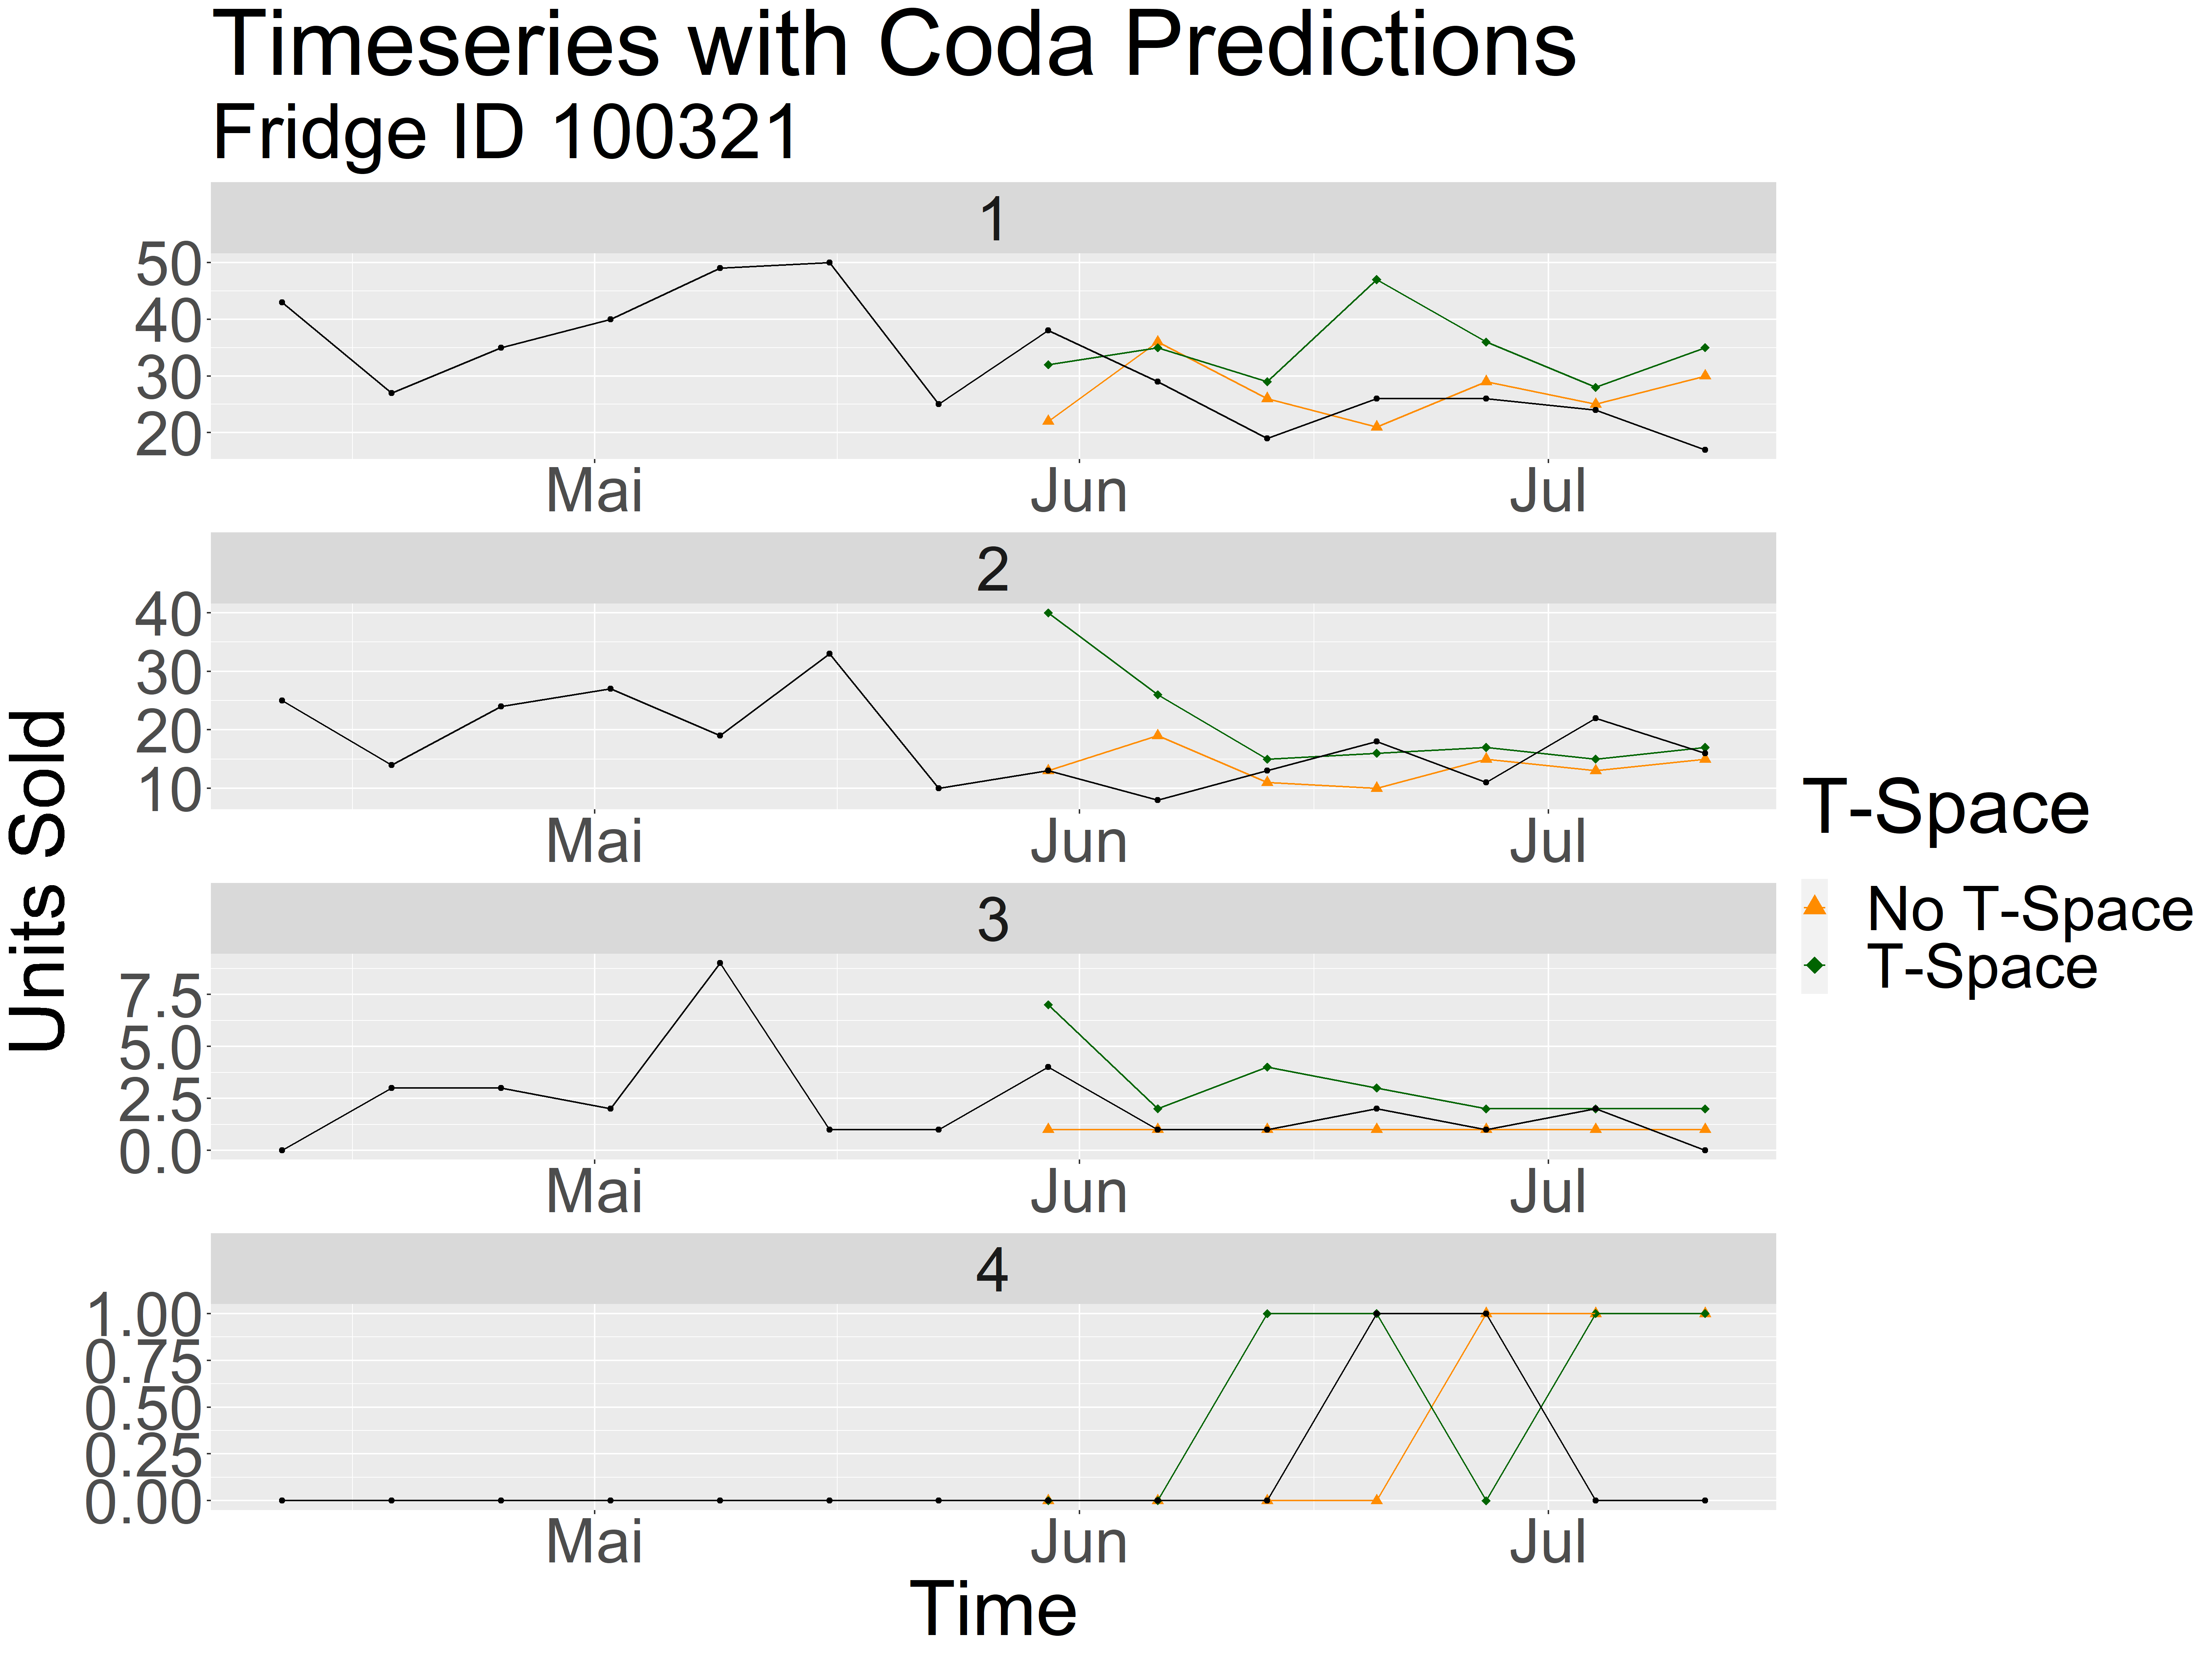
\includegraphics[width=0.80\textwidth]{Graphiken/Coda_Timeseries_VariationtSpace100321.png}
	\caption{Time series of fridge 100321}
	\label{fig:Coda_Timeseries_VariationtSpace100321}
\end{figure}

The second highest error measure has fridge 20 \ref{fig:Coda_Timeseries_VariationtSpace20}. Again, the problem lies in category 1 and 2. Especially for category 1, CoDA with $\Tsp$-Space seems to continuously underestimate the true values. For category 3 and 4, both settings have very similar results.

\begin{figure}[htbp]
	\centering
		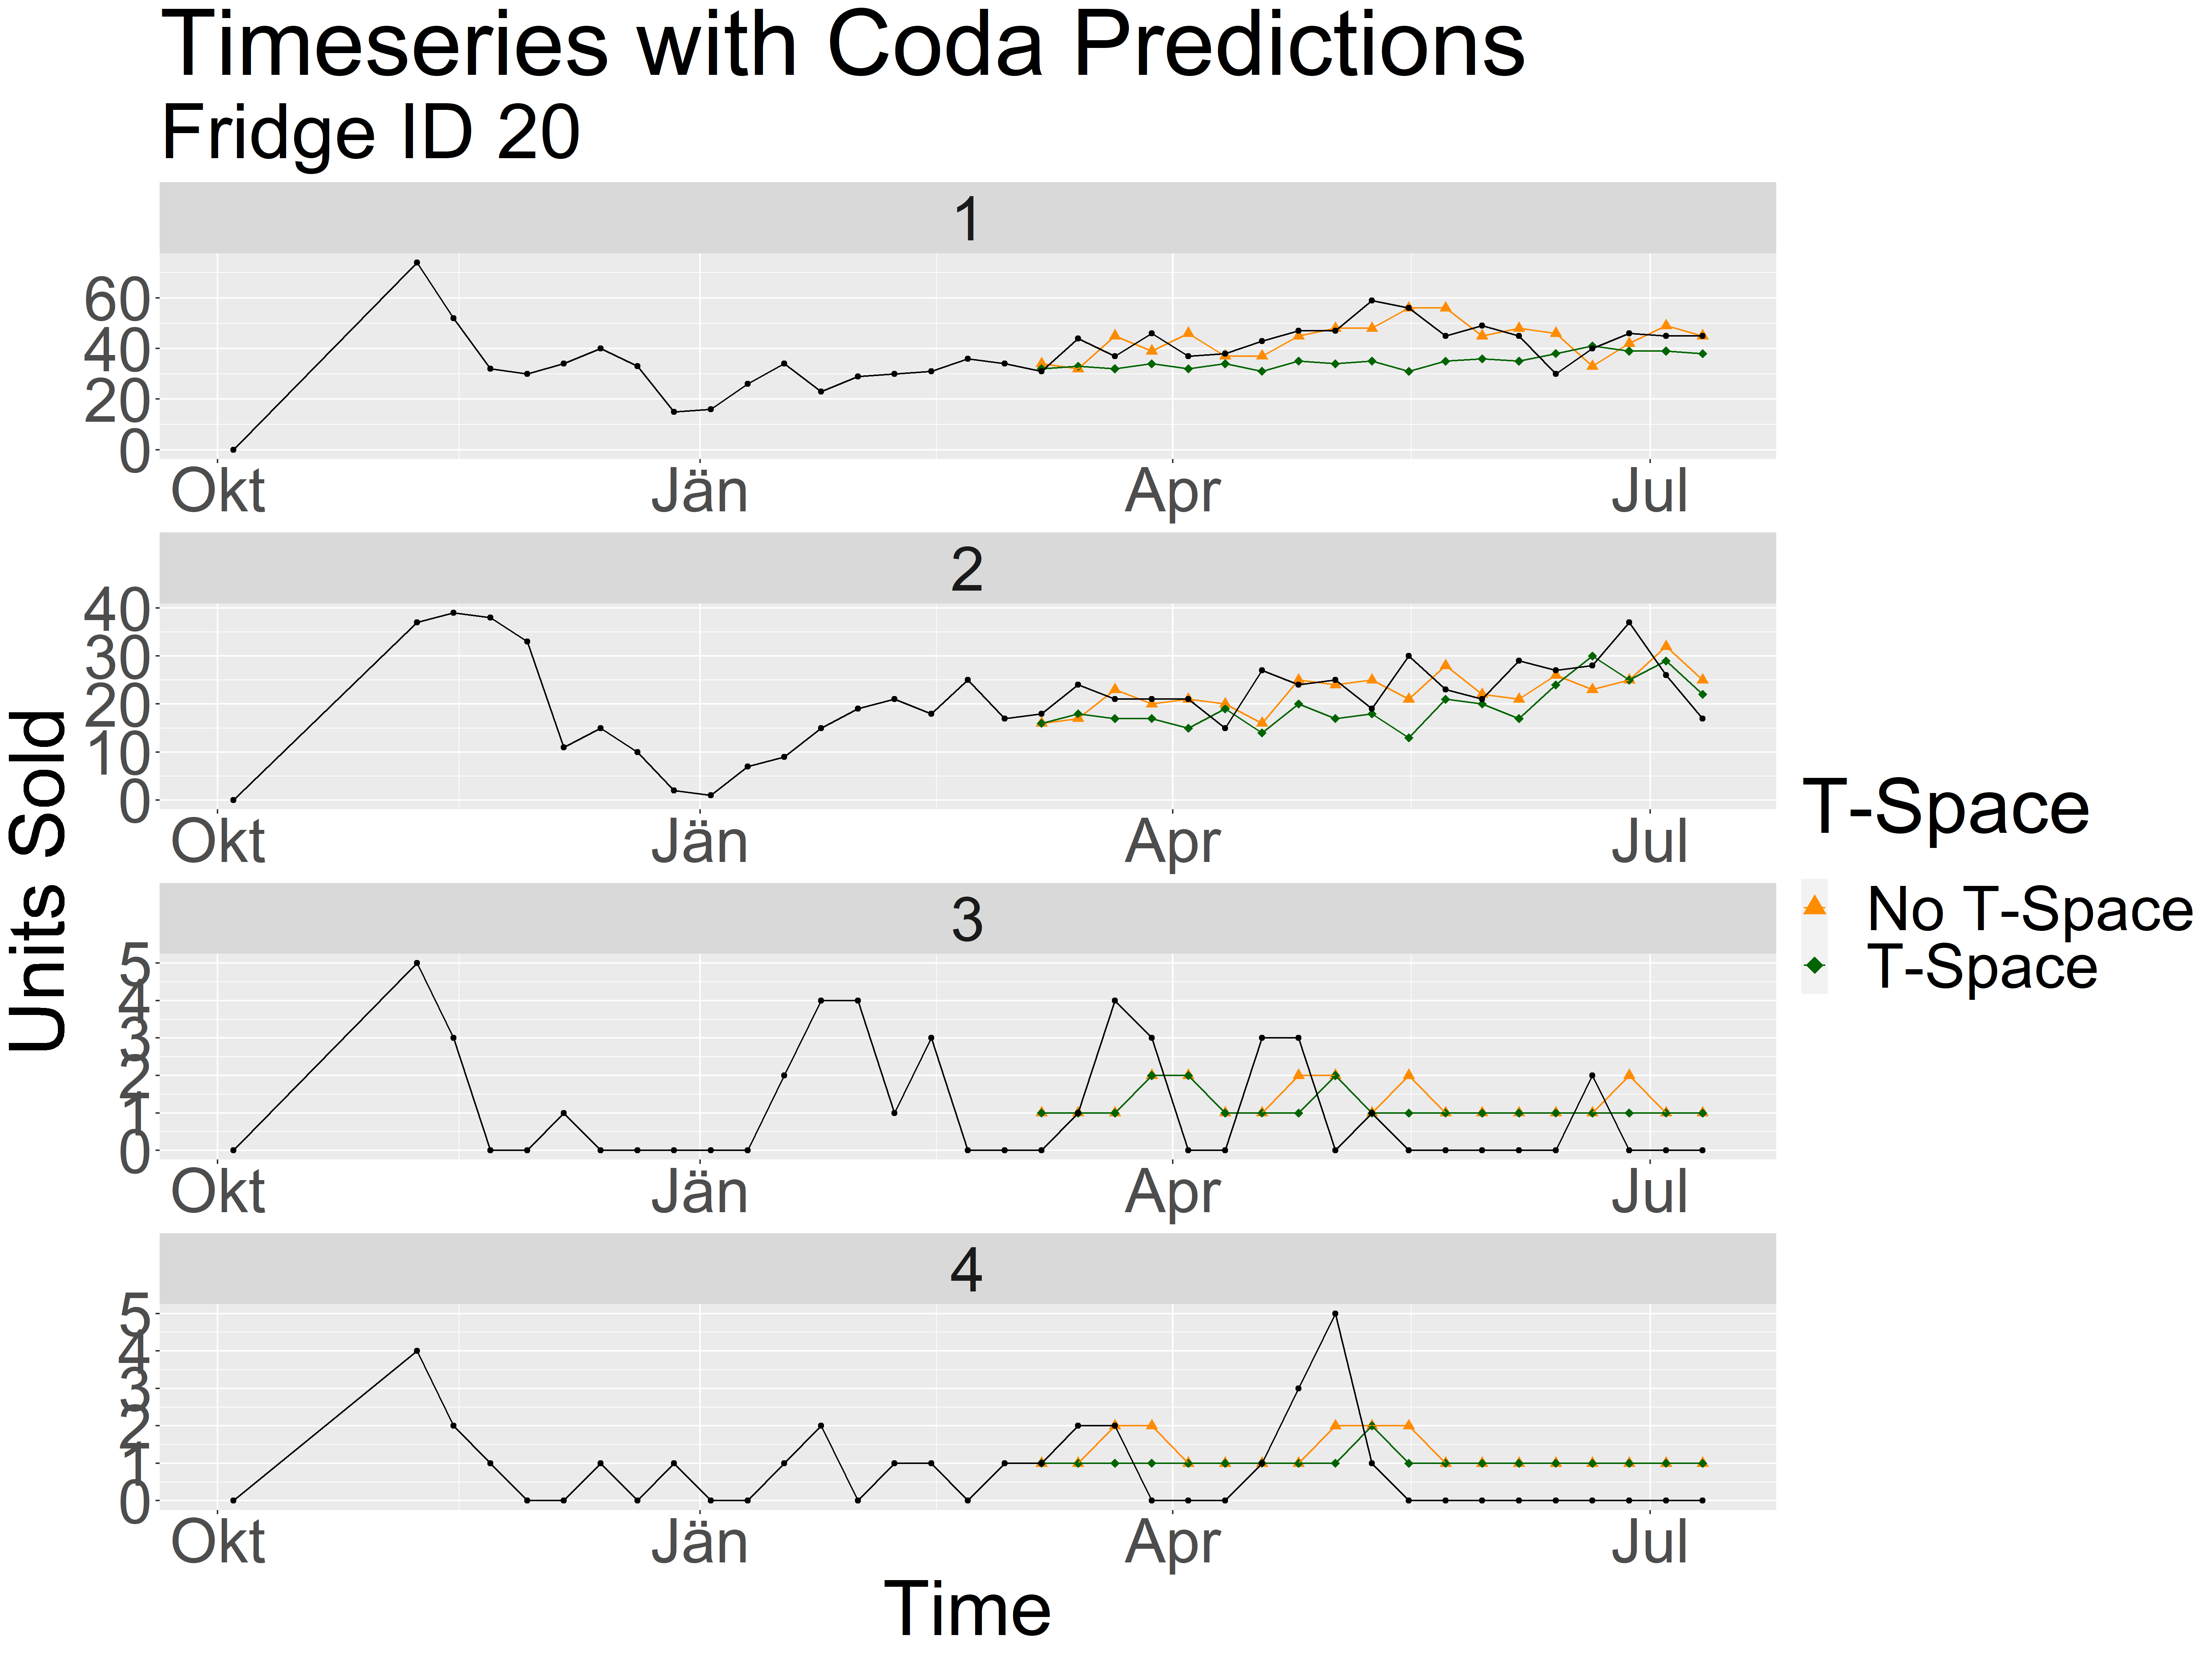
\includegraphics[width=0.80\textwidth]{Graphiken/Coda_Timeseries_VariationtSpace20.png}
	\caption{Time series of fridge 20}
	\label{fig:Coda_Timeseries_VariationtSpace20}
\end{figure}

\subsection{One-vs-All method}
\label{sec: One-vs-All}

Now we analyse the one-vs-all method. Figure \ref{fig:Coda One-vs-All Comp1} shows the results. We can clearly seen, that the one-vs-all method performs better over all time series. This difference is highlighted in figure \ref{fig:Coda One-vs-All Quant}. 

\begin{figure}[htb!]
\centering
\begin{subfigure}[b]{0.45\textwidth}
\includegraphics[width=\textwidth]{ErrorMeasureCoDA_Box_all__Variation_oneVSAll.png}
\caption{Boxplot for One-vs-All}
\label{fig:Coda One-vs-All Box}
\end{subfigure}
\hfill
\begin{subfigure}[b]{0.45\textwidth}
\includegraphics[width=\textwidth]{ErrorMeasureCoDA_Histogram_all__Variation_oneVSAll.png}
\caption{Histogram for One-vs-All}
\label{fig:Coda One-vs-All Hist}
\end{subfigure}
\hfill
\begin{subfigure}[b]{0.8\textwidth}
\includegraphics[width=\textwidth]{ErrorMeasureCoDA_Quant_all__Variation_oneVSAll.png}
\caption{Quantiles for One-vs-All}
\label{fig:Coda One-vs-All Quant}
\end{subfigure}
\caption{Comparison of CoDA with and without One-vs-All}
\label{fig:Coda One-vs-All Comp1}
\end{figure}


















%%%%%%%%%%%%%%%%%%%%%%%%%%%%%%%%%%%%%%%%%%%%%%%%%%%%%%%%%%%%%
%% LITERATUR UND ANDERE VERZEICHNISSE
%%%%%%%%%%%%%%%%%%%%%%%%%%%%%%%%%%%%%%%%%%%%%%%%%%%%%%%%%%%%%

\chapter{Conclusion}
\label{sec: Conclusion}
In this thesis, we compare multiple models for multivariate count data time series with an excessive amount of zeros with the goal of finding the optimal model for predicting future values. A special focus lies in the integer-valued generalized autoregressive conditional heteroskedasticity model of order (p,q) (INGARCH(p,q) model) and the compositional data analysis (CoDA) model. The other models include a zero-inflated model (ZIM) and an integer-valued autoregressive model of order p (INAR(p) model). Since this thesis is carried out as part of a bigger project at the Technical University of Austria in cooperation with Schrankerl GmbH, we were able to test our models on real world data and compare them with the model currently in use. 

The current model used for forecasting is the naive random walk model. While in general, all tested models outperform the current model and deliver a similar output, they come with their respective advantages and disadvantages.

The INGARCH model considers the discrete nature of our data, but ignores both, the multivariate structure of it and the appearance of an unusual amount of zeros. While there exists a multivariate version of the INGARCH model, to our knowledge, there is no software implementation in R. The fitting of a multivariate INGARCH model and assuming the data to be ZIP distributed, can be grounds for further investigations. % In addition, the INGARCH model assumes the data to be Poisson or Negative Binomial distributed and hence does not accommodate to the excessive amount of zeros.

The CoDA model fits a multivariate model and sees our data as a compositional time series. While it also neglects the fact that we have integer-valued data, the biggest issue with CoDa is, that the data must not include zeros. While there exist various methods to handle zero values as presented in Section \ref{sec: Zero-Handling}, the handling of essential zeros, which is what we have, still remains problematic. We opt for the suggested data amalgamation and the simple replacement strategy because of their simplicity but a better way of handling zeros could be worth future research. 

The INAR model has similar assumptions as the INGARCH model. It accounts for the discrete nature of our data, but neglects its multivariate structure and the amount of excessive zeros. The excessive zeros seem to be troublesome for the INAR model in general, since it performs the worst out of all models for time series with many zeros. 

The zero-inflated model is an intriguing model. It considers both, the excessive amounts of zeros, and the discrete nature of our data and only ignores the multivariate structure of it. However, while we do have an excessive amount of zeros, we do not necessarily have zeros in every category of the time series and especially not if we only use parts of them. But since the zero-inflated model needs to have at least one zero in the sample, it cannot be fit on samples with no zeros present. This restricts us to fit the ZIM only on the categories with the most zeros present. 

While we did some small tuning and compared different parameter settings for our models, we did not conduct an extensive analysis. Using some common model selection criteria like the Akaike information criteria (AIC) or Bayesian information criteria (BIC) could be interesting for further work. Other possible future work could be the analysis of time series specific characteristics like seasonality and stationarity. Especially the test for seasonality could be interesting since many offices are emptier during holiday season and hence there are less possible costumers than usual. 

Although we tried out many different models and conducted a literature review, it turns out to be difficult to find a model which takes the three major characteristics of our data, integer-valued, multivariate and excessive amount of zeros, into account. While all the models outperform the naive random walk model, it would be interesting to find a model which takes all three major characteristics of our data into account. In addition, the development of a multivariate INGARCH software package or the theoretical extension of ZIM to multivariate data are interesting points for future research. 

\chapter{Summary}
\label{sec: Summary}
While multivariate count data time series with an excessive amount of zeros is an often encountered real-world problem, there is yet not a clear way to handle them. This thesis is part of a bigger project carried out at the Technical University of Vienna in cooperation with the company Schrankerl GmbH. The company operates office food vending machines, which are restocked on a weekly basis. Since non-sold food gets disposed of, the company is in search of a model which can predict the amount sold in the upcoming week. For this, we compared various approaches with a focus on an integer-valued generalized autoregressive conditional heteroskedasticity model of order (p,q) (INGARCH(p,q) model), and a compositional data analysis (CoDA) model. Other investigated models include a zero-inflated model (ZIM) and an integer-valued autoregressive model of order p (INAR(p) model). In the first half of the thesis, we provided the mathematical background for these models. First, for the count time series models in Chapter \ref{sec:CountTS} and later, for the CoDA model in Chapter \ref{sec:Coda}. In the second half, we compared these models on a real-world data set provided to us by the company. This is done in Chapter \ref{sec:Application}. We investigated tuning options for our models in Section \ref{sec: Model Specification} and for comparison across different time series and the currently employed model, we introduced an error measure in Section \ref{sec: Error Measure}. We conducted our analysis in the statistical software R and provided a handbook for our code as well as an overview of all used packages. In Section \ref{sec:Results} we presented the results of our analysis.  While our models outperformed the currently employed model, there are still various further areas for future research, which are mentioned in Chapter \ref{sec: Conclusion}. 

%% Literaturverzeichnis
\printbibliography
%% Abbildungsverzeichnis
\listoffigures
%% Tabellenverzeichnis
\listoftables


%%%%%%%%%%%%%%%%%%%%%%%%%%%%%%%%%%%%%%%%%%%%%%%%%%%%%%%%%%%%%
%% ANHÄNGE
%%%%%%%%%%%%%%%%%%%%%%%%%%%%%%%%%%%%%%%%%%%%%%%%%%%%%%%%%%%%%
%\appendix
%    \chapter{R-Functions}
%		\label{sec:R-Functions}
%	     \section{General Functions}
\label{sec:General Functions}

\begin{verbatim}
Data.Window <- function(Timeseries,Frame,
												Method = c("non-overlapping", "fixed", "extending"),
												PredictionStep = 1) {
  
  Method <- match.arg(Method)
  Timeseries_Length <- dim(Timeseries)[1]
  
  if (is.null(Timeseries_Length)) {
    Timeseries <- as.matrix(Timeseries, ncol = 1)
    Timeseries_Length <- dim(Timeseries)[1]
  }
  if (is.null(Timeseries_Length))
    stop("Enter valid timeseries")
  
  stopifnot(Timeseries_Length >= Frame)
  
  if (Method == "non-overlapping") {
    Window_Number <-
      floor(Timeseries_Length / Frame) - 
			ifelse(Timeseries_Length %% Frame < PredictionStep, 1, 0) - 
      ifelse(Frame < PredictionStep, 1, 0) #div and prediction step
    
    StartIndex <-
      max(1,Timeseries_Length - Window_Number * Frame - PredictionStep)
    
    Timeseries <- Timeseries[StartIndex:Timeseries_Length, ]
    
    Result <- lapply(c(0:(Window_Number - 1)), function(i) {
      return(list(timeSeriesValue_window = 
									Timeseries[(i * Frame + 1):((i + 1) * Frame), ],
                  timeSeriesValue_future = 
									Timeseries[((i + 1) * Frame + PredictionStep), ]))
    })
    
    names(Result) <- c(1:Window_Number)
  }
  
  else if (Method == "fixed") {
    #Length of the series - length of the window + prediction step equals the 
		#Number of windows
    Window_Number <- Timeseries_Length - Frame - PredictionStep + 1
    
    Result <- lapply(c(1:Window_Number), function(i) {
      return(list(timeSeriesValue_window = 
									Timeseries[i:(Frame + i - 1), ],
                  timeSeriesValue_future = 
									Timeseries[(Frame + i - 1 + PredictionStep), ]))
    })
    names(Result) <- c(1:Window_Number)
  }
  
  else if (Method == "extending") {
    #Length of the series - length of the first window + prediction step 
		#equals the number of windows
    Window_Number <- Timeseries_Length - Frame - PredictionStep + 1
    
    Result <- lapply(c(1:Window_Number), function(i) {
      return(list(timeSeriesValue_window = 
									Timeseries[1:(Frame + i - 1), ],
                  timeSeriesValue_future = 
									Timeseries[(Frame + i - 1 + PredictionStep), ]))
    })
    names(Result) <- c(1:Window_Number)
  }
  
  else {
    stop("Enter valid Method")
  }
  
  return(Result)
}
\end{verbatim}


\begin{verbatim}
Data.Preparation <- function(Data_Raw,
                             OneVsAll = F,
                             PivotGroup = "1",
                             Category = c(1, 2, 3, 4),
                             NA_to = 0,
                             HistoryLength = 1,
                             TakeSubCategory = FALSE){
  
  #Sub or Main Category
  if(TakeSubCategory){
    Category_Var <- "sub_category_id"
    Data_Raw <- subset(Data_Raw,select = -main_category_id)
  }else{
    Category_Var <- "main_category_id"
#    Data_Raw <- subset(Data_Raw,select = -sub_category_id)
  }

  
  columns <- c("week_date", as.character(Category))
  
    Data_Raw <- Data_Raw %>%
    dplyr::filter(get(Category_Var) %in% Category) %>%
    group_by(across(all_of(Category_Var)), week_date) %>%
    dplyr::mutate(sold = sum(sold)) %>% 
    dplyr::select(all_of(c("week_date",Category_Var,"sold"))) %>%
    dplyr::distinct() %>%
    pivot_wider(names_from
                = Category_Var, values_from = sold) %>%
    ungroup() %>%
    setnafill(type = "const", fill = NA_to) %>%
    dplyr::select(any_of(columns)) %>%
    dplyr::mutate(across(.cols = as.character(Category), 
												 .fns = as.double))
  
  #Determining the length of the Timeseries
  DataRaw_Length <- dim(Data_Raw)[1]
  
  if(between(HistoryLength,0,1)){
    DataRaw_Start <- round(DataRaw_Length * (1-HistoryLength) + 1)
  }else {
    DataRaw_Start <- DataRaw_Length - HistoryLength
  }
  
  Data_Raw <- Data_Raw[DataRaw_Start:DataRaw_Length,]
  
  if (OneVsAll) {
    Data_Raw <- Data_Raw %>%
      dplyr::mutate(other = dplyr::select(.,-all_of(PivotGroup), 
																					-"week_date") %>% 
			rowSums(na.rm =F)) %>%
      dplyr::select("week_date", all_of(PivotGroup), "other")
    
  }
  
  return(Data_Raw)
  
}
\end{verbatim}

\section{INGARCH Functions}
\label{sec:Ingarch Functions}

\begin{verbatim}
Ingarch.DataPreparation <- function(Data_Raw,
                                     ZeroHandling = c("none","zero_to_one"),
                                    HistoryLength = 1,
                                    TakeSubCategory = F){
  
  ZeroHandling <- match.arg(ZeroHandling)
  
  if(TakeSubCategory){
    Category <- sort(unique(Data_Raw$sub_category_id))
  }
  else{
    Category <- sort(unique(Data_Raw$main_category_id))
  }
  
  Data_Prepared <- Data.Preparation(Data_Raw = Data_Raw,
                               OneVsAll = F,
                               Category = Category,
                               NA_to = 0,
                               HistoryLength = HistoryLength,
                               TakeSubCategory = TakeSubCategory)
  
  if (ZeroHandling == "none") {
    return(Data_Prepared)
  }
  else if (ZeroHandling == "zero_to_one") {
    Data_Prepared[Data_Prepared == 0] <- 1
    return(Data_Prepared)
  }
  else{
    stop("Enter valid zero handling method")
    }
}
\end{verbatim}

\begin{verbatim}
Ingarch.Prediction <- function(Data_Window,
                               Data_WindowNoTransform,
                               Category,
                               PredictionStep = 1,
                               Frame = 10,
                               Distribution = "poisson",
                               Plot = F,
                               WindowMethod = "extending",
                               External = FALSE,
                               PastOb = 1,
                               PastMean = 1){
  
  NumberOfWindows <- length(Data_Window)
  
  
  #Calculating the prediction for each window
  Result <- lapply(c(1:NumberOfWindows),function(WindowIndex){
    
    
    #Extracting fitting values, true value and last known value
    TimeSeriesValue_Window <- 
		Data_Window[[WindowIndex]]$timeSeriesValue_window[c("week_date",Category)]
    TimeseriesValue_Future <- 
		Data_WindowNoTransform[[WindowIndex]]$timeSeriesValue_future[[Category]]
    TimeSeriesValue_LastKnown <- tail(TimeSeriesValue_Window[[Category]],n=1)
    
    Xreg <-NULL
    Ext <- NULL
    XregFuture <- NULL
    
    if(External){
      Xreg <- Data_Window[[WindowIndex]]$timeSeriesValue_window %>%
              dplyr::select(-c("week_date", all_of(Category))) %>%
              as.matrix()
      Ext <- rep(TRUE,ncol(Xreg))
      XregFuture <- matrix(round(apply(tail(Xreg,n=5),2,mean)),nrow=1)
      names(XregFuture) <- colnames(Xreg)
    }
    
    #Fitting the model
   
    PastOb_Used <- c(1:PastOb)
    if (PastMean == 0) {
      PastMean_Used <- NULL
    } else{
      PastMean_Used <- c(1:PastMean)
    }
    
    #Determining init.method. If none works, we skip this fridge 
    SkipWindow <- FALSE
    
    for (method in c("marginal", "iid", "firstobs", "zero")) {
      
      Model <- tryCatch(
        expr = {tsglm(TimeSeriesValue_Window[[Category]],
                      model = list("past_obs" = PastOb_Used,
                                   "past_mean" = PastMean_Used,
                                   external = Ext),
                      xreg = Xreg,
                      distr = Distribution,
                      link = "identity",
                      init.method = method)},
        error = function (e) e
      )
      
    if(inherits(Model,"error")){
      if(method == "zero") {
        SkipWindow <- TRUE
        print("No init.method works. Skipping Window.")
        break
      }
      next
    }else{
      initMethod <- method
      break 
    }
    }
    
    if(SkipWindow)return(list(prediction=NA,model=NA))
    
    #Predicting the future value depending on PredictionStep
    PredictionResult <- predict(Model,n.ahead = PredictionStep,
																type = "shortest",
                                level = 0.90,newxreg = XregFuture)
    
    
    #Rounding it since we only have integers
    ValuePredict <- round(PredictionResult$pred)
    
    
    #Extracting the lower and upper prediction interval 
    PredictionInterval_Lower <- PredictionResult$interval[1,"lower"]
    PredictionInterval_Upper <- PredictionResult$interval[1,"upper"]
    
    
    #Calculating the prediction error
    PredictionError <- as.numeric(ValuePredict - TimeseriesValue_Future)
    
  
    #Calculating the normed prediction error
    PredictionError_Normed <- PredictionError
    
    return(list(
      prediction = data.frame(
        predictionError = PredictionError,
        valuePredict = ValuePredict,
        predictionError_normed = PredictionError_Normed,
        lowerBound = PredictionInterval_Lower,
        upperBound = PredictionInterval_Upper,
        valueTrue = TimeseriesValue_Future,
        valueLastKnown = TimeSeriesValue_LastKnown,
        category = Category,
        date = Data_Window[[WindowIndex]]$timeSeriesValue_future[[1]],
        distribution = Distribution,
        window = WindowIndex,
        window_length = dim(TimeSeriesValue_Window)[1],
        window_baseLength = Frame,
        pastOb = PastOb,
        pastMean = PastMean,
        external = External,
        initMethod = initMethod
      ),
      model = Model
    ))
    
  })
  
  #Transforming result in a nicer format
  Result <- discard(Result, ~all(is.na(.x)))
  Result_Prediction <- bind_rows(UnlistListElement(Result, "prediction"))
  Result_Model <- UnlistListElement(Result, "model")
  names(Result_Model) <- sapply(c(1:NumberOfWindows),
																function(i){paste("window",i,sep = "")})
  
  
  #Calculation the normed prediction error 
  div <- sapply(c(1:dim(Result_Prediction)[1]),function(i){
    
    return(Normation(x = Result_Prediction$valueTrue[1:i],
                     y = Result_Prediction$valueLastKnown[1:i]))}
    )
  if(0 %in% div ) div[div == 0] <- 0.5
  Result_Prediction$predictionError_normed <- 
																	Result_Prediction$predictionError_normed/div
  
  
  #Plotting diagnostic plots or not
  #if (Plot) {
  #  plot(model, ask = F)
  #}
  
  return(list(result = Result_Prediction,
              model = Result_Model))
  
}
\end{verbatim}

\begin{verbatim}
Ingarch.Analysis <- function(Data_Raw,
                             Id,
                             PredictionStep = 1,
                             Distribution = "poisson",
                             ModelType = "ingarch",
                             Plot = F,
                             Category_Main = c("1", "2", "3", "4"),
                             TakeSubCategory = F,
                             Category_Sub = NULL,
                             Frame = 10,
                             WindowMethod = "extending",
                             ZeroHandling = "none",
                             PastOb = 1,
                             PastMean = 1,
                             External = FALSE,
                             HistoryLength = 1,
                             Multicore = TRUE,
                             NCores = 2
                             ) {
  
  stopifnot(ModelType %in% c("ingarch","ingarch_OneVsAll"))
  
  #Only return IDs with results
  Id_Result <- Id
  
  #Operating on Sub category Level
  SubCategory_Column  <- NULL
  if(TakeSubCategory){
    SubCategory_Column <- "sub_category_id"
    stopifnot(length(Category_Main)==1)
  }
  if(is.null(Category_Sub)){
    Category_Sub <- unique(Data_Raw$sub_category_id)
  }
  
  #Calculating Prediction results for all ids and each category
  PredictionResult_AllIDAllCategory <- lapply(Id,function(Id_RunVariable){
    print(paste("Calculating for ID:",Id_RunVariable))
    #Preparing data
    Data_Processed <- Data_Raw %>%
      filter(fridge_id == Id_RunVariable &
               main_category_id %in% as.integer(Category_Main) &
               sub_category_id %in% as.integer(Category_Sub)) %>%
      dplyr::select(week_date, main_category_id, any_of(SubCategory_Column) ,sold) %>%
      arrange(week_date)
    
    Data_Prepared <- 
						Ingarch.DataPreparation(Data_Raw = Data_Processed,
						                        ZeroHandling = ZeroHandling,
																		HistoryLength = HistoryLength,
																		TakeSubCategory = TakeSubCategory)
    
    Data_PreparedNoTransform <- 
						Ingarch.DataPreparation(Data_Raw = Data_Processed,
																		ZeroHandling = "none",
																		HistoryLength = HistoryLength,
																		TakeSubCategory = TakeSubCategory)
    Category <- names(Data_Prepared)[-1]
    
    #Calculating the length of the timeseries
    TimeSeries_Length <- length(unique(Data_Prepared$week_date))
    
    #If the Frame is given as a fraction, calculate the absolute length. 
		#We set 5 as the minimum length needed.
    Frame_Help <- "fixed"
    if(dim(Data_Prepared)[1]<5){
      print(paste("Insufficient data. Skipping ID: ",Id_RunVariable))
      Id_Result <<- Id_Result[Id_RunVariable!=Id_Result]
      return(NA)
    }
    if(Frame < 1){
      Frame_Help <- as.character(Frame)
      Frame = round(Frame*dim(Data_Prepared)[1])
      if(Frame < 4){
        Frame = 4
      }
    }
    
    #Creating fitting and prediction windows
    Data_Window <- Data.Window(Data_Prepared,Frame = Frame,
															 Method=WindowMethod,
														   PredictionStep = PredictionStep)
    Data_WindowNoTransform <- Data.Window(Data_PreparedNoTransform,
																					Frame = Frame,
																					Method=WindowMethod,
																					PredictionStep = PredictionStep)
  
    #Calculating Prediction results for each category 
    if(Multicore == TRUE){
      
      Cluster1 <- makeCluster(NCores)
      print("Initiating Cluster")
      
      invisible(clusterCall(Cluster1, function() {
        source("General_Dependency.R")
        source("General_Function.R")
      }))
      
      invisible(clusterExport(Cluster1,list("Data.Window",
																						"Ingarch.DataPreparation",
																						"Ingarch.Prediction",
																						"Data_Window",
"External","PastOb",
																						"PastMean","Distribution",
																						"Plot"),
                              envir = environment()))
      print("Starting Calculations")
    PredictionResult_AllCategory <- 
										parLapply(Cluster1, Category,function(Category_RunVariable){
      
      PredictionResult <- tryCatch(
        expr = { Ingarch.Prediction(Data_Window = Data_Window,
                                    Data_WindowNoTransform = Data_WindowNoTransform,
                                    Category = Category_RunVariable,
                                    PredictionStep = PredictionStep,
                                    Frame = Frame,
                                    Plot = F,
                                    Distribution = Distribution,
                                    WindowMethod = WindowMethod,
                                    External = External,
                                    PastOb = PastOb,
                                    PastMean = PastMean)},
        error = function (e) e
      )
      if(inherits(PredictionResult,"error")){
        print(paste("Error occured in prediction: ID",Id_RunVariable,", 
										              Category",Category_RunVariable,PredictionResult))
        return(NA)
      }
      
      return(list(result=bind_rows(PredictionResult$result),
                  model=PredictionResult$model))
      
    })
    print("Stopping Calculations")
    print("Stopping Cluster")
    stopCluster(Cluster1)
    } 
    else {
      PredictionResult_AllCategory <- lapply(Category,function(Category_RunVariable){
        
        PredictionResult <- tryCatch(
          expr = { Ingarch.Prediction(Data_Window = Data_Window,
                                      Data_WindowNoTransform = Data_WindowNoTransform,
                                      Category = Category_RunVariable,
                                      PredictionStep = PredictionStep,
                                      Frame = Frame,
                                      Plot = F,
                                      Distribution = Distribution,
                                      WindowMethod = WindowMethod,
                                      External = External,
                                      PastOb = PastOb,
                                      PastMean = PastMean)},
          error = function (e) e
        )
        if(inherits(PredictionResult,"error")){
          print(paste("Error occured in prediction: ID",Id_RunVariable,", 
											Category",Category_RunVariable,PredictionResult))
          return(NA)
        }
        return(list(result = bind_rows(PredictionResult$result),
                    model = PredictionResult$model))
      })
    }
    
    #Transforming data in nicer format and removing NA values
    NA_Index <- which(is.na(PredictionResult_AllCategory)==TRUE)
    PredictionResult_AllCategory <- 
							PredictionResult_AllCategory[!is.na(PredictionResult_AllCategory)]
    Result_Prediction <- 
							bind_rows(UnlistListElement(PredictionResult_AllCategory,"result"))
    Result_Model <- UnlistListElement(PredictionResult_AllCategory,"model")
    names(Result_Model) <- Category[-NA_Index]
    Result_Prediction$id <- Id_RunVariable
    Result_Prediction$windowMethod <- WindowMethod
    Result_Prediction$zeroHandling <- ZeroHandling
    Result_Prediction$frame <- Frame_Help
    Result_Prediction$history <- as.character(HistoryLength)
    Result_Prediction$timeseriesLength <- as.character(TimeSeries_Length)
    
    if(TakeSubCategory){
      Result_Prediction$main_category <- Category_Main
    }
    
    return(list(result = Result_Prediction,
                model = Result_Model))
  })

  #Removing NA (aka Timeseries which are too short)
  PredictionResult_AllIDAllCategory <- 
						PredictionResult_AllIDAllCategory[!is.na(PredictionResult_AllIDAllCategory)]
  
  #Transforming data in nicer format
  Result_Prediction <- 
							bind_rows(UnlistListElement(PredictionResult_AllIDAllCategory,"result"))
  Result_Prediction$id <- as.factor(Result_Prediction$id)
  Result_Model <- UnlistListElement(PredictionResult_AllIDAllCategory,"model")
  names(Result_Model) <- Id_Result
  Result_Prediction$model <- ModelType
  
  return(list(result = Result_Prediction,
              model = Result_Model))
}
\end{verbatim}

\section{CoDA Functions}
\label{sec:Coda Functions}

\begin{verbatim}
Coda.DataPreparation <- function(Data_Raw,
           ZeroHandling = c("all", "zeros_only", "none"),
           TSpace = FALSE,
           Transform = TRUE,
           Log = FALSE,
           OneVsAll = FALSE,
           PivotGroup = "1",
           HistoryLength = 1) {

    Plus <- function(x,Value=0.5){
         x[is.na(x)] <- 0
      x <- x + Value
      return(x)
    }
    ZeroHandling <- match.arg(ZeroHandling)
    
    #If we compare one category to all the others we use all categories. 
		#Otherwise we only use the first 2
    if(OneVsAll) {
      Category <- c(1,2,3,4)
    }
    else {
      Category <- c(1,2)
    }
    Data_Prepared <- Data.Preparation(Data_Raw = Data_Raw,
                             OneVsAll = OneVsAll,
                             PivotGroup = PivotGroup,
                             NA_to=0,
                             Category = Category,
                             HistoryLength = HistoryLength)

    
    if (ZeroHandling == "none") {
      Data_Prepared$tsum <- rowSums(Data_Prepared[,-1])
      return(Data_Prepared)
    }
    
    if (ZeroHandling == "all") {
      Data_Prepared <- Data_Prepared %>% 
											 mutate(across(where(is.numeric),.fns = Plus))
    }
    else if (ZeroHandling == "zeros_only") {
      Data_Prepared[Data_Prepared == 0] <- 0.5
    }
    else {
      stop("Enter valid zero handling option")
    }
    
    Data_Ilr <- 
				cbind(Data_Prepared$week_date, pivotCoord(as.data.frame(Data_Prepared[,-1])))
    
    if (TSpace) {
      if (Log) {
        Data_Ilr$tsum <- log(rowSums(Data_Prepared[,-1]))
      }
      else {
        Data_Ilr$tsum <- rowSums(Data_Prepared[,-1])
      }
    }
    names(Data_Ilr)[1] <- "week_date"
    
    return(Data_Ilr)
  }
\end{verbatim}

\begin{verbatim}
Coda.Prediction <- function(Data_TransformWindow, Data_NoTransformWindow, 
														Data_NoTransform, PredictionStep,
                            OneVsAll,TSpace, Log, PivotGroup, Frame = 10) {
  
  PredictionResult <- lapply(c(1:length(Data_TransformWindow)), 
														 function(WindowIndex) {
    
    
    # Selecting the fitting data and the data which should be predicted 
    TimeSeriesValue_Window <- 
							Data_TransformWindow[[WindowIndex]]$timeSeriesValue_window[,-1]
    Date <- Data_TransformWindow[[WindowIndex]]$timeSeriesValue_future[1, 1]
    
    #Depending on whether we have TSpace or not we fit a VAR model or an AR model
    ####TSPACE
    if (TSpace) {
      Window_Length <- dim(TimeSeriesValue_Window)[1]
      
      Model <- VAR(TimeSeriesValue_Window, p=1 ,lag.max = NULL, ic= "AIC")
      ValuePredict <-  predict(Model, TimeSeriesValue_Window, n.ahead = PredictionStep)
      Size = 2
      
      #Initialising result vectors
      ValuePredict_Vector <-matrix(data = NA,nrow = 1,ncol = Size)
      LowerBound_Vector<- UpperBound_Vector <- vector(mode="numeric",length=Size)
      
      #Filling up result vectors
      for (i in 1:Size) {
        ValuePredict_Vector[1, i] <-  ValuePredict[[1]][[i]][PredictionStep]
        LowerBound_Vector[i] <-  ValuePredict[[1]][[i]][PredictionStep+1]
        UpperBound_Vector[i] <-  ValuePredict[[1]][[i]][PredictionStep+2]
      }
      
      
      TSum <- 
				as.numeric(tail(Data_NoTransformWindow[[WindowIndex]]$timeSeriesValue_window$tsum, 1))
      
      #Back transformations
      ValuePredict <- ValuePredict_Vector[-Size] %>%
        matrix(nrow = 1) %>%
        D2invPC()
      
      LowerBound <- LowerBound_Vector[-Size] %>%
        
        matrix(nrow = 1) %>%
        D2invPC()
      
      UpperBound <- UpperBound_Vector[-Size] %>%
        matrix(nrow = 1) %>%
        D2invPC()
      
      
      # Back transformations when we use the log of the total sum
      if (Log) {
        ValuePredict <- ValuePredict * exp(ValuePredict_Vector[Size])
        ValuePredict <-
          (append(ValuePredict, exp(ValuePredict_Vector[Size])))
        
        LowerBound <- LowerBound * exp(ValuePredict_Vector[Size])
        LowerBound <-
          (append(LowerBound, exp(ValuePredict_Vector[Size])))
        
        UpperBound <- UpperBound * exp(ValuePredict_Vector[Size])
        UpperBound <-
          (append(UpperBound, exp(ValuePredict_Vector[Size])))
        
      }
      # Normal back transformations
      else{
        ValuePredict <- ValuePredict * ValuePredict_Vector[Size]
        ValuePredict <-
          (append(ValuePredict, ValuePredict_Vector[Size]))
        
        LowerBound <- LowerBound * ValuePredict_Vector[Size]
        LowerBound <-
          (append(LowerBound, ValuePredict_Vector[Size]))
        
        UpperBound <- UpperBound * ValuePredict_Vector[Size]
        UpperBound <-
          (append(UpperBound, ValuePredict_Vector[Size]))
      }
      
      ValuePredict_Naive <-
        as.numeric(
					 tail(
						Data_NoTransformWindow[[WindowIndex]]$timeSeriesValue_window[,-1],1))
      
      #Getting true value and last known values
      Window_Length <-
        dim(Data_NoTransformWindow[[WindowIndex]]$timeSeriesValue_window)[1]
      ValueTrue <-
        as.numeric(
				   Data_NoTransformWindow[[WindowIndex]]$timeSeriesValue_future[, -1])
      ValueLastKnown <-
        as.numeric(
				  tail(
					 Data_NoTransformWindow[[WindowIndex]]$timeSeriesValue_window[, -1], n =
                          1))
      
      
      if (OneVsAll) {
        Category <- factor(c(PivotGroup, "other", "tsum"))
      }
      else{
        Category <- factor(c("1", "2", "tsum"))
      }
      
    }
    ###No TSPACE
    else{
      Window_Length <- length(TimeSeriesValue_Window)
      
      Model <- ar(TimeSeriesValue_Window, aic = F, order.max = 1)
      ValuePredict <- 
			    predict(Model, TimeSeriesValue_Window, n.ahead = PredictionStep)
      Size = 1
      
      #Initialising result vectors
      ValuePredict_Vector <-matrix(data = NA,nrow = 1,ncol = Size)
      LowerBound_Vector<- UpperBound_Vector <- vector(mode="numeric",length=Size)
      
      #Filling up result vectors
      for (i in 1:Size) {
        ValuePredict_Vector[1, i] <-  ValuePredict[[1]][[i]][PredictionStep]
        LowerBound_Vector[i] <-  ValuePredict[[1]][[i]][PredictionStep+1]
        UpperBound_Vector[i] <-  ValuePredict[[1]][[i]][PredictionStep+2]
      }
      
      
      TSum <- 
			  as.numeric(
				  tail(
					 Data_NoTransformWindow[[WindowIndex]]$timeSeriesValue_window$tsum, 1))
      
      #Back transformations
      
      ValuePredict <- ValuePredict_Vector %>%
        matrix(nrow = 1) %>%
        D2invPC()
      ValuePredict <- ValuePredict * TSum
      
      
      LowerBound <- LowerBound_Vector %>%
        matrix(nrow = 1) %>%
        D2invPC()
      LowerBound <- as.vector(LowerBound * TSum)
      
      
      UpperBound <- UpperBound_Vector %>%
        matrix(nrow = 1) %>%
        D2invPC()
      UpperBound <- as.vector(UpperBound * TSum)
      
      
      ValueTrue <-
        as.numeric(
				  Data_NoTransformWindow[[WindowIndex]]$timeSeriesValue_future[, -c(1, 4)])
      ValueLastKnown <-
        as.numeric(
				  tail(
					 Data_NoTransformWindow[[WindowIndex]]$timeSeriesValue_window[, -c(1, 4)], n =
                          1))
      
      if (OneVsAll) {
        Category <- factor(c(PivotGroup, "other"))
      }
      else{
        Category <- factor(c("1", "2"))
      }
      
      ValuePredict_Naive <-
        as.numeric(
				  tail(
					 Data_NoTransformWindow[[WindowIndex]]$timeSeriesValue_window[, -c(1, 4)], 1))
    }
    
    ValuePredict <- round(as.numeric(ValuePredict))
    PredictionError <- as.numeric(ValuePredict - ValueTrue)
    PredictionError_Naive <- as.numeric(ValuePredict_Naive - ValueTrue)
    
    #Calculating the normed prediction error
    PredictionError_Normed <- PredictionError
    
    
    if(OneVsAll){
      
      return(
        list(
          prediction = data.frame(
            predictionError = PredictionError,
            predictionError_naive = PredictionError_Naive,
            predictionError_normed = PredictionError_Normed,
            valuePredict = ValuePredict,
            lowerBound = LowerBound,
            upperBound = UpperBound,
            valueTrue = ValueTrue,
            valueLastKnown = ValueLastKnown,
            valuePredict_naive = ValuePredict_Naive,
            category = Category,
            date = Date,
            pivotGroup = PivotGroup,
            window = WindowIndex,
            window_length = Window_Length,
            window_baseLength = Frame
          ),
          model = Model
        )
      )
    } 
    else {
      return(
        list(
          prediction = data.frame(
            predictionError = PredictionError,
            predictionError_naive = PredictionError_Naive,
            predictionError_normed = PredictionError_Normed,
            valuePredict = ValuePredict,
            lowerBound = LowerBound,
            upperBound = UpperBound,
            valueTrue = ValueTrue,
            valueLastKnown = ValueLastKnown,
            valuePredict_naive = ValuePredict_Naive,
            category = Category,
            date = Date,
            window = WindowIndex,
            window_length = Window_Length,
            window_baseLength = Frame
        ),
        model = Model
        )
      )
    }
    })
  
  
  Result_Prediction <- bind_rows(UnlistListElement(PredictionResult,
																									 "prediction"))
  Result_Model <- UnlistListElement(PredictionResult,"model")
  names(Result_Model) <- 
	   sapply(c(1:length(Result_Model)),function(i){paste("window",i,sep="")})
  
  #Calculation the normed prediction error
  for (catg in unique(Result_Prediction$category)) {
    x <- Result_Prediction %>% filter(category==catg)
    
    div <- sapply(c(1:dim(x)[1]), function(i) {
      return(Normation(
        x = x$valueTrue[1:i],
        y = x$valueLastKnown[1:i]
      ))
    })
    if (0 %in% div)
      div[div == 0] <- 0.5
    Result_Prediction[Result_Prediction$category == catg, 
											"predictionError_normed"] <-
      Result_Prediction[Result_Prediction$category == catg, 
												"predictionError_normed"] / div
    
    
  }
  
  
  return(list(result = Result_Prediction,
              model= Result_Model))
}
\end{verbatim}

\begin{verbatim}
Coda.Analysis<-function(Data_Raw, Id, 
Frame=10, 
												ZeroHandling = "zeros_only", 
												PredictionStep = 1, 
												Log = T,
                        TSpace = T, OneVsAll = F , 
												PivotGroup = c("1"), 
												HistoryLength = 1,
                        ModelType = "coda", 
												WindowMethod ="extending") {
  
  stopifnot(ModelType %in% c("coda","coda_OneVsAll"))
  
  #one vs all for all pivot groups
  
  #Only return IDs with results
  Id_Result <- Id
  
  if(OneVsAll) {
  
  PredictionResult_AllIDAllPivotGroup <- 
	  lapply(Id,function(Id_RunVariable){
		
    print(paste("Calculating for ID:",Id_RunVariable))
    PredictionResult_AllPivotGroup <- 
		  lapply(PivotGroup,function(PivotGroup_RunVariable){
      
        #Preparing raw data
        Data_Prepared <- Data_Raw %>%
          filter(fridge_id == Id_RunVariable &
                   main_category_id %in% c(1, 2, 3, 4)) %>%
          dplyr::select(week_date, main_category_id, sold) %>%
          arrange(week_date)
        
        #Calculating the length of the timeseries
        TimeSeries_Length <- 
				  length(unique(Data_Prepared$week_date))
        
        
        #Preparing transformed data
        Data_Transform <- 
				  Coda.DataPreparation(Data_Prepared,
					ZeroHandling = ZeroHandling,
					TSpace = TSpace, 
					Log = Log,
					OneVsAll = T,
					PivotGroup = PivotGroup_RunVariable,
					HistoryLength = HistoryLength) %>%
          arrange(week_date)
        

        
        #If the Frame is given as a fraction, calculate the absolute length.
				#We set 5 as the minimum length needed. 
        Frame_Help <- "fixed"
        if(dim(Data_Transform)[1]<5){
          return(NA)
          }
        if(Frame < 1){
          Frame_Help <- as.character(Frame)
          Frame = round(Frame*dim(Data_Transform)[1])
          if(Frame < 4){
            Frame = 4
          }
        }
        
        
        #Splitting transformed data into windows
        Data_TransformWindow <- Data.Window(Data_Transform,
                                         Frame=Frame,
                                         Method = WindowMethod,
                                         PredictionStep = PredictionStep)
        
        
        
        #Preparing non transformed data 
        Data_NoTransform <- Coda.DataPreparation(Data_Prepared,
				ZeroHandling="none",
				TSpace=TSpace, 
				Log=F, 
				OneVsAll = T,
				PivotGroup = PivotGroup_RunVariable,
				HistoryLength = HistoryLength) %>%
          arrange(week_date)
					
        #Splitting non transformed data into windows
        Data_NoTransformWindow <- Data.Window(Data_NoTransform,
                                            Frame=Frame,
                                            Method = WindowMethod,
                                            PredictionStep = PredictionStep)
        
        
        #Carrying out model fitting and prediction
        PredictionResult <- 
				  Coda.Prediction(Data_TransformWindow = Data_TransformWindow,
					Data_NoTransformWindow = Data_NoTransformWindow,
					Data_NoTransform = Data_NoTransform, 
					PredictionStep = PredictionStep,
					OneVsAll = T,
					TSpace = TSpace,
					Log =  Log,
					PivotGroup = PivotGroup_RunVariable,
					Frame = Frame)
					
        PredictionResult$result$id <- Id_RunVariable
        PredictionResult$result$windowMethod <- WindowMethod
        PredictionResult$result$model <- ModelType 
        PredictionResult$result$zeroHandling <- ZeroHandling
        PredictionResult$result$frame <- Frame_Help
        PredictionResult$result$history <- as.character(HistoryLength)
        PredictionResult$result$timeseriesLength <- as.character(TimeSeries_Length)
      
          
        #Tidying up data
        Result_Prediction <- PredictionResult$result
        Result_Model <- PredictionResult$model
        
        return(list(result = Result_Prediction,
                    model = Result_Model))
        
     })
      
      #Removing NA (aka Timeseries which are too short)
      PredictionResult_AllPivotGroup <- 
			  PredictionResult_AllPivotGroup[!is.na(PredictionResult_AllPivotGroup)]
      
      if(length(PredictionResult_AllPivotGroup)==0){
        print(paste("Insufficient data. Skipping ID: ",Id_RunVariable))
        Id_Result <<- Id_Result[Id_RunVariable!=Id_Result]
        return(NA)
      }
    
      #Tidying up data
      Result_Prediction <- 
			  bind_rows(UnlistListElement(PredictionResult_AllPivotGroup,"result"))
      Result_Prediction$id <- as.factor(Result_Prediction$id)
      Result_Model <- UnlistListElement(PredictionResult_AllPivotGroup,"model")
      names(Result_Model) <- PivotGroup
    
      return(list(result = Result_Prediction,
                  model = Result_Model))
    
      
    })
  
    #Removing NA (aka Timeseries which are too short)
  PredictionResult_AllIDAllPivotGroup <- 
	  PredictionResult_AllIDAllPivotGroup[!is.na(
		PredictionResult_AllIDAllPivotGroup)]
  
    if(length(PredictionResult_AllIDAllPivotGroup)==0)return(NA)
  
  
    #Tidying up data
    Result_Prediction <- 
		  bind_rows(UnlistListElement(PredictionResult_AllIDAllPivotGroup,
			  "result"))
    Result_Model <- 
		  UnlistListElement(PredictionResult_AllIDAllPivotGroup,"model")
    names(Result_Model) <- Id_Result
  
    return(list(result = Result_Prediction,
                model = Result_Model))
    
  }
  #Not one vs all
  else {
    
    PredictionResult_AllID <- lapply(Id,function(Id_RunVariable){
      print(paste("Calculating for ID:",Id_RunVariable))
        #Preparing raw data
        Data_Prepared <- Data_Raw %>%
          filter(fridge_id == Id_RunVariable &
                   main_category_id %in% c(1, 2, 3, 4)) %>%
          dplyr::select(week_date, main_category_id, sold) %>%
          arrange(week_date)
        
        #Calculating the length of the timeseries
        TimeSeries_Length <- length(unique(Data_Prepared$week_date))
        
        #Preparing transformed data
        Data_Transform <- 
				  Coda.DataPreparation(Data_Prepared, 
					ZeroHandling = ZeroHandling,
					TSpace = TSpace, 
					Log = Log,
					OneVsAll = F,
					HistoryLength = HistoryLength) %>% arrange(week_date)
        
        
        #If the Frame is given as a fraction, calculate the absolute length. 
				#We set 5 as the minimum length needed.
        Frame_Help <- "fixed"
        if(dim(Data_Transform)[1]<5){
          return(NA)
        }
        if(Frame < 1){
          Frame_Help <- as.character(Frame)
          Frame = round(Frame*dim(Data_Transform)[1])
          if(Frame < 5){
            Frame = 5
          }
        }
        
        
        #Splitting transformed data into windows
        Data_TransformWindow <- Data.Window(Data_Transform,
                                         Frame= Frame ,
                                         Method = WindowMethod,
                                         PredictionStep = PredictionStep)
        
        
        
        #Preparing non transformed data 
        Data_NoTransform <- 
				  Coda.DataPreparation(Data_Prepared,
					ZeroHandling="none",
					TSpace=TSpace,
					Log=F, 
					OneVsAll = F,
					HistoryLength = HistoryLength) %>% arrange(week_date)
					
        #Splitting non transformed data into windows
        Data_NoTransformWindow <- Data.Window(Data_NoTransform,
                                         Frame = Frame,
                                         Method = WindowMethod,
                                         PredictionStep = PredictionStep)
        
        
        PredictionResult <- 
				  Coda.Prediction(Data_TransformWindow = Data_TransformWindow,
					  Data_NoTransformWindow = Data_NoTransformWindow,
						Data_NoTransform = Data_NoTransform, 
						PredictionStep = PredictionStep,
						OneVsAll = F,
						TSpace = TSpace,
						Log =  Log, 
						Frame = Frame)
						
        PredictionResult$result$id <- Id_RunVariable
        PredictionResult$result$WindowMethod <- WindowMethod
        PredictionResult$result$model <- ModelType 
        PredictionResult$result$ZeroHandling <- ZeroHandling
        PredictionResult$result$frame <- Frame_Help
        PredictionResult$result$history <- as.character(HistoryLength)
        PredictionResult$result$timeseriesLength <- 
				  as.character(TimeSeries_Length)
        
        #Tidying up data
        Result_Prediction <- PredictionResult$result
        Result_Model <- PredictionResult$model
        
        return(list(result = Result_Prediction,
                    model = Result_Model))
        
    })
    
    #Removing NA (aka Timeseries which are too short)
    PredictionResult_AllID <- 
		  PredictionResult_AllID[!is.na(PredictionResult_AllID)]
    
    if(length(PredictionResult_AllID)==0){
      print(paste("Insufficient data. Skipping ID: ",Id_RunVariable))
      Id_Result <<- Id_Result[Id_RunVariable!=Id_Result]
      return(NA)
    }
    
    #Tidying up data
    Result_Prediction <- 
		  bind_rows(UnlistListElement(PredictionResult_AllID,"result"))
    Result_Model <- UnlistListElement(PredictionResult_AllID,"model")
    names(Result_Model) <- Id_Result
    
    return(list(result = Result_Prediction,
                model = Result_Model))
    
  }
  
}
\end{verbatim}
\end{document}


